\documentclass[10pt,a4paper,twocolumn]{d20}
\usepackage{Nouveaud}
\usepackage{ucs}
\usepackage{multirow}
\usepackage{tikz}
\usetikzlibrary{arrows}
\usepackage[pdftex,unicode,colorlinks]{hyperref}
\hypersetup{
  bookmarksnumbered=false,
  bookmarksopen=true,
  bookmarksopenlevel=1,
  allcolors=ChapterColor,
  pdfstartview=FitBH,
  pdfpagemode=UseOutlines,
  pdfpagelayout=TwoPageRight,
  pdftitle={Dark Sun d20},
  pdfauthor={Caio Freitas de Oliveira},
  pdfsubject={Your subject here},
  pdfkeywords={d20 System}
}

\title{Dark Sun d20}
\renewcommand{\LettrineFontHook}{\color{QuoteColor}\Huge\Nouveaudfamily}
\renewcommand{\SuperRule}[1][]{\vskip-1em\noindent\hfil\begin{tikzpicture}\draw[ChapterColor, right to-right to, ultra thick, #1] (0,0) to (0.9\linewidth,0);\end{tikzpicture}\hfil\vskip-0.5em}
\begin{document}

\tableofcontents

\Chapter{Introduction}
{For thousands of years, the Tablelands have remained untouched: its politics frozen in a delicate stalemate, its life in a balance even more delicate. It is true that the Dragon Kings amused themselves with their petty wars, rattling sabers to punctuate the passing of ages. It is true that, occasionally, another city would be swallowed by the wastes.

But there were no surprises. The Dragon Kings steered everything from their omnipotent perches, content in their superiority, but ever thirsting for challenge. All that has changed. The Tablelands have been thrown into turmoil, the likes of which have not been seen since times forgotten. The Dragon Kings have been thrown into confusion, grasping for the tedium they so recently lamented.

And yet I fear the worst is yet to come. Change is in the air, and change has never come gently to Athas.}{Oronis, sorcerer-king of Kurn}
\Chapter{Introduction}
{For thousands of years, the Tablelands have remained untouched: its politics frozen in a delicate stalemate, its life in a balance even more delicate. It is true that the Dragon Kings amused themselves with their petty wars, rattling sabers to punctuate the passing of ages. It is true that, occasionally, another city would be swallowed by the wastes.

But there were no surprises. The Dragon Kings steered everything from their omnipotent perches, content in their superiority, but ever thirsting for challenge. All that has changed. The Tablelands have been thrown into turmoil, the likes of which have not been seen since times forgotten. The Dragon Kings have been thrown into confusion, grasping for the tedium they so recently lamented.

And yet I fear the worst is yet to come. Change is in the air, and change has never come gently to Athas.}{Oronis, sorcerer-king of Kurn}

\Capitalize{D}{ark} Sun 3 is a new edition of the {\tableheader Dark Sun} campaign setting, written using the Dungeons \& Dragons 3.5 rules. You will need the Player's Handbook (PH), Dungeon Master's Guide (DMG), Monster Manual (MM), and the Expanded Psionics Handbook (XPH) to make use of the material in this book. In addition, you might find useful to download the Athasian Emporium (AE), Terrors of Athas (ToA), Terrors of the Dead Lands (TotDL), and Faces of the Forgotten North (FFN), since this book contains a small amount of material presented in those rulebooks.

This document is intended for an audience already familiar with the {\tableheader Dark Sun} campaign setting, and does not attempt to detail the world of Athas in full. For more information on Athas, visit \url{www.athas.org}---the official {\tableheader Dark Sun} website. In addition to the latest version of this document, you may find other {\tableheader Dark Sun} material available as free downloads.

All {\tableheader Dark Sun} products published by TSR may be purchased from RPGNow! as PDF downloads.

\section{This is Athas}

Athas' savage, primal landscape is the result of long centuries of ecological and magical abuses. The world is dying. It breathes its last gasps as water turns to silt, grasslands become sandy wastes, and jungles decay into stony barrens. Still, life finds ways to endure even in these hellish conditions. In fact, it thrives.

Children growing up beneath the crimson sun don't aspire to become heroes. True heroes who champion causes or seek to make the world a better place are as rare as steel on Athas. Living to see the next dawn is more important than defending a set of beliefs, so survival ultimately motivates all living creatures---not virtue or righteousness.

But heroes are desperately needed in tfhis harsh, savage world... Heroes like the ones who stepped forward to destroy the sorcerer-king Kalak and set Tyr free. Heroes like those who risked everything to kill the Dragon and keep Rajaat the Warbringer from devastating the land.

Today, Athas rushes toward its future. If the course of destruction is to be diverted, of Athas is to be restored, then more heroes must grab the reins of destiny and give new hope and promise to the world.

\section{Ten Things You Need to Know}

Every Dungeon Master and player needs to know and remember these facts about the world of Athas.

\begin{enumerate}
\item \textbf{{\tableheader Dark Sun} is Different from Traditional D\&D.} Many monsters, prestige classes, spells or magic items from the core rulebooks simply are not available in Athas. Many races were extinguished from Athas during the Cleansing Wars. This is because Athas has a very different background than most D\&D settings. Check with your DM to see which options you have to choose from before building your character.
\item \textbf{Tone and Attitude.} Athas puts the survival of the fittest concept to its fullest. Those who cannot adapt to endure the tyrannical sorcerer-kings, the unrelenting sun, or the many dangers of the wastes will certainly perish. Illiteracy and slavery are commonplace, while magic is feared and hated. The term ``hero'' has a very different meaning on Athas.
\item \textbf{A Burnt World.} Thousands of years of reckless spellcasting and epic wars have turned Athas into a barren world, on the verge of an ecological collapse. From the first moments of dawn until the last twinkling of dusk, the crimson sun shimmers in the olive-tinged sky like a fiery puddle of blood, creating temperatures up to 150$^\circ$ F (65$^\circ$ C) by late afternoon. Waters is scarce, so most Athasians need to come up with alternative solutions for dealing with the heat or perish.
\item \textbf{A World Without Metal.} Metals are very rare on Athas. Its scarcity has forced Athasians to rely on barter and different materials, such as ceramic, to use as currency. It also hampers industrial and economic development as well; mills and workshops rarely have quality tools to produce everyday products. Even though most Athasians have developed ways of creating weapons and armor made of nonmetallic components, but the advantage of having metal equipment in battle is huge.
\item \textbf{The Will and The Way.} From the lowliest slave to the most powerful sorcerer-king, psionics pervade all levels of Athasian society. Virtually every individual has some mental ability, and every city-state has some sort of psionic academy available. Athasians use the term Will to refer to someone's innate ability for psionics and the Way for the study of psionics.
\item \textbf{A World Without Gods.} Athas is a world without true deities. Powerful sorcerer-kings often masquerade as gods but, though their powers are great and their worshipers many, they are not true gods. Arcane magic require life force, either from plants or animals, to be used. All divine power comes from the Elemental planes and the spirits of the land that inhabit geographic features.
\item \textbf{Planar Insulation.} Barriers exist between Athas and other planes. In the case of other planes of existence, the Gray impedes planar travel, except to the Elemental Planes. Consequently, travel via spelljamming is impossible, and planar travel is much more difficult. The same holds true for those trying to contact or reach Athas. The barrier formed by the Gray impedes travel in both directions.
\item \textbf{The Struggle For Survival.} The basic necessities of life are scarce on Athas. This means that every society must devote itself to attaining food and safeguarding its water supply, while protecting themselves from raiding tribes, Tyr-storms, and other city-states. This essentially means that most Athasian must devout a large deal of their lives just to survive.
\item \textbf{The Seven City-states.} The Tyr Region is the center of the world of Athas, at least as far as the people of the seven city-states are concerned. It's here, along the shores of the Silt Sea and in the shadows of the Ringing Mountains that civilization clings to a few scattered areas of fertile land and fresh water. The majority of the population lives in the city-states of Tyr, Urik, Raam, Draj, Nibenay, Gulg, and Balic. The remainder lives in remote villages built around oases and wells, or wanders about in nomadic tribes searching for what they need to survive.
\item \textbf{New Races.} In addition to the common player character races found in the Player's Handbook, players can choose to play aarakocra, half-giants, muls, pterrans, and thri-kreen in {\tableheader Dark Sun}. Aarakocra are avian freedom-loving creatures, but extremely zealous and xenophobic. Half-giants are creatures with great strength, but dull wits. Muls are a hybrid race that combines the natural dwarven resilience and stubbornness with the adaptability from humans. Pterrans are reptilian nature-worshiping creatures that are always in the pursuit of their ``life paths''. Thri-kreen are insectoid creatures that roam the Athasian wastes in search for prey.
\end{enumerate}

\section{The Five Ages of Play}

{\tableheader Dark Sun} 3 supports adventures and campaigns set in many different ages, five of which are detailed in this book. You can set your campaign right after the events of the Prism Pentad. Known as the Age of Heroes, this is a period that fundamentally changed the world, when individuals begun fighting back all the tyranny and oppression, ending up with several sorcerer-kings dead and the first free city of the Tablelands appeared.

Or, you can go backward in time to the classic period where most sorcerer-kings were still alive and play during the Brown Age or the Age of Sorcerer-kings, when the world was becoming more and more a wasteland by defiling magic, and the Dragon of Tyr was almighty.

Or, you can go even more backward in time and play during the Cleansing Wars, when Rajaat unleashed his human armies and his Champions in order to wipe out all other intelligent races from the face of Athas.

Or, you can go to Green Age, when the New Races began populating the lands left unscathed by the receding waves, and the first great cities were found, and psionics started to show its true power.

Or, you can go to the very first age, known as the Blue Age, when the world was still young and the only intelligent races where the rhulisti, the ancient halflings, and the kreen, lived in a world filled with oceans and a blue sun, and magic was nonexistent.

In addition, the rules set in this book can be used to support campaigns set in other ages. For example, you could forward to several hundred years into the future, in a world that could be either devastated by the Kreen invasion, or that has just begun to heal from most of the damage it suffered since Rajaat discovered arcane magic. Although these ages are not covered in this book, the rules herein can be used as a basis for play in them.

\section{Where to Begin}

Players should begin by creating their {\tableheader Dark Sun} character after reading the first six chapters of this book. Players may also want to read the timeline in order to understand the history of Athas. Remember to discuss with your DM before creating your character to find out what options and other books are allowed in his campaign.

The DM should start with \chapref{Life on Athas} and read material relevant to the locations, \chapref{Athasian Campaigns} for guidelines and tips when running your campaign, and \chapref{Others Eras of Play} to understand more about the era of play on which your campaign will focus.

\begin{figure}[t!]
\centering
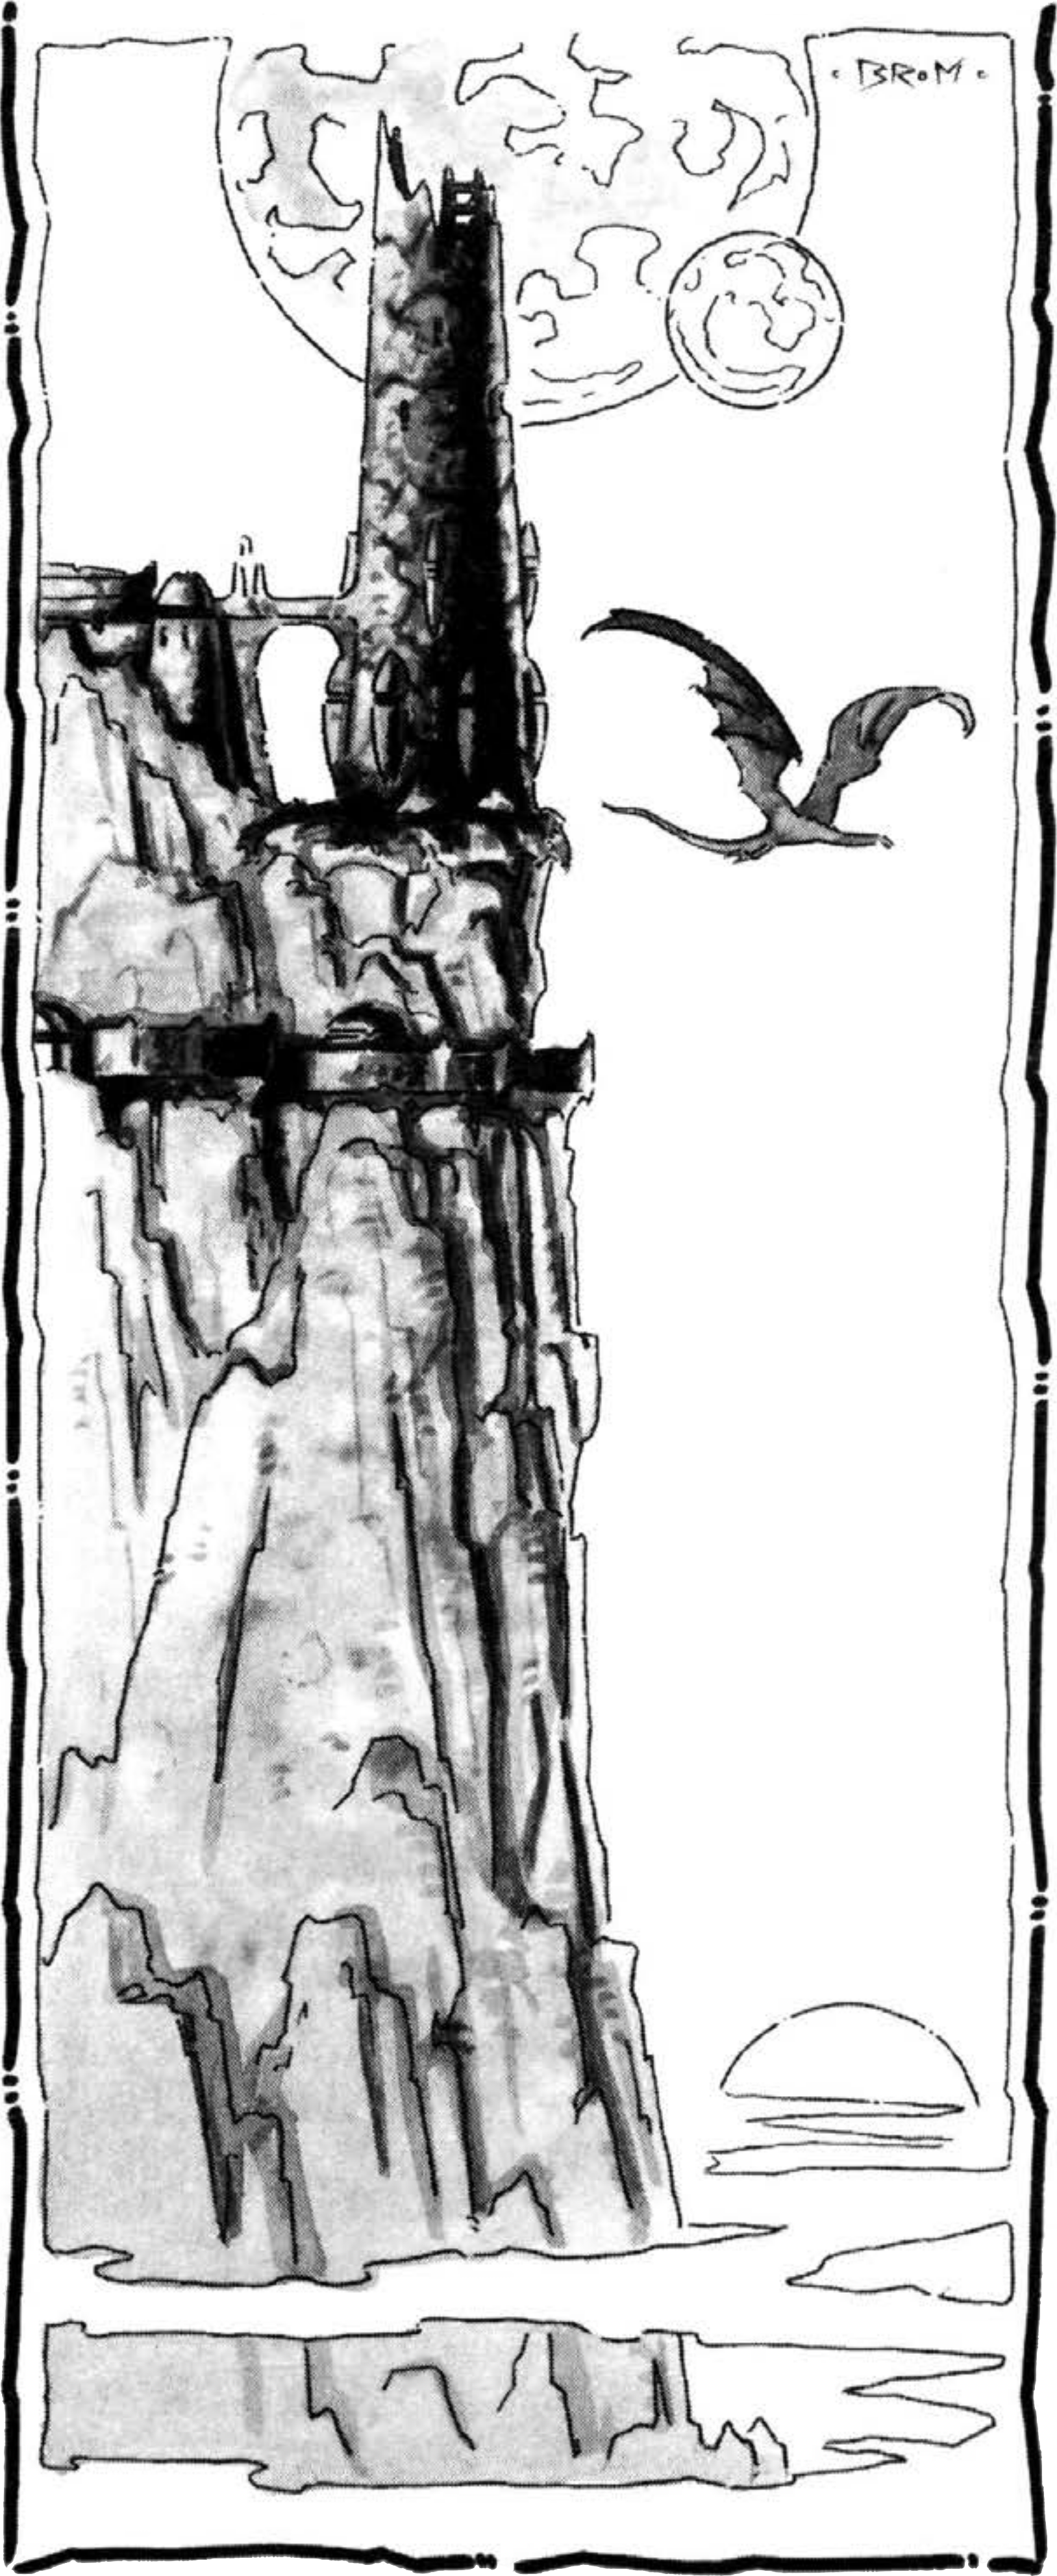
\includegraphics[width=\columnwidth]{images/tower-1.png}
\end{figure}

\Chapter{Abilities}
{Life is a mysterious and resilient thing. Even in the starkest wastes of Athas, the careful observer finds it clinging to the horns of sand dunes, peeking out from beneath wind-raked boulders, and creeping along the cracked plains of sun-baked clay.
To survive, almost every form of life has become a monster. On the increasingly infertile world of Athas, these adaptations have taken an almost diabolical turn. The land is so barren that every form of life, to one extent or another, is both predator and prey.}
{The Wanderer's Journal}
\Chapter{Abilities}
{Life is a mysterious and resilient thing. Even in the starkest wastes of Athas, the careful observer finds it clinging to the horns of sand dunes, peeking out from beneath wind-raked boulders, and creeping along the cracked plains of sun-baked clay.
To survive, almost every form of life has become a monster. On the increasingly infertile world of Athas, these adaptations have taken an almost diabolical turn. The land is so barren that every form of life, to one extent or another, is both predator and prey.}
{The Wanderer's Journal}

\Capitalize{E}{ach} character in {\tableheader Dark Sun} has six abilities: Strength (abbreviated Str), Dexterity (Dex), Constitution (Con), Intelligence (Int), Wisdom (Wis), and Charisma (Cha). Each of your abilities above average gives you a bonus on certain die rolls, and abilities below average give you a penalty on other die rolls.

\section{Ability Scores}

Previous editions used a rolling method that produced, on average, higher stats. This was supposed to convey that Athas was a much harsher world than normal D\&D campaign worlds, and that its denizens had adapted to compensate. However, the meaning of an attribute has changed in 3rd edition, and attributes start having a positive effect much sooner than they did in 2nd edition. Whereas many stats didn't start having a positive effect until they were at least 14, now as low as 12 have a positive effect. Using higher overall attributes for characters in {\tableheader Dark Sun} actually makes it easier for characters to survive and overcome obstacles that should be challenging, which would mean that the effective difficulty of a campaign would actually be lower using this stat generation method.

% \subsection{Creating Ability Scores}
% There are two methods for creating ability scores for your character: randomly or via point buy.  The average ability score for the typical commoner is 10 or 11, but your character is not typical. The most common ability scores for player characters (PCs) are 12 and 13.

% \subsubsection{Random Generation}
% To create an ability score for your character, roll 4d6. Disregard the lowest die roll and sum the rest. The result is a number between 3 (horrible) and 18 (tremendous)
% .
% Make this roll six times, recording each result on a piece of paper. Once you have six scores, assign each score to one of the six abilities.

% \subsubsection{Point Buy}
% All abilities scores start at 8. Take a number of points according to the type of your campaign to spread out among all abilities. For ability scores of 14 or lower, you buy additional points on a 1-for-1 basis. For ability scores higher than 14, it costs a little more.

% \Table{}{C C C C}{\tableheader Ability Score & \tableheader Point Cost & \tableheader Ability Score & \tableheader Point Cost \\
%   9 & 1 & 14 & 6 \\
%   10 & 2 & 15 & 8 \\
%   11 & 3 & 16 & 10 \\
%   12 & 4 & 17 & 13 \\
%   13 & 5 & 18 & 16}

% \Table{}{X r}{\tableheader Type of Campaign & \tableheader Points Allowed\\
%   Low-powered campaign & 15 points \\
%   Challenging campaign & 22 points \\
%   Normal campaign & 25 points \\
%   Tougher campaign & 28 points \\
%   High-powered campaign & 32 points}

\subsection{Ability Modifiers}

Each ability, after changes made because of race, has a modifier ranging from $-5$ to +5. \tabref{Ability Modifiers and Bonus Spells} shows the modifier for each score. It also shows bonus spells, which you'll need to know about if your character is a spellcaster.

The modifier is the number you apply to the die roll when your character tries to do something related to that ability. You also use the modifier with some numbers that aren't die rolls. A positive modifier is called a bonus, and a negative modifier is called a penalty.

\BigTable{Ability Modifiers and Bonus Spells}{X c C C C C C C C C C C}{
  \hline
  \rowcolor{white}
  & & \multicolumn{10}{c}{\tableheader Bonus Spells (by spell level)} \\
  \hline
  \rowcolor{white}
  \tableheader Score & \tableheader Modifier & \tableheader 0 & \tableheader 1st & \tableheader 2nd & \tableheader 3rd & \tableheader 4th & \tableheader 5th & \tableheader 6th & \tableheader 7th & \tableheader 8th & \tableheader 9th \\
  1 & $-5$ & \cellcolor{TableColor}&\cellcolor{TableColor}&\cellcolor{TableColor}&\cellcolor{TableColor}&\cellcolor{TableColor}&\cellcolor{TableColor}&\cellcolor{TableColor}&\cellcolor{TableColor}&\cellcolor{TableColor}&\cellcolor{TableColor}\\
  2-3 & $-4$ & \cellcolor{TableColor}&\cellcolor{TableColor}&\cellcolor{TableColor}&\cellcolor{TableColor}&\cellcolor{TableColor}&\cellcolor{TableColor}&\cellcolor{TableColor}&\cellcolor{TableColor}&\cellcolor{TableColor}&\cellcolor{TableColor}\\
  4-5 & $-3$ & \cellcolor{TableColor}&\cellcolor{TableColor}&\cellcolor{TableColor}&\cellcolor{TableColor}&\cellcolor{TableColor}&\cellcolor{TableColor}&\cellcolor{TableColor}&\cellcolor{TableColor}&\cellcolor{TableColor}&\cellcolor{TableColor}\\
  6-7 & $-2$ & \cellcolor{TableColor}&\cellcolor{TableColor}&\cellcolor{TableColor}&\cellcolor{TableColor}&\cellcolor{TableColor}&\cellcolor{TableColor}&\cellcolor{TableColor}&\cellcolor{TableColor}&\cellcolor{TableColor}&\cellcolor{TableColor}\\
  8-9 & $-1$ &\multicolumn{10}{c}{\multirow{-5}{*}{\bfseries Can't cast spells tied to this ability}}\\
  10-11 & 0 &&&&&&&&&&\\
  12-13 & +1 && 1 &&&&&&&&\\
  14-15 & +2 && 1 & 1 &&&&&&&\\
  16-17 & +3 && 1 & 1 & 1 &&&&&&\\
  18-19 & +4 && 1 & 1 & 1 & 1 &&&&&\\
  20-21 & +5 && 2 & 1 & 1 & 1 & 1 &&&&\\
  22-23 & +6 && 2 & 2 & 1 & 1 & 1 & 1 &&&\\
  24-25 & +7 && 2 & 2 & 2 & 1 & 1 & 1 & 1 &&\\
  26-27 & +8 && 2 & 2 & 2 & 2 & 1 & 1 & 1 & 1 &\\
  28-29 & +9 && 3 & 2 & 2 & 2 & 2 & 1 & 1 & 1 & 1 \\
  30-31 & +10 && 3 & 3 & 2 & 2 & 2 & 2 & 1 & 1 & 1 \\
  32-33 & +11 && 3 & 3 & 3 & 2 & 2 & 2 & 2 & 1 & 1 \\
  34-35 & +12 && 3 & 3 & 3 & 3 & 2 & 2 & 2 & 2 & 1 \\
  36-37 & +13 && 4 & 3 & 3 & 3 & 3 & 2 & 2 & 2 & 2 \\
  38-39 & +14 && 4 & 4 & 3 & 3 & 3 & 3 & 2 & 2 & 2 \\
  40-41 & +15 && 4 & 4 & 4 & 3 & 3 & 3 & 3 & 2 & 2
}

\BigTable{Ability Scores and Bonus Power Points}{l C C C C C C C C C C C C C C C C C C C C}{
  \hline
  \rowcolor{white}
  & \multicolumn{20}{c}{\tableheader Bonus Power Points (by class level)} \\
  \hline
  \rowcolor{white}
\tableheader Score & \tableheader 1st & \tableheader 2nd & \tableheader 3rd & \tableheader 4th & \tableheader 5th & \tableheader 6th & \tableheader 7th & \tableheader 8th & \tableheader 9th & \tableheader 10th & \tableheader 11th & \tableheader 12th & \tableheader 13th & \tableheader 14th & \tableheader 15th & \tableheader 16th & \tableheader 17th & \tableheader 18th & \tableheader 19th & \tableheader 20th \\
10-11 &&&&&&&&&&&&&&&&&&&&\\
12-13 && 1 & 1 & 2 & 2 & 3 & 3 & 4 & 4 & 5 & 5 & 6 & 6 & 7 & 7 & 8 & 8 & 9 & 9 & 10 \\
14-15 & 1 & 2 & 3 & 4 & 5 & 6 & 7 & 8 & 9 & 10 & 11 & 12 & 13 & 14 & 15 & 16 & 17 & 18 & 19 & 20 \\
16-17 & 1 & 3 & 4 & 6 & 7 & 9 & 10 & 12 & 13 & 15 & 16 & 18 & 19 & 21 & 22 & 24 & 25 & 27 & 28 & 30 \\
18-19 & 2 & 4 & 6 & 8 & 10 & 12 & 14 & 16 & 18 & 20 & 22 & 24 & 26 & 28 & 30 & 32 & 34 & 36 & 38 & 40 \\
20-21 & 2 & 5 & 7 & 10 & 12 & 15 & 17 & 20 & 22 & 25 & 27 & 30 & 32 & 35 & 37 & 40 & 42 & 45 & 47 & 50 \\
22-23 & 3 & 6 & 9 & 12 & 15 & 18 & 21 & 24 & 27 & 30 & 33 & 36 & 39 & 42 & 45 & 48 & 51 & 54 & 57 & 60 \\
24-25 & 3 & 7 & 10 & 14 & 17 & 21 & 24 & 28 & 31 & 35 & 38 & 42 & 45 & 49 & 52 & 56 & 59 & 63 & 66 & 70 \\
26-27 & 4 & 8 & 12 & 16 & 20 & 24 & 28 & 32 & 36 & 40 & 44 & 48 & 52 & 56 & 60 & 64 & 68 & 72 & 76 & 80 \\
28-29 & 4 & 9 & 13 & 18 & 22 & 27 & 31 & 36 & 40 & 45 & 49 & 54 & 58 & 63 & 67 & 72 & 76 & 81 & 85 & 90 \\
30-31 & 5 & 10 & 15 & 20 & 25 & 30 & 35 & 40 & 45 & 50 & 55 & 60 & 65 & 70 & 75 & 80 & 85 & 90 & 95 & 100 \\
32-33 & 5 & 11 & 16 & 22 & 27 & 33 & 38 & 44 & 49 & 55 & 60 & 66 & 71 & 77 & 82 & 88 & 93 & 99 & 104 & 110 \\
34-35 & 6 & 12 & 18 & 24 & 30 & 36 & 42 & 48 & 54 & 60 & 66 & 72 & 78 & 84 & 90 & 96 & 102 & 108 & 114 & 120 \\
36-37 & 6 & 13 & 19 & 26 & 32 & 39 & 45 & 52 & 58 & 65 & 71 & 78 & 84 & 91 & 97 & 104 & 110 & 117 & 123 & 130 \\
38-39 & 7 & 14 & 21 & 28 & 35 & 42 & 49 & 56 & 63 & 70 & 77 & 84 & 91 & 98 & 105 & 112 & 119 & 126 & 133 & 140 \\
40-41 & 7 & 15 & 22 & 30 & 37 & 45 & 52 & 60 & 67 & 75 & 82 & 90 & 97 & 105 & 112 & 120 & 127 & 135 & 142 & 150}

\subsection{Abilities, Spellcasters and \hskip4em Manifesters}
The ability that governs bonus spells depends on what type of spellcaster your character is: Intelligence for wizards; Wisdom for clerics, druids, and rangers; or Charisma for templars. In addition to having a high ability score, a spellcaster must be of high enough class level to be able to cast spells of a given spell level.

Psionic classes also depend on abilities for additional power: Intelligence for psions, Wisdom for psychic warriors, and Charisma for wilders. The modifier for this ability is referred to as your key ability modifier. If your character's key ability score is 9 or lower, you can't manifest powers from that psionic class.

Just as a high Intelligence score grants bonus spells to a wizard and a high Wisdom score grants bonus spells to a cleric, a character who manifests powers (psions, psychic warriors, and wilders) gains bonus power points according to his key ability score. Refer to \tabref{Ability Scores and Bonus Power Points}.

\subsubsection{How To Determine Bonus Power Points}
Your key ability score grants you additional power points equal to your key ability modifier $\times$ your manifester level $\times$ \onehalf. \tabref{Ability Scores and Bonus Power Points} shows these calculations for class levels 1st through 20th and key ability scores from 10 to 41.

\section{The Abilities}
Each ability partially describes your character and affects some of his or her actions.

\subsection{Strength (Str)}
Strength measures your character's muscle and physical power. This ability is especially important for gladiators, fighters, barbarians, and rangers because it helps them prevail in combat. Strength also limits the amount of equipment your character can carry.

You apply your character's Strength modifier to:
\begin{itemize*}
\item Melee attack rolls.
\item Damage rolls when using a melee weapon or a thrown weapon (including a sling). (Exceptions: Off-hand attacks receive only one-half the character's Strength bonus, while two-handed attacks receive one and a half times the Strength bonus. A Strength penalty, but not a bonus, applies to attacks made with a bow that is not a composite bow.)
\item \skill{Climb}, \skill{Jump}, and \skill{Swim} checks. These are the skills that have Strength as their key ability.
\item Strength checks (for breaking down doors and the like).
\end{itemize*}

\subsection{Dexterity (Dex)}
Dexterity measures hand-eye coordination, agility, reflexes, and balance. This ability is the most important one for rogues, and bards, but it's also high on the list for characters who typically wear light or medium armor (gladiators, rangers, wilders, and barbarians) or no armor at all (psions and wizards), and for anyone who wants to be a skilled archer.

You apply your character's Dexterity modifier to:
\begin{itemize*}
\item Ranged attack rolls, including those for attacks made with bows, crossbows, throwing axes, and other ranged weapons.
\item Armor Class (AC), provided that the character can react to the attack.
\item Reflex saving throws, for avoiding fireballs and other attacks that you can escape by moving quickly.
\item \skill{Balance}, \skill{Escape Artist}, \skill{Hide}, \skill{Move Silently}, \skill{Open Lock}, \skill{Ride}, \skill{Sleight of Hand}, \skill{Tumble}, and \skill{Use Rope} checks. These are the skills that have Dexterity as their key ability.
\end{itemize*}
\subsection{Constitution (Con)}
Constitution represents your character's health and stamina. A Constitution bonus increases a character's hit points, so the ability is important for all classes.

You apply your character's Constitution modifier to:
\begin{itemize*}
\item Each roll of a Hit Die (though a penalty can never drop a result below 1---that is, a character always gains at least 1 hit point each time he or she advances in level).
\item Fortitude saving throws, for resisting poison and similar threats.
\item \skill{Concentration} checks. Concentration is a skill, important to spellcasters, that has Constitution as its key ability.
\end{itemize*}

If a character's Constitution score changes enough to alter his or her Constitution modifier, the character's hit points also increase or decrease accordingly.

\subsection{Intelligence (Int)}
Intelligence determines how well your character learns and reasons. This ability is important for wizards because it affects how many spells they can cast, how hard their spells are to resist, and how powerful their spells can be. It's also important for any character who wants to have a wide assortment of skills.

You apply your character's Intelligence modifier to:
\begin{itemize*}
\item The number of languages your character knows at the start of the game.
\item The number of skill points gained each level. (But your character always gets at least 1 skill point per level.)
\item \skill{Appraise}, \skill{Craft}, \skill{Decipher Script}, \skill{Disable Device}, \skill{Forgery}, \skill{Knowledge}, \skill{Search}, and \skill{Spellcraft} checks. These are the skills that have Intelligence as their key ability.
\end{itemize*}

A wizard gains bonus spells based on her Intelligence score. The minimum Intelligence score needed to cast a wizard spell is 10 + the spell's level.

An animal has an Intelligence score of 1 or 2. A creature of human-like intelligence has a score of at least 3.

\subsection{Wisdom (Wis)}
Wisdom describes a character's willpower, common sense, perception, and intuition. While Intelligence represents one's ability to analyze information, Wisdom represents being in tune with and aware of one's surroundings. Wisdom is the most important ability for clerics and druids, and it is also important for rangers. If you want your character to have acute senses, put a high score in Wisdom. Every creature has a Wisdom score.

You apply your character's Wisdom modifier to:
\begin{itemize*}
\item Will saving throws (for negating the effect of charm person and other spells).
\item \skill{Heal}, \skill{Listen}, \skill{Profession}, \skill{Sense Motive}, \skill{Spot}, and \skill{Survival} checks. These are the skills that have Wisdom as their key ability.
\item Clerics, druids, and rangers get bonus spells based on their Wisdom scores. The minimum Wisdom score needed to cast a cleric, druid, or ranger spell is 10 + the spell's level.
\end{itemize*}

\subsection{Charisma (Cha)}
Charisma measures a character's force of personality, persuasiveness, personal magnetism, ability to lead, and physical attractiveness. This ability represents actual strength of personality, not merely how one is perceived by others in a social setting. Charisma is most important for templars. It is also important for clerics, since it affects their ability to turn undead. Every creature has a Charisma score.

You apply your character's Charisma modifier to:
\begin{itemize*}
\item \skill{Bluff}, \skill{Diplomacy}, \skill{Disguise}, \skill{Gather Information}, \skill{Handle Animal}, \skill{Intimidate}, \skill{Perform}, and \skill{Use Magic Device} checks. These are the skills that have Charisma as their key ability.
\item Checks that represent attempts to influence others.
\item Turning checks for clerics and templars attempting to turn zombies, vampires, and other undead.
\end{itemize*}

Sorcerers and bards get bonus spells based on their Charisma scores. The minimum Charisma score needed to cast a sorcerer or bard spell is 10 + the spell's level.

\subsection{Changing Ability Scores}
When an ability score changes, all attributes associated with that score change accordingly. A character does not retroactively get additional skill points for previous levels if she increases her intelligence.


\Chapter{Character Races}
{I live in a world of fire and sand. The crimson sun scorches the life from anything that crawls or flies, and storms of sand scour the foliage from the barren ground. Lightning strikes from the cloudless sky, and peals of thunder roll unexplained across the vast tablelands. Even the wind, dry and searing as a kiln, can kill a man with thirst.}
{The Wanderer's Journal}
\Chapter{Character Races}
{I live in a world of fire and sand. The crimson sun scorches the life from anything that crawls or flies, and storms of sand scour the foliage from the barren ground. Lightning strikes from the cloudless sky, and peals of thunder roll unexplained across the vast tablelands. Even the wind, dry and searing as a kiln, can kill a man with thirst.}
{The Wanderer's Journal}

\Capitalize{A}{thas} is a world of many races, from the gith who wander the deserts, to the tareks, too stubborn to know when they have died. Giants terrorize the Silt Sea, while belgoi steal grown men in the night. The magic of the Pristine Tower produces the New Races; most never see a second generation. Despite the variety of intelligent life, only a few races have the numbers to significantly impact the politics of the Tablelands.

Though the races of the {\tableheader Dark Sun} campaign setting resemble those of other campaign worlds, it is frequently in name only. The insular elves roam the Tablelands, trusted by no one but their own tribe-mates. Halflings are feral creatures, possessed of a taste for human flesh. Hairless dwarves work endlessly, their entire perception of the world filtered through the lens of a single, all-consuming task. Unsleeping thri-kreen roam the wastes, always hunting their next meal.

\section{Racial Characteristics}

\subsection{Ability Adjustments}

Find your character's race on \tabref{Athasian Racial Ability Adjustments} and apply the adjustments to your character's ability scores. If these changes put your score above 18 or below 3, that's okay, except in the case of Intelligence, which does not go below 3 for characters.

\subsection{Level Adjustment}

To determine the effective character level (ECL) of a character, add its race's level adjustment (LA) to its character class levels.

Use ECL instead of character level to determine how many experience points a character needs to reach its next level. Also use ECL to determine starting wealth for a character.

\subsection{Favored Class}

Each race's favored class is also given on \tabref{Athasian Racial Ability Adjustments}. A character's favored class doesn't count against him or her when determining experience point penalties for multiclassing.

\BigTablePair{Athasian Racial Ability Adjustments}{l l C p{6cm} p{2cm} l}{
\tableheader Race & \tableheader Type (Subtype) & \tableheader LA & \tableheader Ability Adjustments & \tableheader Favored Class & \tableheader Languages \\
Human & Humanoid (human) &&& Any & Common \\
Aarakocra & Monstrous Humanoid & +1 & $-2$ Strength, +4 Dexterity, $-2$ Charisma & Cleric & Auran, Common \\
Dwarf & Humanoid (dwarf) && +2 Constitution, $-2$ Charisma & Fighter & Common, Dwarven \\
Elf & Humanoid (elf) && +2 Dexterity, $-2$ Constitution & Rogue & Common, Elven \\
Half-elf & Humanoid (elf) && +2 Dexterity, $-2$ Charisma & Any & Common, Elven \\
Half-giant & Giant & +2 & +8 Strength, $-2$ Dexterity, +4 Constitution, \newline $-4$ Intelligence, $-4$ Wisdom, $-4$ Charisma & Barbarian & Common \\
Halfling & Humanoid (halfling) && $-2$ Strength, +2 Dexterity & Ranger & Halfling \\
Mul & Humanoid (dwarf) & +1 & +4 Strength, +2 Constitution, $-2$ Charisma & Gladiator & Common \\
Pterran & Humanoid (pterran) && $-2$ Dexterity, +2 Wisdom, +2 Charisma & Druid, ranger,\newline or telepath & Saurian \\
Thri-kreen & Monstrous Humanoid & +2 & +2 Strength, +4 Dexterity, $-2$ Intelligence, \newline +2 Wisdom, $-4$ Charisma & Psychic warrior & Kreen}

\subsection{Race And Languages}

Only races that live in the reach of the city-states know how to speak Common. A aarakocra, dwarf, elf, half-elf, halfling, pterran, or thri-kreen also speaks a racial language, as appropriate. A character who has an Intelligence bonus at 1st level speaks other languages as well, one extra language per point of Intelligence bonus as a starting character.

\textbf{Literacy}: The ability to read has been outlawed for thousands of years by the sorcerer-kings. All characters in a {\tableheader Dark Sun} campaign start without the ability to read or write.

\textbf{Class-Related Languages}: Clerics, druids, templars, and wizards can choose certain languages as bonus languages even if they're not on the lists found in the race descriptions. These class-related languages are as follows:

\textit{Cleric}: Aquan, Auran, Ignan, Terran.

\textit{Druid}: Sylvan.

\textit{Templar}: Templar's City-State language.

\textit{Wizard}: Draconic.

\section{Humans}
\Quote{Humans are fools, and hopelessly naive as well. They outnumber us; they are everywhere, and yet they have no more sense of their strength than a rat. Let us hope that the Datto remain that way.}{Dukkoti Nightrunner, elven warrior}

While not the strongest race, nor the quickest, humans have dominated the Tablelands for the last three thousand years.

\textbf{Personality:} More than other races, human personality is shaped by their social standing and background.

\textbf{Physical Description:} Human males average 1.8 meter tall and 100 kg, while smaller females average 1.65 meters and 70 kg. Color of eyes, skin, and hair, and other physical features vary wildly; enlarged noses, webbed feet or extra digits are not uncommon.

\textbf{Relations:} Human treatment of other races is usually based on what their culture has taught them. In large settlements, such as in city-states, close proximity with many races leads to a suspicious unfriendly tolerance.

\textbf{Alignment:} Humans have no racial tendency toward any specific alignment.

\textbf{Human Lands:} Humans can be found anywhere, from the great city-states to the barren wastes.

\textbf{Magic:} Most humans fear and hate arcane magic, forming mobs to kill vulnerable wizards.

\textbf{Psionics:} Humans see the Way as a natural part of daily life, and readily become psions.

\textbf{Religion:} Most humans pay homage to the elements. Draji and Gulgs often worship their monarchs.

\textbf{Language:} Most humans speak the common tongue. Nobles and artisans within a given city-state usually speak the city language, but slaves typically only speak Common.

\textbf{Names:} Nobles, artisans and traders use titles or surnames; others some simply use one name.

\textbf{Male Names:} Agis of Asticles, King Tithian, Lord Vordon, Pavek, Trenbull Al'Raam'ke

\textbf{Female Names:} Akassia, General Zanthiros, Lady Essen of Rees, Neeva, Sadira

\textbf{Adventurers:} Some human adventurers seek treasure; others adventure for religious purposes as clerics or druids; others seek companionship or simply survival.

\subsection{Human Racial Traits}
\begin{itemize*}
  \item Medium: As Medium creatures, humans have no special bonuses or penalties due to their size. 
  \item Human base land speed is 9 meters.
  \item 1 extra feat at 1st level.
  \item 4 extra skill points at 1st level and 1 extra skill point at each additional level.
  \item Automatic Language: Common. Bonus Languages: Any (other than secret languages, such as Druidic). See the \skill{Speak Language} skill.
  \item Favored Class: Any. When determining whether a multiclass human takes an experience point penalty, his or her highest-level class does not count.
\end{itemize*}

\section{Aarakocra}
\Quote{You are all slaves. You all suffer from the tyranny of the ground. Only in the company of clouds will you find the true meaning of freedom.}{Kekko Cloud-Brother, aarakocra cleric}

Aarakocra are the most commonly encountered bird-people of the Tablelands. Some are from Winter Nest in the White Mountains near Kurn, while others are from smaller tribes scattered in the Ringing Mountains and elsewhere. These freedom-loving creatures rarely leave their homes high in the mountains, but sometimes, either as young wanderers or cautious adventurers, they venture into the inhabited regions of the Tablelands.

\textbf{Personality:} These bird-people can spend hours riding the wind currents of the mountains, soaring in the olive-tinged Athasian sky. While traveling, aarakocra prefer to fly high above to get a good view all around their location and detect any threats well in advance. When they stop to rest, they tend to perch on high peaks or tall buildings. Enclosed spaces threaten the aarakocra, who have a racial fear of being anywhere they cannot stretch their wings. This claustrophobia affects their behavior. Unless it is absolutely necessary, no aarakocra will enter a cave or enclosed building, or even a narrow canyon.

\textbf{Physical Description:} Aarakocra stand 2 to 2.4 meters tall, with a wingspan of about 6 meters. They have black eyes, gray beaks, and from a distance they resemble lanky disheveled vultures. Aarakocran plumage ranges from silver white to brown, even pale blue. Male aarakocra weigh around 50 kg, while females average 42.5 kg. An aarakocra's beak comprises much of its head, and it can be used in combat. At the center of their wings, aarakocra have three-fingered hands with an opposable thumb, and the talons of their feet are just as dexterous. While flying, aarakocra can use their feet as hands, but while walking, they use their wing-hands to carry weapons or equipment. Aarakocra have a bony plate in their chest (the breastbone), which provides protection from blows. However, most of their bones are hollow and brittle and break more easily than most humanoids. The aarakocra's unusual build means they have difficulty finding armor, unless it has been specifically made for aarakocra. Aarakocra usually live between 30 and 40 years.

\textbf{Relations:} Aarakocra zealously defend their homeland. They are distrustful of strangers that venture onto their lands. Many of the southern tribes exact tolls on all caravans passing through their lands, sometimes kidnapping scouts or lone riders until tribute is paid. Tribute can take the form of livestock or shiny objects, which aarakocra covet. Some evil tribes may attack caravans without provocation. Aarakocra have great confidence and pride in their ability to fly, but have little empathy for land-bound races.

\textbf{Alignment:} Aarakocra tend towards neutrality with regard to law or chaos. With respect to good and evil, Aarakocran tribes usually follow the alignment of their leader. A tribe whose leader is neutral good will contain lawful good, neutral good, chaotic good and neutral members, with most members being neutral good. Aarakocra, even good ones, rarely help out strangers.

\textbf{Aarakocran Lands:} Most Aarakocran communities are small nomadic tribes. Some prey on caravans, while others or build isolated aeries high in the mountains. The least xenophobic aarakocra generally come from Winter Nest, in the White Mountains, a tribe allied with the city-state of Kurn. Of all the human communities, only Kurn builds perches especially made for aarakocra to rest and do business. In contrast, king Daskinor of Eldaarich has ordered the capture and extermination of all aarakocra. Other human communities tolerate Aarakocran characters but do not welcome them. Merchants will do business with aarakocra as long as they remain on foot. Most land-bound creatures are suspicious of strange creatures that fly over their herds or lands unannounced, and templars, even in Kurn, have standing orders to attack creatures that fly over the city walls without permission.

\textbf{Magic:} Most Aarakocran tribes shun wizardly magic, but a few evil tribes have defilers, and one prominent good-aligned tribe, Winter's Nest, has several preservers.

\textbf{Psionics:} Aarakocra are as familiar with psionics as other races of the tablelands. They particularly excel in the psychoportation discipline. In spite of their low strength and constitutions, they excel as psychic warriors, often using ranged touch powers from above to terrifying effect.

\textbf{Religion:} Aarakocran shamans are usually air clerics, sometimes sun clerics, and occasionally druids. Most rituals of Aarakocran society involve the summoning of an air elemental, or Hraak'thunn in Auran (although an aarakocra would call their language Silvaarak, and not Auran). Summoned air elementals are often used in an important ritual, the Hunt. The Aarakocran coming of age ceremony involves hunting the great beasts found in the Silt Sea.

\textbf{Language:} Athasian aarakocra speak Auran. Aarakocra have no written language of their own, though some of the more sophisticated tribes have borrowed alphabets from their land-bound neighbors. Regardless of the language spoken, aarakocra do not possess lips, and therefore cannot even approximate the 'm', 'b' or 'p' sounds. They have difficulty also with their 'f's and 'v's, and tend to pronounce these as 'th' sounds.

\textbf{Male Names:} Akthag, Awnunaak, Cawthra, Driikaak, Gazziija, Kraah, Krekkekelar, Nakaaka, Thraka.

\textbf{Female Names:} Arraako, Kariko, Kekko, Lisako, Troho.

\textbf{Tribal Names:} Cloud Gliders, Sky Divers, Peak Masters, Far Eyes, Brothers of the Sun.

\textbf{Adventurers:} Adventuring aarakocra are usually young adults with a taste for the unknown. They are usually curious, strong-minded individuals that wish to experience the lives of the land-bound peoples. Good tribes see these young ones as undisciplined individuals, but can tolerate this behavior. Evil tribes may view this sort of adventurous behavior as treacherous, and may even hunt down the rogue member.

\subsection{Aarakocra Society}
The aarakocra have a tribal society. The civilized tribes of Winter Nest form the largest known community of aarakocra in the Tyr region. Though their communities are lead by a chieftain, the aarakocra have a great love of personal freedom. So while the chieftain makes all major decisions for the community, unless she consults with the tribal elders and builds a strong consensus within the tribe first, her decisions may be ignored.

Air and sun shamans play an important role in aarakocra societies. Aarakocra worship the sun because it provides them with the thermals they need to soar. The air shamans of Winter Nest lead their community in daily worship of the air spirits.

Aarakocra of Winter Nest have a deep and abiding respect for the gifts of nature and little patience for those who abuse those gifts. They look after the natural resources of the White Mountains and have been known to punish those who despoil or abuse them.

In more primitive societies, female aarakocra rarely travel far from the safety of the nest, and focus solely on raising the young. In Winter Nest, both sexes participate in all aspects of society, with females more often elected by the elders to be chieftains.

Aarakocra believe that their ability to fly makes them superior to all other races and thus they have great confidence and pride in themselves. Though they often express sympathy for people unable to fly, this more often comes across as condescending.

Aarakocra are carnivores, but do not eat intelligent prey.
\subsection{Roleplaying Suggestions}
Loneliness doesn't bother you like it bothers people of other races. You loathe the heat and stink of the cities, and long for cold, clean mountain air. The spectacle and movement of so many sentient beings fascinates you, but watching them from above satisfies your curiosity. The very thought of being caught in a crowd of creatures, pinned so tight that you can't move your own wings, fills you with terror.

You are friendly enough with people of other races, provided they respect your physical distance, and are willing to be the ones that approach you. You form relationships with individuals, but don't involve yourself in the politics of other racial communities - in such matters you prefer to watch from above and to keep your opinions to yourself unless asked.

You prefer to enter buildings through a window rather than through a door. Your instincts are to keep several scattered, hidden, nests throughout the areas that you travel regularly: one never knows when one might need a high place to rest. Remember your love of heights and claustrophobia, and rely on Aarakocran skills and tactics (dive-bombing). Take advantage of your flying ability to scout out the area and keep a ``bird's eye view'' of every situation.

\subsection{Aarakocra Racial Traits}
\begin{itemize*}
    \item $-2$ Strength, +4 Dexterity, $-2$ Constitution: Aarakocra have keen reflexes, but their lightweight bones are fragile.
    \item Monstrous Humanoid: Aarakocra are not subject to spells or effects that affect humanoids only, such as charm person or dominate person.
    \item Medium: As Medium creatures, aarakocra have no special bonuses or penalties due to size.
    \item Low-light vision: Aarakocra can see twice as far as a human in moonlight and similar conditions of poor illumination, retaining the ability to distinguish color and detail.
    \item Aarakocra base land speed is 6 meters, and can fly with a movement rate of 27 meters (average maneuverability).
    \item +6 racial bonus to \skill{Spot} checks in daylight. Aarakocra have excellent vision.
    \item Natural Armor: Aarakocra have +1 natural armor bonus due to their bone chest plate that provides some protection from blows.
    \item Natural Weaponry: An aarakocra can rake with its claws for 1d3 points of damage, and use its secondary bite attack for 1d2 points of damage.
    \item Claustrophobic: Aarakocra receive a $-2$ morale penalty on all rolls when in an enclosed space. Being underground or in enclosed buildings is extremely distressing for them.
    \item Aerial Dive: Aarakocra can make dive attacks. A dive attack works just like a charge, but the diving creature must move a minimum of 9 meters. If attacking with a lance, the aarakocra deals double damage on a successful attack. Optionally, the aarakocra can make a full attack with its natural weapons (two claws and one bite) at the end of the charge, dealing normal damage.
    \item Automatic Languages: Auran and Common. Bonus Languages: Elven, Gith, and Saurian. Aarakocra often learn the languages of their allies and enemies.
    \item Favored Class: Cleric. A multiclass aarakocra's cleric class does not count when determining whether he takes an experience point for multiclassing.
    \item Level Adjustment: +1. Aarakocra are slightly more powerful and gain levels more slowly than most of the humanoid races of the Tablelands.
\end{itemize*}
\section{Dwarves}
\Quote{The worst thing you can say to a dwarf is 'It can't be done.' If he's already decided to do it, he may never speak to you again. If he hasn't decided to take up the task, he may commit imself to it simply out of spite. 'Impossible' is not a concept most dwarves understand. Anything can be done, with enough determination.}{Sha'len, Nibenese trader}

Dwarves form a good part of the people encountered in the Tablelands. These strong and devoted beings live to fulfill their focus, a task they choose to devote their lives to. Stubborn and strong-minded, dwarves make good companions, even though their usual focused nature can tend to be bothersome.

\textbf{Personality:} Dwarves prefer to occupy themselves with meaningful tasks, and often approach these tasks with an intensity rarely seen in other races. As such, dwarves make excellent laborers, and take great pride in their accomplishments. However, their stubbornness can lead to difficulties. Dwarves will sometimes fail to listen to reason, attempting to accomplish what are impossible tasks. Dwarves live for their focus. Dwarves that die while being unable to complete their focus return from the dead as banshees to haunt their unfinished work. A dwarf also rarely divulges his focus to anyone.

\textbf{Physical Description:} The dwarves of the Tablelands stand 1.35 m to 1.5 m tall, with big muscular limbs and a strong build. They weigh on average 100 kg. Dwarves are hairless, and find the very idea of hair repulsive. They have deeply tanned skin, and rarely decorate it with tattoos. Dwarves can live up to 250 years.

\textbf{Relations:} A dwarf's relation with others is often a function of his focus. People that help the dwarf accomplish his focus or share his goals are treated with respect and considered good companions. There is little room for compromise, though, with those that disagree with the dwarf's focus. If they hinder the dwarf, they are considered obstacles that must be removed. Community is important to the dwarves. Dwarves have a very strong racial affinity. They rarely share their history with non-dwarves; it can take years for a stranger to gain enough trust to be admitted into a Dwarven family circle.

\textbf{Alignment:} Dwarves tend towards a lawful alignment, with most members either good or neutral. Their devotion to following the established hierarchy in their village means they tend to follow the rules, sometimes to the point of ridicule.

\textbf{Dwarven Lands:} There are three main Dwarven settlements in the Tablelands: Kled, located near the city-state of Tyr, and the twin villages of North and South Ledopolus located in the southwestern edge of the Tablelands. Some Dwarven communities have developed in the city-states and in some small villages, while other dwarves have taken up residence with the slave tribes of the wastes.

\textbf{Magic:} Like most peoples, dwarves have an aversion to wizardly magic, and they are the least amenable to changing their minds about anything. Dwarves rarely take to the wizardly arts; the few that do are usually shunned from respectable Dwarven society. Some dwarves will travel with a wizard who proves himself a worthy companion, but few dwarves will truly ever trust a wizard.

\textbf{Psionics:} Like almost everything that they do, dwarves take to psionics with a vengeance. They make formidable egoists and nomads.

\textbf{Religion:} Dwarven communities are ruled by their elders; dwarves are particularly devoted to their community leader, the Urhnomous. Dwarves typically worship elemental earth. Fire is sometimes worshiped for its destructive power and water for its healing nature. Air's intangibility and chaotic nature attracts few Dwarven worshipers. Dwarven druids are unusual, and tend to devote themselves to a particular area of guarded land.

\textbf{Language:} Dwarves have a long and proud oral history. They have an old written language, but this is mostly used for writing histories. Dwarves will not teach their ancient language to outsiders, they prefer to keep that knowledge to themselves. The Dwarven language is deep and throaty, composed of many guttural sounds and harsh exclamations. Most non-dwarves get raw throats if they try to speak Dwarven for more than a few hours.

\textbf{Names:} A dwarf's name is usually granted to him by his clan leader after he completes his first focus.

\textbf{Male Names:} Baranus, Biirgaz, Bontar, Brul, Caelum, Caro, Daled, Drog, Fyra, Ghedran, Gralth, Gram, Jurgan, Lyanius, Murd, Nati, Portek.

\textbf{Female Names:} Ardin, Erda, Ghava, Greshin, Gudak, Lazra, N'kadir, Palashi, Vashara.

\textbf{Adventurers:} Dwarves adventure for different reasons. Sometimes they may adventure in order to learn about the Tablelands, although these curious adventurers tend to be young and brash. Many adventuring dwarves travel the Tablelands to complete their focus because sometimes a task may take them away from their communities. Some search for ancient Dwarven villages and the treasures they contain.

\subsection{Dwarf Society}
No dwarf is more content than while working toward the resolution of some cause. This task, called a focus, is approached with single-minded direction for the dwarf's entire life, if need be, though most focuses require considerable less time.

Free dwarves form communities based on clans, and are much focused on family. Ties of blood are honored and respected above all others, except the focus. Family honor is important to every dwarf, because an act that brings praise or shame in one generation is passed down to the family members of the next generation. There is no concept in the minds of dwarves of not following these family ties.

Dwarven communities are found in many types of terrain, from mountains and deserts to near human cities. Most communities are small, rarely exceeding 300 members and are usually formed of extended families linked by a common ancestor. Community leaders are called Urhnomous (over-leader). Each clan is lead by an uhrnius (leader).

Most free dwarves earn their money through trade. Those that stand out in this category are Dwarven metal smiths and mercenaries. Most Athasians acknowledge Dwarven forged metal to be among the best. Some dwarves even act as metal scavengers, seeking steel scraps where ever they can be found to sell to the smiths. Dwarven mercenaries are highly prized because once their loyalty is purchased it is never changed.

\subsection{Roleplaying Suggestions}
Remember the intensity of your focus. Breaking or ignoring a focus has social, philosophical and spiritual repercussions. For someone to stand in the way of your focus is an assault on you. There is no greater satisfaction than fulfilling a difficult focus. Keep a serious, sober attitude nearly always. The only time you show your festive side is when you have recently fulfilled a focus, during the hours or days until you set a new focus.

Only during these brief days of fulfillment, and only to other dwarves and your most trusted non-Dwarven friends, do you show your full joy and sense of humor. But these days are also a time of vulnerability, for until you set a new focus you lose all of your special focus-related bonuses.

\subsection{Dwarven Focus}

A dwarf's focus is the central point of his existence. Nothing is more rewarding to a dwarf than to complete his focus. A focus must take at least a week to complete; anything less than that is too simple a task to be considered a focus. Dwarves receive a morale bonus working to complete a focus. The task must be directly related to the completion of the focus, however.

For example, Grelak, protector of his Dwarven community, makes the retrieval of a sacred book stolen during a raid his focus. After a week of gathering clues, he sets out to retrieve the artifact from its current possessor, who hides in a trading post two weeks away. On the way to the outpost, he encounters a wild lirr; while battling this foe, he receives his morale bonus, because he is trying to reach the book. Later, Grelak stops in Nibenay for some rest, and gets in a brawl. He doesn't receive any bonuses, because he isn't actively pursuing his focus.

\subsection{Dwarf Racial Traits}
\begin{itemize*}
    \item +2 Constitution, $-2$ Charisma: Dwarves are strong and sturdy, but their single-mindedness hinders them when dealing with others.
    \item Humanoid (dwarf): Dwarves are humanoid creatures with the dwarf subtype.
    \item Medium: As Medium creatures, dwarves have no special bonuses or penalties due to size.
    \item Darkvision: Dwarves can see in the dark up to 18 meters. Darkvision is black and white only, but it is otherwise like normal sight, and dwarves can function just fine with no light at all.
    \item Dwarven base land speed is 6 meters. However, dwarves can move at this speed even when wearing medium or heavy armor or when carrying a medium or heavy load (unlike other creatures whose speed is reduced in such situations).
    \item Stability: A dwarf gains a +4 bonus on ability checks made to resist being bull rushed or tripped when standing on the ground (but not when climbing, flying, riding, or otherwise not standing firmly on the ground).
    \item +2 racial bonus on saving throws against poison.
    \item Weapon Familiarity: To dwarves, the urgrosh is treated as a martial rather than exotic weapon.
    \item +2 racial bonus on saving throws against spells and spell-like effects.
    \item +1 morale bonus on all checks directly related to their focus. This includes a skill bonus, an attack bonus, a damage bonus, or a saving throw bonus, or even a bonus to manifestation or spell save DCs.
    \item Automatic Languages: Common and Dwarven. Bonus Languages: Elven, Giant, Gith, Kreen, Saurian.
    \item Favored Class: Fighter. A multiclass dwarf's fighter class does not count when determining whether he takes an experience point for multiclassing.
\end{itemize*}
\section{Elves}
\Quote[-.7em]{Honor? The word does not exist in the elven language.}{Tharak, human guard}

Athas' deserts, plains, steppes and badlands are home to the elves, a long-limbed race of trading, raiding, thieving sprinters. Running is the key to acceptance and respect among elves. Elves that are injured and cannot run are often left behind to die.

\textbf{Personality:} Other races see elves as dishonest and lazy; generally a fair assessment. Elves idle around their time for days until compelled by need to exert themselves, but they can run for days without complaint. No self-respecting elf will consent to ride an animal. To do so is dishonorable; elven custom dictates that individuals keep up or be left behind. Elves prefer to lead short, happy lives rather than long, boring ones. Seeing the future as a dark, deadly place, they prefer to live in ``the now,'' enjoying each fleeting moment. They thrive in open spaces, and tend to wither in captivity.

\textbf{Physical Description:} Elves stand between 1.8 and 2.1 meters tall, with lean builds; angular, deeply etched features; and no facial hair. They dress in garb designed to protect from the desert and elements.

\textbf{Relations:} Elves tend to keep to their own tribe and their proven friends unless they have some sort of an angle - something to sell, or some deception to pass off. Strangers are potential enemies waiting to take advantage of them, so elves look for every opportunity to win the advantage. If an elf believes that a companion might make a worthy friend, the elf devises a series of ``tests'' of trust that allow the companion to prove that their friendship is ``stronger than the bonds of death,'' as elves say. Once a stranger has gained an elf's trust, he is forever that elf's friend. If this trust is ever betrayed, it is gone forever.

\Figure*{t}{images/elf-1.png}

\textbf{Alignment:} Elves tend towards chaos because of their love of freedom, variety and self-expression. With respect to good and evil, elves tend towards neutrality, although their behavior leans towards chaos because of their love of freedom. With respect to good and evil, elves tend towards neutrality, although their behavior leans towards good - even self-sacrifice---where the good of their tribe is at stake. Although they'll steal everything in sight, elves are not murderous. They rarely attack anyone except those who threaten them or stand in their way.

\textbf{Elven Lands:} Always at home when running in the wastes, elves often act as if all plains and badlands were elven lands. However, since most elves are loath to settle or build, they can rarely enforce their claims. Elven tribes make a living either through herding, raiding or trading; most tribes have at one time or another plied their hand at all three of these occupations. A tribe's current occupation usually determines which lands they currently claim as their own. Elven herders claim grazing lands. Elven raiders claim lands crossed by trade routes. Elven traders claim no lands, but wander in search of bargains and loose purses.

\textbf{Magic:} Of all Tableland races, elves have the greatest affinity towards and acceptance of arcane practices.

\textbf{Psionics:} Persistence is not an elven strong suit, so elven Will is often weaker than that of other races. A few elves study the Way to win one more advantage in battle and trade.

\textbf{Religion:} Elves revere Coraanu Star Racer as the ideal ``First Elf - the warrior thief'' the embodiment of all that elves wish to be, basing their calendar on his life and honoring his myth with exquisite song, dance and celebration. Many elves worship the elements; particularly air, which they associate with freedom, swiftness and song. Elves also honor and swear by the moons, perhaps because low-light vision turns moonlight into an elven advantage.

\textbf{Language:} Elves of Athas share a common language and can communicate easily with each other, although each tribe has its own distinct dialect. The elven language is filled with short, clipped words, runs with a rapid staccato pace and is difficult for novices to pick up. Disdaining the slow tedious languages of other races most elves condescend to learn the Common speech for trade. Elves that learn other tongues often hide their ability.

\textbf{Names:} Whether slave or free, elves prefer to keep elven names. Tribe members take the tribe name as surname. Elves treat the naming of young runners as a sacred responsibility, naming the children of the tribe after the first interesting thing that they do while learning to run. Elves believe with the appropriate name, a child can grow to greatness, but with the wrong name, the elf may vanish in the wastes. Sometimes a child's name is changed because of an extraordinary deed performed during an elf's rite of passage.

\textbf{Male Names:} Botuu (Water Runner), Coraanu (First Elf, the Warrior Thief), Dukkoti (Wind Fighter), Haaku (Two Daggers), Lobuu (First Runner), Mutami (Laughs at Sun), Nuuko (Sky Hunter), Traako (Metal Stealer).

\textbf{Female Names:} Alaa (Bird Chaser), Ekee (Wild Dancer), Guuta (Singing Sword), Hukaa (Fire Leaper), Ittee (Dancing Bow), Nuuta (Quiet Hunter), Utaa (Laughing Moon)

\textbf{Tribe (Clan) Names:} Clearwater Tribe (Fireshaper, Graffyon, Graystar, Lightning, Onyx, Sandrunner, Seafoam, Silverleaf, Songweaver, Steeljaw, Wavedivers, Windriders clans); Night Runner Tribe (Dark Moons, Full Moons, Half Moons, Lone Moons, New Moons, Quarter Moons clans); Shadow Tribe; Silt Stalker Tribe (Fire Bow, Fire Dagger, Fire Sword clans); Silver Hand Tribe; Sky Singer Tribe (Dawnchaser, Dayjumper, Twilightcatcher clans); Swiftwing Tribe; Water Hunter Tribe (Raindancer, Poolrunner, Lakesinger clans); Wind Dancer Tribe (Airhunter, Breezechaser clans)

\textbf{Adventurers:} Elves often take up adventuring out of wanderlust, but those that persist in adventuring generally do so out of desire for profit, glory, revenge, or out of loyalty to traveling companions who have won their friendship. Elves love to boast of their accomplishments or have their deeds woven into song. Elves often hoard keepsakes from a memorable raids; some quilt pieces of stolen clothing into their cloaks. Little pleases elves as much as to flaunt a stolen item in front of its original owner. Elven custom dictates that the victim should acknowledge the accomplishment by congratulating the thief on his possession of such an attractive item. Those who fail to show such gallantry are considered poor sports. Adventurers who keep their tribal membership should give their chief periodic choice of the treasure that they have won. Holding out on a chief suggests lack of loyalty to the tribe.

\subsection{Elf Society}
Elves have an intense tribal unity that does not extend beyond their own tribe. Elves from other tribes are considered potential enemies as much as any other creature. Within a tribe all elves are considered equal with one exception, the chief. The chief rules for life and makes the major decisions concerning the tribe. The method of choosing the chief varies from tribe to tribe, with some electing the individual who demonstrates qualities of leadership the most while, the leadership in other tribes is inherited by the descendants of the previous chief. Elves do not spend vast amounts of time huddled in conference or following their chief's orders. Their love of freedom keeps elves from becoming embroiled in the complicated court intrigues that other races face. They prefer to engage in intrigues directed against outsiders.

Only with considerable effort and intent can a stranger become accepted by an elf tribe or even an individual elf. The stranger must show bravery and a willingness to sacrifice for the elf to earn acceptance. Being an elf does not increase a stranger's chances of being accepted by a tribe.

When in the company of outsiders, elves create tests of trust and friendship constantly for their companions. This continues until either the companions fail a test, in which case they will never earn the elf's trust, or they succeed in passing enough tests to convince the elf to accept them.

Years of conditioning have instilled within all elves the ability to move quickly over sandy and rocky terrain and run for long distances. Because of this natural maneuverability, elves spurn the riding of beasts for transportation. To do so is dishonorable. The elven custom is to keep up on one's own or be left behind.

Elven culture is rich and diverse, with elf song and dance being the most captivating in the Tablelands. They have turned celebrating into an art form. Elven songs and celebrations revolve around heroes of the tribe both ancient and current members. When a hunt goes well, a tribe showers the hunt master with praise. To celebrate a marriage, elves dance to the tales of long remembered lovers.

Elves have the reputation as being lazy and deceitful, which in most cases is true. They desire to lead short, happy lives as opposed to long, sad ones. This leads the elves to focus on the present rather than plan for or expect consequences in the future.

However, elves do work. Thought most elves provide for themselves and their tribe through herding, all elves have a propensity for raiding. Others become merchants and some thieves. In many cases, others find it difficult to see the distinction. Though they detest hard labor, elves will spend hours negotiating with potential customers.

\subsection{Roleplaying Suggestions}
Rely on elven combat skills (distance, bows, and fighting by the light of the moons and stars). Use elven noncombat skills and philosophy (running, escape from entangling situations or relationships). When someone professes to be your friend, dismiss them at first and then later, offer them a test of trust. Don't tell them that it is a test, of course. Ask them to give you one of their prize possessions, for example, or leave your own valuables out and see if they take advantage of you. Pretend to sleep, and find out what they say about you when they think you are not listening. Some elves go as far as to allow themselves to be captured to see if the presumed friend will rescue them!

\subsection{Elf Racial Traits}
\begin{itemize*}
    \item +4 Dexterity, $-4$ Constitution, +2 Intelligence, $-2$ Wisdom: Elves are agile and more intelligent, but they are less resilient than humans.
    \item Humanoid (elf): Elves are humanoid creatures with the elf subtype.
    \item Medium: As Medium creatures, elves have no special bonuses or penalties due to size.
    \item Elven base land speed is 9 meters.
    \item Enhanced Land Speed: Elves gain +1.5 m racial bonus to their land speed for each bonus on Dexterity above +1 (+1.5 m at +2 bonus, +3 m at +3 bonus, +4.5 m at +4 bonus, and so on).
    % \item Low-Light vision: Elves can see twice as far as a human in moonlight and similar conditions of poor illumination, retaining the ability to distinguish color and detail.
    \item Darkvision: Elves can see in the dark up to 18 meters. Darkvision is black and white only, but it is otherwise like normal sight, and elves can function just fine with no light at all.
    \item +1 racial bonus on attack rolls made with long swords and longbows.
    \item +2 racial bonus on initiative rolls.
    % \item Proficient with all bows.
    \item Weapon Familiarity: Elven longblade. All elves treat the elven longblade as a martial weapon.
    % \item +2 racial bonus to \skill{Listen}, \skill{Perform}, \skill{Search} and \skill{Spot} checks. Elves have keen senses.
    \item +5 racial bonus to \skill{Diplomacy} checks made for bargaining. Elves are notoriously skilled in haggling.
    \item Elves have a natural resistance to sever temperatures and aren't adversely affected by the heat of the day or the chill of the night. They treat extreme heat (61 °C to 82 °C) or extreme cold ($-45$ °C to $-29$ °C) as if it were only hot or cold, but suffer normally from unearthly heat (83 °C to 99 °C) or burning heat (100 °C or higher), or from magical supernatural heat and cold.
    % \item Elf Run: After a minute of warm-up and a \skill{Autohypnosis} check (DC 10), elves can induce an elf run state. This state allows elves to hustle for long distances as easily as a human can move normally, and run for long distances as easily as a human can hustle. Each day that an elf continues the elf run, he must make additional \skill{Autohypnosis} checks to maintain his elf run state: A trivial check (DC 10) on the second day, an easy check (DC 15) on the third day, an average check (DC 20) on the fourth day, a difficult check (DC 30) on the fifth day, and a heroic check (DC 40) on the sixth day. Once the elf fails his \skill{Autohypnosis} check, he loses the elf run benefits and suffers normal penalties for extended hustling and running. After a full day's rest, the elf may attempt again to induce an elf run state. With a group of elves, runners add their leader's Charisma bonus both to their movement rate and to any Fortitude checks related to movement.
    \item Elf Run: With one full-round of preparation, an elf adds 1\onehalf $\times$ his Constitution score in kilometers to his daily overland movement, or \onehalf $\times$ his Constitution score in kilometers to his hustle movement. To determine how many days the elf can maintain the state of elf run, he must roll a Constitution check and compare with the following table:

    \Table{}{z{35mm}z{35mm}}{
        \tableheader Constitution Check DC & \tableheader Days Before Penalties \\
        18 & 7 \\
        15 & 6 \\
        12 & 5 \\
         9 & 4 \\
         5 & 3 \\
         0 & 2 \\
    }

    Failure in this test or not preparing for the elf run means the elf can still run for one whole day before the penalties apply. After this period, if the elf continues to run he becomes fatigued and takes nonlethal damage as if he was hustling (see \chapref{Adventuring}). An elf fatigued because of the elf run must rest for a full day to recover. A fatigued elf cannot start an elf run.

    \item Mass Elf Run: Three or more elves can take one hour to prepare for an elf run. The whole elven group adds 1\onehalf $\times$ the group leader's Constitution score plus the group leader's Charisma bonus (if any) in kilometers to their daily overland movement. In order to determine how many days the group can maintain the elf run, they roll a single Constitution check for the whole group. They use the leader's Constitution modifier plus the leader's Charisma modifier. The group leader is not necessarily who has better Constitution score.
    \item Automatic Languages: Common and Elven. Bonus Languages: Dwarven, Entomic, Kreen, Gith, Saurian, and Terran.
    \item Favored Class: Ranger or Wizard. An elf must choose between ranger or wizard as favored class. This choice cannot be changed. A multiclass elf's chosen class does not count when determining class prerequisites for multiclassing.
\end{itemize*}

\vskip2cm
\section{Half-Elves}
\Quote{People are no good. You can only trust animals and the bottle.}{Delmao, half-Elven thief}

\begin{figure}[b!]
\centering
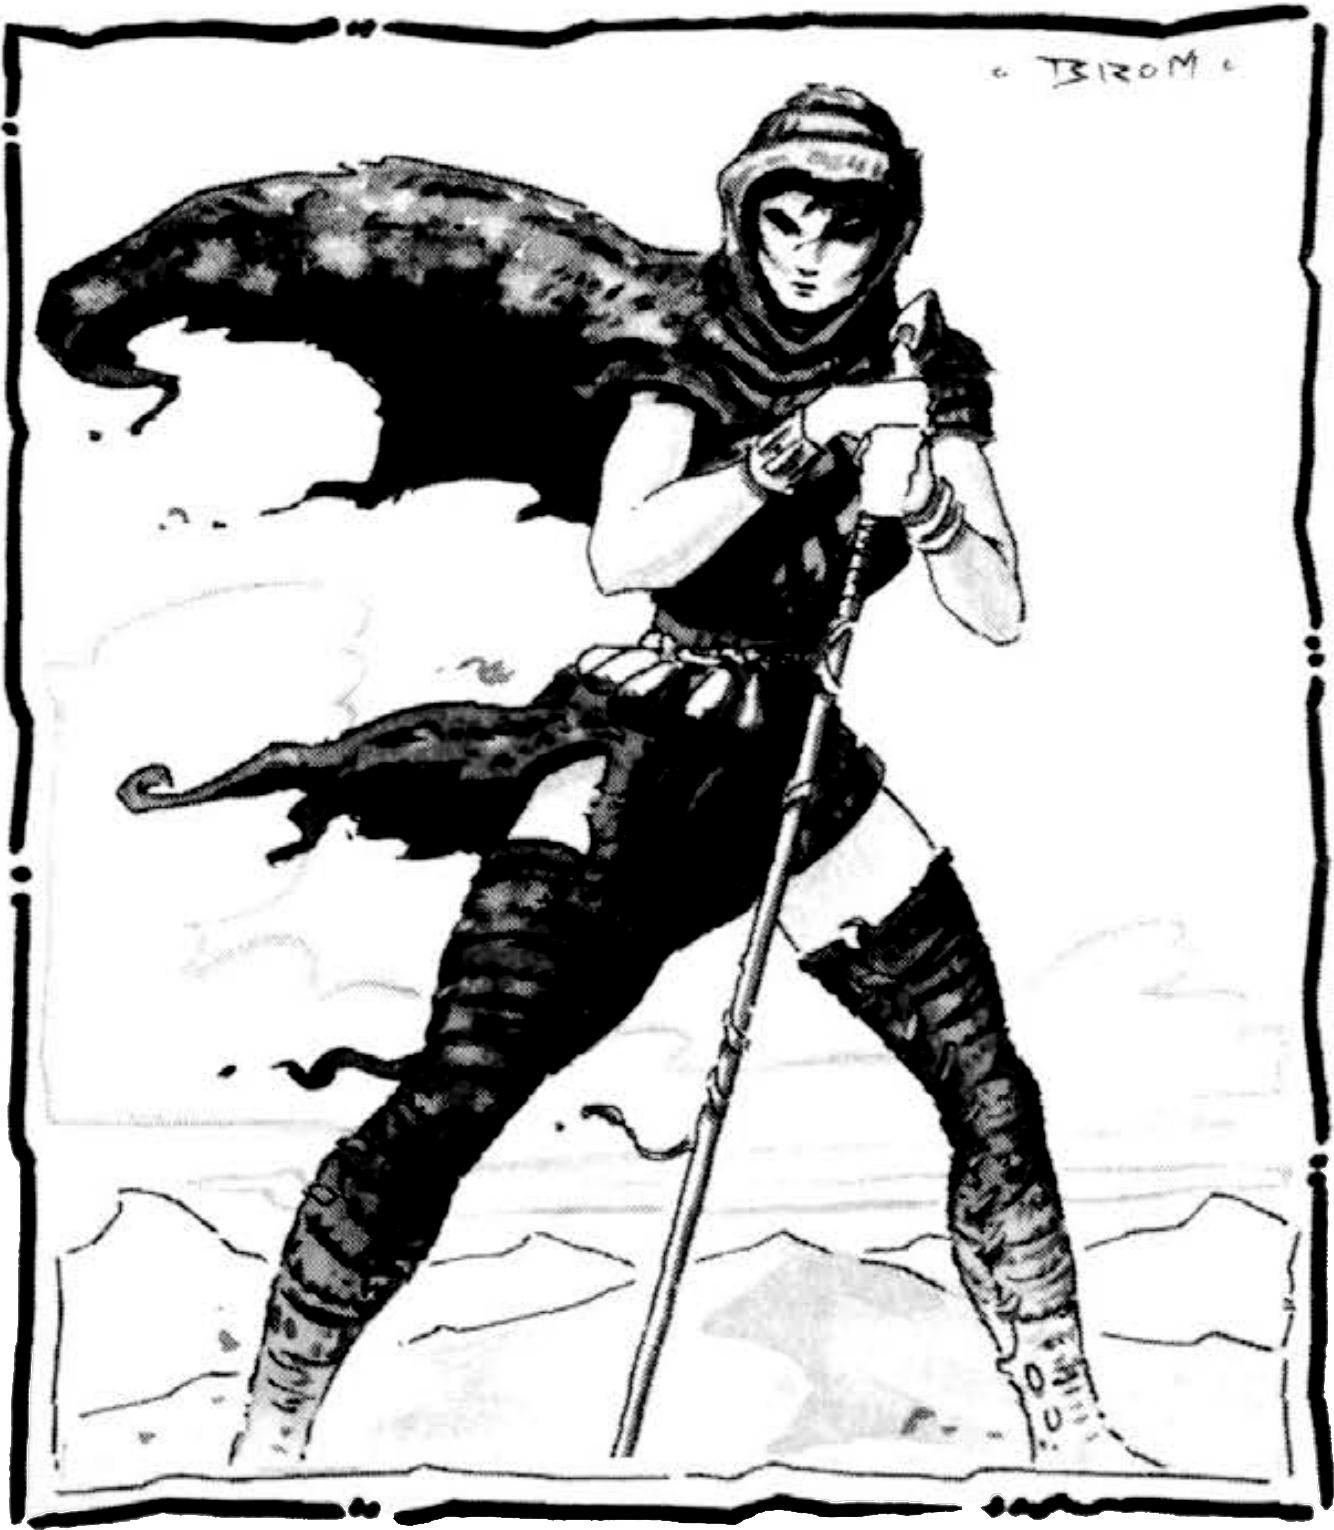
\includegraphics[width=\columnwidth]{images/halfelf-1.png}
\end{figure}
Unlike the parents of muls, elves and humans are often attracted to each other. Half-elves are typically the unwanted product of a casual interracial encounter.

\textbf{Personality:} Half-elves are notorious loners. Many Athasians believe that half-elves combine the worst traits of both races, but the most difficult aspect of half-elves---their lack of self-confidence comes not from their mixed origins but rather from a life of rejection from both parent races. Half-elves try in vain to gain the respect of humans or elves.

\textbf{Physical Description:} Averaging over 1.8 meters tall, half-elves combine Elven dexterity with human resilience. Bulkier than elves, most half-elves find it easier to pass themselves off as full humans than as full elves, but all have some features that hint at their Elven heritage.

\textbf{Relations:} Humans distrust the half-elf's Elven nature, while elves have no use for their mixed-blood children; Elven traditions demand that such children be left behind. Human society gives half-elves have a better chance of survival, but even less kindness. Half-elves sometimes find friendship among muls or even Thri-kreen. Half-elves will cooperate with companions when necessary, but find it difficult to rely on anyone. Many half-elves also turn to the animal world for company, training creatures to be servants and friends. Ironically, the survival skills and animal affinity that half-elves developed to cope with isolation make them valuable beast handlers in human society.

\textbf{Alignment:} Lawful and neutral half-elves labor for acceptance from a parent race, while chaotic ones have given up on acceptance, electing instead to reject the society that has rejected them.

\textbf{Half-Elven Lands:} Despite their unique nature, half-elves don't form communities. The few half-elves that settle down tend to live among humans who, unlike elves, at least find a use for them.

\textbf{Magic:} Half-elves often take up arcane studies, because it is a solitary calling.

\textbf{Psionics:} Mastery of the Way often provides the independence and self-knowledge that half-elves seek, and membership in a psionic academy can provide the half-elf with acceptance.

\textbf{Religion:} Because of their alienation from society and their affinity with animals, half-elves make excellent druids. Some half-elves turn their resentment of society into a profession and become sullen, bullying templars. As clerics, they are drawn to water's healing influence.

\textbf{Language:} Half-elves all speak the Common tongue. A few half-elves pick up the Elven language.

\textbf{Names:} Half-elves nearly always have human names. Unable to run as elves, they never receive Elven given names, or acceptance in an Elven tribe that they could use as surname.

\textbf{Adventurers:} In a party, half-elves often seem detached and aloof.

\subsection{Half-Elf Society}
Unlike other races, half-elves do not consider themselves a separate race, and, with very few exceptions, do not try to form half-Elven communities. A half-elf's life is typically harder than either a human's or an elf's. It is difficult for half-elves to find acceptance within either Elven or human society. Elves have not tolerance for those of mixed heritage, while humans do not trust their Elfish side. On the whole, humans are far more tolerant of half-elves than elves, who often refuse to allow such children into their tribes, and are likely to cast the half-elf's mother from the tribe as well.

Most half-elves consider themselves outsiders to all society and tend to wander throughout their entire lives, going through life as an outsider and loner. Half-elves are forced to develop a high level of self-reliance. Most half-elves take great pride in their self-reliance, but this pride often makes half-elves seem aloof to others. For many half-elves the detachment is a defensive mechanism to deal with a desire for acceptance from either human or Elven society that will likely never come. Some half-elves turn to the animal world for company, training creatures to be servants and friends.

\subsection{Roleplaying Suggestions}
Desperate for the approval of either elves or humans, you are even more desperate to appear independent and self-reliant, to cover your desire for approval. As a result, you tend towards a feisty, insecure, sullen self-reliance, refusing favors. You take every opportunity to show off your skills in front of elves and humans, but if an elf or a human were to actually praise you, you would probably react awkwardly or suspiciously. From your childhood, your closest friendships have been with animals. Other half-elves do not interest you. As time goes by and you learn from experience, you will find that you can also get along with other races neither human nor Elven: dwarves, pterran, muls, even thri-kreen. You don't feel the terrible need for their approval, and yet they give it more readily.

\subsection{Half-Elf Racial Traits}
\begin{itemize*}
    \item +2 Dexterity, $-2$ Charisma: Half-elves are limber like their Elven parents, but their upbringing leaves them with a poor sense of self, and affects their relations with others.
    \item Humanoid (elf): Half-elves are humanoid creatures with the elf subtype.
    \item Medium: As Medium creatures, half-elves have no bonuses or penalties due to size.
    \item Half-elf base land speed is 9 meters.
    \item Low-Light Vision: A half-elf can see twice as far as a human in starlight, moonlight, torchlight, and similar conditions of poor illumination. She retains the ability to distinguish color and detail under these conditions..
    \item Half-elves gain a +2 racial bonus to \skill{Disguise} checks when impersonating elves or humans.
    \item +1 racial bonus on \skill{Listen}, \skill{Search} and \skill{Spot} checks. Half-elves have keen senses, but not as keen as those of an elf.
    \item +2 racial bonus on all \skill{Survival} and \skill{Handle Animal} checks. Half-elves spend a lot of time in the wilds of the tablelands.
    \item Elven Blood: For all effects related to race, a half-elf is considered an elf. Half-elves, for example, are just as vulnerable to effects that affect elves as their elf ancestors are, and they can use magic items that are only usable by elves.
    \item Automatic Languages: Common and Elven. Bonus Languages: Any.
    \item Favored Class: Any. When determining whether a multiclass half-elf takes an experience point penalty, his highest-level class does not count when determining whether he takes an experience point for multiclassing.
\end{itemize*}
\section{Half-Giants}
\Quote{Mind of a child, strength of three grown men. I've seen a half-giant tear the walls out of a building because he wanted a better look at the tattoos on a mul inside.}{Daro, human trader}

Legend has it that in ages past, a sorcerer-queen used wizardry to beget a union of giant and human in order to create a race of powerful slaves. Whatever the truth of this legend, the half-giant race has increased in number and is now fairly common especially in human controlled lands near the shore of the Sea of Silt. Half-giants gain great strength, but dull wits, from their giant heritage, and are nearly as agile as their human forbearers.

\begin{figure}[t!]
\centering
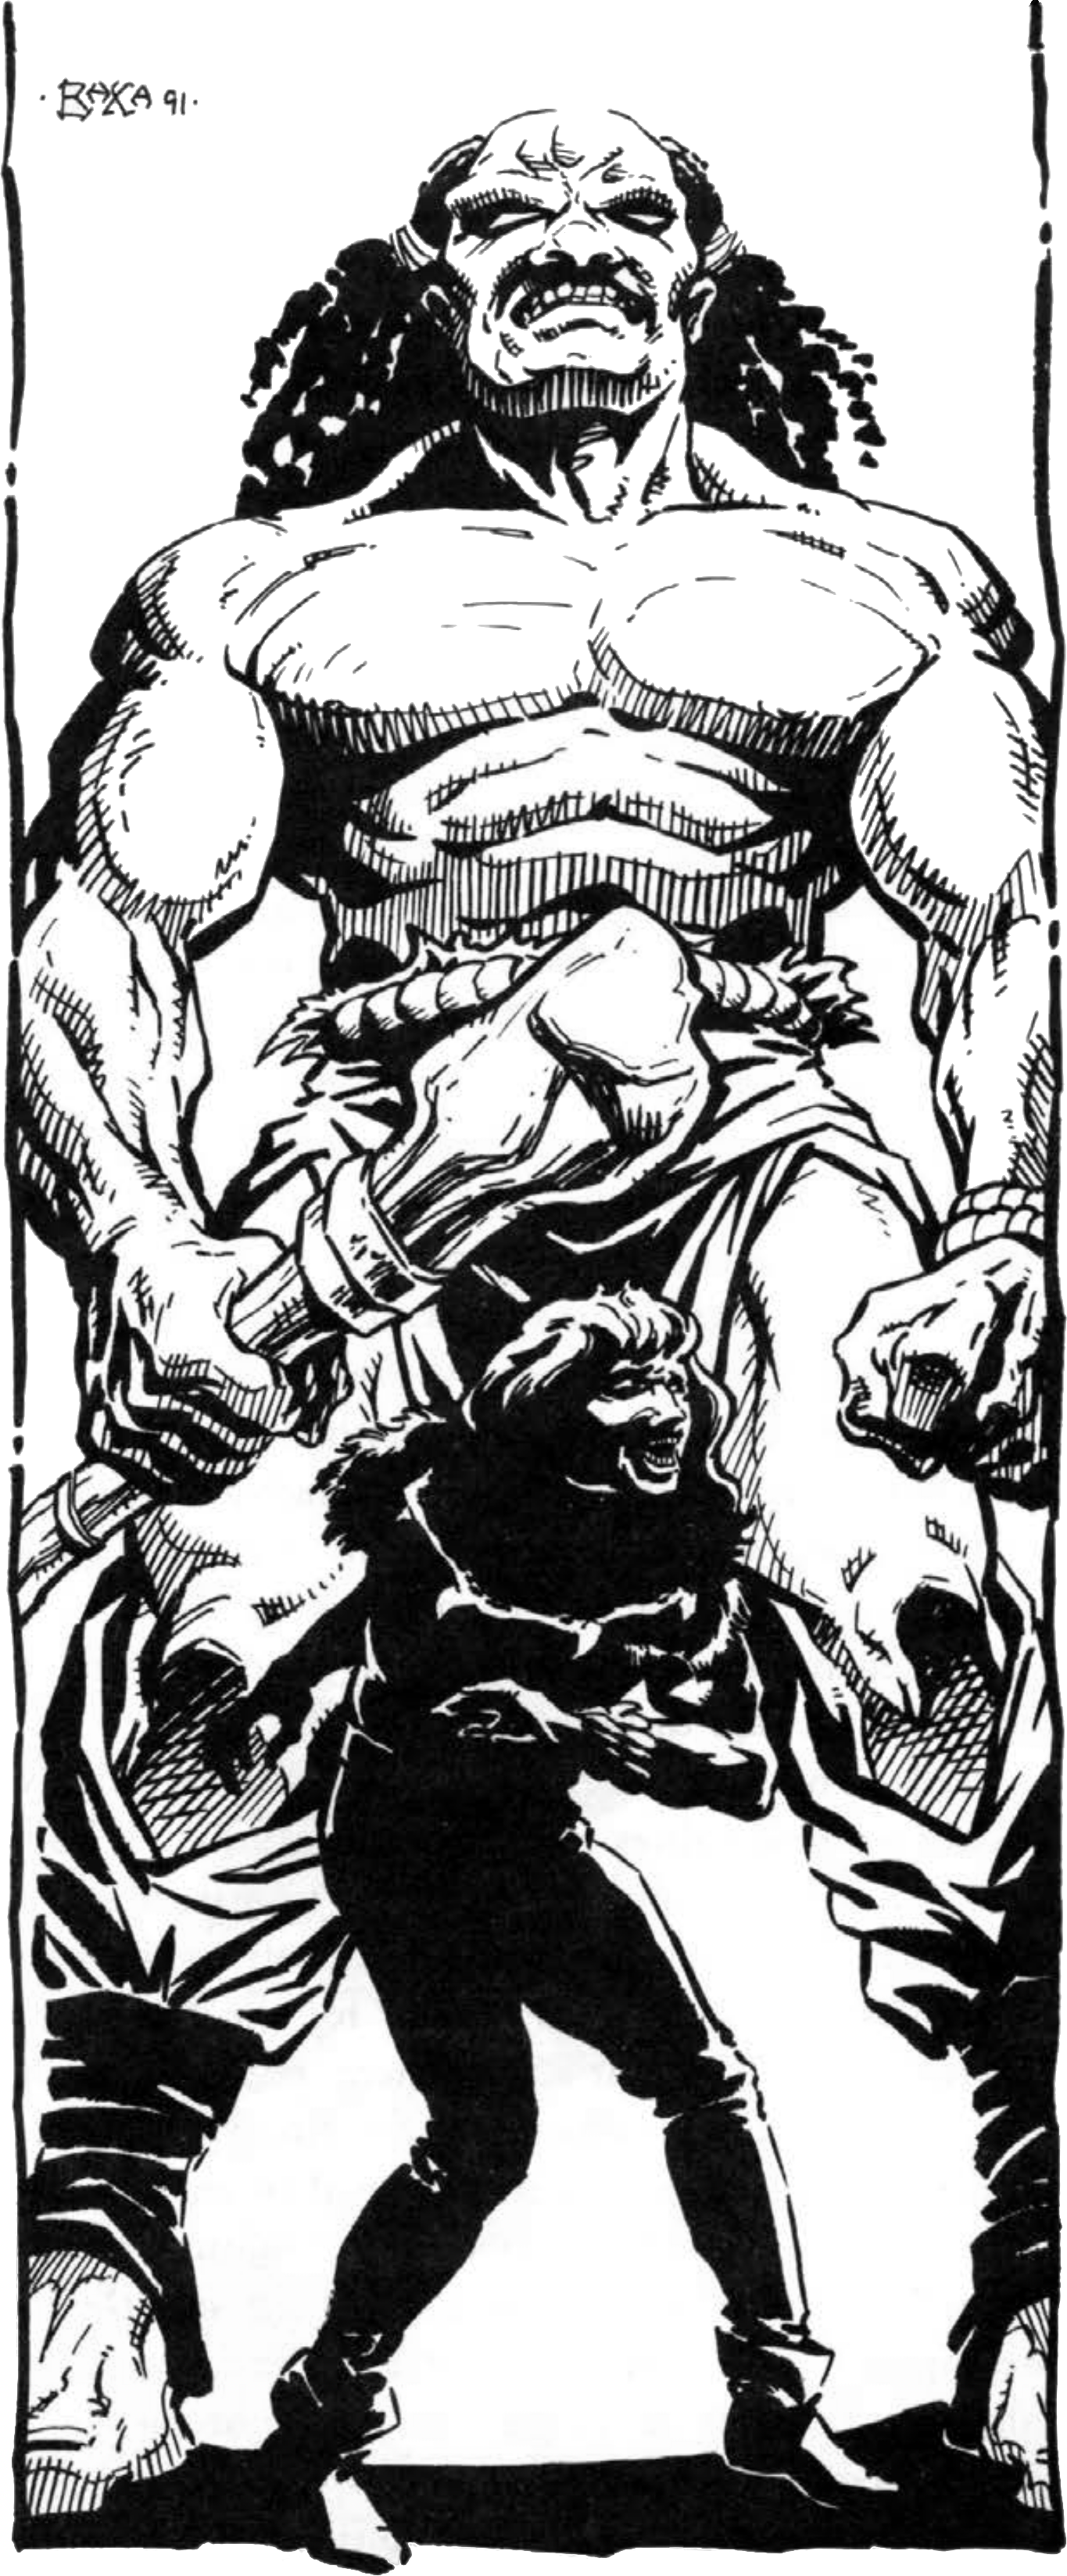
\includegraphics[width=\columnwidth]{images/halfgiant-1.png}
\WOTC
\end{figure}

\textbf{Personality:} Because of their artificial origins, there is no half-giant culture, tradition or homeland. Half-giants readily imitate the customs and cultures of their neighbors. Half-giants often display curiosity, a willingness to learn, and a general tendency towards kindness.

\textbf{Physical Description:} Physically, the half-giant is enormous, standing about 3.5 meters tall and weighing around 600 kg. Half-giants have thick hair, which is often kept braided (especially among females) or in a single tail that hangs behind the head and down the back. They dress in garb suitable to their occupation or environment. Half-giants mature at about 24 years of age and can live about 170 years.

\textbf{Relations:} The most powerful warriors on Athas, half-giants seem content to dwell in humanity's shadow. Half-giants tend to be friendly and eager to please, adopting the lifestyles, skills, and values of those they admire. A half-giant character who encounters a new situation looks around him to see what other people are doing. For example, a half-giant character that happens upon a Dwarven stone quarry may watch the dwarves, and then start quarrying stone himself. If he can make a living at it, he will continue to quarry stone just like his neighbor dwarves do; otherwise he will move on to something else.

\textbf{Alignment:} Half-giants can switch attitudes very quickly, taking on new values to fit new situations. A half-giant whose peaceful farming life is disrupted by marauders may soon adopt the morals of the renegades who sacked his village. A half-giant's nature is to switch his alignment aspect to imitate or otherwise react to a significant change around him.

\textbf{Half-Giant Lands:} Half-giants are most often found in the city-states, serving as gladiators, laborers, soldiers, and guards. A few half-giants collect into wilderness communities, often adopting the culture and customs of neighboring beings. The rare half-giant community often attaches itself to a charismatic or successful leader (not necessarily a half-giant) who demonstrates the tendencies they admire.

\textbf{Magic:} If a half-giant's companions accept wizardry, then the half-giant will also accept it. If a half-giant's companions hate wizardry, then the half-giant will be as eager as anyone to join in stoning a wizard. Among sophisticated companions who accept preserving magic but despise defiling magic, all but the brightest half-giants are likely to become confused, looking to their companions to see how they should react.

\textbf{Psionics:} While a single-classed half-giant psion is very rare, some half-giants take the path of the psychic warrior, becoming killing machines that can take apart a mekillot barehanded.

\textbf{Religion:} Half-giants do not display any affinity for the worship of one element over another.

\textbf{Language:} All half-giants speak the Common speech of slaves. Whatever tongue she speaks, the half-giant's voice is pitched so low as to occasionally be difficult to understand.

\textbf{Names:} Enslaved half-giants often have human names, and because of this they vary greatly. Free half-giants are likely to borrow the naming conventions of the race or people they are imitating at the time their child is born.

\textbf{Adventurers:} Half-giants are usually led to adventure by interesting companions of other races.

\subsection{Half-Giant Society}
A relatively young race, half-giants possess very little cultural identify of their own. Instead they adopt the customs and beliefs of those other cultures in which they live. Because of this, half-giants routinely change their alignment to match those around them who most influence them.
Half-giants can be found from one end of the Tablelands to the other, and often congregate in or near other population centers, absorbing the culture. Rarely do half-giants form communities of their own.

Unlike some other bastard races, half-giants can reproduce. A single off-spring is produced from half-giant unions after almost a year of pregnancy.

Though omnivorous, half-giants are tremendous consumers of water and food. They require twice the amount of food and water than humans. Clothing and equipment need twice the material to construct to fit a half-giant, leading to higher prices for half-giants.

Half-giants tend to damage objects and buildings around them through accidents of size alone. Some considerate half-giants camp outside city walls to avoid causing too much damage, but the draw of a city's culture and the below average intellect of most half-giants limits the number of half-giants who do so.

\subsection{Roleplaying Suggestions}
Always remember how much bigger and heavier you are than everyone else. Take advantage of your height in combat, but remember the disadvantages. Between your size and your lesser wits (even if you are a relatively intelligent half-giant people will assume you to be dull), you find yourself an object of comic relief. You are used to being teased and will endure more witty remarks than most people, but when you have been pushed too far your personality can suddenly shift, and you can unleash astonishing violence on your tormentors and any who stand in your way. Less frequently, these shifts can happen to you without provocation you just wake up with a different ethos and altered disposition.

Remember you are influenced by powerful personalities, and can shift your personality and ethics. You tend to imitate the tactics, clothes and demeanor of your ``little master.''
\subsection{Half-Giant Racial Traits}
\begin{itemize*}
    \item +8 Strength, +4 Constitution, $-2$ Dexterity, $-4$ Intelligence, $-4$ Wisdom, $-4$ Charisma: Half-giants are renowned for their great strength and dull wits.
    \item Large: As a Large creature, a half-giant takes a $-1$ penalty to Armor Class, a $-1$ penalty on attack rolls, and a $-4$ penalty on \skill{Hide} checks. She gains a +4 size bonus on grapple checks, and her lifting and carrying limits are double those of Medium characters, but she uses bigger weapons than humans use.
    \item Half-giants occupy a space of 3 meters and have a reach of 3 meters.
    \item Giant: Half-giants are creatures with the giant type.
    \item Half-giant base land speed is 12 meters.
    \item Darkvision: Half-giants can see in the dark out to 18 meters. Darkvision is black and white only, but it is otherwise like normal sight, and half-giants can function just fine with no light at all.
    \item Natural Armor: Half-giants have a +2 natural armor bonus to AC.
    \item Axis Alignment: One aspect of the half-giant's alignment must be fixed, and chosen during character creation. The other half must be chosen when they awake each morning. They are only bound to that alignment until they sleep again. For example, a half-giant may have a fixed lawful alignment. Every morning, he must choose to be lawful good, lawful neutral or lawful evil. This alignment change is not mandatory.
    \item Half-giants consume double the amount of food and water humans do.
    \item Favored Class: Barbarian. A multiclass half-giant's barbarian class does not count when determining whether he takes an experience point for multiclassing.
    \item Automatic Languages: Common. Bonus Languages: Dwarven, Gith, Giant. Half-giants will often pick up a race's tongue if imitating them long enough.
    \item Level Adjustment: +2. Half-giants are more powerful than the other races of the Tablelands and gain levels accordingly.
\end{itemize*}
\begin{figure*}[b!]
\centering
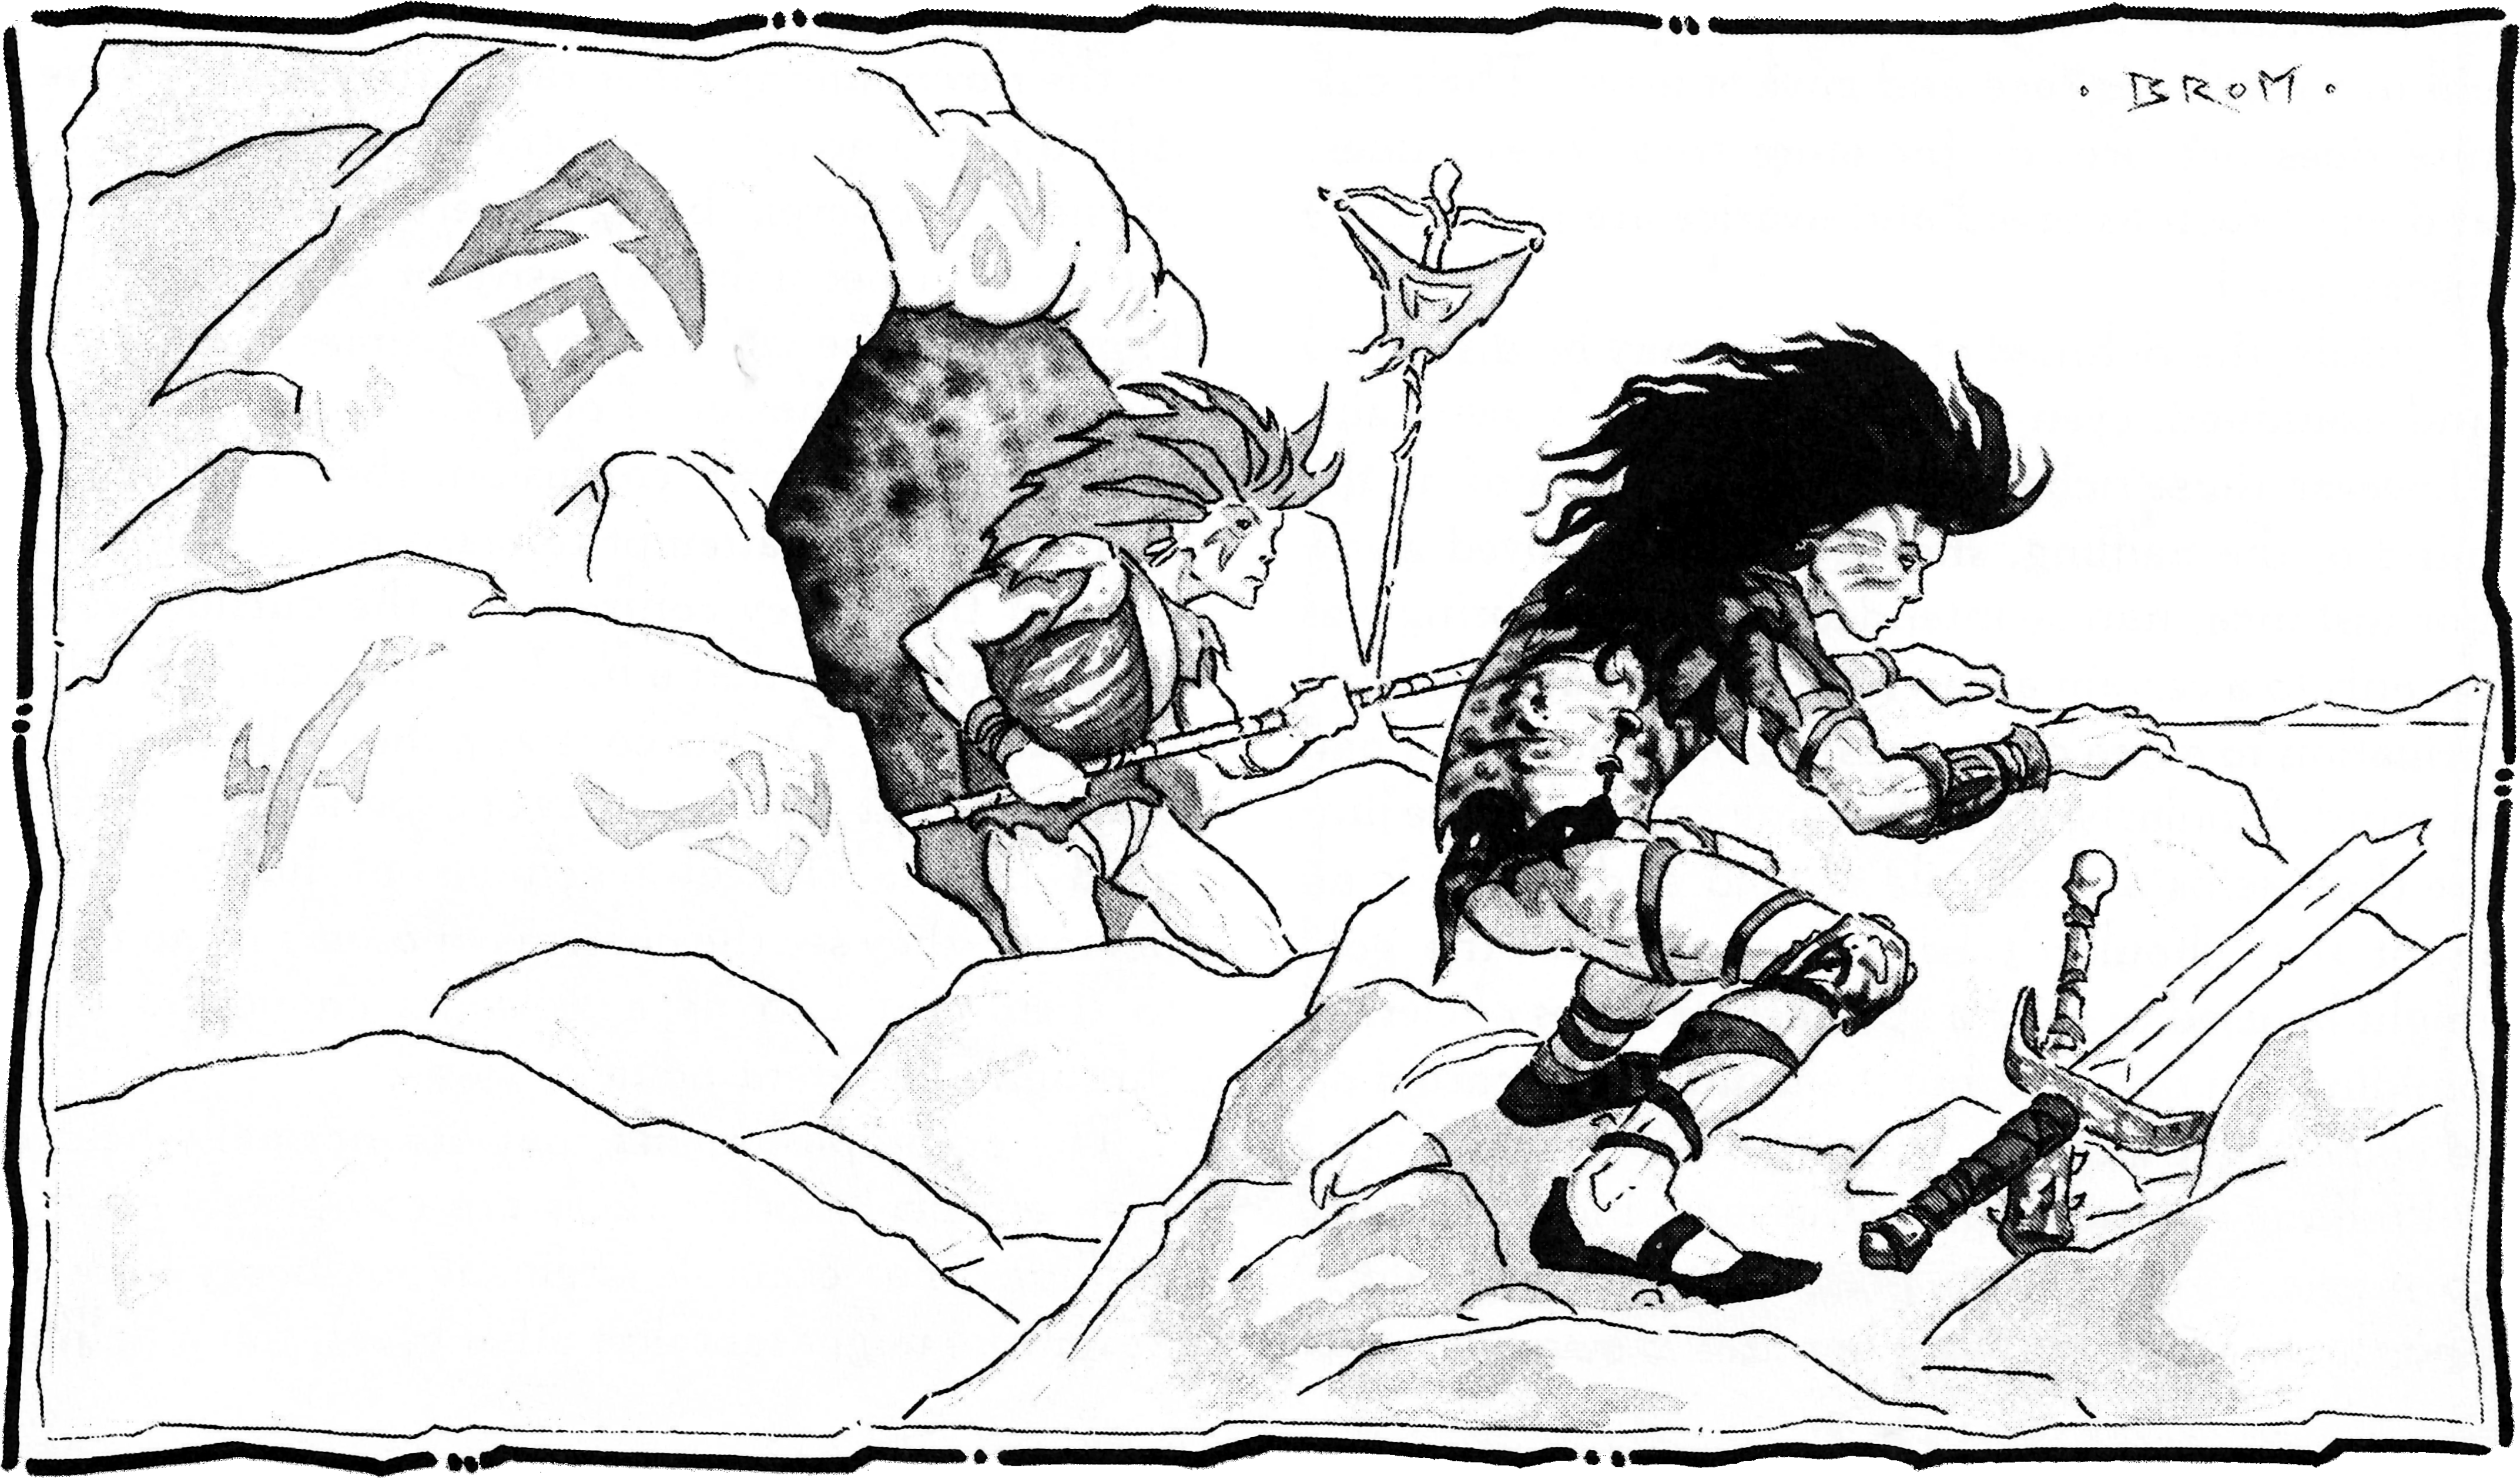
\includegraphics[width=\textwidth]{images/halfling-2.png}
\WOTC
\end{figure*}

\section{Halflings}
\Quote{Be wary of the forest ridge. The halflings who live there would as soon eat you alive as look at you. Chances are you won't even notice them until you've become the main course.}{Mo'rune, half-Elven ranger}

Halflings are masters of the jungles of the Ringing Mountains. They are small, quick and agile creatures steeped in an ancient and rich culture that goes back far into Athas' past. Although they are not common in the Tablelands, some halflings leave their homes in the forests to adventure under the{\tableheader Dark Sun}. As carnivores, halflings prefer to eat flesh raw.

\textbf{Personality:} Halflings have difficulty understanding others' customs or points of view, but curiosity helps some halflings overcome their xenophobia. Little concerned with material wealth, halflings are more concerned with how their actions will affect other halflings.

\textbf{Physical Description:} Halflings are small creatures, standing only about 1 meter tall and weighing 25 to 30 kilograms. Rarely affected by age, halfling faces are often mistaken for the faces of human children. They dress in loincloths, sometimes with a shirt or vest, and paint their skins with bright reds and greens. Forest halflings rarely tend to their hair, and some let it grow to great lengths, though it can be unkempt and dirty. They live to be about 120 years old.

\textbf{Relations:} Halfling's culture dominates their relations with others. They relate very well to each other, since they all have the same cultural traits and are able to understand each other. Halflings of different tribes still share a tradition of song, art and poetry, which serves as a basis of communication. Creatures that do not know these cultural expressions are often at a loss to understand the halfling's expressions, analogies and allusions to well-known halfling stories. Halflings can easily become frustrated with such ``uncultured'' creatures. They abhor slavery and most halflings will starve themselves rather than accept slavery.

\textbf{Alignment:} Halflings tend towards law and evil. Uncomfortable with change, halflings tend to rely on intangible constants, such as racial identity, family, clan ties and personal honor. On the other hand, halflings have little respect for the laws of the big people.

\textbf{Halfling Lands:} Halflings villages are rare in the tablelands. Most halflings live in tribes or clans in the Forest Ridge, or in the Rohorind forest west of Kurn. Many dwell in treetop villages. Non-halflings typically only see these villages from within a halfling cooking pot.

\textbf{Magic:} Many halfling tribes reject arcane magic. Tribes that accept wizards tend to have preserver chieftains. Only renegade halfling tribes are ever known to harbor defilers.

\textbf{Psionics:} Many halflings become seers or nomads. In the forest ridge, many tribal halflings become multiclassed seer/rangers, and become some of the deadliest trackers on Athas.

\textbf{Religion:} Halflings' bond with nature extends into most aspects of their culture. A shaman or witch doctor, who also acts as a spiritual leader, often rules their clans. This leader is obeyed without question. Halfling fighters willingly sacrifice themselves to obey their leader.

\textbf{Language:} Halflings rarely teach others their language, but some individuals of the Tablelands have learned the wild speech. Halflings found in the Tablelands often learn to speak Common.

\textbf{Names:} Halflings tend to have only one given name.

\textbf{Male Names:} Basha, Cerk, Derlan, Drassu, Entrok, Kakzim, Lokee, Nok, Pauk, Plool, Sala, Tanuka, Ukos, Zol.

\textbf{Female Names:} Alansa, Anezka, Dokala, Grelzen, Horga, Jikx, Joura, Nasaha, Vensa.

\textbf{Adventurers:} Exploring the Tablelands gives curious halflings the opportunity to learn other customs. Although they may at first have difficulty in understanding the numerous practices of the races of the Tablelands, their natural curiosity enables them to learn and interact with others. Other halflings may be criminals, renegades or other tribal outcasts, venturing into the Tablelands to escape persecution by other halflings.

\subsection{Halfling Society}
Most halflings have a common outlook on life that results in considerable racial unity across tribal and regional ties. Rarely will one halfling draw the blood of another even during extreme disagreements. Only renegade halflings do not share this racial unity, and are cast out of their tribes because of it.

Halfling society is difficult for other races to understand, as such concepts as conquest and plundering have no place. The most important value in halfling society is the abilities of the inner self as it harmonizes with the environment and the rest of the halfling race.

Halflings are extremely conscious of their environment. They are sickened by the ruined landscape of the Tyr region and desperately try to avoid having similar devastation occur to their homelands in the Forest Ridge. Most halflings believe that care must be taken to understand and respect nature and what it means to all life on Athas.

Halfling culture is expressed richly through art and song. Story telling in which oral history is passed on to the next generation is an important part of each halfling community. Halflings rely on this shared culture to express abstract thoughts and complicated concepts. This causes problems and frustration when dealing with non-halflings. Typically halflings assume that whomever they are talking to have the same cultural background to draw upon, and find it difficult to compensate for a listener who is not intimately familiar with the halfling history and ``lacks culture.''

Generally open-minded, wandering halflings are curious about outside societies and will attempt to learn all they can about other cultures. Never, will they adopt aspects of those cultures as their own, believing halfling culture to be innately superior to all others. Nor do they seek to change others' culture or views.

While halflings are omnivorous, they vastly prefer meat. Their meat heavy diet means that halflings view all living creatures, both humanoid and animal, as more food than equals. At the same time, most halflings believe that other races have the same perception of them. As a result, halflings are rarely likely to trust another member of any other race.

\subsection{Roleplaying Suggestions}
Remember to consistently take your height into account. Roleplay the halfling culture described above: eating opponents, treating fellow halflings with trust and kindness, suspicion of big people, and general lack of interest in money.

\subsection{Halfling Racial Traits}
\begin{itemize*}
    \item $-4$ Strength, +4 Dexterity, +4 Wisdom, $-2$ Charisma: Halflings are quick and stealthy, but weaker than humans.
    \item Humanoid (halfling): Halflings are humanoid creatures with the halfling subtype.
    \item Small: As a Small creature, a halfling gains a +1 size bonus to Armor Class, a +1 size bonus on attack rolls, and a +4 size bonus on \skill{Hide} checks, but she uses smaller weapons than humans use, and her lifting and carrying limits are three-quarters of those of a Medium character.%Halflings gain a +1 size bonus to Armor Class and a +1 size bonus on all attack rolls.
    \item Halfling base land speed is 6 meters.
    % \item Halflings receive a $-2$ penalty to all \skill{Diplomacy} skill checks when dealing with other races.
    \item +4 racial bonus on \skill{Climb} and \skill{Jump} checks: Halflings are agile.
    \item +2 racial bonus on saving throws against spells and spell-like effects.
    \item +1 racial attack bonus with a thrown weapon: javelins and slings are common weapons in feral halfling society, and many halflings are taught to throw at an early age.
    \item Halflings get advantage on \skill{Listen} checks---they have keen ears. Their senses of smell and taste are equally keen; they get advantage to all Wisdom checks that assess smell or taste.
    \item Halfings consume half the amount of food and water humans do.
    \item Automatic Languages: Halfling. Bonus Languages: Common, Dwarven, Elven, Gith, Kreen, Rhul-thaun, Sylvan, and Yuan-ti.
    \item Favored Class: Druid, Ranger, or Rogue. A halfling must choose between druid, ranger, or rogue as favored class. This choice cannot be changed. A multiclass halfling's chosen class does not count when determining whether he takes an experience point for multiclassing.
    \item Level Adjustment: +1.
\end{itemize*}
\section{Muls}
\Quote{See, the trick is to break their will. Not too much, mind you. Nobody wants to watch a docile gladiator, and muls are too expensive to waste as labor slaves. But, you don't want them trying to escape every other day. Would you like to tell the arena crowd that their favorite champion will not be appearing in today's match because he died trying to escape your pens?}{Gaal, Urikite arena trainer}

Born from the unlikely parentage of dwarves and humans, muls combine the height and adaptable nature of humans with the musculature and resilience of dwarves. Muls enjoy traits that are uniquely their own, such as their robust metabolism and almost inexhaustible capacity for work. The hybrid has disadvantages in a few areas as well: sterility, and the social repercussions of being created for a life of slavery. Humans and dwarves are not typically attracted to each other. The only reason that muls are so common in the Tablelands is because of their value as laborers and gladiators: slave-sellers force-breed humans and dwarves for profit. While mul-breeding practices are exorbitantly lucrative, they are often lethal to both the mother and the baby. Conception is difficult and impractical, often taking months to achieve. Even once conceived, the mul takes a full twelve months to carry to term; fatalities during this period are high. As likely as not, anxious overseers cut muls from the dying bodies of their mothers.

\textbf{Personality:} All gladiators who perform well in the arenas receive some degree of pampered treatment, but muls receive more pampering than others. Some mul gladiators even come to see slavery as an acceptable part of their lives. However, those that acquire a taste of freedom will fight for it. Stoic and dull to pain, muls are not easily intimidated by the lash. Masters are loath to slay or maim a mul who tries repeatedly to escape, although those who help the mul's escape will be tormented in order to punish the mul without damaging valuable property. Once a mul escapes or earns his freedom, slavery remains a dominant part of his life. Most muls are heavily marked with tattoos that mark his ownership, history, capabilities and disciplinary measures. Even untattooed muls are marked as a potential windfall for slavers: it is clearly cheaper to ``retrieve'' a mul who slavers can claim had run away, than to start from scratch in the breeding pits.

\begin{figure}[t!]
\centering
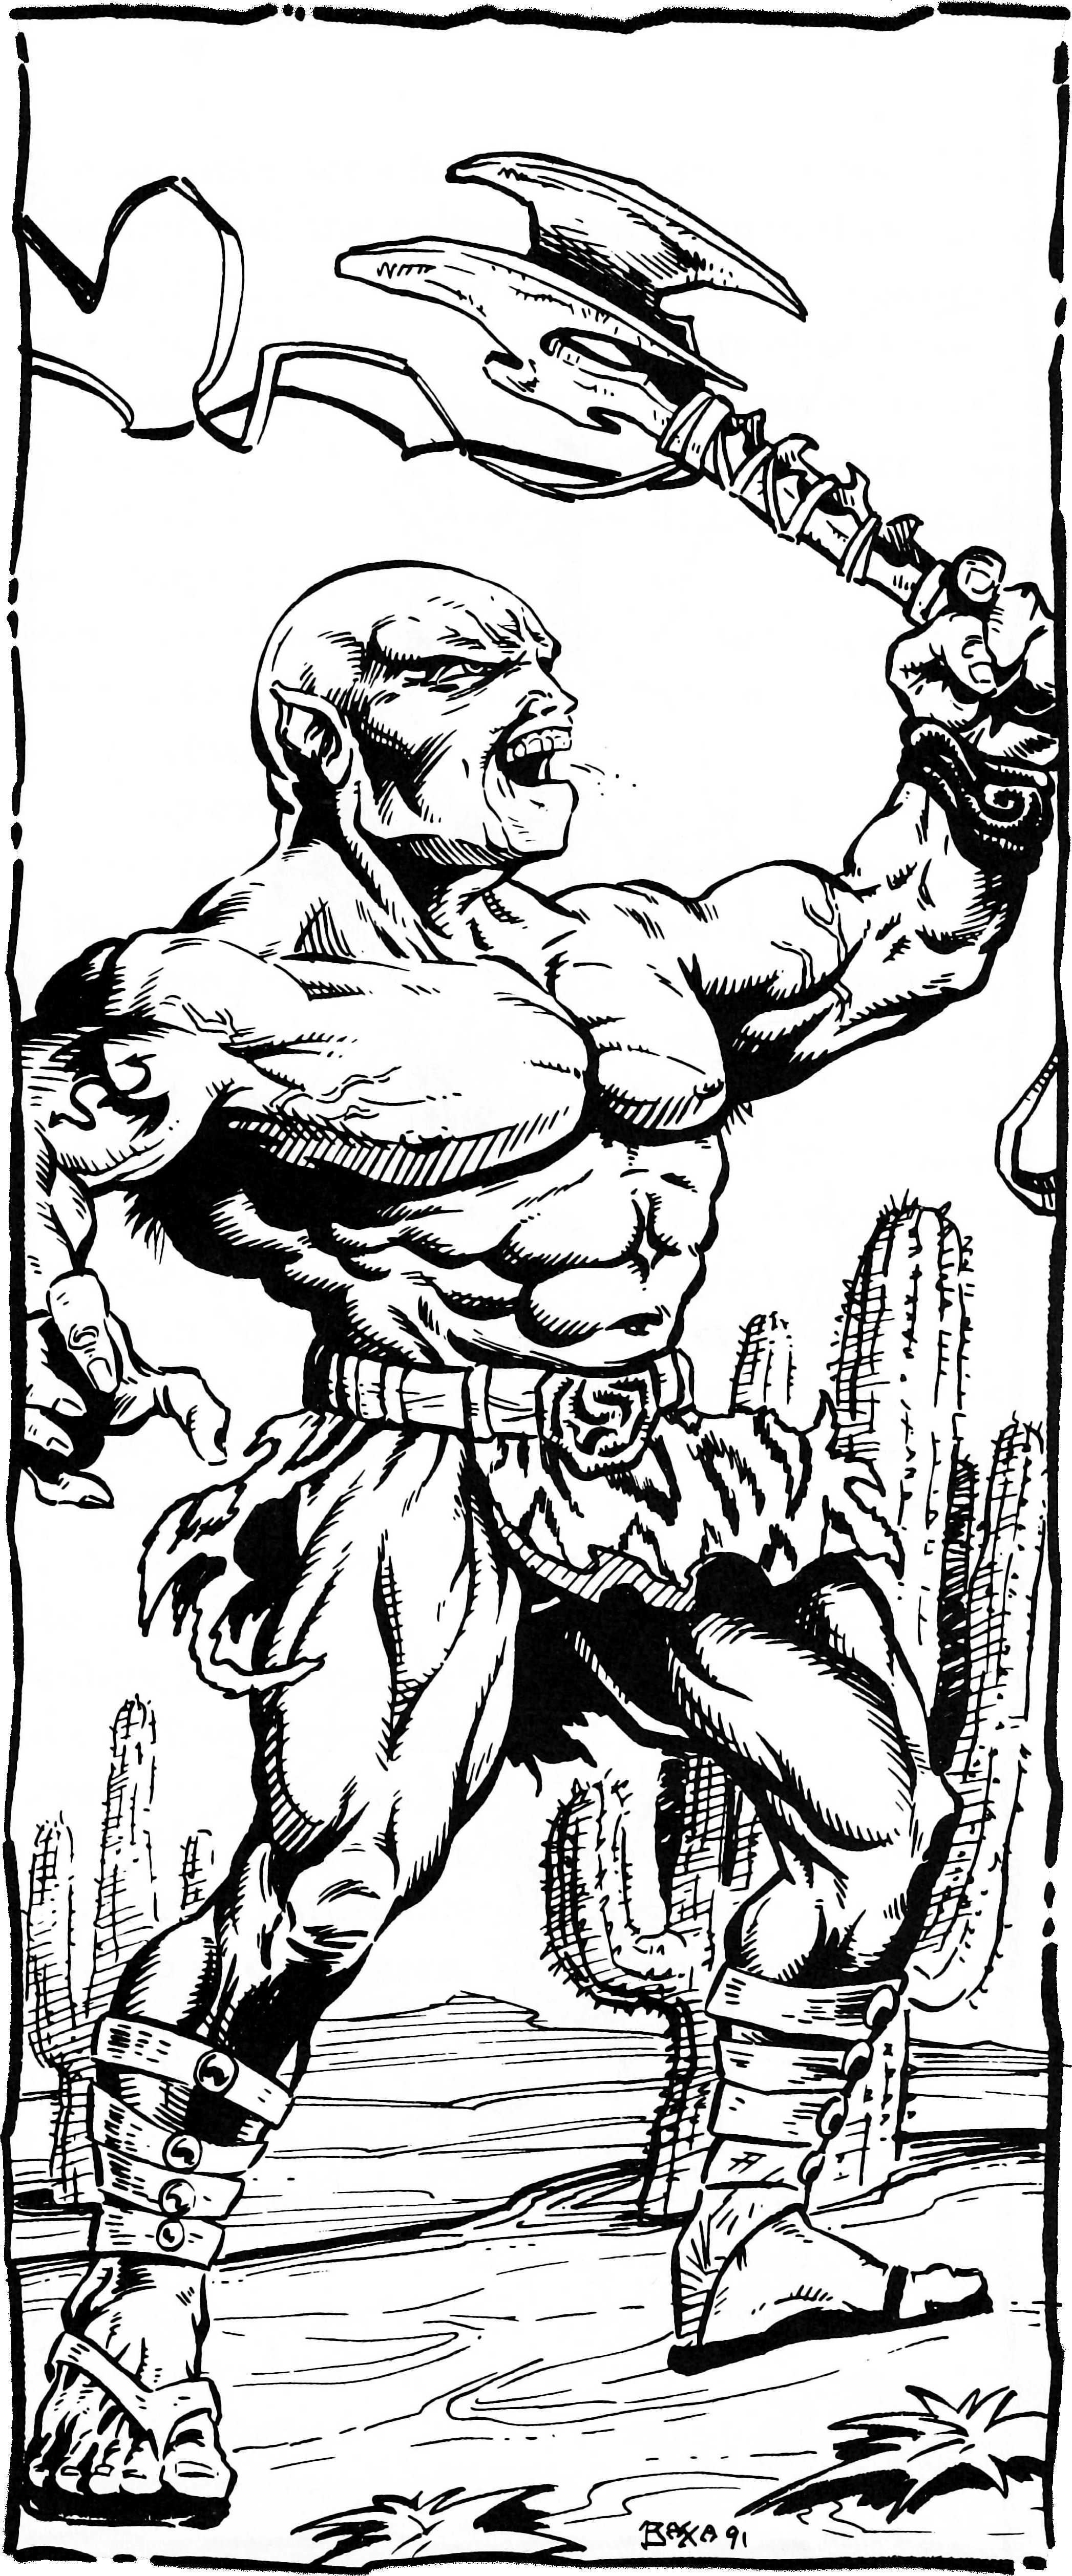
\includegraphics[width=\columnwidth]{images/mul-1.png}
\WOTC
\end{figure}

\textbf{Physical Description:} Second only to the half-giant, the mul is the strongest of the common humanoid races of the tablelands. Muls grow as high as 2.1 meters, weighing upwards of 125 kilograms, but carry almost no fat at all on their broad muscular frames. Universal mul characteristics include angular, almost protrusive eye ridges, and ears that point sharply backwards against the temples. Most muls have dark copper-colored skin and hairless bodies.

\textbf{Relations:} Most mul laborers master the conventions of slave life, figuring out through painful experience who can be trusted and who cannot. (Muls learn from their mistakes in the slave pits to a greater extent than other races not because they are cleverer, but because unlike slaves of other races they tend to survive their mistakes, while other slave races are less expensive and therefore disposable. Only the most foolish and disobedient mul would be killed. Most masters will sell a problem mul slave rather than kill him.) Their mastery of the rules of slave life and their boundless capacity for hard work allows them to gain favor with their masters and reputation among their fellow slaves.

\textbf{Alignment:} Muls tend towards neutrality with respect to good and evil, but run the gamut with respect to law or chaos. Many lawful muls adapt well to the indignities of slavery, playing the game for the comforts that they can win as valued slaves. A few ambitious lawful muls use the respect won from their fellow-slaves to organize rebellions and strike out for freedom. Chaotic muls, on the other hand, push their luck and their value as slaves to the breaking point, defying authority, holding little fear for the lash.

\textbf{Mul Lands:} As a collective group, muls have no lands to call their own. Occasionally, escaped muls band together as outlaws and fugitives, because of their common ex-slave backgrounds, and because their mul metabolism makes it easier for them to survive as fugitives while other races cannot keep up. Almost without exception, muls are born in the slave pits of the merchants and nobles of the city-states. Most are set to work as laborers, some as gladiators, and fewer yet as soldier-slaves. Very few earn their freedom, a greater number escape to freedom among the tribes of ex-slave that inhabit the wastes.

\textbf{Magic:} Muls dislike what they fear, and they fear wizards. They also resent that a wizard's power comes from without, with no seeming effort on the wizard's part, while the mul's power is born of pain and labor. Mul wizards are unheard of.

\textbf{Psionics:} Since most slave owners take steps to ensure that their property does not get schooled in the Way, it is rare for a mul to receive any formal training. Those that get this training tend to excel in psychometabolic powers.

\textbf{Religion:} Even if muls were to create a religion of their own, as sterile hybrids, they would have no posterity to pass it on to. Some cities accept muls as templars. Mul clerics tend to be drawn towards the strength of elemental earth.

\textbf{Language:} Muls speak the Common tongue of slaves, but those favored muls that stay in one city long enough before being sold to the next, sometimes pick up the city language. Because of their tireless metabolism, muls have the capacity to integrate with peoples that other races could not dream of living with, such as elves and Thri-kreen.

\textbf{Names:} Muls sold as laborers will have common slave names. Muls sold as gladiators will often be given more striking and exotic names. Draji names (such as Atlalak) are often popular for gladiators, because of the Draji reputation for violence. Masters who change their mul slaves' professions usually change their names as well, since it is considered bad form to have a gladiator with a farmer's name, and a dangerous incitement of slave rebellions to give a common laborer the name of a gladiator.

\textbf{Adventurers:} Player character muls are assumed to have already won their freedom. Most freed mul gladiators take advantage of their combat skills, working as soldiers or guards. Some turn to crime, adding rogue skills to their repertoire. A few muls follow other paths, such as psionics, templar orders or elemental priesthoods.

\subsection{Mul Society}
Muls have no racial history or a separate culture. They are sterile and cannot reproduce, preventing them from forming family groups and clans. The vast majority of muls are born in slavery, through breeding programs. Often the parents resent their roles in the breeding program and shun the child, leaving the mul to a lonely, hard existence. The taskmaster's whip takes the place of a family. For these reasons, many muls never seek friends or companionship, and often have rough personalities with tendencies towards violence.

The mul slave trade is very profitable, and thus the breeding programs continue. A slave trader can make as much on the sale of a mul as he could with a dozen humans. As slaves, a mul has his profession selected for him and is given extensive training as he grows.

Mul gladiators are often very successful, and win a lot of money for their owners. Highly successful gladiators are looked after by their owners, receiving a large retinue of other slaves to tend to their whims and needs. This has lead to the expression, ``pampered like a mul,'' being used often by the common folk.

Muls not trained as gladiators are often assigned to hard labor and other duties that can take advantage of the mul's hardy constitution and endurance.

\subsection{Roleplaying Suggestions}
Born to the slave pens, you never knew love or affection; the taskmaster's whip took the place of loving parents. As far as you have seen, all of life's problems that can be solved are solved by sheer brute force. You know to bow to force when you see it, especially the veiled force of wealth, power and privilege. The noble and templar may not look strong, but they can kill a man with a word. You tend towards gruffness. In the slave pits, you knew some muls that never sought friends or companionship, but lived in bitter, isolated servitude. You knew other muls who found friendship in an arena partner or co-worker. You are capable of affection, trust and friendship, but camaraderie is easier for you to understand and express - warriors slap each other on the shoulder after a victory, or give their lives for each other in battle. You don't think of that sort of event as ``friendship'' - it just happens.

\subsection{Mul Racial Traits}
\begin{itemize*}
    \item +4 Strength, +2 Constitution, $-2$ Intelligence, $-4$ Charisma: Combining the human height with the Dwarven musculature, muls end up stronger than either parent race, but their status as born-to-be slaves makes them insecure in their dealings with others.
    \item Humanoid (dwarf): Muls are humanoid creatures with the dwarf subtype.
    \item Medium: As Medium creatures, muls have no bonuses or penalties due to size.
    \item Mul base land speed is 9 meters.
    % \item Darkvision: Muls can see in the dark up to 9 meters. Darkvision is black and white only, but is otherwise like normal sight, and muls can function just fine with no light at all.
    \item Muls have +2 racial bonus on his damage rolls with light or thrown weapons (including unarmed strikes).
    \item Extended Activity: Muls require double the amount of time before making any check related to endurance.
    \begin{itemize*}
        \item Muls need to sleep every two days (but may choose to sleep every day);
        \item Muls can walk for 16 hours before beginning a forced march;
        \item Muls can hold their breath or run for a number of rounds equal to four times their Constitution score;
        \item Muls can go without food for six days;
        \item Muls can go without water for two days plus a number of hours equal to twice their Constitution score;
        \item Muls make Constitution checks every two hours of marching beyond 16 hours;
        \item Muls make Constitution checks every two rounds to continue holding their breath or running;
        \item Muls make Fortitude checks every two hours in a very hot (32 °C to 42 °C) or very cold ($-17$ °C to 4 °C) environments, every 20 minutes in severe heat (43 °C to 60 °C) or severe cold ($-28$ °C to $-18$ °C), and every 10 minutes in extreme heat \hskip10cm (61 °C to 82 °C), extreme cold ($-45$ °C to $-29$ °C), or worse environments;
        \item Muls make Constitution checks every two days after the first period without food;
        \item Muls make Constitution checks every two hours after the first period without water.
    \end{itemize*}
    % \item Tireless: Muls get a +4 racial bonus to checks for performing a physical action that extends over a period of time (running, swimming, holding breath, and so on). This bonus stacks with the \feat{Endurance} feat. This bonus may also be applied to savings throws against spells and magical effects that cause weakness, fatigue, exhaustion or enfeeblement.
    % \item Extended Activity: Muls may engage in up to 12 hours of hard labor or forced marching without suffering from the associated nonlethal damage and fatigue.
    \item Dwarven Blood: For all effects related to race, a mul is considered a dwarf. Muls, for example, are just as vulnerable to effects that affect dwarves as their dwarf ancestors are, and they can use magic items that are only usable by dwarves.
    % \item Nonlethal Damage Resistance 1/--. Muls are difficult to subdue, and do not notice minor bruises, scrapes, and other discomforts that pain creatures of other races.
    \item Favored Class: Fighter or Gladiator. A mul must choose between fighter or gladiator as favored class. This choice cannot be changed. A multiclass mul's chosen class does not count when determining whether he takes an experience point for multiclassing.
    \item Automatic Language: Common. Bonus Languages: Dwarven, Elven, Gith, and Giant.
    \item Level Adjustment: +1.
\end{itemize*}
\section{Pterrans}
\Quote{The people of the Tablelands know nothing of life. They choose no Path for themselves, and consume everything until they are dead.}{Keltruch, pterran ranger}

\begin{figure}[b!]
\centering
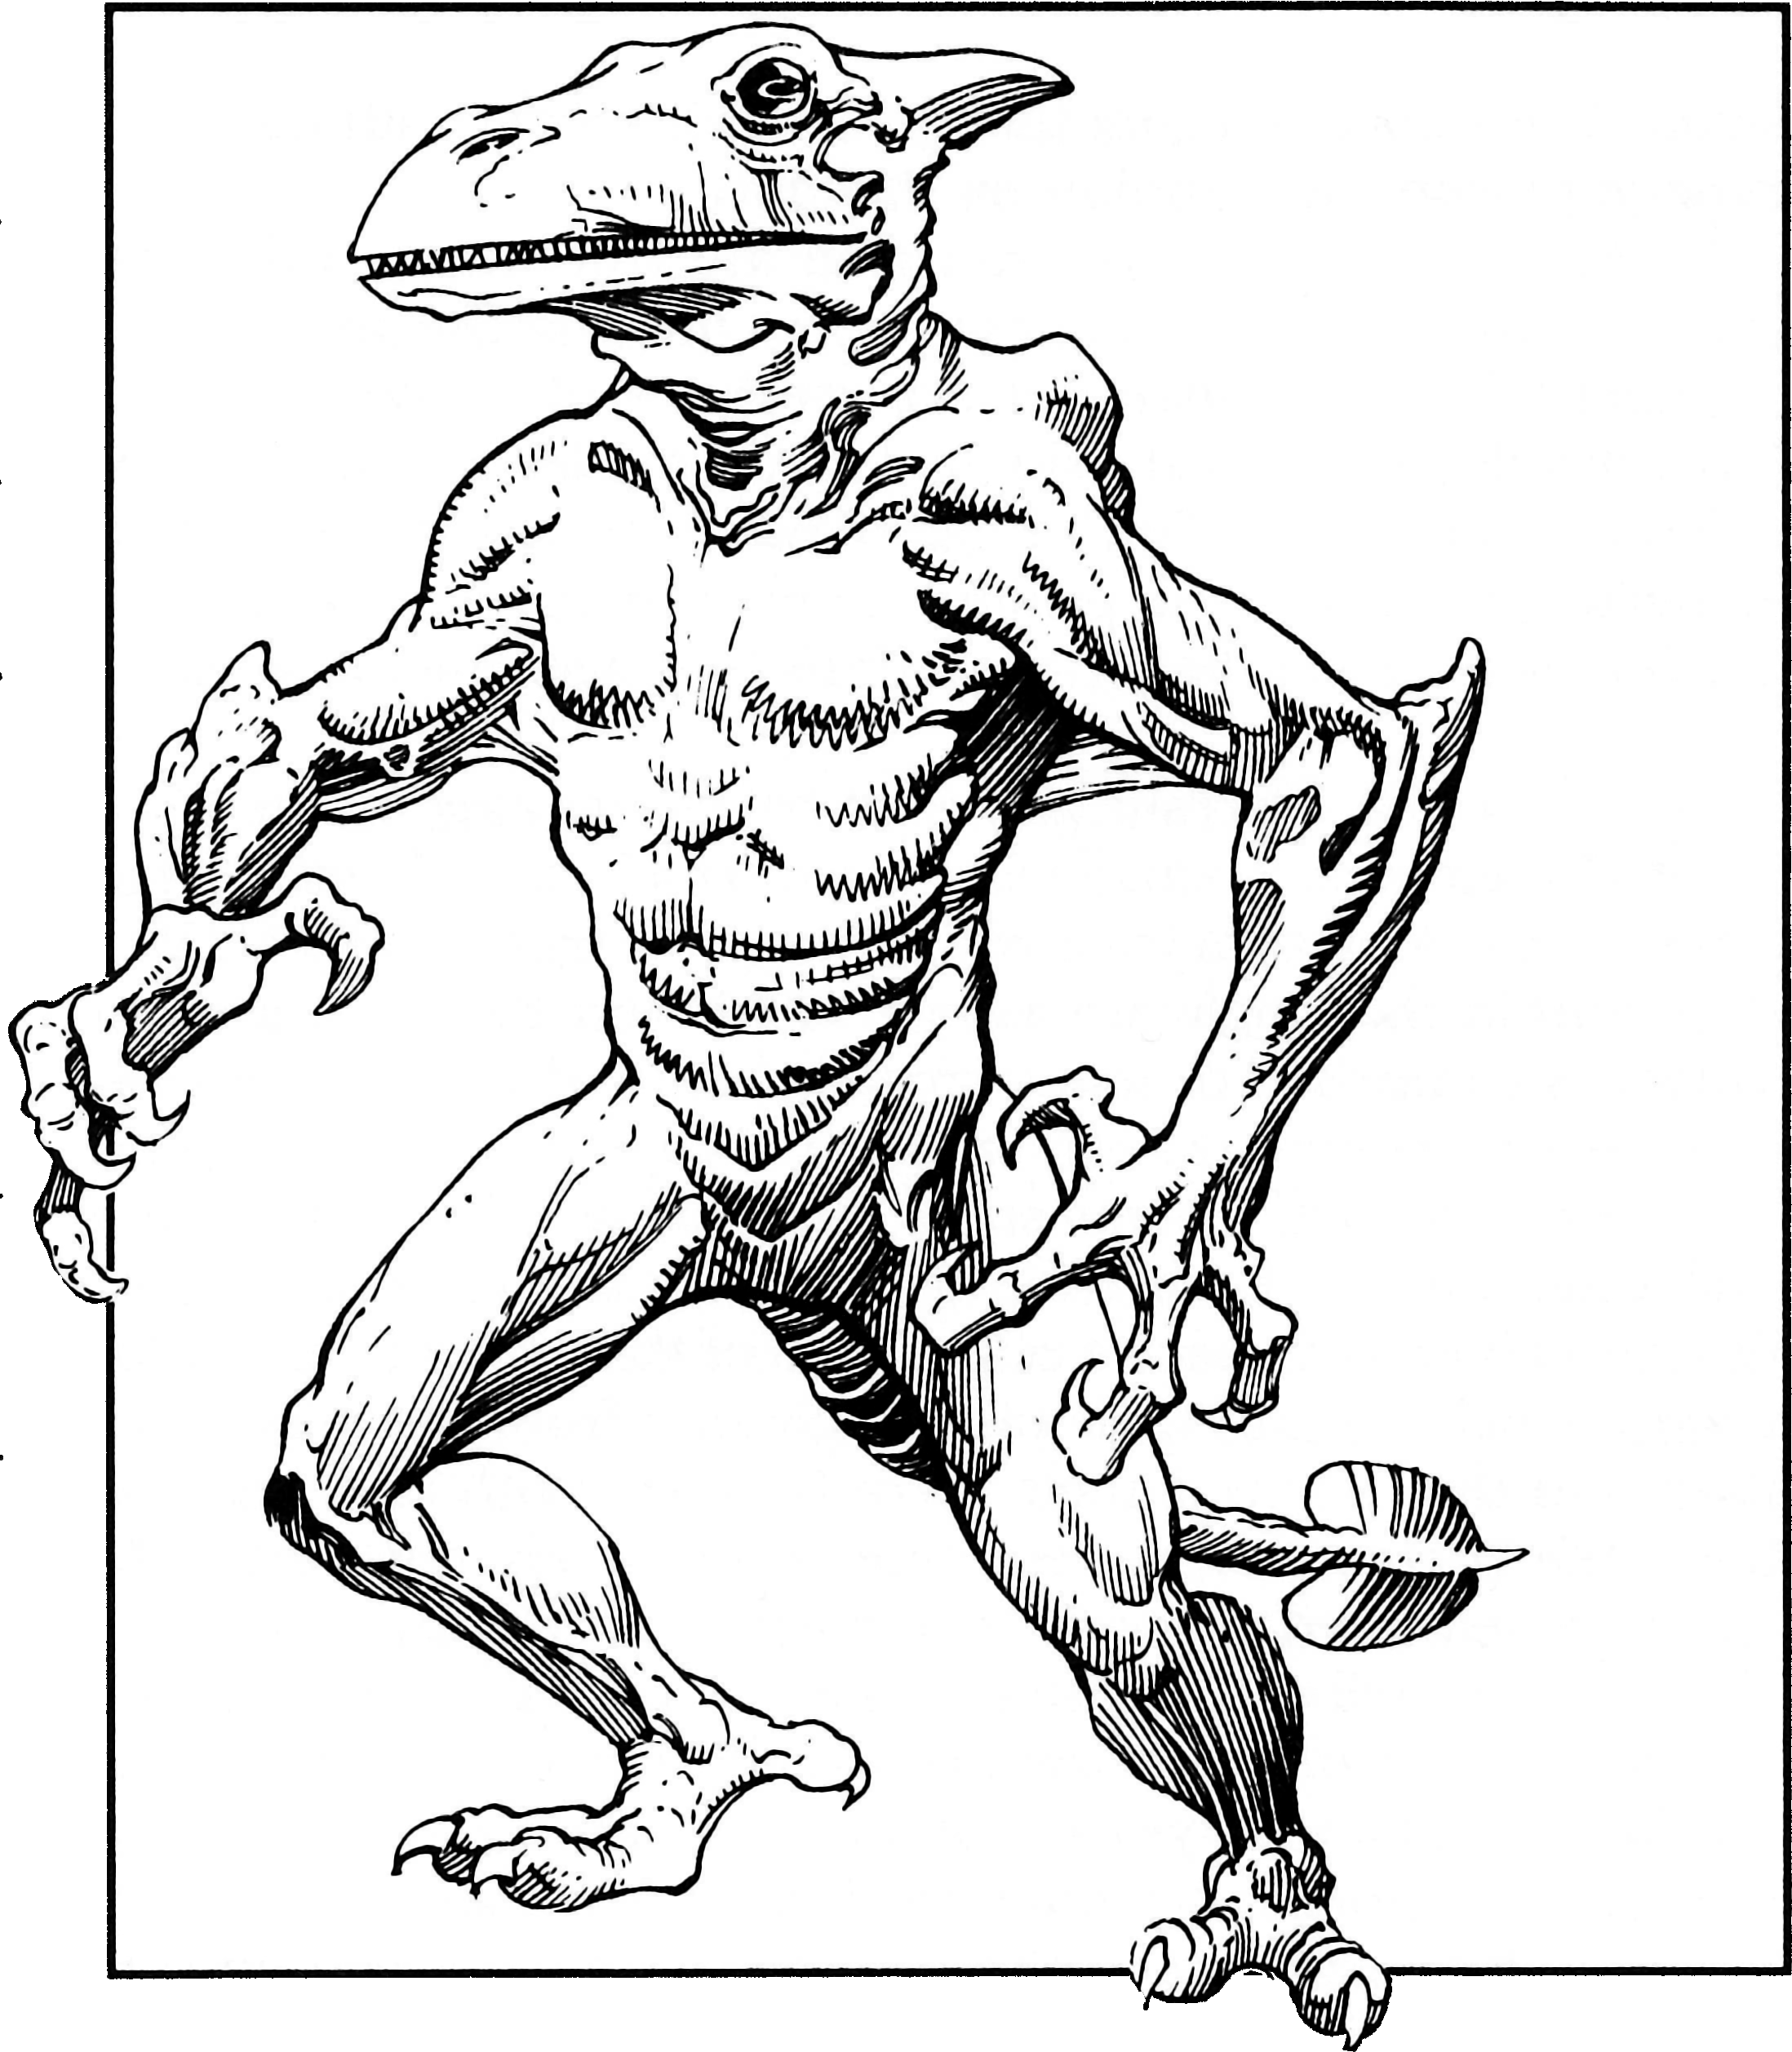
\includegraphics[width=\columnwidth]{images/pterran-1.png}
\end{figure}

Pterrans are rarely seen in the Tablelands. They live their lives in the Hinterlands, rarely leaving the safety of their villages. However, the recent earthquake and subsequent storms have brought disruption into the pterran's lives. More pterrans now venture outside their homes, and come to the Tyr region to seek trade and information.

\textbf{Personality:} Among strangers, pterrans seem like subdued, cautious beings, but once others earn a pterran's trust, they will find an individual that is open, friendly, inquisitive, and optimistic. In other respects, a pterran's personality is largely shaped by her chosen life path: Pterrans who choose the path of the warrior are less disturbed by the brutality of the Tablelands; they are constantly examining their surroundings and considering how the terrain where they are standing could be defended; they take greatest satisfaction from executing a combat strategy that results in victory without friendly casualties. Pterrans who choose the path of the druid are most interested in plants, animals, and the state of the land; they take greatest satisfaction when they eliminate a threat to nature. Pterrans that choose the path of the mind are most interested in befriending and understanding other individuals and societies; these telepaths take greatest satisfaction from intellectual accomplishments such as solving mysteries, exposing deception, resolving quarrels between individuals, and establishing trade routes between communities.

\textbf{Physical Description:} Pterrans are 1.5 to 1.9 meters tall reptiles with light brown scaly skin, sharp teeth, and a short tail. Pterrans wear little clothing, preferring belts and loincloths, or sashes. They walk upright, like humanoids, and have opposing thumbs and three-fingered, talon-clawed hands. Pterrans have two shoulder stumps, remnants of wings they possessed long ago, and a finlike growth juts out at the back of their heads. Pterrans weigh between 90 to 110 kilograms. There is no visible distinction between male and female pterrans.

\textbf{Relations:} Pterrans are new to the Tablelands, and unaccustomed to cultures and practices of the region. They have learned to not judge too quickly. Their faith in the Earth Mother means they undertake their adventure with open minds, but they will remain subdued and guarded around people they do not trust. A pterran's respect for the Earth Mother governs all his behavior. Creatures that openly destroy the land or show disrespect for the creatures of the wastes are regarded suspiciously. Pterrans understand the natural cycle of life and death, but have difficulty with some aspects of the city life, such as cramped living spaces, piled refuse, and the smells of unwashed humanoids.

\textbf{Alignment:} Pterrans tend towards lawful, well-structured lives, and most of them are good. Evil pterran adventurers are usually outcasts who have committed some horrible offense.

\textbf{Pterran Lands:} Most adventuring pterrans come from one of two villages in the Hinterlands, southwest of the Tyr regions: Pterran Vale and Lost Scale.

\textbf{Magic:} The wizard's use of the environment as a source of power conflicts with a pterran's religious beliefs. Pterrans will cautiously tolerate members of other races who practice preserving magic, if the difference is explained to them.

\textbf{Psionics:} Virtually all pterrans have a telepathic talent, and pterran psions are nearly universally telepaths. Telepathy is considered one of the honored pterran ``life paths.''

\textbf{Religion:} Pterrans worship the Earth Mother, a representation of the whole world of Athas. Their devotion to the Earth Mother is deeply rooted in all aspects of their culture, and it defines a pterran's behavior. All rituals and religious events are related to their worship of the Earth Mother. Religious events include festivals honoring hunts or protection from storms, with a priest presiding over the celebration. Most pterran priests are druids.

\textbf{Language:} Pterran speak Saurian with an accent that is difficult for other races to understand. The long appendage at the back of their head enables them to create sounds that no other race in the Tablelands can reproduce. The sounds are low, and resonate through the pterran's crest. Humanoid vocal chords cannot reproduce such sounds. Pterrans learn the Common tongue easily, but speak it with a slight, odd accent.

\textbf{Names:} Pterrans earn their first name just after they hatch, based on the weather and season of their hatching. After the pterran has decided upon a Life Path and has completed their apprenticeship, she receives title that becomes the first part of her name. This marks her transition into pterran society. There are a number of traditional names associated with each Life Path, but names do not always come from these ranks.

\textbf{Male Names:} Airson, Darksun, Earthsong, Suntail, Goldeye, Onesight, Terrorclaw.

\textbf{Female Names:} Cloudrider, Greenscale, Lifehearth, Rainkeeper, Spiritally, Watertender.

\textbf{Path Name:} Aandu, Caril, Dsar, Everin, Illik, Myril, Odten, Qwes, Pex, Ptellac, Ristu, Ssrui, Tilla, Xandu.

\textbf{Tribe or Village Names:} Pterran Vale, Lost Scale

\textbf{Adventurers:} Pterrans adventure because they believe the recent earthquake and disturbing events are signs from the Earth Mother that they should get more involved in the planet's affairs. They believe that these recent upheavals of nature are signs that the Earth Mother needs help, and this is a call the pterrans will gladly accept. As such, the most brave and adventurous of the pterrans have begun to establish contact with Tyr and some merchant houses, hoping to expand their contacts and information.

\subsection{Pterran Society}
Pterran society is based largely on ceremony and celebrations. An area is set aside in the center of each village for ceremonies. Pterrans revere the world of Athas as the Earth Mother, and believe themselves to be her favored children. Throughout the day, they engage in a number of ceremonies that give thanks to the Earth Mother. These are led by druids who play a very important role in pterran society.

A pterran village is a collection of many smaller family dwellings. Pterrans always bear young in pairs.

At age 15 every pterran chooses a ``life path.'' The three main life paths are the path of the warrior, the path of the druid and the path of the psionicist, though lesser life paths exist as well.

More pterrans follow the path of the warrior than any of the other paths, and become protectors of their villages as well as the tribe's weapon makers.

Pterrans that choose the path of the druid provide an important role in the daily ceremonies to the Earth Mother.

Fewer pterrans choose the path of the psionicist than the other two major paths, as psionics are viewed as outside of nature. Psionicists are viewed with suspicion by the rest of the tribe; however, they do provide valuable skills to the tribe and are often the tribe's negotiators when they meet outsiders.

Pterrans are omnivores. Much of their diet comes from hunting animals and raising crops. Kirre, id fiend, and flailer are all considered pterran delicacies.

\subsection{Roleplaying Suggestions}
Remember your character class is your ``life path.'' You think of yourself, and present yourself first and foremost as a druid, a warrior or a psion. Remember your daily celebrations and giving of thanks to the Earth Mother. You can usually find a reason to be grateful. Disrespect for the land angers you, since the whole land has withered under the disrespect of foolish humans and others. You celebrate with song and with dance. You have a good sense of humor but it does not extend to blasphemies such as defiling. In initial role-playing situations, you are unfamiliar with the customs and practices of the societies of the Tyr Region. However, you are not primitive by any definition of the word. You look upon differences with curiosity and a willingness to learn, as long as the custom doesn't harm the Earth Mother or her works.

\subsection{Pterran Racial Traits}
\begin{itemize*}
    \item $-2$ Dexterity, +2 Wisdom, +2 Charisma: Pterrans' strong confidence and keen instincts for others' motives make them keen diplomats, and when they take the path of the psion, powerful telepaths.
    \item Humanoid (psionic, reptilian): Pterrans are humanoid creatures with the psionic and reptilian subtypes.
    \item Medium: As Medium creatures, pterrans have no special bonuses or penalties due to size.
    \item Pterran base land speed is 9 meters.
    \item Poor Hearing: Pterrans have only slits for ears, and their hearing sense is diminished. Pterrans suffer a $-2$ penalty to Listen checks.
    \item Natural Weaponry: Pterrans can use their natural weapons instead of fighting with crafted weapons if they so choose. A pterran can rake with their primary claw attack for 1d3 of damage for each claw, and they bite for 1d4 points of damage as a secondary attack.
    \item Psi-Like Ability: At will---\psionic{missive}. All pterrans are gifted from the day they hatch with the ability to communicate telepathically, but only with their fellow reptiles. Manifester level is equal to \onehalf Hit Dice (minimum 1st).
    \item Weapon Familiarity: The following weapon is treated as martial rather than as an exotic weapon: thanak. This weapon is more common among pterrans than among other races.
    \item Automatic Languages: Saurian. Bonus Languages: Common, Dwarven, Elven, Halfling, Giant, Gith, Kreen, and Yuan-ti. Pterran know the languages of the few intelligent creatures that live in the Hinterlands.
    \item Life Path: A pterran's life path determines his favored class. Those following the Path of the Druid have druid as a favored class; the Path of the Mind gives psion as a favored class, while the Path of the Warrior gives ranger as a favored class. A Pterran chooses a life path upon coming of age, and the path cannot be changed once chosen at character creation time.
\end{itemize*}
\section{Thri-kreen}
\Quote{This one does not speak with the quivering soft shells that lay about all night. This one might eat you, but never speak.}{Tu'tochuk}

\Figure*{t}{images/thrikreen-1.png}

Thri-kreen are the strangest of the intelligent races of the Tablelands. These insectoid beings possess a mindset very different from any humanoid being encountered. They roam the wastes in packs, hunting for food day and night, since they require no sleep. Thri-kreen are quick and agile and make fearsome fighters, feared throughout the wastes.

\textbf{Personality:} Since thri-kreen (also known simply as the kreen) do not require sleep, they have difficulty understanding this need in the humanoid races. They have difficulty understanding this state of ``laziness'' in others. Other behaviors of humanoids seem unnecessarily complex. A keen's life is simple: hunt prey. Kreen live for the hunt, and own only what they can carry.

\textbf{Physical Description:} Mature thri-kreen stand about 2.1 meters tall, with a rough body length of 3.3 meters. Their four arms end in claws; their two legs are extremely powerful, capable of incredible leaps. However, kreen are unable to jump backwards. Their body is covered with a sandy-yellow chitin, a tough exoskeleton that grants the thri-kreen protection from blows. Their head is topped with two antennae, and their two eyes are compound and multifaceted. The kreen mouth consists of small pincers. Male and female thri-kreen are physically indistinguishable. Thri-kreen usually do not wear clothing, but wear some sort of harness to carry weapons and food. Many wear leg or armbands, or bracelets. Some attach rings on different places on their chitin, though this requires careful work by a skilled artisan.

\textbf{Relations:} The pack mentality dominates a keen's relation with others. Kreen hunt in packs, small groups that assemble together. Kreen will hunt prey in the same region for a while, but move on before their prey has been depleted. A kreen that joins a group of humanoids will often try to establish dominance in the group. This can be disconcerting to those unaware of the keen's behavior, since establishing dominance usually means making threatening gestures. Once the matter is settled, they will abide by the outcome. Thri-kreen view humanoids as sources of food, though they don't usually hunt them, only in dire need. Many kreen have a particularly fond taste for elves; as such, meetings between these two races are often tense. However, once part of a clutch, thri-kreen will never turn on their humanoid friends, even in the worst of situations.

\textbf{Alignment:} Most thri-kreen are lawful, since the pack mentality is ingrained in their beings. Kreen that deviate from this mentality are rare.

\textbf{Kreen Lands:} No thri-kreen settlements exist in the Tyr region; kreen encountered there are either small packs of kreen, or else adventuring with humanoids. To the north of the Tyr region, beyond the Jagged Cliffs, past the Misty Border, lies the Kreen Empire. This great nation of kreen rules the Crimson Savanna, forming great city-states that rival the humanoid city-states of the Tyr region.

\textbf{Magic:} Thri-kreen have no natural disposition towards magic, and a wizard's use of the environment as a source of power conflicts with a keen's beliefs. As well, the keen's lack of sleep and its instinctual need to hunt do not lend themselves well to magical study. Kreen wizards are extremely rare: no one has ever seen one in the Tablelands.

\textbf{Psionics:} Kreen view psionics as a natural part of their existence. Some packs rely on telepathy to communicate with each member and coordinate their hunting abilities. Many kreen also use psionic powers to augment their already formidable combat prowess. Psychometabolic powers are often used to boost speed, metabolism or strength to gain an advantage in combat. Most kreen (even non-adventurers) take the psychic warrior class, which kreen consider a natural part of growing up. Kreen do not need instruction to advance in the psychic warrior class---it comes to them as part of their ancestral memory.

\textbf{Religion:} Thri-kreen have no devotion to any god, but they hold nature and the elements in high regard. Ancestral memories guide them through their lives. Thri-kreen revere the Great One, a legendary kreen leader from the past.

\textbf{Language:} The Kreen language is very different from those of the other intelligent races. They have no lips or tongues, and so cannot make the same sounds humanoids make. Kreen language is made up of clicks, pops, or grinding noises.

\textbf{Names:} Kachka, Ka'Cha, Ka'Ka'Kyl, Klik-Chaka'da, Sa'Relka, T'Chai

\textbf{Adventurers:} Kreen adventure for different reasons. Most enjoy challenges presented by new prey. Some seek out the challenge of leading new clutches, new companions and observing the different ``hunting'' techniques of the dra (sentient meat-creatures such as humans).

\subsection{Thri-Kreen Society}
Thri-kreen hatch from eggs. All those who hatch at the same time form what is called a clutch. Thri-kreen gather in packs that roam the wastes. Each pack consists of several clutches that roam over an area that the pack considers theirs to hunt on. There are no permanent thri-kreen communities.

Clutches and packs are organized along strict order of dominance. The toughest member is leader; the second most powerful is second in command and so forth. A thri-kreen can challenge a superior for dominance initiating a contest. The contestants fight until one surrenders or dies. Afterwards, the matter is considered settled and there are no lingering resentments between victor and loser. The pack-mates take the view that the challenger was only acting to strength the pack.

Thri-kreen are obsessed with hunting. They are carnivores, but seldom hunt intelligent life for food. They do have a taste for elf, which gives them a bad reputation amongst Elven tribes. When not hunting, they craft weapons, teach their young, and craft sculptures.

The pack mentality is so ingrained in the culture that thri-kreen apply it to every situation. Thri-kreen feel compelled to be part of a clutch and will accept members of other races as clutch-mates.

\subsection{Roleplaying Suggestions}
You tend to rely on your natural attacks and special kreen weapons. Everything you kill is a potential dinner. You have a strong need for a party leader---obedience to this leader in the party is important to you. If you seem to be the most powerful and capable, then you will assume leadership; if someone challenges your authority then you will wish to test whether they are in fact stronger than you. It is not a question of vanity; you won't want to fight to the death, but merely to ascertain who is worthy to lead the party. You do not have the focus of a dwarf to complete a project, but you would give your life to protect your companions. If you did not trust and honor them as your own family, then you would not travel with them and work together with them. You do not understand the concept of sleep. It disturbs you that your dra companions lie unconscious for a third of their lifetimes. You own only what you can carry, caring little for money or other items that other races consider as treasure. Your philosophy of ownership sometimes leads you into conflict with presumptuous dra who think they can own buildings, land, and even whole herds of cattle!


% \Figure*{t}{images/adventurer-2.png}


\subsection{Thri-Kreen Racial Traits}
\begin{itemize*}
    \item +4 Dexterity, $-2$ Intelligence, +2 Wisdom, $-4$ Charisma: Thri-kreen are fast, but their alien mindset makes it difficult for them to relate to humanoids; furthermore, their ``clutch-mind'' instincts leave them with a poor sense of themselves as individuals.
    \item Monstrous Humanoid: Thri-kreen are not subject to spells or effects that affect humanoids only, such as \spell{charm person} or \spell{dominate person}.
    \item Medium: Thri-kreen receive no advantages or penalties due to size.
    \item Thri-kreen base land speed is 12 meters.
    \item Low-light Vision: Thri-kreen can see twice as far as a human in moonlight and similar conditions of poor illumination, retaining the ability to distinguish color and detail.
    \item Vestigial Antennae: Thri-kreen lessen miss chance from any type of concealment by 5\% (including total concealment or blindness). Thri-kreen have 15\% miss chance against foes with concealment, and 45\% miss chance against enemies with total concealment or when the thri-kreen is blinded.
    \item Sleep Immunity: Thri-kreen do not sleep, and are immune to sleep spells and similar effects. Thri-kreen spellcasters and manifesters still require 8 hours of rest before preparing spells or regaining power points.
    \item Water Efficient: Thri-kreen can go for one week on the amount of water a human needs in a day.
    \item Natural Armor: Thri-kreen have a +2 natural armor bonus to AC due to their naturally tough and resistant chitin.
    \item Multiple Limbs: Thri-kreen have four arms, and thus can take the \feat{Multiweapon Fighting} feat instead of the \feat{Two-Weapon Fighting} feat. Thri-kreen can also take the \feat{Multiattack} feat. (These are not bonus feats.)
    \item Natural Weapons: Thri-kreen may make bite and claw attacks as a full round action. Their primary claw attack does 1d4 points of damage for each of their four claws. Their secondary bite attack, deals 1d4 points of damage, and has a chance to poison. A thri-kreen can attack with a weapon (or multiple weapons) at its normal attack bonus, and make either a bite or claw attack as a secondary attack.
    \item Deflect Arrows: Thri-kreen gain the benefit of the \feat{Deflect Arrows} feat.
    \item Leap (Ex): When a thri-kreen reaches 3 Hit Dice, they become natural jumpers, gaining a +30 racial bonus to all \skill{Jump} checks.
    \item Poison (Ex): When a thri-kreen reaches 5 Hit Dice, their glands become able to deliver poison with a successful bite attack. Fortitude DC 11 + Con modifier. The initial and secondary damages are paralysis for 1d10 rounds.
    \item Weapon Familiarity: To thri-kreen, the chatkcha and gythka are treated as martial rather than exotic weapons. These weapons are more common among thri-kreen than among other races.
    \item Thri kreen have a +4 racial bonus on \skill{Hide} checks in sandy or arid areas.
    \item Alien Mind (Ex): A thri-kreen has difficulty understanding how the humanoid minds work. Whenever a thri-kreen targets a creature of another race with mind-affecting abilities, that creature gains +1 to its save against those powers.
    \item Automatic Languages: Kreen. Bonus Languages: Common, Dwarven, Elven, Entomic, Saurian, and Terran.
    \item Favored Class: Druid or Fighter. A thri-kreen must choose between druid or fighter as favored class. This choice cannot be changed. A multiclass thri-kreen's chosen class does not count when determining whether he takes an experience point for multiclassing.
    \item Level Adjustment: +1.
\end{itemize*}


\section{Other Races}
Athas is a place where members of different races are usually found in the same city-state, usually because they are going to be used in gladiatorial games as an exotic attraction, or to become slaves due to their physical might. Even though they are not usually concentrated on a specific area, these races are significant players in the Tablelands. It is only fitting then, that belgoi, gith, jozhals, ssurrans, tareks, taris, yuan-tis, and a variety of other creatures commonly viewed as monsters might appear as player characters in a {\tableheader Dark Sun} campaign. Cultural information about several monstrous races appears in \hyperref[chapter:Life on Athar]{Life on Athas}.

\Chapter{Character Classes}
{From the lowliest slave to the highest templar, our fates are decided for us. The slave at the hands of the master, and the templar at the will of the king. Pray to Ral and Guthay that your children are born when the stars align to favor them. Few are those privileged to choose their own path of life, and cursed are those for they are bound by choice and have but themselves to blame for their misfortune. The bard addicted to his alchemical mixtures, the templar imprisoned for his crimes, and the gladiator sacrificed for the thrill of the fight. It is the choices that define who you are and how you die, regardless of who makes them.}{The Oracle, Blue Shrine Scrolls}
\section{The Classes}

\Capitalize{Y}{ou} may notice that there are some classes not described here. Some of these are core classes that have been deemed inappropriate to the feel of the {\tableheader Dark Sun} campaign setting. Others are classes from previous editions of {\tableheader Dark Sun} that don't fit in the 3e.

\textbf{Monk:} There are several monasteries on Athas, though little evidence in previous material supports the martial artist variety of monk. Monks are too few in number to warrant a core class.

\textbf{Paladin:} The idea of doing good for its own sake runs contrary to the tone and theme of the setting. There are no gods to reward selfless acts, and no grand traditions of chivalry and nobility to promote. In essence, Athas is a world where evil behavior is the norm.

\textbf{Sorcerer:} Mechanically, a sorcerer's spontaneous casting and a psion's manifesting are similar, thus including the sorcerer removes some of the uniqueness of the psion. Some also feel that an arcane spellcaster without a spellbook violates the flavor of the setting.

\textbf{Soulknife:} There is no precedent of a concept such as the soulknife in any previous material. However, in a metal-poor, high psionic world, the ability to manifest a weapon using the mind has its place. There would probably not be enough soulknives to warrant a core class, which would need to be shoehorned into the existing campaign world.

\textbf{Trader:} The trader class, present in previous editions of the setting is not included here because it's benefits and traits are nearly all encompassed in the standard set of 3rd edition skills. Reproducing the class is easily done using a standard skill-focused class, like the rogue or bard, or using the expert NPC class.

Some DMs choose to run {\tableheader Dark Sun} as a low-magic, low treasure campaign. In such games, the monk and soulknife could become unbalanced because of their lack of dependence on treasure.

DMs are free to include any of the above core classes in their games, but these classes will not appear in any official releases.

\subsection{The Power Point Reserve}
Psionic characters fuel their abilities through a pool, or reserve, of power points. Your power point reserve is equal to your base power points gained from your class, bonus power points from a high key ability score (see Abilities and Manifesters, below), and any additional bonus power points from sources such as your character race and feat selections.

\subsubsection{Multiclass Psionic Characters}
If you have levels in more than one psionic class, you combine your power points from each class to make up your reserve. You can use these power points to manifest powers from any psionic class you have.

While you maintain a single reserve of power points from your class, race, and feat selections, you are still limited by the manifester level you have achieved with each power you know.

\Class{Barbarian}
{Gith's blood! I will hunt that wizard down and skin him alive.}{Borac, mul barbarian}

Brutality is a way of life in Athas, as much in some of the cities as in the dwindling tribes of Athas' harsh wastes. Cannibal headhunting halflings (who occasionally visit Urik from the Forest Ridge) sometimes express shock at the savagery and bloodshed of the folk that call themselves ``civilized'' and live between walls of stone. They would be more horrified if they were to see the skull piles of Draj, experience the Red Moon Hunt in Gulg, or watch a seemingly docile house slave in Eldaarich rage as she finally ``goes feral'', taking every frustration of her short cruel life out on whoever happens to be closest to hand. Nibenese sages claim that the potential for savagery is in every sentient race, and the history of Athas seems to support their claim.

Some on Athas have turned their brutality into an art of war. They are known as ``brutes'', ``barbarians'' or ``feral warriors'' and they wear the name with pride. Impious but superstitious, cunning and merciless, fearless and persistent, they have carved a name for their martial traditions out of fear and blood.

\WarriorTable{The Barbarian}{
1 & +1 & +2 & +0 & +0 & Fast movement, rage 1/day \\
2 & +2 & +3 & +0 & +0 & Uncanny dodge \\
3 & +3 & +3 & +1 & +1 & Wasteland trap sense +1 \\
4 & +4 & +4 & +1 & +1 & Rage 2/day \\
5 & +5 & +4 & +1 & +1 & Improved uncanny dodge \\
6 & +6/+1 & +5 & +2 & +2 & Wasteland trap sense +2 \\
7 & +7/+2 & +5 & +2 & +2 & Damage reduction 1/-- \\
8 & +8/+3 & +6 & +2 & +2 & Rage 3/day \\
9 & +9/+4 & +6 & +3 & +3 & Wasteland trap sense +3 \\
10 & +10/+5 & +7 & +3 & +3 & Damage reduction 2/-- \\
11 & +11/+6/+1 & +7 & +3 & +3 & Greater rage \\
12 & +12/+7/+2 & +8 & +4 & +4 & Rage 4/day, wasteland trap sense +4 \\
13 & +13/+8/+3 & +8 & +4 & +4 & Damage reduction 3/-- \\
14 & +14/+9/+4 & +9 & +4 & +4 & Indomitable will \\
15 & +15/+10/+5 & +9 & +5 & +5 & Wasteland trap sense +5 \\
16 & +16/+11/+6/+1 & +10 & +5 & +5 & Damage reduction 4/--, rage 5/day \\
17 & +17/+12/+7/+2 & +10 & +5 & +5 & Tireless rage \\
18 & +18/+13/+8/+3 & +11 & +6 & +6 & Wasteland trap sense +6 \\
19 & +19/+14/+9/+4 & +11 & +6 & +6 & Damage reduction 5/-- \\
20 & +20/+15/+10/+5 & +12 & +6 & +6 & Mighty rage, rage 6/day}

\subsection{Making a Barbarian}

The barbarian is a fearsome warrior, compensating for lack of training and discipline with bouts of powerful rage. While in this berserk fury, barbarians become stronger and tougher, better able to defeat their foes and withstand attacks. These rages leave barbarians winded; at first they only have the energy for a few such spectacular displays per day, but those few rages are usually sufficient.

\textbf{Races:} Humans are often barbarians, many having been raised in the wastes or escaped from slavery. Half-elves sometimes become barbarians, having been abandoned by their elven parents to the desert to survive on their own; if more of them survived they would be quite numerous. Dwarves are very rarely barbarians, but their mul half-children take to brutishness like a bird takes to flight, living by their wits and strengths in the wastes. Muls have a particular inclination this way of life, and very often ``go feral'' in the wilderness after escaping slavery in the city. Elves rarely take to the barbarian class; those that do are usually from raiding tribes such as the Silt Stalkers. Half-giants readily take the barbarian class. Despite their feral reputations, halflings rarely become barbarians; their small statures and weak strength adapts them better for the ranger class. Likewise, despite their wild nature, thri-kreen are rarely barbarians, since their innate memories allow them to gain more specialized classes such as ranger and psychic warrior without training. Pterrans of the Forest Ridge occasionally become barbarians, but like halflings they more often favor the ranger class.

\textbf{Alignment:} Barbarians are never lawful---their characteristic rage is anything but disciplined and controlled. Many barbarians in the cities are often rejects from the regular army, unable to bear regular discipline or training. Some may be honorable, but at heart they are wild. At best, chaotic barbarians are free and expressive. At worst, they are thoughtlessly destructive.

\subsection{Game Rule Information}
\textbf{Alignment:} Any nonlawful.

\textbf{Hit Die:} d12.

\subsubsection{Class Skills}
\skill{Climb} (Str), \skill{Craft} (Int), \skill{Escape Artist} (Des), \skill{Handle Animal} (Cha), \skill{Intimidate} (Cha), \skill{Jump} (Str), \skill{Listen} (Wis), \skill{Profession} (Wis), \skill{Ride} (Dex), and \skill{Survival} (Wis).

\textbf{Skill Points per Level:} 4 + Int modifier ($\times4$ at 1st level).

\subsubsection{Class Features}

\textbf{Weapon and Armor Proficiency:} A barbarian is proficient with all simple and martial weapons, light armor, medium armor, and shields (except tower shields).

\textbf{Fast Movement (Ex):} A barbarian's land speed is faster than the norm for his race by +10 feet. This benefit applies only when he is wearing no armor, light armor, or medium armor and not carrying a heavy load. Apply this bonus before modifying the barbarian's speed because of any load carried or armor worn.

\textbf{Rage (Ex):} A barbarian can fly into a rage a certain number of times per day. In a rage, a barbarian temporarily gains a +4 bonus to Strength, a +4 bonus to Constitution, and a +2 morale bonus on Will saves, but he takes a $-2$ penalty to Armor Class. The increase in Constitution increases the barbarian's hit points by 2 points per level, but these hit points go away at the end of the rage when his Constitution  score drops back to normal. (These extra hit points are not lost first the way temporary hit points are.) While raging, a barbarian cannot use any Charisma-, Dexterity-, or Intelligence-based skills (except for \skill{Balance}, \skill{Escape Artist}, \skill{Intimidate}, and \skill{Ride}), the \skill{Concentration} skill, or any abilities that require patience or concentration, nor can he cast spells or activate magic items that require a command word, a spell trigger (such as a wand), or spell completion (such as a scroll) to function. He can use any feat he has except \feat{Combat Expertise}, item creation feats, and metamagic feats. A fit of rage lasts for a number of rounds equal to 3 + the character's (newly improved) Constitution modifier. A barbarian may prematurely end his rage. At the end of the rage, the barbarian loses the rage modifiers and restrictions and becomes fatigued ($-2$ penalty to Strength, $-2$ penalty to Dexterity, can't charge or run) for the duration of the current encounter (unless he is a 17th-level barbarian, at which point this limitation no longer applies).

A barbarian can fly into a rage only once per encounter. At 1st level he can use his rage ability once per day. At 4th level and every four levels thereafter, he can use it one additional time per day (to a maximum of six times per day at 20th level). Entering a rage takes no time itself, but a barbarian can do it only during his action, not in response to someone else's action. 

\textbf{Uncanny Dodge (Ex):} At 2nd level, a barbarian retains his Dexterity bonus to AC (if any) even if he is caught flat-footed or struck by an invisible attacker. However, he still loses his Dexterity bonus to AC if immobilized. If a barbarian already has uncanny dodge from a different class, he automatically gains improved uncanny dodge instead.

\textbf{Wasteland Trap Sense (Ex):} Starting at 3rd level, a barbarian gains a +1 bonus on Reflex saves made to avoid traps and natural hazards, and a +1 dodge bonus to AC against attacks made by traps and natural hazards. These bonuses rise by +1 every three barbarian levels thereafter (6th, 9th, 12th, 15th, and 18th level). Trap sense bonuses gained from multiple classes stack.

\textbf{Improved Uncanny Dodge (Ex):} At 5th level and higher, a barbarian can no longer be flanked. This defense denies a rogue the ability to sneak attack the barbarian by flanking him, unless the attacker has at least four more rogue levels than the target has barbarian levels. If a character already has uncanny dodge from a second class, the character automatically gains improved uncanny dodge instead, and the levels from the classes that grant uncanny dodge stack to determine the minimum level a rogue must be to flank the character.

\textbf{Damage Reduction (Ex):} At 7th level, a barbarian gains Damage Reduction. Subtract 1 from the damage the barbarian takes each time he is dealt damage from a weapon or a natural attack. At 10th level, and every three barbarian levels thereafter (13th, 16th, and 19th level), this damage reduction rises by 1 point. Damage reduction can reduce damage to 0 but not below 0.

\textbf{Greater Rage (Ex):} At 11th level, a barbarian's bonuses to Strength and Constitution during his rage each increase to +6, and his morale bonus on Will saves increases to +3. The penalty to AC remains at $-2$.

\textbf{Indomitable Will (Ex):} While in a rage, a barbarian of 14th level or higher gains a +4 bonus on Will saves to resist enchantment spells. This bonus stacks with all other modifiers, including the morale bonus on Will saves he also receives during his rage.

\textbf{Tireless Rage (Ex):} At 17th level and higher, a barbarian no longer becomes fatigued at the end of his rage.

\textbf{Mighty Rage (Ex):} At 20th level, a barbarian's bonuses to Strength and Constitution during his rage each increase to +8, and his morale bonus on Will saves increases to +4. The penalty to AC remains at $-2$.

\subsubsection{Ex-Barbarians}

A barbarian who becomes lawful loses the ability to rage and cannot gain more levels as a barbarian. He retains all the other benefits of the class (damage reduction, fast movement, wasteland trap sense, and uncanny dodge).

\subsection{Playing a Barbarian}

All cower and stand in awe at the fury you can tap, enhancing your strength and toughness. But what do these people know of the burnt wastes of Athas, the hellish jungles of the Forest Ridge? The cruel vicissitudes of growing up in the wastes of Athas were nothing but normal to you. When your family was lost in a tembo attack, or when your entire village was either murdered or forced into slavery, how could you not know they might not had to die? These and many other brutal experiences marked you, and you now stand apart from those born into the ``comforts'' of the city-states.

\subsubsection{Religion}

Although most are profoundly superstitious, barbarians distrust the established elemental temples of the cities. Some worship the elements of fire or air or devote themselves to a famous figure. Most barbarians truly believe the sorcerer-kings to be gods, because of their undeniable power, and a few actually worship a sorcerer-king, usually the one that conquered their tribe. Such barbarians often escape menial slavery by joining an elite unit of barbarians in the service of an aggressive city-state such as Urik, Draj or Gulg.

\subsubsection{Other Classes}

Barbarians are most comfortable in the company of gladiators, and of clerics of Air and Fire. Enthusiastic lovers of music and dance, barbarians admire bardic talent, and some barbarians also express fascination with bardic poisons, antidotes and alchemical concoctions. With some justification, barbarians do not trust wizardry. Even though many barbarians manifest a wild talent, they tend to be wary of psions and Tarandan psionicists. Psychic warriors, on the other hand, are creatures after the barbarian's own heart, loving battle for its own sake. Barbarians have no special attitudes toward fighters or rogues. Barbarians admire gladiators and will ask about their tattoos and exploits, but will quickly grow bored if the gladiator does not respond boastfully.

\subsubsection{Combat}

You know that half the battle occurs before the fight even begins. You prefer to choose your battleground when you can, stalking your opponent into terrain that best suits your abilities. Once battle is joined, you become a wild frenzy of motion, striking quickly and powerfully until all your opponents are crushed. While you lack the training of the fighter, or the cunning of the gladiator, you more than compensate them through sheer power and resilience.

\subsubsection{Advancement}

Becoming a barbarian let you further tap into your feral nature, letting you become one with the savage beast in your hear, and through your training, you have learned what you must do to unlock it.

To fully utilize your barbarian abilities, you will want to focus on feats that take advantage of your superior strength and speed, such as Power Attack and Whirlwind Attack.

\subsection{Starting Packages}
\subsubsection{The Survivor}
Human Barbarian

\textbf{Ability Scores:} Str 15, Dex 13, Con 14, Int 10, Wis 12, Cha 8.

\textbf{Skills:} \skill{Climb}, \skill{Escape Artist}, \skill{Listen}, \skill{Survival}.

\textbf{Languages:} Common.

\textbf{Feat:} \feat{Great Fortitude}, \feat{Wastelander}.

\textbf{Weapons:} Carrikal (1d8/x3)

Atlatl with 10 javelins (1d6/x3, 40 ft.).

\textbf{Armor:} Scale mail (+4 AC).

\textbf{Gear:} Standard adventurer's kit, 13 Cp.

\subsubsection{The Crusher}
Half-giant Barbarian

\textbf{Ability Scores:} Str 23, Dex 10, Con 18, Int 6, Wis 9, Cha 4.

\textbf{Skills:} \skill{Climb}, \skill{Intimidate}, \skill{Jump}.

\textbf{Languages:} Common.

\textbf{Feat:} \feat{Exotic Weapon Proficiency} (swatter).

\textbf{Weapons:} Swatter (3d8/x4).

\textbf{Armor:} Leather (+2 AC).

\textbf{Gear:} Standard adventurer's kit, 0 Cp.

\subsubsection{The Hunter}
Thri-kreen Barbarian

\textbf{Ability Scores:} Str 15, Dex 14, Con 12, Int 10, Wis 13, Cha 8.

\textbf{Skills:} \skill{Jump}, \skill{Knowledge} (nature), \skill{Search}, \skill{Survival}.

\textbf{Languages:} Kreen.

\textbf{Feat:} \feat{Track}.

\textbf{Weapons:} Four chatkchas (1d6, 20 ft.).

\textbf{Armor:} Heavy wooden shield (+2 AC).

\textbf{Gear:} Standard adventurer's kit, 13 Cp.

\subsection{Barbarians on Athas}
\Quote{Don't make my friend angry. You won't like him when he's angry.}{Cabal, half-elven bard}

In a savage world like Athas, is only natural that some of its inhabitants have turned into barbarians. They are fierce combatants without the army training fighters receive or wild rangers without the hunting skills.

\subsubsection{Daily Life}

A barbarian is a passionate adventurer. As a survivalist, he often sees his involvement in a particular enterprise as a validation of his superior strength and resilience. In his mind, his presence alone is enough to ensure the success of a quest, adventure, or ruin raid. Even simple tasks are additional opportunities to prove his own worth by accomplishing the task with might and alacrity. Barbarians are typically hardheaded and unforgiving because of the rigors of his previous life.

\subsubsection{Notables}

It is rare for a barbarian to live long enough, or close enough to civilization, in order to become famous, but a few examples exist. Korno, a Raamite gladiator, became the leader of a group of slaves, and Korno's furious rage known from the arenas has only increased after losing everything in the Raam invasion by Dregoth. The leader of Pillage, Chilod, is a tarek know for his outbursts of rage and cruelty, being one of the most feared chiefs of the Bandit States.

\subsubsection{Organizations}

Because of their independent and sometimes downright chaotic natures, many barbarians refuse to join organizations of any kind, though they usually maintain relationships with trading houses and raiding tribes. There is no specific organization that binds barbarians together.

\subsubsection{NPC Reactions}

Many lay people cannot tell a barbarian from a ranger or a fighter until his rage overcomes him and he starts screaming and bashing. Most authority figures and templars do not appreciate barbarians since they are prone to losing control and cannot be truly trusted. Thus, they generally treat barbarians with a great deal of caution.

\subsubsection{Barbarian Lore}

Characters with ranks in \skill{Knowledge} (nature) can research barbarians to learn more about them. When a character makes a skill check, read or paraphrase the following, including the information from lower DCs.

\textbf{DC 10:} Barbarians are hot-blooded combatants who fight with great brutality and savagery.

\textbf{DC 15:} Barbarians become stronger and more resilient when they lose control.

\textbf{DC 20:} Barbarians can stand up to punishment that no other individual can endure, and their reflexes are as quick as a rogue's.
\section{Bard}
\Quote{Some people think a club can solve any problem. Unless you're a half-giant, there are more sophisticated ways of settling a disagreement.}{Cabal, half‐elven bard}

From the shadowy corners of Athas' most disreputable places hails the bard. Like their counterparts in other fantasy worlds, Athasian bards are the unquestioned masters of oral tradition and forgotten lore, but rather than sharing their lore with whoever will listen, Athasian bards guard their secrets as jealously as the sorcerer‐kings harbor their water and iron. Athasian bards may sell information to the highest bidder; they peddle their services and the fruits of their knowledge, but trade secrets are what give bards an edge on the uninitiated. Bards would rather die than reveal these secrets.

Meeting a bard can be an uneasy encounter, since one never knows how the bard has chosen to devote his multiple talents. Some bards master the art of making poisons, and survive by selling these poisons and their antidotes for those who have coin to pay. Some bards master the art of entertainment, using their performances to amuse nobles and templars and gain wealth. Some become assassins, mixing their knowledge of poison and stealth to become hired hands. Bards' unique position in the Athasian society means they often overhear conversations between high‐ranking templars or nobles, or they may have treated an injured person that prefers to remain anonymous. Respectable folk despise them; the powerful fear them; but in the Athasian cities, everyone eventually comes to need their services.

\WarriorTable[b{0.8cm} b{2.6cm} Z{1.4cm} Z{1.4cm} Z{1.4cm} X]{The Bard}{
1 & +0 & +2 & +2 & +2 & Bardic music, bardic knowledge, smuggler, countersong, fascinate, inspire courage +1\\
2 & +1 & +3 & +3 & +3 & Poison use, streetsmart\\
3 & +2 & +3 & +3 & +3 & Inspire competence, quick draw\\
4 & +3 & +4 & +4 & +4 & Trade secret\\
5 & +3 & +4 & +4 & +4 & Mental resistance\\
6 & +4 & +5 & +5 & +5 & Improved poison use, suggestion, quick thinking +2\\
7 & +5 & +5 & +5 & +5 & Chance 1/day\\
8 & +6/+1 & +6 & +6 & +6 & Inspire courage +2, trade secret\\
9 & +6/+1 & +6 & +6 & +6 & Inspire greatness, speed reactions\\
10 & +7/+2 & +7 & +7 & +7 & Slippery mind\\
11 & +8/+3 & +7 & +7 & +7 & Quick thinking +4\\
12 & +9/+4 & +8 & +8 & +8 & Song of freedom, trade secret\\
13 & +9/+4 & +8 & +8 & +8 &  \\
14 & +10/+5 & +9 & +9 & +9 & Chance 2/day, inspire courage +3\\
15 & +11/+6/+1 & +9 & +9 & +9 & Defensive roll, inspire heroics\\
16 & +12/+7/+2 & +10 & +10 & +10 & Quick thinking +6, trade secret\\
17 & +12/+7/+2 & +10 & +10 & +10 & Awareness \\
18 & +13/+8/+3 & +11 & +11 & +11 & Mass suggestion, mindblank\\
19 & +14/+9/+4 & +11 & +11 & +11 &  \\
20 & +15/+10/+5 & +12 & +12 & +12 & Inspire courage +4, trade secret}
\subsection{Making a Bard}

Bards receive numerous abilities they can use to survive. Many become masters of poisons, selling their illegal substances to anyone. Alone of the classes, bards hold the secrets of alchemy, creating fiery concoctions and mysterious mixes. Bards are master smugglers, selling spell components and other illegal items in the Bard's Quarters of the city‐states. All bards, however, have some degree of entertainment skill. The songs of most bards can dazzle a crowd, or incite them to riot. Bards tend to learn to play a variety of instruments, or recite poetry or old legends by campfire. They can be acrobats, performing dazzling displays of physical prowess. They are often called upon as sources of information.

\textbf{Abilities:} Charisma is the most important ability for a bard, because many of their abilities and skills are affected by it. A high Dexterity improves the bard's defensive ability. Intelligence is also important because it bolster the numbers of skills he has access.

\textbf{Races:} All humanoid races of Athas can become bards. The social stigma in certain regions may be higher than others, however. For example, the loremasters of the halflings of the Jagged Cliffs are highly regarded because of the ancient secrets and histories they preserve. But in the city‐states, where the Bard's Quarters are notorious, being a bard is not usually a good thing. Elven tribes often have a bard, who keeps the history of the tribe alive, its conquests and defeats. Humans are often bards, becoming performers of great talent, or assassins of deadly skill and precision. Half‐elves, because of their lonely existence, often take to being bards. The prejudice they face at every stage in life can move some to become great poets or singers. Muls and half‐giants make poor bards; their talents are usually better served elsewhere than the stage or the shadows of alleys. As well, thri‐kreen are rarely seen as bards, relying instead upon their racial memory.

\textbf{Alignment:} Most bards are chaotic, and operate alone, brokering information, arranging deals, smuggling illegal wares such as poisons, drugs, spell components and other things. Neutral bards are the ones most likely to operate in fellowships with adventurers, or entertain in troupes with other bards. The rare lawful bards can easily secure positions as councilors or agents for templars, and noble and merchant houses. Good bards are often entertainers or lorekeepers, putting their talents to benevolent use, sometimes diagnosing poisonings and selling the proper antidotes. Evil bards are often masters of poisons and alchemy, selling their wares to anyone with the ceramic to pay.

\subsection{Game Rule Information}

\textbf{Hit Die:} d6.

\subsection{Class Skills}

\textbf{Class Skills:} Appraise (Int), Balance (Dex), Bluff (Cha), Climb (Str), Craft (Int), Decipher Script (Int), Diplomacy (Cha), Disguise (Cha), Escape Artist (Dex), Forgery (Int), Gather Information (Cha), Heal (Wis), Hide (Dex), Intimidate (Cha), Jump (Str), Knowledge (all skills individually) (Int), Listen (Wis), Move Silently (Dex), Perform (Cha), Profession (Wis), Ride (Dex), Search (Int), Sense Motive (Wis), Sleight of Hand (Dex), Speak Language (n/a), Tumble (Dex), Use Magic Device (Cha), Use Psionic Device (Cha), Use Rope (Dex).

\textbf{Skill Points per Level:} 6 + Int modifier (x4 at 1st level).

\subsection{Class Features}

\textbf{Weapon and Armor Proficiency:} You are proficient in all simple weapons, plus the bard's friend, all crossbows, garrote, greater blowgun, whip and widow's knife. You are proficient in light armor, but not shields.

Bardic Knowledge: A bard may make a special bardic knowledge check with a bonus equal to his bard level + his Intelligence modifier to see whether he knows some relevant information about local notable people, legendary items, or noteworthy places. (If the bard has 5 or more ranks in Knowledge (history), he gains a +2 bonus on this check.)
A successful bardic knowledge check will not reveal the powers of a magic item but may give a hint as to its general function. A bard may not take 10 or take 20 on this check; this sort of knowledge is essentially random.

\Table{}{p{0.6cm} X}{
\tableheader DC & \tableheader Type of Knowledge\\
10 & Common, known by at least a substantial minority of the local population.\\
20 & Uncommon but available, known by only a few people legends.\\
25 & Obscure, known by few, hard to come by.\\
30 & Extremely obscure, known by very few, possibly forgotten by most who once knew it, possibly known only by those who don't understand the significance of the knowledge.}

\textbf{Bardic Music:} Once per day per bard level, a bard can use his song or poetics to produce magical effects on those around him (usually including himself, if desired). While these abilities fall under the category of bardic music and the descriptions discuss singing or playing instruments, they can all be activated by reciting poetry, chanting, singing lyrical songs, singing melodies, whistling, playing an instrument, or playing an instrument in combination with some spoken performance. Each ability requires both a minimum bard level and a minimum number of ranks in the Perform skill to qualify; if a bard does not have the required number of ranks in at least one Perform skill, he does not gain the bardic music ability until he acquires the needed ranks.

Starting a bardic music effect is a standard action. Some bardic music abilities require concentration, which means the bard must take a standard action each round to maintain the ability. Even while using bardic music that doesn't require concentration, a bard cannot cast spells, activate magic items by spell completion (such as scrolls), spell trigger (such as wands), or command word. Just as for casting a spell with a verbal component, a deaf bard has a 20\% chance to fail when attempting to use bardic music. If he fails, the attempt still counts against his daily limit.

\textit{Countersong (Su):} A bard with 3 or more ranks in a Perform skill can use his music or poetics to counter magical effects that depend on sound (but not spells that simply have verbal components). Each round of the countersong, he makes a Perform check. Any creature within 30 feet of the bard (including the bard himself) that is affected by a sonic or language-dependent magical attack may use the bard's Perform check result in place of its saving throw if, after the saving throw is rolled, the Perform check result proves to be higher. If a creature within range of the countersong is already under the effect of a noninstantaneous sonic or language-dependent magical attack, it gains another saving throw against the effect each round it hears the countersong, but it must use the bard's Perform check result for the save. Countersong has no effect against effects that don't allow saves. The bard may keep up the countersong for 10 rounds.

\textit{Fascinate (Sp):} A bard with 3 or more ranks in a Perform skill can use his music or poetics to cause one or more creatures to become fascinated with him. Each creature to be fascinated must be within 90 feet, able to see and hear the bard, and able to pay attention to him. The bard must also be able to see the creature. The distraction of a nearby combat or other dangers prevents the ability from working. For every three levels a bard attains beyond 1st, he can target one additional creature with a single use of this ability.

To use the ability, a bard makes a Perform check. His check result is the DC for each affected creature's Will save against the effect. If a creature's saving throw succeeds, the bard cannot attempt to fascinate that creature again for 24 hours. If its saving throw fails, the creature sits quietly and listens to the song, taking no other actions, for as long as the bard continues to play and concentrate (up to a maximum of 1 round per bard level). While fascinated, a target takes a $-4$ penalty on skill checks made as reactions, such as Listen and Spot checks. Any potential threat requires the bard to make another Perform check and allows the creature a new saving throw against a DC equal to the new Perform check result.

Any obvious threat, such as someone drawing a weapon, casting a spell, or aiming a ranged weapon at the target, automatically breaks the effect. Fascinate is an enchantment (compulsion), mind-affecting ability.

\textit{Inspire Courage (Su):} A bard with 3 or more ranks in a Perform skill can use song or poetics to inspire courage in his allies (including himself), bolstering them against fear and improving their combat abilities. To be affected, an ally must be able to hear the bard sing. The effect lasts for as long as the ally hears the bard sing and for 5 rounds thereafter. An affected ally receives a +1 morale bonus on saving throws against charm and fear effects and a +1 morale bonus on attack and weapon damage rolls. At 8th level, and every six bard levels thereafter, this bonus increases by 1 (+2 at 8th, +3 at 14th, and +4 at 20th). Inspire courage is a mind-affecting ability.

\textit{Inspire Competence (Su):} A bard of 3rd level or higher with 6 or more ranks in a Perform skill can use his music or poetics to help an ally succeed at a task. The ally must be within 30 feet and able to see and hear the bard. The bard must also be able to see the ally.

The ally gets a +2 competence bonus on skill checks with a particular skill as long as he or she continues to hear the bard's music. Certain uses of this ability are infeasible. The effect lasts as long as the bard concentrates, up to a maximum of 2 minutes. A bard can't inspire competence in himself. Inspire competence is a mind-affecting ability.

\textit{Suggestion (Sp):} A bard of 6th level or higher with 9 or more ranks in a Perform skill can make a suggestion (as the spell) to a creature that he has already fascinated. Using this ability does not break the bard's concentration on the fascinate effect, nor does it allow a second saving throw against the fascinate effect.

Making a suggestion doesn't count against a bard's daily limit on bardic music performances. A Will saving throw (DC 10 + \unichar{"00BD} bard's level + bard's Cha modifier) negates the effect. This ability affects only a single creature (but see mass suggestion, below). Suggestion is an enchantment (compulsion), mind-affecting, language dependent ability.

\textit{Inspire Greatness (Su):} A bard of 9th level or higher with 12 or more ranks in a Perform skill can use music or poetics to inspire greatness in himself or a single willing ally within 30 feet, granting him or her extra fighting capability. For every three levels a bard attains beyond 9th, he can target one additional ally with a single use of this ability (two at 12th level, three at 15th, four at 18th). To inspire greatness, a bard must sing and an ally must hear him sing. The effect lasts for as long as the ally hears the bard sing and for 5 rounds thereafter. A creature inspired with greatness gains 2 bonus Hit Dice (d10s), the commensurate number of temporary hit points (apply the target's Constitution modifier, if any, to these bonus Hit Dice), a +2 competence bonus on attack rolls, and a +1 competence bonus on Fortitude saves. The bonus Hit Dice count as regular Hit Dice for determining the effect of spells that are Hit Dice dependent. Inspire greatness is a mind-affecting ability.

\textit{Song of Freedom (Sp):} A bard of 12th level or higher with 15 or more ranks in a Perform skill can use music or poetics to create an effect equivalent to the break enchantment spell (caster level equals the character's bard level). Using this ability requires 1 minute of uninterrupted concentration and music, and it functions on a single target within 30 feet. A bard can't use song of freedom on himself.

\textit{Inspire Heroics (Su):} A bard of 15th level or higher with 18 or more ranks in a Perform skill can use music or poetics to inspire tremendous heroism in himself or a single willing ally within 30 feet. For every three bard levels the character attains beyond 15th, he can inspire heroics in one additional creature. To inspire heroics, a bard must sing and an ally must hear the bard sing for a full round. A creature so inspired gains a +4 morale bonus on saving throws and a +4 dodge bonus to AC. The effect lasts for as long as the ally hears the bard sing and for up to 5 rounds thereafter. Inspire heroics is a mind-affecting ability.

\textit{Mass Suggestion (Sp):} This ability functions like suggestion, above, except that a bard of 18th level or higher with 21 or more ranks in a Perform skill can make the suggestion simultaneously to any number of creatures that he has already fascinated. Mass suggestion is an enchantment (compulsion), mind-affecting, language-dependent ability.

\textbf{Smuggler (Ex):} A bard receives a +1 insight bonus to Bluff and Sleight of Hand checks for every two bard levels.

\textbf{Poison Use:} Bards are trained in the use of poisons, and as of 2nd level, never risk accidentally poisoning themselves when applying poison to a blade.

\textbf{Streetsmart (Ex):} When a bard reaches 2nd level, he gets a +2 competence bonus to Gather Information and Intimidate checks.

\textbf{Quick Draw:} Bards learn to strike quickly and without warning. At 3rd level, a bard gains Quick Draw as a bonus feat.

\textbf{Trade Secrets:} At every 4th level a bard learns a trade secret chosen from the list below.

\textit{Alchemy Dealer:} A bard with this trade secret pays one‐half of the market price for raw materials needed to craft alchemical items.

\textit{Accurate:} When a bard with this trade secret attacks an armored opponent, his accuracy allows him to ignore 1 point of natural armor bonus to AC or 1 point of armor bonus to AC. This trade secret may be chosen more than once, and its effects stack.

\textit{Agile:} A bard with this trade secret receives a +1 dodge bonus to AC. This trade secret may be chosen more than once, and its effects stack.

\textit{Coolheaded:} A bard with this trade secret may take 10 on Bluff and Diplomacy checks.

\textit{Improvised Materials:} A bard with this trade secret can craft poisons from raw materials at hand instead of relying on specific ingredients. Doing so increases the Craft (poisonmaking) check DC by 5 but otherwise has no effect on the poison's potency.

\textit{Poison Dealer:} A bard with this trade secret pays one‐half of the market price for raw materials needed to craft poisons.

\textit{Poisonbane:} A bard with this trade secret receives a +4 insight bonus to Craft (alchemy) checks when creating antitoxin and poison antidotes.

\textit{Poison Resistance:} A bard with this trade secret receives a +4 bonus to saving throws against poisons.

\textit{Scorpion's Touch:} A bard with this trade secret adds +1 to the save DC of all poisons applied by him. This trade secret may be chosen more than once, and its effects stack.

\textit{Skilled:} A bard with this trade secret adds one‐half your bard level (rounded down) as a competence bonus to one of the following skills: Appraise, Bluff, Craft, Diplomacy, Heal, Perform, Profession, Sense Motive or Sleight of Hand. This trade secret may be chosen more than once, each time it applies to a different skill.

\textit{Smokestick Application:} A bard with this trade secret can combine inhaled poisons with smokesticks. All creatures within the area the smokestick covers (10‐ft. cube) are affected by the poison you applied to the smokestick.

\textit{Versatile:} A bard with this trade secret selects any two non‐class skills to be considered class skills.

\textbf{Mental Resistance (Ex):} Bards carry many dark secrets they would prefer remain secret. This, combined with a large amount of knowledge based on half‐truths and false rumors makes your mind unreliable to those who would seek to mentally affect it. A 5th level bard receives a +2 morale bonus to saves made against telepathic powers and enchantment/charm spells.

\textbf{Improved Poison Use (Ex):} At 6th level, a bard can apply poison to a weapon as a free action without provoking attacks of opportunity.

\textbf{Quick Thinking (Ex):} Bards often find themselves in a tight spot where they have to act quickly, whether it is to escape a templar patrol or strike first when in confrontation with a foe. At 6th level, a bard gets a +2 bonus on initiative checks. This bonus increases by 2 at 11th and 16th level.

\textbf{Chance (Ex):} Bards live on the edge in many ways. At 7th level, a bard may reroll one single d20 roll once per day, but have to keep the latter result--for better or for worse. At 14th level, a bard may use this ability two times per day.

\textbf{Speed Reactions (Ex):} Beginning at 9th level, when a bard uses the attack action or full attack action in melee, he may subtract a number from all melee attack rolls and add the same number to his initiative. This number may not exceed his base attack bonus. He may not make ranged attacks this round. The initiative increase takes effect on the next round. The new initiative is his initiative for the remainder of the combat, unless you were to use speed reactions again, which would increase your initiative further.

\textbf{Slippery Mind (Ex):} If a 10th level bard is affected by an enchantment spell or effect and fails her saving throw, she can attempt it again 1 round later at the same DC. She gets only this one extra chance to succeed on her saving throw.

\textbf{Defensive Roll (Ex):} At 15th level a bard learns how to avoid a potentially lethal blow to take less damage from it than you otherwise would. Once per day, when he would be reduced to 0 or fewer hit points by damage in combat (from a weapon or other blow, not a spell or special ability), the bard can attempt to roll with the damage. To use this ability, the bard must attempt a Reflex saving throw (DC = damage dealt). If the save succeeds, he takes only half damage from the blow; if it fails, he takes full damage. He must be aware of the attack and able to react to it in order to execute his defensive roll — if he is denied her Dexterity bonus to AC, he can't use this ability. Since this effect would not normally allow a character to make a Reflex save for half damage, the rogue's evasion ability does not apply to the defensive roll.

\textbf{Awareness (Ex):} At 17th level, you are never caught flat‐footed and always act in the surprise round.

\textbf{Mind Blank (Sp):} At 18th level your mind becomes completely sealed against involuntary intrusion as per the mindblank spell. This spell‐like ability is always considered active.

\subsection{Playing a Bard}

You are a master of oral tradition and lore, and a true artist, but you share your talents only with those who can afford to pay you.

You are an artist. You are the center of attention (whenever you want to), the person everyone wants to talk to, the “face” of the party. Even if you aren't the most attractive or charismatic member of your group, your unequaled skill at performance arts creates an irresistible appeal born of justified confidence. You are more than just light entertainment, though. Your target rarely survives the encounter if you don't want him to.

You might adventure because you desire entertainment. Someone with your smarts gets bored easily. Alternatively, you may have been blacklisted on your current location because of a “business transaction” gone wrong. You have to keep moving, and adventuring offers you a regular change of scenery. In any case, a life of adventure allows you to see new things, meet interesting people, and get some silvers in the process.

\subsection{Religion}

No central bardic organization exists, and more often than not bards have no particular penchant for religion. Some may worship the elements, fearing the power of the elemental forces, and most bards tend to relate to the Air ever‐changing nature, but bards that worship sorcerer‐kings are rare. A lifestyle of breaking the rules of the city‐states does not lend one to worship the lawgivers.

\subsection{Other Classes}

Bards face life as it comes, and usually hold no special grudge or awe for any one class. They usually approach other's profession on the basis of how it can help them at the moment. Clerics and druids are respected for their devotion to a divine force, but usually not held in awe. Fighters, gladiators and rangers can be useful as sword-arms but are otherwise useless to the bard. Bards do not view wizards with the same aversion as others might view them, since bards sell them their components.

\subsection{Combat}

A bard rarely seeks to initiate combat -- instead he skulks about, looking for an opportunity to strike swiftly, using his poisons to their greatest advantage. Your work best with teammates, maneuvering to get flanks and help bring down opponents with your various poisons. Use your bardic music to bolster your allies and distract your opponents while the real heavy hitters in your group mop them up.

\subsection{Advancement}

You have a flexibility in building your talents unrivaled by any other class. You can either emphasize on ability or nurse a broad range of abilities. In most cases, feats that consistently improve your talents are more useful than feats that function in only certain situations.

As you advance in the class, continue to max out your ranks in Bluff and Perform, and invest skill points in Gather Information and Sleight of Hand. Many feats in the Athasian Emporium supplement make the most of your poison abilities. Improved Feint is an excellent choice with your expertise in Bluff, and Greasing the Wheels (page 72) if perfect for getting around templar inspections. If you play up the assassin aspect of this class, consider magic (or psionic) items that help you cloak your true intentions, such as an amulet of proof against detection and location or a veil of lies (page 260).

When multiclassing or taking a level in a prestige class, find combinations that further broaden your abilities or that increase your flexibility. The poisonmaster prestige class (page 101), the dune trader (page 90), and the assassin (DMG 180) deserve special mention. They are a great combination with the bard class.

\subsection{Starting Packages}
\subsubsection{The Assassin}

Elf Bard

\textbf{Ability Scores:} Str 13, Dex 17, Con 10, Int 10, Wis 14, Cha 8.

\textbf{Skills:} Climb, Disguise, Hide, Move Silently, Open Lock, Spot.

\textbf{Languages:} Elven, Common.

\textbf{Feat:} Stealthy.

\textbf{Weapons:} Bard's friend (1d4/18-20)

Shortbow with 20 arrows (1d6/x3, 60 ft.).

\textbf{Armor:} Studded leather (+3 AC).

\textbf{Gear:} Standard adventurer's kit, thieves' tools, musical instrument, 9 Cp.

\subsubsection{The Information Smuggler}

Human Bard

\textbf{Ability Scores:} Str 8, Dex, 12, Con 10, Int 15, Wis 14, Cha 13.

\textbf{Skills:} Bluff, Decipher Script, Diplomacy, Gather Information, Knowledge (local), Listen, Sense Motive.

\textbf{Languages:} City language, Common, Elven.

\textbf{Feat:} Investigator, Negotiator.

\textbf{Weapons:} Widow's knife (1d4/x3)

Light crossbow with 20 bolts (1d8/19-20, 80 ft.).

\textbf{Armor:} Leather armor (+2 AC).

\textbf{Gear:} Standard adventurer's kit, 4 Cp.

\subsubsection{The Poisoner}

Half‐elf Bard

\textbf{Ability Scores:} Str 8, Dex 15, Con 10, Int 15, Wis 14, Cha 6.

\textbf{Skills:} Appraise, Craft (alchemy), Craft (poisonmaking), Knowledge (local), Sleight of Hand.

\textbf{Languages:} City language, Common, Elven.

\textbf{Feat:} Skill Focus (Craft [poisonmaking]).

\textbf{Weapons:} Bard's friend (1d4/18-20)

Blowgun with 20 needles (1, 10 ft.).

\textbf{Armor:} Shell armor (+4 AC).

\textbf{Gear:} Standard adventurer's kit, smokestick, 4 Cp.
\vskip10em
\subsection{Bards on Athas}
\Quote{She was a rare beauty: charming, graceful, talented. It's too bad she killed my boss.}{Talos, mul bodyguard}

Athasian bards use songs and tales as their tools of trade. A bard is a person of wit and camaraderie. Despite having few other talents to offer, the bard is a welcome source of entertainment and information across Athas. However, bards are noted to be extremely untrustworthy and even ruthless -- they often sell their skills as assassins and poison alchemists to the highest bidder.

In the cities, bards often become tools of the nobility. They're commonly hired by one noble house and sent to another as a gift. The bards are sent not only to entertain, but usually to perform some other subtle task as well (such as robbery, espionage, or even assassination).

Nobles consider it rude to turn down the gift of a bard or bard company. However, when presented with a troop of bards from one's worst enemy, it's sometimes better to be rude and turn them away, for the consequences of their visit could be downright deadly. To get around this, the noble who hired them sometimes disguises their approach by having another noble send them. A very complicated collage of intrigue and deceit is often woven wherever bards are involved.

\subsubsection{Daily Life}

The way a bard behaves depends on his individual sense of morality. Some think nothing of adopting false identities, smuggling forbidden goods, or even coldblooded assassination. Other bards find themselves driven to use their skills to entertain and help people.

Bards can become great leaders. With their quick wits and great charisma, bards would be natural leaders were it not for their inconstancy. If a bard manages to earn the trust of companions, they value his leadership. Lacking that trust, a bard rarely leads for long.

\subsubsection{Notables}

Bards often gain notoriety for their deeds, although most prefer to remain behind false identities. The human bard only known as Wheelock has become a legend when it comes to creating poisons. Fyrian Wynder is a Tyrian half‐elven bard notorious for his combination of bardic abilities and the Way, since his acting skills enable him to adopt several identities, while his psionic abilities provide a means of gaining access to secured areas and going unnoticed once he gets there.

\subsubsection{Organizations}

Bards don't organize together, but they often linger around the same places, which end up getting known as the Bard's Quarter in most city‐states. A bard joining an organization probably has a specific goal (or target) in mind and rakes a position that best allows him to attain it. A long‐term commitment to such a group rarely appeals to a bard.

\subsubsection{NPC Reactions}

Common folk ten to have a hard time differentiating bards from rogues. Bards further confuse the issue by regularly adopting false identities and hiding their varied abilities. Thus, the reaction a bard gets from those he meets depends on what he is pretending to be at a time. Individuals who know about the bard class and the reputation that comes with it have an initial attitude one step more hostile than normal. Templars in particular look poorly upon bards, since they know of the various illegal activities they usually perform.

\subsubsection{Bard Lore}

Characters with ranks in Knowledge (local) can research bards to learn more about them. When a character makes a skill check, read or paraphrase the following, including the information from lower DCs.

\textbf{DC 15:} Bards are jacks of all trades, masters of performance and deception, and information smugglers.

\textbf{DC 20:} Bards are masters of poisons and lore, and they have many of the skills of rogues.
\vskip10em
\section{Cleric}
\Quote{Without destruction, there is nothing to build.}{Credo of the fire cleric}

In a world without gods, spiritualism on Athas has unlocked the secrets of the raw forces of which the very planet is comprised: earth, air, fire, and water. However, other forces exist which seek to supplant them and rise to ascendancy in their place. These forces have taken up battle against the elements of creation on the element's own ground in the form of entropic perversions of the elements themselves: magma, rain, silt and sun.

\SpellcasterTable{The Cleric}{.5cm}{
1 & +0 & +2 & +0 & +2 & Turn or rebuke undead & 3 & 1+1 &  &  &  &  &  &  &  &  \\
2 & +1 & +3 & +0 & +3 &  & 4 & 2+1 &  &  &  &  &  &  &  &  \\
3 & +2 & +3 & +1 & +3 &  & 4 & 2+1 & 1+1 &  &  &  &  &  &  &  \\
4 & +3 & +4 & +1 & +4 &  & 5 & 3+1 & 2+1 &  &  &  &  &  &  &  \\
5 & +3 & +4 & +1 & +4 &  & 5 & 3+1 & 2+1 & 1+1 &  &  &  &  &  &  \\
6 & +4 & +5 & +2 & +5 &  & 5 & 3+1 & 3+1 & 2+1 &  &  &  &  &  &  \\
7 & +5 & +5 & +2 & +5 &  & 6 & 4+1 & 3+1 & 2+1 & 1+1 &  &  &  &  &  \\
8 & +6/+1 & +6 & +2 & +6 &  & 6 & 4+1 & 3+1 & 3+1 & 2+1 &  &  &  &  &  \\
9 & +6/+1 & +6 & +3 & +6 &  & 6 & 4+1 & 4+1 & 3+1 & 2+1 & 1+1 &  &  &  &  \\
10 & +7/+2 & +7 & +3 & +7 &  & 6 & 4+1 & 4+1 & 3+1 & 3+1 & 2+1 &  &  &  &  \\
11 & +8/+3 & +7 & +3 & +7 &  & 6 & 5+1 & 4+1 & 4+1 & 3+1 & 2+1 & 1+1 &  &  &  \\
12 & +9/+4 & +8 & +4 & +8 &  & 6 & 5+1 & 4+1 & 4+1 & 3+1 & 3+1 & 2+1 &  &  &  \\
13 & +9/+4 & +8 & +4 & +8 &  & 6 & 5+1 & 5+1 & 4+1 & 4+1 & 3+1 & 2+1 & 1+1 &  &  \\
14 & +10/+5 & +9 & +4 & +9 &  & 6 & 5+1 & 5+1 & 4+1 & 4+1 & 3+1 & 3+1 & 2+1 &  &  \\
15 & +11/+6/+1 & +9 & +5 & +9 &  & 6 & 5+1 & 5+1 & 5+1 & 4+1 & 4+1 & 3+1 & 2+1 & 1+1 &  \\
16 & +12/+7/+2 & +10 & +5 & +10 &  & 6 & 5+1 & 5+1 & 5+1 & 4+1 & 4+1 & 3+1 & 3+1 & 2+1 &  \\
17 & +12/+7/+2 & +10 & +5 & +10 &  & 6 & 5+1 & 5+1 & 5+1 & 5+1 & 4+1 & 4+1 & 3+1 & 2+1 & 1+1 \\
18 & +13/+8/+3 & +11 & +6 & +11 &  & 6 & 5+1 & 5+1 & 5+1 & 5+1 & 4+1 & 4+1 & 3+1 & 3+1 & 2+1 \\
19 & +14/+9/+4 & +11 & +6 & +11 &  & 6 & 5+1 & 5+1 & 5+1 & 5+1 & 5+1 & 4+1 & 4+1 & 3+1 & 2+1 \\
20 & +15/+10/+5 & +12 & +6 & +12 &  & 6 & 5+1 & 5+1 & 5+1 & 5+1 & 5+1 & 4+1 & 4+1 & 3+1 & 3+1}


\subsection{Making a Cleric}

Clerics are the masters of elemental forces; they possess unique supernatural abilities to direct and harness elemental energy, and cast elemental spells. All things are comprised of the four elements in some degree, thus clerics can use their elemental powers to heal or harm others. Due to their affinities with the elements, clerics possess a number of supernatural elemental abilities. Though dimly understood, there exists a connection between elemental forces and the nature of undeath. Clerics can turn away, control, or even destroy undead creatures. Athas is a dangerous world; this practicality dictates that clerics must be able to defend themselves capably. Clerics are trained to use simple weapons and, in some cases, martial weapons; they are also taught to wear and use armor, since wearing armor does not interfere with elemental spells as it does arcane spells.

\textbf{Races:} All races include clerics in their societies, though each race possesses different perspectives regarding what a cleric's role involves. As masters of myth and the elemental mysteries, most clerics hold a place of reverence within their respective societies. However, more than a few races have varying affinities for one element over another. Dwarves almost always become earth clerics, a connection they've shared since before they were driven from their halls under the mountains. Dwarven determination and obsessive dedication matches perfectly with the enduring earth. Elves most often revere water, fire, or the winds; as nomads, they seldom feel a deep-seated affinity for the land. Thri-kreen are known to ally with all elements to the exclusion of fire. This seems to stem from a mistrust of flame, which is common in many kreen.

\textbf{Alignment:} Attaining the abilities of a true servant of the elements requires a deep understanding of the chosen kind of element of paraelement. An aspiring cleric must make a study of the element's typical personality and role; opens the door to the element's power. Thus, Athasians clerics align their morals to suit the traits of the element to which they dedicate themselves.

\subsection{Game Rule Information}

\textbf{Hit Die:} d8.

\subsubsection{Class Skills}
\skill{Concentration} (Con), \skill{Craft} (Int), \skill{Diplomacy} (Cha), \skill{Heal} (Wis), \skill{Knowledge} (arcana) (Int), \skill{Knowledge} (history) (Int), \skill{Knowledge} (religion) (Int), \skill{Knowledge} (the planes) (Int), \skill{Profession} (Wis), and \skill{Spellcraft} (Int).

\textbf{Skill Points per Level:} 2 + Int modifier ($\times4$ at 1st level).

\subsubsection{Class Features}
\textbf{Weapon and Armor Proficiency:} Clerics are proficient with light armor and all simple weapons.

\textbf{Aura (Ex):} A cleric has a particularly powerful aura corresponding to the her alignment (see the detect evil spell for details).

\textbf{Spells:} A cleric casts divine spells, which are drawn from the cleric spell list. However, his alignment may restrict him from casting certain spells opposed to his moral or ethical beliefs; see Chaotic, Evil, Good, and Lawful Spells, below. A cleric must choose and prepare his spells in advance (see below).

To prepare or cast a spell, a cleric must have a Wisdom score equal to at least 10 + the spell level. The Difficulty Class for a saving throw against a cleric's spell is 10 + the spell level + the cleric's Wisdom modifier.

Like other spellcasters, a cleric can cast only a certain number of spells of each spell level per day. His base daily spell allotment is given on \tabref{The Cleric}. In addition, he receives bonus spells per day if he has a high Wisdom score. A cleric also gets one domain spell of each spell level he can cast, starting at 1st level. When a cleric prepares a spell in a domain spell slot, it must come from one of his two domains (see Elements, Domains, and Domain Spells, below).

Clerics meditate or pray for their spells. Each cleric must choose a time at which he must spend 1 hour each day in quiet contemplation or supplication to regain his daily allotment of spells. Time spent resting has no effect on whether a cleric can prepare spells. A cleric may prepare and cast any spell on the cleric spell list, provided that he can cast spells of that level, but he must choose which spells to prepare during his daily meditation.

\BigTablePair{Athasian Elements}{b{1.2cm} b{1.3cm} l X} {
\tableheader Element & \tableheader Energy Type & \tableheader Domains & \tableheader Worshipers\\
Air & Sonic & Sun Flare, Furious Storm, Ill Wind, Rolling Thunder, Soaring Spirit & Aarakocra, elves\\
Earth & Acid & Decaying Touch, Earthen Embrace, Forged Stone, Ruinous Swarm, Mountain's Fury & Dwarves, muls\\
Fire & Fire & Burning Eyes, Sky Blitz, Mountain's Fury, Smoldering Spirit, Fiery Wrath & Dwarves, ssurrans\\
Magma & Fire & Broken Sands, Dead Heart, Ill Wind, Mountain's Fury & Ssurrans\\
Rain & Electricity & Cold Malice, Decaying Touch, Furious Storm, Refreshing Storm & Drajis\\
Silt & Acid & Broken Sands, Decaying Touch, Dead Heart, Soul Slayer & Giants, silt runners\\
Sun & Fire & Sun Flare, Light's Revelation, Desert Mirage, Fiery Wrath & Aarakocra\\
Water & Acid & Desert Mirage, Drowning Despair, Sky Blitz, Living Waters & Half-elves, lizardfolk
}

\textbf{Elements, Domains, and Domain Spells:} A cleric's element influences what magic he can perform, his values, and how others see him. A cleric chooses two domains from among those belonging to his element.

Each domain gives the cleric access to a domain spell at each spell level he can cast, from 1st on up, as well as a granted power. The cleric gets the granted powers of both the domains selected.

With access to two domain spells at a given spell level, a cleric prepares one or the other each day in his domain spell slot. If a domain spell is not on the cleric spell list, a cleric can prepare it only in his domain spell slot.

\textbf{Spontaneous Casting:} A good cleric can channel stored spell energy into healing spells that the cleric did not prepare ahead of time. The cleric can ``lose'' any prepared spell that is not a domain spell in order to cast any cure spell of the same spell level or lower (a cure spell is any spell with ``cure'' in its name).

An evil cleric, can't convert prepared spells to cure spells but can convert them to inflict spells (an inflict spell is one with ``inflict'' in its name).

A cleric who is neither good nor evil can convert spells to either cure spells or inflict spells (player's choice). Once the player makes this choice, it cannot be reversed. This choice also determines whether the cleric turns or commands undead.

\textbf{Chaotic, Evil, Good, and Lawful Spells:} A cleric can't cast spells of an alignment opposed to his own. Spells associated with particular alignments are indicated by the chaos, evil, good, and law descriptors in their spell descriptions.

\textbf{Turn or Rebuke Undead (Su):} Any cleric, regardless of alignment, has the power to affect undead creatures by channeling the power of his faith through his holy (or unholy) symbol.

A good cleric can turn or destroy undead creatures. An evil cleric instead rebukes or commands such creatures. A neutral cleric must choose whether his turning ability functions as that of a good cleric or an evil cleric. Once this choice is made, it cannot be reversed. This decision also determines whether the cleric can cast spontaneous cure or inflict spells.

A cleric's worshiped element or paraelement has no impact on your ability to turn or rebuke undead. However, all elements and paraelements consider the undead to be a violation of the natural order of things. While evil clerics are free to control undead, they are expected to eventually destroy them.

A cleric may attempt to turn undead a number of times per day equal to 3 + his Charisma modifier. A cleric with 5 or more ranks in Knowledge (religion) gets a +2 bonus on turning checks against undead.

\subsection{Playing a Cleric}
The clerics of Athas are like the rare snows that blanket the highest peaks of the Ringing Mountains. Though the cascading flakes all seem the same, the pattern of each is as different as the faces of men are from muls. Indeed, clerics are like snowflakes, each preaching about preservation and the elements, but no two of them do it for the same reason. This makes these environmental warriors an extremely diverse and interesting class to play. Some are merely power-hungry, some seek revenge, and some are honestly struggling to save their dying planet and reverse the ancient environmental disaster.

You are a servant of your element, your goal in life is to expand its presence in Athas, and find your element's foes and destroy them with your cleansing element.

You adventure out of a desire to preach the words of your element, prove your worth and to destroy infidels who worship opposed elements.

\subsubsection{Religion}
Unlike clerics found on other worlds, elemental clerics do not generally congregate at temples or churches, nor do they participate in a uniform, organized religion. Each cleric's calling to the raw energy of the elements is personal, individual. Some clerics believe that, upon their initiation, they enter pacts with powerful beings, elemental lords, who grant powers to those who contract with them. Others believe that the elements are neither malevolent nor benevolent, but a tool to be used, or a force to be harnessed. Regardless, all clerics desire the preservation of their patron element, though the reasons for this are many and varied.

Clerics are found everywhere on Athas. Most common clerics are wanderers, who preach the concept of preservation with the hope of restoring Athas to a greener state. Wanderers are generally well received by those that dwell in the desert, such as villagers and slave tribes. They cure the sick and heal the wounded, sometimes even aiding in defeating local threats. Other clerics act as wardens of small, hidden shrines, which they hope creates a clearer channel to the elemental plane of worship, and fortifies their powers and spells. Tribal and primitive societies include shamans, who see to the spiritual needs of their groups, offering advice to the leaders and providing supernatural protection and offense. Lastly, some clerics stay in the cities, where they most commonly work against the sorcerer-kings and their templars. There they quietly preach the message of preservation to the citizenry, and even sometimes work with the Veiled Alliance.

\subsubsection{Other Classes}
In an adventuring party, the cleric often fills the role of advisor and protector. Clerics often possess an unshakable distrust of wizards and their arcane spells. Most clerics are well aware of the danger that sorcery represents to the dying planet, and watch those who wield such power carefully. Generally speaking, the elemental clerics are all on friendly terms with each other, recognizing an ancient pact made by their ancestors to put aside their differences in the opposition of Athas' destruction. However, clerics whose elements are diametrically opposed often clash regarding the means used in furthering their goals, and at times this has led to bloodshed.

\subsubsection{Combat}
Athasian clerics make use of the same general combat tactics as those described in the Player's Handbook---that is, stay back from melee and use your spells to either destroy your enemies or enhance your allies' abilities.

Your tactics on the battlefield depend largely on your element and domains chosen. Air clerics are not very offensive, but when needed they usually employ sonic attacks from the heights. Earth clerics believe the best defense is a good offense, but they also employ the strongest of metal weapons. Fire clerics are feared and unpredictable, appearing to thrive only when everything around them is being devoured by the fiery appetites of their patrons. Water clerics are usually healers, but they can be known to be meticulous in the cruelty of their vengeance when someone wantonly wastes water.

Don't neglect your ability to heal yourself or your allies, but don't burn through your spells early in an attempt to do so; make the most efficient use of your spells in battle, saving the healing until combat is over or it becomes absolutely necessary.

\subsubsection{Advancement}
Your first steps towards becoming a cleric were witnessing your element in action. After learning what your element could do, and that they could grant such powers into you, you dedicated yourself into serving your element. Your elemental pact marked the beginning of your journey and unlocked the first of many new abilities other creatures can only dream about.

You have only just begun your quest to become worthy of your element, and a lifetime of striving still lies ahead of you. If you truly want to serve your element the best you can, consider taking the elementalist prestige class (page 93).

\subsection{Starting Packages}
\subsubsection{The Defender}

Dwarf Earth Cleric

\textbf{Ability Scores:} Str 13, Dex 8, Con 16, Int 12, Wis 15, Cha 8.

\textbf{Skills:} \skill{Concentration}, \skill{Knowledge} (religion).

\textbf{Languages:} Common, Dwarven, Terran.

\textbf{Feat:} \feat{Disciplined}.

\textbf{Weapons:} Maul (1d12)

Bolas (1d4, 10 ft.).

\textbf{Armor:} Scale mail (+6 AC).

\textbf{Gear:} Spell component pouch, standard adventurer's kit, 45 Cp.

\textbf{Class Features:} Channels positive energy; Earthen Embrace and Mountain's Fury domains.

\textbf{Spells Prepared:} 1st---\spell{magic stone}$^D$, \spell{protection from evil}, \spell{shield of faith}; 0---\spell{create element}, \spell{detect element}, \spell{resistance}.

D: Domain spell.

\subsubsection{The Destroyer}

Human Magma Cleric

\textbf{Ability Scores:} Str 14, Dex 8, Con 13, Int 10, Wis 15, Cha 12.

\textbf{Skills:} Concentration.

\textbf{Languages:} Common.

\textbf{Feat:} Combat Casting, Elemental Might.

\textbf{Weapons:} Heartpick (1d8/x4).

\textbf{Armor:} Scale mail (+4 AC), heavy wooden shield (+2 AC).

\textbf{Gear:} Spell component pouch, standard adventurer's kit, 59 Cp.

\textbf{Class Features:} Channels positive energy; Broken Sands and Mountain's Fury domains.

\textbf{Spells Prepared:} 1st---\spell{bless}, \spell{divine favor}, \spell{sand pit}$^{D}$; 0---\spell{create element}, \spell{resistance}, \spell{virtue}.

D: Domain spell.

\subsubsection{The Healer}

Pterran Water Cleric

\textbf{Ability Scores:} Str 14, Dex 10, Con 10, Int 8, Wis 17, Cha 15.

\textbf{Skills:} Concentration, Diplomacy, Heal.

\textbf{Languages:} Saurian.

\textbf{Feat:} Skill Focus (Heal).

\textbf{Weapons:} Longspear (1d8/x3)

Net (10 ft.).

\textbf{Armor:} Scale mail (+4 AC).

\textbf{Gear:} Spell component pouch, standard adventurer's kit, 50 Cp.

\textbf{Class Features:} Channels positive energy; Drowning Despair and Living Waters domains.

\textbf{Spells Prepared:} 1st---\spell{clear water}$^{D}$, \spell{protection from evil}, \spell{sanctuary}; 0---\spell{create element}, \spell{detect poison}, \spell{purify food and drink}.

D: Domain spell.

\subsection{Clerics on Athas}
\Quote{As for the elemental clerics, some say we are mad ― driven insane by the chaotic beings we serve. But others see the gleam of patience in our eyes, and know that one day the clerics of Athas will throw off the yoke of oppression and return the flowing rivers and the sprawling forests to our withered lands.}{Jurgan, Urikite earth cleric}

Like the Athasian deserts, the elemental powers are neither benevolent nor malevolent, caring only that their natural forms are preserved in the material world. This is the source of their power, and the impending ecological collapse in Athas has created an unusual and dynamic power struggle on the elemental planes. The clerics of Athas are nothing but the pawns of this titanic struggle.

\subsubsection{Daily Life}

A cleric typically begins his day by finding a suitable locale where he can commune with his element and pray for the spells he desires. He then spends the rest of the day engaged in whatever task seems most important for advancing his element's goals while trying to avoid too much trouble. When not adventuring, clerics often spend their time seeking out scraps of information about the elemental planes and other clerics. The pursuit of such knowledge is often quite dangerous and can result in the cleric undertaking additional adventures.

\subsubsection{Notables}

The pursuit of his element's goals garners notoriety for a cleric, but it also can bring about his death of force him into exile. The Wanderer, famous for compiling the history and geography of Athas, is said to be an earth cleric. The sun cleric Caelum (page 285) became famous for leading his Dwarven army in their metal armor against the sorcerer-kings and helping re-imprisoning Rajaat back in to the Hollow.

\subsubsection{Organizations}

A cleric usually finds a role in an adventuring party or other organization that allows his free time to explore his divine abilities freely. Since no organization specifically caters to Athasian clerics, many find themselves in drastically different circumstances from those of their comrades.

Within the ranks of elemental clerics, prestige and influence is measured by the depth of their devotion to their element. The most highly admired are those who have further accomplished their element's pact and those who most wield elemental power. When two or more clerics come into conflict, they usually defer to the one with a greater knowledge of their element, relying on wisdom and experiences to provide a reasonable solution.

The elemental clerics are much more tightly tied to their temples than paraelemental ones. Because the elements are losing the battle against the paraelements, they cannot afford to be without staunch allies.

\subsubsection{NPC Reactions}

The reactions clerics receive from communities are directly tied to how those cultures regard their specific element. A silt cleric is viewed in a much friendlier manner near to the Sea of Silt than near the Forest Ridge, for example.

As a general rule of thumb, an NPC's attitude is one step nearer helpful for elemental clerics and one step nearer hostile for paraelemental clerics.

\subsubsection{Cleric Lore}

Characters with ranks in Knowledge (religion) can research clerics to learn more about them. When a character makes a skill check, read or paraphrase the following, including the information from lower DCs.

\textbf{DC 10:} Clerics are divine spellcasters that serve the elemental powers.

\textbf{DC 15:} A cleric devotes himself to a particular kind of element gains power based on the element chosen. They can easily heal of harm those around him by channeling divine energy.

\textbf{DC 20:} Elemental clerics have forged a pact of sorts in order to fight the paraelement clerics and their quick expansion over Athas.

\Class{Druid}
{A spirit took me in, when neither of my parents would accept me. Athas provides for those who care for it. We live in a desert simply because no-one cares for the land.}{Sutura, half-elven druid}

Athasian druids are the protectors of Athas' dying landscape. Patient and often unforgiving, they try to preserve and reclaim the barren lands that surround the Tyr region. Well armed with spells and abilities from the Spirits of the Land, they work to bolster Athas' failing ecology.

Often, druids prefer to remain hidden, observing the behavior of creatures and people before passing judgment. Travelers to an oasis are often unaware they are being observed; wanton destruction of the oasis will find themselves under the full fury of the druid and his many abilities.

\SpellcasterTable{The Druid}{.3cm}{
1 & +0 & +2 & +0 & +2 & Animal companion, nature sense, wild empathy & 3 & 1 &  &  &  &  &  &  &  &  \\
2 & +1 & +3 & +0 & +3 & Woodland stride & 4 & 2 &  &  &  &  &  &  &  &  \\
3 & +2 & +3 & +1 & +3 & Trackless step & 4 & 2 & 1 &  &  &  &  &  &  &  \\
4 & +3 & +4 & +1 & +4 & Nature's speech & 5 & 3 & 2 &  &  &  &  &  &  &  \\
5 & +3 & +4 & +1 & +4 & Wild shape (1/day) & 5 & 3 & 2 & 1 &  &  &  &  &  &  \\
6 & +4 & +5 & +2 & +5 & Wild shape (2/day) & 5 & 3 & 3 & 2 &  &  &  &  &  &  \\
7 & +5 & +5 & +2 & +5 & Wild shape (3/day) & 6 & 4 & 3 & 2 & 1 &  &  &  &  &  \\
8 & +6/+1 & +6 & +2 & +6 & Wild shape (Large) & 6 & 4 & 3 & 3 & 2 &  &  &  &  &  \\
9 & +6/+1 & +6 & +3 & +6 & Venom immunity & 6 & 4 & 4 & 3 & 2 & 1 &  &  &  &  \\
10 & +7/+2 & +7 & +3 & +7 & Wild shape (4/day) & 6 & 4 & 4 & 3 & 3 & 2 &  &  &  &  \\
11 & +8/+3 & +7 & +3 & +7 & Wild shape (Tiny) & 6 & 5 & 4 & 4 & 3 & 2 & 1 &  &  &  \\
12 & +9/+4 & +8 & +4 & +8 & Wild shape (plant) & 6 & 5 & 4 & 4 & 3 & 3 & 2 &  &  &  \\
13 & +9/+4 & +8 & +4 & +8 & A thousand faces & 6 & 5 & 5 & 4 & 4 & 3 & 2 & 1 &  &  \\
14 & +10/+5 & +9 & +4 & +9 & Wild shape (5/day) & 6 & 5 & 5 & 4 & 4 & 3 & 3 & 2 &  &  \\
15 & +11/+6/+1 & +9 & +5 & +9 & Timeless body, wild shape (Huge) & 6 & 5 & 5 & 5 & 4 & 4 & 3 & 2 & 1 &  \\
16 & +12/+7/+2 & +10 & +5 & +10 & Wild shape (elemental 1/day) & 6 & 5 & 5 & 5 & 4 & 4 & 3 & 3 & 2 &  \\
17 & +12/+7/+2 & +10 & +5 & +10 &  & 6 & 5 & 5 & 5 & 5 & 4 & 4 & 3 & 2 & 1 \\
18 & +13/+8/+3 & +11 & +6 & +11 & Wild shape (6/day, elemental 2/day) & 6 & 5 & 5 & 5 & 5 & 4 & 4 & 3 & 3 & 2 \\
19 & +14/+9/+4 & +11 & +6 & +11 &  & 6 & 5 & 5 & 5 & 5 & 5 & 4 & 4 & 3 & 2 \\
20 & +15/+10/+5 & +12 & +6 & +12 & Wild shape (elemental 3/day, Huge elemental) & 6 & 5 & 5 & 5 & 5 & 5 & 4 & 4 & 3 & 3}

\subsection{Making a Druid}

Druids cast divine spells through the powers granted them by a spirit of the land. A druid develops a special relationship with the land's spirit. As a druid travels the tablelands, she is recognized by the spirit of the land as a friend. The spirit grants the druid's spells, while the druid protects the land and reinforces the spirit. In addition to spells, druids receive special abilities as they gain in knowledge and power.

\textbf{Races:} Druids come from all races common in the Tablelands, although some have more natural talent than others. Half-elves, with their natural affinity for animals, make good druids. Their often-lonely existence also lends itself well to a lone druid caring for a piece of Athas. Pterrans are often druids, as it follows their Life Path, the Path of the Druid. Aarakocra, muls and Thri-kreen are also good candidates for druids. Halflings druids often hold a position of respect and authority among their tribe. Halfling druids are rarely found outside of the Forest Ridge, though. Half-giants, with their slow wits, make poor druids. Of the savage races, tareks sometimes have druids in their numbers, but rarely do other creatures have the patience or ability to care for a particular piece of Athas.

Druids get along well with most of the races of the Tablelands, provided they respect the natural order of the land. Creatures that kill without need or destroy out of sheer pleasure will find an enemy in the druid.

\textbf{Alignment:} Druids understand the harsh cycle of life and death, of predator and prey, and so one component of their alignment must be neutral. Good druids will tend to help the people they protect, if they serve as protector of a village. They will leave visitors alone, letting them refill their water pouches at no cost, provided there is no abuse. Neutral druids will put the concerns of their guarded lands first, and will not hesitate to punish those that break any rules the druid has determined. Evil druids often rule by fear; some people of the Tablelands prefer the justice of the druid to that of the city-states, even though the druid may be harsh and cruel. The evil druid will often make the villagers work for their protection, helping to plant trees or shrubs, or repair any damage done by a Tyr-storm. Evil druids that guard an oasis or similar geological feature will demand a toll or gift of small bands for the use of their land.
\vskip8em
\subsection{Game Rule Information}

\textbf{Alignment:} Any neutral.

\textbf{Hit Die:} d8.

\subsubsection{Class Skills}
\skill{Concentration} (Con), \skill{Craft} (Int), \skill{Handle Animal} (Cha), \skill{Heal} (Wis), \skill{Hide} (Dex), \skill{Knowledge} (nature) (Int), \skill{Listen} (Wis), \skill{Move Silently} (Dex), \skill{Profession} (Wis), \skill{Ride} (Dex), \skill{Spellcraft} (Int), \skill{Spot} (Wis), \skill{Survival} (Wis).

\textbf{Skill Points per Level:} 4 + Int modifier ($\times4$ at 1st level).

\subsubsection{Class Features}

\textbf{Weapon and Armor Proficiency:} Druids are proficient with the following weapons: alak, blowgun, club, dagger, dart, quarterstaff, scimitar, sickle, shortspear, sling, and spear. They are also proficient with all natural attacks (claw, bite, and so forth) of any form they assume with wild shape.

Druids are proficient with light and medium armor but are prohibited from wearing metal armor; thus, they may wear only padded, leather, or hide armor. (A druid may also wear wooden armor that has been altered by the ironwood spell so that it functions as though it were steel. See the ironwood spell description) Druids are proficient with shields (except tower shields) but must use only wooden ones.

A druid who wears prohibited armor or carries a prohibited shield is unable to cast druid spells or use any of her supernatural or spell-like class abilities while doing so and for 24 hours thereafter.

\textbf{Spells:} A druid casts divine spells, which are drawn from the druid spell list. Her alignment may restrict her from casting certain spells opposed to her moral or ethical beliefs; see Chaotic, Evil, Good, and Lawful Spells, below. A druid must choose and prepare her spells in advance (see below).

To prepare or cast a spell, the druid must have a Wisdom score equal to at least 10 + the spell level. The Difficulty Class for a saving throw against a druid's spell is 10 + the spell level + the druid's Wisdom modifier.

Like other spellcasters, a druid can cast only a certain number of spells of each spell level per day. Her base daily spell allotment is given on \tabref{The Druid}. In addition, she receives bonus spells per day if she has a high Wisdom score. She does not have access to any domain spells or granted powers, as a cleric does.

A druid prepares and casts spells the way a cleric does, though she cannot lose a prepared spell to cast a cure spell in its place (but see Spontaneous Casting, below). A druid may prepare and cast any spell on the druid spell list, provided that she can cast spells of  that level, but she must choose which spells to prepare during her daily meditation.

\textbf{Spontaneous Casting:} A druid can channel stored spell energy into summoning spells that she hasn't prepared ahead of time. She can ``lose'' a prepared spell in order to cast any summon nature's ally spell of the same level or lower.

\textbf{Chaotic, Evil, Good, and Lawful Spells:} A druid can't cast spells of an alignment opposed to her own. Spells associated with particular alignments are indicated by the chaos, evil, good, and law descriptors in their spell descriptions.

\textbf{Bonus Languages:} A druid's bonus language options include Sylvan, the language of woodland creatures. This choice is in addition to the bonus languages available to the character because of her race.

A druid also knows Druidic, a secret language known only to druids, which she learns upon becoming a 1st-level druid. Druidic is a free language for a druid; that is, she knows it in addition to her regular allotment of languages and it doesn't take up a language slot. Druids are forbidden to teach this language to nondruids. Druidic has its own alphabet.

\textbf{Animal Companion (Ex):} A druid may begin play with an animal companion selected from the following list: lesser boneclaw, carru, dire rat, eagle, erdlu, jankx, jhakar, kes'trekel, kivit, owl, snake (Small or Medium viper). If the DM's campaign takes place wholly or partly in a silt environment, the DM may add silt spawn to the druid's list of options. This animal is a loyal companion that accompanies the druid on her adventures as appropriate for its kind. 

A 1st-level druid's companion is completely typical for its kind except as noted below. As a druid advances in level, the animal's power increases as shown on the table. If a druid releases her companion from service, she may gain a new one by performing a ceremony requiring 24 uninterrupted hours of prayer. This ceremony can also replace an animal companion that has perished.

A druid of 4th level or higher may select from alternative lists of animals. Should she select an animal companion from one of these alternative lists, the creature gains abilities as if the character's druid level were lower than it actually is. Subtract the value indicated in the appropriate list header from the character's druid level and compare the result with the druid level entry on the table to determine the animal companion's powers. (If this adjustment would reduce the druid's effective level to 0 or lower, she can't have that animal as a companion.)

\textbf{Nature Sense (Ex):} A druid gains a +2 bonus on \skill{Knowledge} (nature) and \skill{Survival} checks.

\textbf{Wild Empathy (Ex):} A druid can improve the attitude of an animal. This ability functions just like a \skill{Diplomacy} check made to improve the attitude of a person. The druid rolls 1d20 and adds her druid level and her Charisma modifier to determine the wild empathy check result. The typical domestic animal has a starting attitude of indifferent, while wild animals are usually unfriendly.

To use wild empathy, the druid and the animal must be able to study each other, which means that they must be within 30 feet of one another under normal conditions. Generally, influencing an animal in this way takes 1 minute but, as with influencing people, it might take more or less time.

A druid can also use this ability to influence a magical beast with an Intelligence score of 1 or 2, but she takes a $-4$ penalty on the check.

\textbf{Woodland Stride (Ex):} Starting at 2nd level, a druid may move through any sort of undergrowth (such as natural thorns, briars, overgrown areas, and similar terrain) at her normal speed and without taking damage or suffering any other impairment. However, thorns, briars, and overgrown areas that have been magically manipulated to impede motion still affect her.

\textbf{Trackless Step (Ex):} Starting at 3rd level, a druid leaves no trail in natural surroundings and cannot be tracked. She may choose to leave a trail if so desired.

\textbf{Nature's Speech (Ex):} Starting at 4th level, a druid become able to speak with animals everywhere, as if under the effects of the speak with animals spell.

\textbf{Wild Shape (Su):} At 5th level, a druid gains the ability to turn herself into any Small or Medium animal and back again once per day. Her options for new forms include all creatures with the animal type. This ability functions like the alternate form special ability, except as noted here. The effect lasts for 1 hour per druid level, or until she changes back. Changing form (to animal or back) is a standard action and doesn't provoke an attack of opportunity. Each time you use wild shape, you regain lost hit points as if you had rested for a night.

Any gear worn or carried by the druid melds into the new form and becomes nonfunctional. When the druid reverts to her true form, any objects previously melded into the new form reappear in the same location on her body that they previously occupied and are once again functional. Any new items worn in the assumed form fall off and land at the druid's feet.

The form chosen must be that of an animal the druid is familiar with.

A druid loses her ability to speak while in animal form because she is limited to the sounds that a normal, untrained animal can make, but she can communicate normally with other animals of the same general grouping as her new form. (The normal sound a wild parrot makes is a squawk, so changing to this form does not permit speech.)

A druid can use this ability more times per day at 6th, 7th, 10th, 14th, and 18th level, as noted on \tabref{The Druid}. In addition, she gains the ability to take the shape of a Large animal at 8th level, a Tiny animal at 11th level, and a Huge animal at 15th level. The new form's Hit Dice can't exceed the character's druid level.

At 12th level, a druid becomes able to use wild shape to change into a plant creature with the same size restrictions as for animal forms. (A druid can't use this ability to take the form of a plant that isn't a creature.)

At 16th level, a druid becomes able to use wild shape to change into a Small, Medium, or Large elemental (air, earth, fire, or water) once per day. These elemental forms are in addition to her normal wild shape usage. In addition to the normal effects of wild shape, the druid gains all the elemental's extraordinary, supernatural, and spell-like abilities. She also gains the elemental's feats for as long as she maintains the wild shape, but she retains her own creature type.

At 18th level, a druid becomes able to assume elemental form twice per day, and at 20th level she can do so three times per day. At 20th level, a druid may use this wild shape ability to change into a Huge elemental.

\textbf{Venom Immunity (Ex):} At 9th level, a druid gains immunity to all poisons.

\textbf{A Thousand Faces (Su):} At 13th level, a druid gains the ability to change her appearance at will, as if using the \spell{disguise self} spell, but only while in her normal form. This affects the druid's body but not her possessions. It is not an illusory effect, but a minor physical alteration of the druid's appearance, within the limits described for the spell.

\textbf{Timeless Body (Ex):} After attaining 15th level, a druid no longer takes ability score penalties for aging and cannot be magically aged. Any penalties she may have already incurred, however, remain in place. Bonuses still accrue, and the druid still dies of old age when her time is up.

\subsubsection{Ex-Druids}
A druid who ceases to revere nature, changes to a prohibited alignment, or teaches the Druidic language to a nondruid loses all spells and druid abilities (including her animal companion, but not including weapon, armor, and shield proficiencies). She cannot thereafter gain levels as a druid until she atones (see the atonement spell description).

\subsubsection{The Druid's Animal Companion}
A druid's animal companion is different from a normal animal of its kind in many ways. A druid's animal companion is superior to a normal animal of its kind and has special powers, as described below.

\Table{}{l Z{.5cm} Z{.8cm} Z{.8cm} Z{.7cm} X}{\tableheader Class Level & \tableheader Bonus HD & \tableheader Natural Armor Adj. &\tableheader  Str/Dex Adj. &\tableheader  Bonus Tricks &\tableheader  Special\\
1st-2nd &&&& 1 & Link, share spells\\
3rd-5th & +2 & +2 & +1 & 2 & Evasion\\
6th-8th & +4 & +4 & +2 & 3 & Devotion\\
9th-11th & +6 & +6 & +3 & 4 & Multiattack\\
12th-14th & +8 & +8 & +4 & 5 &\\
15th-17th & +10 & +10 & +5 & 6 & Improved evasion\\
18th-20th & +12 & +12 & +6 & 7 &}

\textbf{Animal Companion Basics:} Use the base statistics for a creature of the companion's kind, but make the following changes.

\textbf{Class Level:} The character's druid level. The druid's class levels stack with levels of any other classes that are entitled to an animal companion for the purpose of determining the companion's abilities and the alternative lists available to the character.

\textbf{Bonus HD:} Extra eight-sided (d8) Hit Dice, each of which gains a Constitution modifier, as normal. Remember that extra Hit Dice improve the animal companion's base attack and base save bonuses. An animal companion's base attack bonus is the same as that of a druid of a level equal to the animal's HD. An animal companion has good Fortitude and Reflex saves (treat it as a character whose level equals the animal's HD). An animal companion gains additional skill points and feats for bonus HD as normal for advancing a monster's Hit Dice.

\textbf{Natural Armor Adj.:} The number noted here is an improvement to the animal companion's existing natural armor bonus.

\textbf{Str/Dex Adj.:} Add this value to the animal companion's Strength and Dexterity scores.

\textbf{Bonus Tricks:} The value given in this column is the total number of ``bonus'' tricks that the animal knows in addition to any that the druid might choose to teach it (see the \skill{Handle Animal} skill). These bonus tricks don't require any training time or \skill{Handle Animal} checks, and they don't count against the normal limit of tricks known by the animal. The druid selects these bonus tricks, and once selected, they can't be changed.

\textbf{Link (Ex):} A druid can handle her animal companion as a free action, or push it as a move action, even if she doesn't have any ranks in the Handle Animal skill. The druid gains a +4 circumstance bonus on all wild empathy checks and Handle Animal checks made regarding an animal companion.

\textbf{Share Spells (Ex):} At the druid's option, she may have any spell (but not any spell-like ability) she casts upon herself also affect her animal companion. The animal companion must be within 5 feet of her at the time of casting to receive the benefit. If the spell or effect has a duration other than instantaneous, it stops affecting the animal companion if the companion moves farther than 5 feet away and will not affect the animal again, even if it returns to the druid before the duration expires.

Additionally, the druid may cast a spell with a target of ``You'' on her animal companion (as a touch range spell) instead of on herself. A druid and her animal companion can share spells even if the spells normally do not affect creatures of the companion's type (animal).

\textbf{Evasion (Ex):} If an animal companion is subjected to an attack that normally allows a Reflex saving throw for half damage, it takes no damage if it makes a successful saving throw.

\textbf{Devotion (Ex):} An animal companion gains a +4 morale bonus on Will saves against enchantment spells and effects.

\textbf{Multiattack:} An animal companion gains \feat{Multiattack} as a bonus feat if it has three or more natural attacks and does not already have that feat. If it does not have the requisite three or more natural attacks, the animal companion instead gains a second attack with its primary natural weapon, albeit at a $-5$ penalty.

\textbf{Improved Evasion (Ex):} When subjected to an attack that normally allows a Reflex saving throw for half damage, an animal companion takes no damage if it makes a successful saving throw and only half damage if the saving throw fails.

\subsubsection{Alternative Animal Companions}
A druid of sufficiently high level can select her animal companion from one of the following lists, applying the indicated adjustment to the druid's level (in parentheses) for purposes of determining the companion's characteristics and special abilities.

Some animals are only available in certain environments. The animals available only in an aquatic environment, such as the Last Sea, are marked with $\dagger$. The animals available only in a silt environment, such as the Sea of Silt, are marked with $\diamond$.

\Table{}{X X}{
\multicolumn{2}{c}{\tableheader\footnotesize 4th Level or Higher (Level $-3$)}\\
Carru, bull (6HD) & Leopard \\
Cheetah & Lizard, giant \\
Crodlu & Lizard, monitor\\
Crodlu, heavy & Rasclinn\\
Dire bat & Athasian shark$^\dagger$\\
Erdland & Snake, constrictor\\
Jhakar, Medium (6HD) & Snake, viper (Large)\\
Kluzd & }

\Table{}{X X}{
\multicolumn{2}{c}{\tableheader\footnotesize 7th Level or Higher (Level $-6$)}\\
Crodlu, heavy warmount & Puddingfish$^\dagger$ \\
Inix & Lion\\
Kalin & Lizard, subterranean\\
Kluzd (7HD) & Snake, viper (Huge)\\
Lirr & Takis\\
Pterrax & Tiger}

\Table{}{X X}{
\multicolumn{2}{c}{\tableheader\footnotesize 10th Level or Higher (Level $-9$)}\\
Cha'thrang & Lizard, minotaur\\
Dire lion & Athasian shark (Huge)$^\dagger$ \\
Hatori & Snake, giant constrictor}

\Table{}{X X}{
\multicolumn{2}{c}{\tableheader\footnotesize 13th Level or Higher (Level $-12$)}\\
Lirr, large (11HD) & Athasian sloth\\
Ruktoi$^\diamond$ & }

\Table{}{X X}{
\multicolumn{2}{c}{\tableheader\footnotesize 16th Level or Higher (Level $-15$)}\\
Dire Athasian shark$^\dagger$ & Silt Horror, white$^\diamond$\\
Dire tiger&Slimahacc\\
Hatori, gargantuan (17HD) &}

\subsection{Playing a Druid}
You are a humanoid servant devoted to Athas and all of its elements equally. As a guardian, tender, warrior, and sometimes assassin, you further the cause of nature and help to make Athas verdant again.

You, like nature itself is neutral. You see the balance of all things. You know that every living creature is part of the food chain, and birth and death are the natural order of life. This is one of the reasons druids harbor such intense hatred for the defilers. Their magic of decay lies outside the normal cycle of life. Matter should not be destroyed, but converted to a form that will eventually return to the earth. Defiling magic destroys that which should never be destroyed, and its practice is an abomination to druids.

\subsubsection{Religion}
A druid is an individual who has devoted themselves to the balance of nature on Athas, and in particular someone who has sought out or been chosen by one of the few living spirits left in the barren land, protecting and nurturing them and the natural balance they represent.

Individual druids do not necessarily recognize one another as kin or as brothers in a religion; each conducts their affairs as they see fit in their quest to restore the balance of nature and protect their spirit's lands. Most druids recognize the various spirits as a manifestation of Athas itself, though some few more primitive or uncultured individuals or groups may believe the spirit to be a god and treat it as such.

\subsubsection{Other Classes}
Druids get along with most classes, though they despise wizards. Magic is the cause of Athas' current state, so say the druids, and while they may tolerate preservers for a short while, defilers are slain on sight. Templars are usually not welcomed by druids, as the templar is responsible for a city that encroaches on nature, and templars serve the sorcerer-kings, Athas' most powerful magic users. Elemental clerics are well received by druids, as they often share the same goals. Druids are usually at odds with paraelemental clerics, though. The paraelement proliferation on Athas is usually at the land's expense, destroying what the druid tries to accomplish.

Rangers are probably the druid's best allies. They often share the same goals, and the druid may even call upon the ranger for help in controlling a species that has become problematic or detrimental to an area. However, the ranger and the druid may sometimes be at odds, if the ranger is determined to eradicate his favored enemy while the druid seeks to protect that particular species.

\subsubsection{Combat}
Your ability to summon creatures and to turn into them is your primary weapons. Consider using them to aid your companions in flanking maneuvers, or better yet to harass enemy spellcasters (many of whom are easy to hit), especially if they are defilers. Few foes are prepared for an opponent who can call such potent beings to service, so you've also got the advantage of surprise.

Though somewhat skilled at both combat and spellcasting, you are more suited to guerrilla warfare---tracking enemies to their lair ambushing them while they sleep, or engaging in other sue surreptitious tactics. With woodland stride and trackless step, you can usually escape through the wilderness before your enemies know what hit them.

\subsubsection{Advancement}

You profit most from remaining a druid thought your advancement, so that your animal companion and wild shape continue to improve as you gain levels. If you do multiclass, a level of barbarian is an excellent choice; the benefits it grants to combat and movement regardless of when you take that 1st level.

During their time of wandering, a young druid learns about the world, its ecology, the balance of nature and the ways of its creatures. After a few years of peregrination, most druids decide to settle in order to watch over a specific patch of land lands, watching over them and protecting them, and straighten their bond with a Spirit of the Land. Such druids become grove masters (see page 96).

\subsection{Starting Packages}
\subsubsection{The Beastmaster}

Half-Elf Druid

\textbf{Ability Scores:} Str 10, Dex 15, Con 12, Int 8, Wis 15, Cha 12.

\textbf{Skills:} \skill{Handle Animal}, \skill{Hide}, \skill{Survival}.

\textbf{Languages:} Common, Elven.

\textbf{Feat:} \feat{Animal Affinity}.

\textbf{Weapons:} Longspear (1d8/x3)

Sling with 20 bullets (1d4, 50 ft.).

\textbf{Armor:} Hide (+3 AC).

\textbf{Gear:} Spell component pouch, standard adventurer's kit, 20 Cp.

\textbf{Class Features:} Jankx animal companion.

\textbf{Spells Prepared:} 1st---\spell{cure light wounds}, \spell{speak with animals}; 0---\spell{cure minor wounds} (2), \spell{defiler scent}.

\subsubsection{The Defiler Hunter}

Human Druid

\textbf{Ability Scores:} Str 13, Dex 14, Con 12, Int 10, Wis 15, Cha 8.

\textbf{Skills:} \skill{Concentration}, \skill{Hide}, \skill{Listen}, \skill{Move Silently}, \skill{Spot}, \skill{Survival}.

\textbf{Languages:} Common

\textbf{Feat:} \feat{Defender of the Land}, \feat{Track}.

\textbf{Weapons:} Spear (1d8/x3, 20 ft.)

Sling with 20 bullets (1d4, 50 ft.).

\textbf{Armor:} Hide (+3 AC).

\textbf{Gear:} Spell component pouch, standard adventurer's kit, 20 Cp.

\textbf{Class Features:} Jhakar animal companion.

\textbf{Spells Prepared:} 1st---\spell{backlash}, \spell{longstrider};\hskip10pt 0---\spell{cure minor wounds}, \spell{defiler scent} (2).

\subsubsection{The Warden}

Pterran Druid

\textbf{Ability Scores:} Str 8, Dex 11, Con 14, Int 10, Wis 17, Cha 14.

\textbf{Skills:} \skill{Hide}, \skill{Knowledge} (nature), \skill{Move Silently}, \skill{Spot}, \skill{Survival}.

\textbf{Languages:} Saurian.

\textbf{Feat:} \feat{Spell Focus} (conjuration).

\textbf{Weapons:} Alak (1d6/x3)

Blowgun with 20 needles (1, 10 ft.).

\textbf{Armor:} Leather (+2 AC), light wooden shield (+1 AC).

\textbf{Gear:} Spell component pouch, standard adventurer's kit, 20 Cp.

\textbf{Class Features:} Lesser boneclaw animal companion.

\textbf{Spells Prepared:} 1st---\spell{entangle}, \spell{plant renewal}; 0---\spell{defiler scent}, \spell{detect magic}, \spell{nurturing seeds}.

\subsection{Druids on Athas}
\Quote{The druids are no longer hunted in force by the sorcerer-kings. The kings believe there simply aren't enough left to threaten them. But the templars, and even some elves I know, have been well rewarded for delivering the heads of wasteland druids.}{Jurgan, Urikite earth cleric}

Perhaps the only thing rarer to see in Athas than a wizard is a druid. After centuries of persecution, they were forced to either die in the hands of the agents of the sorcerer-monarchs, or to watch their beloved land wither and die before their eyes.

Because of that, druids are usually loners and avert to social interaction. They live off the land, within the land, and they have sacrificed their entire lives for the land, very little besides it occupies the mind of a druid.

\subsubsection{Daily Life}

A druid adventures to learn about Athas, to protect nature, and to further his own aims. Druids usually spend their days in contemplation of nature, and tending their lands; one may watch over a particular stretch of open desert, another may protect a belt of scrub grass within it, while still another might watch over a small oasis that borders on both, always hidden and always watching.

The Athasian druid is a wanderer who hunts down a powerful defiler that has despoiled the wastes, or a visionary who tends the land and teaches the local population how to live in harmony with their surroundings. The Athasian druid fights for an almost lost cause, and it matters not if that cause is revenge himself against those who destroyed his land and friends or a ceaseless desire to bring green and hope to Athas.

\subsubsection{Notables}

Druids very rarely become famous, since they usually avoid social interaction combined the fact that it might put their lives at risk since usually sorcerer-kings and defiler usually put a reward for the head of a notorious or troublesome druid. A legend claim that Mearedes the druidess came to the island of Shault when its forest was all but dead and she managed to nurture it back to its vibrant health.

\subsubsection{Organizations}

Ever since the Eradication, an anti-druidic jihad led by sorcerer-kings more than 1,500 years ago, no specific druidic organization exists, although some form temporary alliances with Veiled Alliance members from time to time. Legends say that the druids who remained after the Eradication gathered on a high mesa somewhere in the northern Tablelands. It was there they decided that they should scatter to the most remote reaches and farthest regions of Athas, there to bide their time, waiting for the day when they were powerful enough to challenge the sorcerer-kings again. This was a long time ago, and the druids have yet to return to the cities of the defilers. Some say that they will never return and that their seclusion and isolation have destroyed whatever power they once wielded as a circle. Others say that the druid's long wait is indicative of their cunning, and that their plan is to insure that the next confrontation with the kings won't end in defeat.

\subsubsection{NPC Reactions}

Druids are natural loners, and usually avoid social interactions unless they have to. In such cases, those who are directly benefited from the druid's work of tending the land begin two steps nearer helpful, while defilers and evil paraelemental clerics begin two steps nearer hostile.

\subsubsection{Druid Lore}

Characters with ranks in \skill{Knowledge} (nature) can research druids to learn more about them. When a character makes a skill check, read or paraphrase the following, including the information from lower DCs.

\textbf{DC 10:} Druids devote themselves to the land, drawing off their power straight from Athas itself.

\textbf{DC 15:} Druids from a mystical connection to mysterious beings known as Spirits of the Land. They hate all defilers and those who abuse the land.

\textbf{DC 20:} Druids are masters of the forces of nature, being able to transform into the creatures that dwell in their lands, and some even learn to counter the destruction of defilement.

\section{Fighter}
\Quote{Any wastelander can pick up a bone and call it a club, but try pitting fifty of those against one dozen trained soldiers, and maybe you'll have an even match.}{Nikolos, human fighter}

From the small forts in sandy wastes of Athas to the guards of the merchant houses in the city‐states, fighters are Athas' most common sight. Whether it is as mercenaries for the sorcerer‐kings or as hired guards protecting the wealth of the nobility, fighters can be found everywhere in the Tablelands. Athas' fighters are trained to fight in small groups or huge units. Those that have proven themselves become the commanders in the city‐states' armies, commanding hundreds or even thousands of men into war.

\subsection{Making a Fighter}

Fighters receive the best allotment of fighting skills and abilities. They learn the use of most weapons, the best armors and shields, as well as gaining special abilities to use with these weapons and armor.

Some fighters specialize in using a single weapon, and become masters at its use and deadliness. Other fighters will prefer more rounded skills, learning to shoot from far with bows and arrows, or nets or spears. Regardless, the fighter is to be feared.

\textbf{Races:} All of Athas' races can become fighters. Humans are usually the most numerous, though, since they are the most numerous of the races of the Tablelands. Dwarves make good fighters, even though they are smaller than most races; their inborn toughness and great strength more than makes up for their smaller stature. The half‐giants are also seen very often as fighters, since their great strength and size are perfect for the job. Muls, with the inherited traits of both humans and dwarves, are also great fighters. Elves, with their long legs and frail constitution, are not often seen as fighters. Athas' intelligent insects, the Thri‐kreen, make excellent warriors, with their four arms and the fact they do not need to sleep. Many of the savage races of the Tablelands are fighters, although most become rangers in order to survive.

\textbf{Alignment:} Fighters come from all walks of life, and can be of any alignment. Good fighters are usually seen as the protectors of small villagers or are part of renegade slave tribes, helping their tribe to survive in the harsh desert. Or they can be found as a dwarf perhaps, whose focus it is to guard his fellows. Evil fighters are often part of mercenary bands or under the control of a sorcerer‐king; these beings often fight for power and money. Evil fighters can also be found as the rulers of small forts, guarding their oasis and exacting a hefty toll for its use.

\MiniWarriorTable{The Fighter}{
1 & +1 & +2 & +0 & +0 & Bonus feat \\
2 & +2 & +3 & +0 & +0 & Bonus feat \\
3 & +3 & +3 & +1 & +1 &  \\
4 & +4 & +4 & +1 & +1 & Bonus feat \\
5 & +5 & +4 & +1 & +1 &  \\
6 & +6/+1 & +5 & +2 & +2 & Bonus feat \\
7 & +7/+2 & +5 & +2 & +2 &  \\
8 & +8/+3 & +6 & +2 & +2 & Bonus feat \\
9 & +9/+4 & +6 & +3 & +3 &  \\
10 & +10/+5 & +7 & +3 & +3 & Bonus feat \\
11 & +11/+6/+1 & +7 & +3 & +3 &  \\
12 & +12/+7/+2 & +8 & +4 & +4 & Bonus feat \\
13 & +13/+8/+3 & +8 & +4 & +4 &  \\
14 & +14/+9/+4 & +9 & +4 & +4 & Bonus feat \\
15 & +15/+10/+5 & +9 & +5 & +5 &  \\
16 & +16/+11/+6/+1 & +10 & +5 & +5 & Bonus feat \\
17 & +17/+12/+7/+2 & +10 & +5 & +5 &  \\
18 & +18/+13/+8/+3 & +11 & +6 & +6 & Bonus feat \\
19 & +19/+14/+9/+4 & +11 & +6 & +6 &  \\
20 & +20/+15/+10/+5 & +12 & +6 & +6 & Bonus feat}

\subsection{Game Rule Information}
\textbf{Hit Die:} d10.

\subsection{Class Skills}
\textbf{Class Skills:} Climb (Str), Craft (Int), Handle Animal (Cha), Intimidate (Cha), Jump (Str), Knowledge (warcraft) (Int), and Ride (Dex).

\textbf{Skill Points per Level:} 2 + Int modifier ($\times4$ at 1st level).

\subsection{Class Features}

\textbf{Weapon and Armor Proficiency:} A fighter is proficient with all simple and martial weapons and with all armor (heavy, medium, and light) and shields (including tower shields).

\textbf{Bonus Feats:} At 1st level, a fighter gets a bonus combat-oriented feat in addition to the feat that any 1st-level character gets and the bonus feat granted to a human character. The fighter gains an additional bonus feat at 2nd level and every two fighter levels thereafter (4th, 6th, 8th, 10th, 12th, 14th, 16th, 18th, and 20th). These bonus feats must be drawn from the feats noted as fighter bonus feats. A fighter must still meet all prerequisites for a bonus feat, including ability score and base attack bonus minimums.

These bonus feats are in addition to the feat that a character of any class gets from advancing levels. A fighter is not limited to the list of fighter bonus feats when choosing these feats.

\subsection{Playing a Fighter}

Playing an Athasian fighter is not much different than playing one in other settings, the only difference is that the extreme heat makes most armor less than desirable on Athas.

As a fighter, you undertake adventures according to the dictates of your cause, your faith, or your own selfish needs. You might find yourself on the hot, sandy field of battle, charging shoulder to shoulder with peasants and soldiers, raising pitchforks and shields against the defilers of the enemy army.

\subsection{Religion}

There are no gods on Athas, but many fighters worship the sorcerer‐king of their respective cities as gods. Some fighters pay homage to the elemental forces of the Tablelands, asking their favored element for luck before entering the battlefield.

\subsection{Other Classes}

Fighters get along with most other classes. The rangers of the Tablelands often receive the highest of the respect for their ability to survive the wastes. Gladiators and fighters are often at each other’s throats, since both share great combat abilities but differ in their methodology; they often try to show how each is better than the other is. Elemental clerics are welcome for their healing abilities as well as the help they can provide in battle.

Fighters are uneasy around wizards; like the rest of the population they distrust magic. Templars are also distrusted, for the same reasons everyone else distrusts templars. Rogues are usually scorned by fighters; they prefer open battle to the rogue’s sneaky ways.

\subsection{Combat}

Your specific tactics in battle depend on your role in the party and your weapon of choice. However, certain tactics are common to all fighters.

You are generally at the forefront of any battle. Fighting on the front line allows you maximize your combat feats. Furthermore, if opponents focus on you, they cannot injure your allies. As a fighter, you’re at your best when you can take on the monster or opponent that deals the most damage.

\subsection{Advancement}

When looking at feats to select as you gain levels, you have two basic paths. You can focus on your fighting skills, or you can attempt to expand your capabilities to serve as the party’s leader. The former option is best when you are the group’s primary combat specialist. If the party includes another fighter or suitable melee character, you can afford to dabble in Charisma‐based skills. Although Diplomacy is not a class skill for you, the Field Office feat combined with a few cross‐class ranks makes you a serviceable emissary.

When it comes to combat feats, look to ones that improve your ability to deal damage. Feats such as Power Attack, Weapon Focus, and so forth are excellent options to boost your offense. Concentrated Fire, Rotate Lines, Shield Wall, and Spear Wall are excellent feats for army fighters.

Improved Initiative is a critically important feat, since it allows you to act first, move forward and defend or guide your allies. The sooner you find a place in the front line, the longer you can hold back the enemy.

\subsection{Starting Packages}

\subsubsection{The Archer}

Elf Fighter

\textbf{Ability Scores:} Str 15, Dex 16, Con 11, Int 10, Wis 12, Cha 8.

\textbf{Skills:} Jump, Spot (cc).

\textbf{Languages:} Common, Elven.

\textbf{Feat:} Point Blank Shot, Precise Shot.

\textbf{Weapons:} Macahuitl (1d8/19-20)

Dagger (1d4/19-20, 10 ft.)

Longbow with 40 arrows (1d8/x3, 100 ft.).

\textbf{Armor:} Chitin armor (+4 AC).

\textbf{Gear:} Standard adventurer’s kit, 11 Cp.

\subsubsection{The Defender}

Dwarf Fighter

\textbf{Ability Scores:} Str 15, Dex 13, Con 16, Int 10, Wis 12, Cha 8.

\textbf{Skills:} Craft (weaponsmithing), Knowledge (warcraft), Intimidate.

\textbf{Languages:} Common, Dwarven.

\textbf{Feat:} Disciplined, Weapon Focus (dwarven waraxe).

\textbf{Weapons:} Dwarven waraxe (1d10/x3)

Shortbow with 20 arrows (1d6/x3, 60 ft.).

\textbf{Armor:} Scale mail (+4 AC), heavy wooden shield (+2 AC).

\textbf{Gear:} Standard adventurer’s kit, 42 Cp.

\subsubsection{The Leader}

Human Fighter

\textbf{Ability Scores:} Str 15, Dex 8, Con 13, Int 10, Wis 12, Cha 14.

\textbf{Skills:} Diplomacy (cc), Knowledge (warcraft), Intimidate.

\textbf{Languages:} Common.

\textbf{Feat:} Field Officer, Inspiring Presence, Weapon Focus (great macahuitl).

\textbf{Weapons:} Great macahuitl (2d6, 19-20)

Shortbow with 20 arrows (1d6/x3, 60 ft.).

\textbf{Armor:} Scale mail (+4 AC).

\textbf{Gear:} Standard adventurer’s kit, 19 Cp.

\subsection{Fighters on Athas}
\Quote[-.em]{Yeah, he was alright with a sword, but he would wet himself every time we walked out onto the sand of the arena. I think it was the crowd... or the goat-headed giant they paired us against. Poor little weed, he never saw that club coming.}{Grek the Grand, talking about his onetime matched pair contest with Slavek Thydor}

Fighters bring clashing weapons, stirring speeches, and mass combat to the campaign. On Athas, the fighter is a trained warrior, a soldier skilled in mass warfare. Every society on Athas maintains an army of fighters to protect itself from attack or to wage wars of plunder and annihilation against its neighbors. Fighters are both the commanders and soldiers in these armies, and at higher levels are experts in both individual and formation combat, leadership, and morale.

\subsubsection{Daily Life}

A fighter adventures to prove his superior skill at arms, to advance the cause of whatever master he might serve, and to further his own aims.

Once he has reached a respectable level of accomplishment, a fighter might take the Leadership feat and start building his own army. As word spreads, less experienced warriors who are eager to fight for the same causes seek him out as the desperate peoples of Athas constantly look for great commanders, warriors who will lead them.

\subsubsection{Notables}

Fighters can notoriety for their deeds, whether triumphs in combat, selfless acts of great honor, or great tyranny. Many an adventurer grew up on stories such as that of the Crimson Legion, and how it managed to defeat Urik’s previously undefeated army.

Another legend tells of about the rise and fall of General Zanthiros, the leader of the Balican army who managed to save the city from an onslaught of beast‐headed giants more than once, and after losing the elections, left the city with hundreds of soldiers loyal to him and formed a raiding tribe.

\subsubsection{Organizations}

Fighters often band together into small armies or as mercenary groups working for trade houses. These organizations typically have different credos and values, but they allow their members to focus their time on their individual quests.

\subsubsection{NPC Reactions}

Individuals react to fighters based on their previous interactions with other members of the class. A brave fighter meets cold silence and contempt around the Barrier Wastes where evil fighters oppress the populace.

Gladiators usually talk down on fighters, saying that gladiators are the true masters of combat. Fighters usually reply that gladiators are nothing without a crowd looking. Because of that, their initial reaction is one step towards unfriendly than normal.

A fighter who has lived long enough to retire from adventuring typically acquires some position of authority, with commensurate political power, whether as a caravan leader, army general, or ruler of a raiding or slave tribe.

\subsubsection{Fighter Lore}

Characters with ranks in Knowledge (warcraft) can research fighters to learn more about them. When a character makes a skill check, read or paraphrase the following, including the information from lower DCs.

\textbf{DC 10:} Fighters may not be as flashy as gladiators in combat, but they surely are more effective in mass combat.

\textbf{DC 15:} Fighters are combat‐oriented characters adept at hand‐on‐hand combat just as well as commanding entire armies.

\textbf{DC 20:} A fighter’s mere presence in the battlefield can be enough to inspire his soldiers and weaken the resolve of his enemies.

\section{Gladiator}
\Quote{I might be a slave, but I am famous, I dine well, and my company is that of the finest noble women. Tell me, what do you have that I do not, slave trader---except the freedom to feel miserable?}{Jarek, arena champion}

The arena is the battlefield of the gladiator. From hand-to-hand combat in the mud pits of small forts to the grand games of the city-states, the gladiator is a warrior who fights to the sounds of people cheering his name or cursing his presence. A master of crowd control and the art of prolonged combat, gladiators are trained to fight.

They train to best wild beasts in deadly games for the amusement of the masses. They fight for glory, wealth, prestige and power. They fight to survive. Some are merely slaves, having to fight and perhaps hoping to win a chance to obtain freedom, while some fight willingly for the thrill of combat or the promise of riches and fame.

\WarriorTable[l l C C C p{8cm}]{The Gladiator}{
1 & +1 & +2 & +0 & +0 & Exotic weapon, gladiatorial performance, mercy, combat stance, martial display, team strike \\
2 & +2 & +3 & +0 & +0 & Arena guile, Improved Unarmed Strike \\
3 & +3 & +3 & +1 & +1 & Improved Feint, taunt \\
4 & +4 & +4 & +1 & +1 & Uncanny dodge \\
5 & +5 & +4 & +1 & +1 & Armor optimization, exotic weapon \\
6 & +6/+1 & +5 & +2 & +2 & No mercy, shake off \\
7 & +7/+2 & +5 & +2 & +2 &  \\
8 & +8/+3 & +6 & +2 & +2 & Improved uncanny dodge \\
9 & +9/+4 & +6 & +3 & +3 & Exotic weapon, trick \\
10 & +10/+5 & +7 & +3 & +3 & Armor optimization \\
11 & +11/+6/+1 & +7 & +3 & +3 &  \\
12 & +12/+7/+2 & +8 & +4 & +4 & Chant \\
13 & +13/+8/+3 & +8 & +4 & +4 & Exotic weapon \\
14 & +14/+9/+4 & +9 & +4 & +4 & Parry \\
15 & +15/+10/+5 & +9 & +5 & +5 & Armor optimization, superior feint, threatening glare \\
16 & +16/+11/+6/+1 & +10 & +5 & +5 &  \\
17 & +17/+12/+7/+2 & +10 & +5 & +5 & Exotic weapon \\
18 & +18/+13/+8/+3 & +11 & +6 & +6 & Dragon’s fury \\
19 & +19/+14/+9/+4 & +11 & +6 & +6 & Improved parry \\
20 & +20/+15/+10/+5 & +12 & +6 & +6 & Armor optimization}

\subsection{Making a Gladiator}
Gladiators are among the best one-on-one fighters in all the Tablelands. They are trained in hand-to-hand combat before moving on to the use of exotic weapons of the arena. They learn to improvise weapons, wielding broken bones or wooden shafts with deadly precision. They learn how to taunt and tease opponents, driving them to reckless acts and taking advantage of the situation to strike down or maim a foe.

After all, a long, drawn-out combat is more a crowd pleaser than a ten-second bout.

\textbf{Abilities:} Strength and Constitution are vital to a gladiator, since he is often in harm’s way. Intelligence is useful for gaining plenty of skills points, which a gladiator needs to purchase Bluff, Intimidate, Performance, and Sense Motive, key skills for any arena performer.

\textbf{Races:} All races of Athas can be found in the arenas of the Tablelands. Muls, with their mixed dwarven and human parentage, are highly prized in the arenas. They are often bought for a high price and treated well in return for victory on the combat floor. Elves are often used for their swiftness and natural flair for taunting their opponent. Humans are the most common of gladiators, since humans are the most common race in the Tablelands. Halflings make poor gladiators, since they abhor slavery and will usually starve themselves to death rather than being used as commodities by anyone. The savage races of the wastes are often used as gladiators, usually as fodder for the most successful gladiators, though those demonstrating excellent combat prowess receive formal training.

\textbf{Alignment:} Gladiators are of all alignments. Some gladiators will obey all arena rules, being lawful individuals, though these often do not last long in the arena. Many gladiators tend toward a chaotic alignment. Evil gladiators use dirty tricks to gain an advantage over an opponent. Gladiators of all alignments can become crowd favorites, increasing their chances of winning their matches, since often times these matches are prearranged. The intrigues of the city-states can reach deep into the arena.

\subsection{Game Rule Information}

\textbf{Hit Die:} d12.

\subsubsection{Class Skills}
Balance (Dex), Bluff (Cha), Climb (Str), Craft (Int), Intimidate (Cha), Jump (Str), Perform (Cha), Profession (Wis), Sense Motive (Wis), Spot (Wis), Tumble (Dex).

\textbf{Skill Points per Level:} 4 + Int modifier ($\times4$ at 1st level).

\subsubsection{Class Features}

\textbf{Weapon and Armor Proficiency:} You are proficient with all simple and martial weapons, light armor, medium armor and shields (except tower shields).

\textbf{Gladiatorial Performance:} Once per day per gladiator level, you can use your talents to affect enemies and allies. Each ability requires both a minimum gladiator level and a minimum number of ranks in the Perform skill to qualify.

Starting a gladiatorial performance effect is a standard action unless otherwise stated. Some effects require concentration, which means you must take a standard action each round to maintain the ability.

\textit{Combat Stance:} A gladiator with 3 or more ranks in Perform can assume a combat stance, showing off to spectators and displaying a warning to opponents. You receive a +2 competence bonus to AC against the first attack made against you within 5 rounds after assuming the stance. At 6th level combat stance can be assumed as a move action, and at 12th level as a swift action.

\textit{Martial Display:} A gladiator with 3 or more ranks in Perform can entertain the crowd and intimidate enemies with a display of unarmed attacks or weapon prowess. You receive a +2 competence bonus to the first attack roll you make within 5 rounds after ending the martial display. At 6th level martial display can be assumed as a move action, and at 12th level as a swift action.

\textit{Team Strike:} A gladiator with 3 or more ranks in Perform can distract an enemy so an ally can exploit a vital spot when making a melee attack. Team strike can only be used against an enemy you threaten with a melee weapon. The ally must act on the same initiative as you or before your next turn to gain the benefit of team strike. The ally receives a +1 bonus to hit and inflicts an additional 1d4 points of damage on the next melee attack against the target. If the enemy moves out of your threat range before your ally attacks, the ally does not receive the benefits of team strike. Creatures immune to sneak attack damage and critical hits are immune to team strike. At 7th level and every six levels thereafter these bonuses increase by +1 to attack and +1d4 to damage (+2 attack and +2d4 damage at 7th, +3 attack and +3d4 at 13th, +4 attack and +4d4 at 19th).

\textit{Taunt:} A gladiator of 3rd or higher level with 6 or more ranks in Perform can demoralize enemies by verbal ridicule. Enemies must be within 30 feet of the gladiator and capable of hearing you, and you must be able to see your enemies. Each enemy affected suffers a $-1$ morale penalty to attack and damage rolls, and a $-1$ morale penalty on saving throws versus charm and fear effects. The effect lasts as long as enemies hear your taunts and for 5 rounds thereafter. At 8th level and every six gladiator levels thereafter, the penalties increase by 1 ($-2$ at 8th, $-3$ at 14th and $-4$ at 20th). Taunt is a mind-affecting ability.

\textit{Shake Off:} A gladiator of 6th or higher level with 9 or more ranks in Perform can try to end a mind-affecting effect in play on himself or an ally. You shake your head violently to clear your mind, or slap an ally to bring her back to her senses. The recipient of the shake off can reroll a single failed save or opposed skill check (with the same DC as the failed roll) to end a mind-affecting effect. If there is no save or check to avoid the mind-affecting effect, the effect ends automatically.

\textit{Trick:} A gladiator of 9th or higher level with 12 or more ranks in Perform can temporarily confuse an adversary through the use of ploy and deception. The creature to be tricked must be within 30 feet, able to see and hear you. You must also be able to see the creature. You make an opposed Bluff check (vs. Sense Motive) as a move action. If the creature succeeds on the opposed roll, you cannot attempt to trick that creature again for 24 hours. If its roll fails, the creature becomes dazed (unable to act, but can defend normally) for 1 round. For every three gladiator levels attained beyond 9th, you can target one additional creature with a single use of this ability (two at 12th level, three at 15th, four at 18th).

\textit{Chant:} A gladiator of 12th or higher level with 15 or more ranks in Perform can start a chant. The chant boosts the gladiator or an ally’s abilities, granting a +2 competence bonus to AC, skill checks and saving throws. To be affected an ally must be within 30 feet of you. For every three levels attained beyond 12th, you can affect one additional creature within 30 feet (two creatures at 15th level, three at 18th). Combat chant is a mind-affecting ability which lasts as long as you chant and for 5 rounds thereafter.

\textit{Threatening Glare:} A gladiator of 15th or higher with 18 or more ranks of Perform can panic enemies with his mere gaze. Creatures within a 30 feet radius that can see you must make a Will Save (DC 10 + half your class level + your Charisma bonus). On failing, creatures with less HD than you are affected as if under the effects of a fear spell for 5 rounds. Those with equal to or more than your HD become shaken for 5 rounds. If the creature succeeds on the save you cannot attempt to affect that creature again for 24 hours. Threatening Glare is a mind–affecting gaze affect.

\textit{Dragon’s Fury:} A gladiator of 18th or higher level with 21 or more ranks in Perform can enter a trance-like state in which his full offensive gladiatorial potential is unleashed.

You are immune to fear effects, receive a +4 competence bonus to attack rolls and damage rolls, and an additional attack per round made at your highest base attack bonus. In addition, you gain two temporary hit points per class level. Dragon’s fury lasts for 10 rounds.

\textbf{Mercy (Ex):} At 1st level, you suffer no penalty to attack rolls when attacking with a weapon to inflict nonlethal damage.

\textbf{Exotic Weapon:} At 1st, 5th, 9th, 13th, and 17th level, you receive Exotic Weapon Proficiency as a bonus feat.

\textbf{Improved Unarmed Strike:} At 2nd level you Improved Unarmed Strike as a bonus feat.

\textbf{Arena Guile (Ex):} Starting at 2nd level, you add one-half your gladiator level (round down) as a bonus to all Bluff and Sense Motive checks that relate directly to melee combat.

\textbf{Improved Feint:} You are adept at deceiving your opponents. At 3rd level, you gain Improved Feint as a bonus feat.

\textbf{Uncanny Dodge (Ex):} At 4th level, you retain your Dexterity bonus to AC (if any) even if you are caught flat-footed or struck by an invisible attacker. However, you still lose your Dexterity bonus to AC if immobilized. If you already have uncanny dodge from a different class, you automatically gain improved uncanny dodge (see below) instead.

\textbf{Armor Optimization (Ex):} At 5th level, 10th, 15th, and 20th level, choose one of the following benefits which applies whenever you are wearing any armor you are proficient with:

\begin{itemize*}
\item +1 bonus to AC.
\item –1 armor check penalty.
\item +1 maximum Dexterity bonus.
\item Armor is treated as one category lighter (e.g. medium armor is treated as light armor).
\end{itemize*}

Each time this feature is gained, you must choose a different benefit.

\textbf{No Mercy (Ex):} Beginning at 6th level, you can perform a coup de grace as a standard action rather than a full-round action.

\textbf{Improved Uncanny Dodge (Ex):} At 8th level and higher, you can no longer be flanked. This defense denies a rogue the ability to sneak attack you by flanking you, unless the attacker has at least four more rogue levels than you have gladiator levels. If you already have uncanny dodge (see above) from a second class, the levels from all classes that grant uncanny dodge stack to determine the minimum level a rogue must be to flank you.

\textbf{Parry (Ex):} Beginning at 14th level, once per round you can forfeit an attack to attempt to parry an incoming melee attack. The forfeited attack has to be the one with your highest base attack bonus. If wielding two weapons, the parry must be made using your primary weapon. You make an opposed attack roll with a –5 penalty against your attacker roll. If you succeed, the attack is parried and you suffer no damage or ill effects related to the attack, including touch attacks used to deliver spells.

\textbf{Superior Feint:} Beginning at 15th level, you can make a Bluff check to feint in combat as a free action, but only once per round.

\textbf{Improved Parry:} As parry (see above), except you no longer suffer a –5 penalty to your opposed attack roll.

\subsection{Playing a Gladiator}

Mastering the techniques of blade and shield is important to you, but even more is the sense of daring, danger, and even joy that you feel when you battle inside the arena. You fight for the glory, the thrill of combat, and for the adoration of the crowd. Thus, you approach each encounter as if the bards will sing of it for ages. Silver and concubines are pleasant tokens, but the real measure of your success is how loud the crowd screams your name when you step into the pit.

As a gladiator, you find adventure wherever an opportunity for glory exists. You might be one of the gladiators that went out of job when the sorcerer-king of you city was killed by Tyrians and now you have become a mercenary warrior, still looking for the thrill of combat. You might have been able to flee from your owner and now user your sword to protect your slave tribe.

\subsubsection{Religion}

Gladiators have no special religion of their own. Some may worship the sorcerer-king of the city-state they are in, while some few may worship the elemental forces. Often, the hard life of training and combat leaves the gladiator with little to think of except survival.

\subsubsection{Other Classes}

Gladiators tend to think of themselves as the superior warriors of the Tablelands, sometimes to the point of arrogance.

In a sense, though, they are right. Gladiators receive training in one–on–one combat, and the use of anything they can find as a weapon. However, a group of trained fighters fighting in concert is certainly a match for a bunch of gladiators, who are unused to fighting in groups. Like most people of Athas, gladiators have a deep distrust of magic, and tend to shun wizards. They view clerics as nothing more than healers, people who put their faith in abstract things rather than a sharp blade.

\subsubsection{Combat}

You revel in melee. Your place is battling against hulking baazrags and wicked tembo, where you can hear the crowd cheering and chanting your name. You make good use of your various trick abilities to give yourself an important edge in combat. Consider taking feats such as Toughness to increase your ability to soak up damage and partially offset your lack of heavy armor. Choose feats that enhance your combat capabilities (such as Arena Clamor and Brutal Attack) or increase your acting skills (such as Persuasive and Skill Focus).

Feints, tricks, and deception play a very important role in arena combat, but don’t forget that you don’t just need to win, you need to win dramatically. Pretend to be more wounded than you really are. Wait for the right to deliver the final blow.

\subsubsection{Advancement}

Gladiators come from all walks of like. Perhaps you were fascinated with the illustrious life the famous gladiators live. Perhaps you lost your freedom when your village was raided or because of debt, needing to fight for your freedom.

Your race matters little; anyone with the drive to win glory through arena combat is a good candidate for gladiator training. Although not everyone is as suited for arena combat as a mul or half-giant, but with enough training anyone can become a talented, or at least interesting gladiator.

As you become more skilled, your most important decisions are which specialization path you will take. The most common specialty paths are the blind-fighter, jazst, and the montare. The blind fighters specialize in a unique form of gladiatorial combat, battling in complete darkness. Jazst are widely traveled theatrical performers in the Athasian arenas and are usually early warm-up acts that amuse the eager crowds. Montare are gladiators who fight in mounted combat, riding a single mount, driving chariots or sometimes even a mobile war machine.

\subsection{Starting Packages}
\subsubsection{The Blind-Fighter}

Dwarf Gladiator

\textbf{Ability Scores:} Str 15, Dex 10, Con 15, Int 8, Wis 14, Cha 10.

\textbf{Skills:} Bluff, Listen, Perform, Sense Motive, Tumble.

\textbf{Languages:} Common, Dwarven.

\textbf{Feat:} Blind-Fight.

\textbf{Weapons:} Thanak (2d6/x3).

\textbf{Armor:} Scale mail (+4 AC).

\textbf{Gear:} Standard adventurer’s kit.

\subsubsection{The Jazst}

Elf Gladiator

\textbf{Ability Scores:} Str 10, Dex 17, Con 10, Int 8, Wis 13, Cha 14.

\textbf{Skills:} Bluff, Diplomacy, Intimidate, Perform, Sense Motive, Tumble.

\textbf{Languages:} Common, Elven.

\textbf{Feat:} Skill Focus (Perform).

\textbf{Weapons:} Elven longblade (1d8/18–20).

\textbf{Armor:} Leather armor (+2 AC).

\textbf{Gear:} Standard adventurer’s kit.

\subsubsection{The Montare}

Mul Gladiator

\textbf{Ability Scores:} Str 14, Dex 15, Con 13, Int 8, Wis 12, Cha 10.

\textbf{Skills:} Bluff, Handle Animal, Intimidate, Perform, Ride, Sense Motive.

\textbf{Languages:} Common.

\textbf{Feat:} Mounted Combat.

\textbf{Weapons:} Heartpick (1d8/x4)

Composite shortbow with 20 arrows (1d6/x3, 70 ft.).

\textbf{Armor:} Leather armor (+2 AC).

\textbf{Gear:} Standard adventurer’s kit.

\subsection{Gladiators on Athas}
\Quote{I am Darsus. I will be closer to you in these next few days, which will be the last days of your miserable lives, than the mother who first brought you screaming into this world. I did not pay good money for your company, I paid it so I could profit from your deaths. And just as your mother was there at your beginning, so I shall be there at your end. And when you die, and die you shall, your journey to the Gray will be to the sound of clapping and cheering. Don’t let me down, and I won’t feed your corpses to the jhakars.}{Darsus, arena manager}

In a world with civilizations as harsh as those of Athas, only the most bloodthirsty sports can entertain the crowds enough to keep their attention from their miserable lot in life. The arenas provide such sport with the spilling of blood by mighty gladiators. The killing is a release for the crowd, symbolic of that which the citizens cannot perform themselves.

It is therefore no wonder that the best of the gladiators rise above the crowd, to become the popular heroes of the age. Their exploits are the stuff of legends. Children follow their progress avidly, some even going so far as to paint the walls of the cities with pictures of their favorites in defiance of the templars. Some gladiators achieve such a measure of fame that their reputation spreads far from their city-states, bringing citizens of outlying towns to the arenas to witness these masters at their craft.

\subsubsection{Daily Life}

A gladiator must train constantly to maintain his puissance. Thus, much of his day is spent swinging wooden weapons, doing basic calisthenics, tightrope walking, and attending dodging practice. While out adventuring, a gladiator often spends time at night on watch practicing his move and stretching.

Once he has reached a respectable level of accomplishment, a gladiator might seek sponsorship from nobles and templars. These patrons offer better training and housing in return for no less than 50\% of the free gladiator’s earnings and the companionship of the gladiator.

\subsubsection{Notables}

Famous gladiators usually fall into two categories: active gladiators who still perform in the many arenas of Athas, and former gladiators. Among those who still practice it there is Nightmare, a Gulgan blind gladiator who wears a great helm in the shape of a nightmare beast. Sandsinger is renowned elven jazst, and an accomplished dancer in and out of the arena. The most famous ex-gladiator of all is the mul Rikus of Tyr (page 282), responsible not for the death of one sorcerer-king, but three.

\subsubsection{Organizations}

High-level gladiators often find sponsorship from the rich. Nobles and templars will pay well to get an aspiring gladiator into their gladiator stables. Those cities that allow free gladiators to enter the games often have gladiators without such ties.

\subsubsection{NPC Reactions}

Easily motivated by promises of silver, glory, and freedom (whichever the employer possesses a surplus at the moment), gladiators can lend excellent, efficient muscle to any party. Most people look on gladiators with awe. The exception is when dealing with rival gladiators and their fans, which usually view them with contempt and try to belittle their abilities, generally displaying indifferent to unfriendly attitudes.

\subsubsection{Gladiator Lore}

Characters with ranks in Knowledge (local) can research gladiators to learn more about them. When a character makes a skill check, read or paraphrase the following, including the information from lower DCs.

\textbf{DC 10:} A gladiator is a fighter with delusions of grandeur! These showoffs think they can live forever in a bard’s song!

\textbf{DC 15:} Gladiators are extremely resilient and tricky combatants, and they seem to know with all kinds of weapons with the same degree of expertise.

\textbf{DC 20:} Some gladiators achieve such prestigious reputations that their fame spreads all over the Tablelands.

\section{Psion}
\Quote{Resist all you like. I have ways of making you think.}{Dechares, Dwarven inquisitor}

The psion learns the Way, a philosophy of mental discipline, to become master of his will, or innate mental power. Most aspiring psions seek out an instructor, a master of the Way. Most Athasian cities contain psionic academies where students receive instructions in exchange for money or loyal service.

\PsychicTable{The Psion}{
1 & +0 & +0 & +0 & +2 & Bonus feat, discipline & 2 & 3 & 1st \\
2 & +1 & +0 & +0 & +3 &  & 6 & 5 & 1st \\
3 & +1 & +1 & +1 & +3 &  & 11 & 7 & 2nd \\
4 & +2 & +1 & +1 & +4 &  & 17 & 8 & 2nd \\
5 & +2 & +1 & +1 & +4 & Bonus feat & 25 & 11 & 3rd \\
6 & +3 & +2 & +2 & +5 &  & 35 & 13 & 3rd \\
7 & +3 & +2 & +2 & +5 &  & 46 & 15 & 4th \\
8 & +4 & +2 & +2 & +6 &  & 58 & 17 & 4th \\
9 & +4 & +3 & +3 & +6 &  & 72 & 19 & 5th \\
10 & +5 & +3 & +3 & +7 & Bonus feat & 88 & 21 & 5th \\
11 & +5 & +3 & +3 & +7 &  & 106 & 22 & 6th \\
12 & +6/+1 & +4 & +4 & +8 &  & 126 & 24 & 6th \\
13 & +6/+1 & +4 & +4 & +8 &  & 147 & 25 & 7th \\
14 & +7/+2 & +4 & +4 & +9 &  & 170 & 27 & 7th \\
15 & +7/+2 & +5 & +5 & +9 & Bonus feat & 195 & 28 & 8th \\
16 & +8/+3 & +5 & +5 & +10 &  & 221 & 30 & 8th \\
17 & +8/+3 & +5 & +5 & +10 &  & 250 & 31 & 9th \\
18 & +9/+4 & +6 & +6 & +11 &  & 280 & 33 & 9th \\
19 & +9/+4 & +6 & +6 & +11 &  & 311 & 34 & 9th \\
20 & +10/+5 & +6 & +6 & +12 & Bonus feat & 343 & 36 & 9th}

\subsection{Making a Psion}

The psion learns the Way in order to shape his Will. The psion uses, through study called the Way, how to manifest the power inherent in his inner self. The psion is able to project this power, the Will, into creating all sorts of supernatural effects. The psion may know a limited number of ways to shape his will, but he enjoys great flexibility in how he uses his known powers.

\textbf{Races:} Nearly all living creatures have a latent psionic capacity, and psions are found among all sentient races of the Tablelands, and even among some creatures that are not ordinarily considered sentient.

\textbf{Alignment:} The search for refinement of the Way tends to draw many psions into a neutral view of the world, so most psions have one part of their alignment that is neutral. Good psions may spend their time in search of new powers, or help their village defend itself against predators, or maybe join the ranks of Merchant Houses. Evil psions may serve as agents in service of the sorcerer‐kings, or as more shady agents of Merchant Houses, or simply work as mercenaries and offer their specialized services to the highest bidder. Even though many psions tend to have a neutral view of the world, they can be of any alignment.

\subsection{Game Rule Information}

\textbf{Hit Die:} d4.

\subsection{Class Skills}

\textbf{Class Skills:} Concentration (Con), Craft (Int), Knowledge (all skills, taken individually) (Int), Profession (Wis), and Psicraft (Int). In addition, a psion gains access to additional class skills based on his discipline:

\textbf{Seer (Clairsentience):} Gather Information (Cha), Listen (Wis), and Spot (Wis).

\textbf{Shaper (Metacreativity):} Bluff (Cha), Disguise (Cha), and Use Psionic Device (Cha).

\textbf{Kineticist (Psychokinesis):} Autohypnosis (Wis), Disable Device (Dex), and Intimidate (Cha).

\textbf{Egoist (Psychometabolism):} Autohypnosis (Wis), Balance (Dex) and Heal (Wis).

\textbf{Nomad (Psychoportation):} Climb (Str), Jump (Str), Ride (Dex), Survival (Wis), and Swim (Str).

\textbf{Telepath (Telepathy):} Bluff (Cha), Diplomacy (Cha), Gather Information (Cha), and Sense Motive (Wis).

\textbf{Skill Points per Level:} 2 + Int modifier (x4 at 1st level).

\subsection{Class Features}

\textbf{Weapon and Armor Proficiency:} Psions are proficient with the club, dagger, heavy crossbow, light crossbow, quarterstaff, and shortspear. They are not proficient with any type of armor or shield. Armor does not, however, interfere with the manifestation of powers.

\textbf{Power Points per Day:} A psion’s ability to manifest powers is limited by the power points he has available. His base daily allotment of power points is given on Table: The Psion. In addition, he receives bonus power points per day if he has a high Intelligence score (see Table: Ability Modifiers and Bonus Power Points). His race may also provide bonus power points per  day, as may certain feats and items.

\textbf{Discipline:} Every psion must decide at 1st level which psionic discipline he will specialize in. Choosing a discipline provides a psion with access to the class skills associated with that discipline (see above), as well as the powers restricted to that discipline. However, choosing a discipline also means that the psion cannot learn powers that are restricted to other disciplines. He can’t even use such powers by employing psionic items.

\textbf{Powers Known:} A psion begins play knowing three psion powers of your choice. Each time he achieves a new level, he unlocks the knowledge of new powers.

Choose the powers known from the psion power list, or from the list of powers of your chosen discipline. You cannot choose powers from restricted discipline lists other than your own discipline list. You can choose powers from disciplines other than your own if they are not on a restricted discipline list. (Exception: The feats Expanded Knowledge and Epic Expanded Knowledge do allow a psion to learn powers from the lists of other disciplines or even other classes.) A psion can manifest any power that has a power point cost equal to or lower than his manifester level.

The number of times a psion can manifest powers in a day is limited only by his daily power points.

A psion simply knows his powers; they are ingrained in his mind. He does not need to prepare them (in the way that some spellcasters prepare their spells), though he must get a good night’s sleep each day to regain all his spent power points.

The Difficulty Class for saving throws against psion powers is 10 + the power’s level + the psion’s Intelligence modifier. Maximum Power Level Known: A psion begins play with the ability to learn 1st-level powers. As he attains higher levels, a psion may gain the ability to master more complex powers.

To learn or manifest a power, a psion must have an Intelligence score of at least 10 + the power’s level.

\textbf{Bonus Feats:} A psion gains a bonus feat at 1st level, 5th level, 10th level, 15th level, and 20th level. This feat must be a psionic feat, a metapsionic feat, or a psionic item creation feat.

These bonus feats are in addition to the feats that a character of any class gains every three levels. A psion is not limited to psionic feats, metapsionic feats, and psionic item creation feats when choosing these other feats.

Psionic Disciplines

A discipline is one of six groupings of powers, each defined by a common theme. The six disciplines are clairsentience, metacreativity, psychokinesis, psychometabolism, psychoportation, and telepathy.

\textbf{Clairsentience:} A psion who chooses clairsentience is known as a seer. Seers can learn precognitive powers to aid their comrades in combat, as well as powers that permit them to gather information in many different ways.

\textbf{Metacreativity:} A psion specializing in metacreativity is known as a shaper. This discipline includes powers that draw ectoplasm or matter from the Astral Plane, creating semisolid and solid items such as armor, weapons, or animated constructs to do battle at the shaper’s command.

\textbf{Psychokinesis:} Psions who specialize in psychokinesis are known as kineticists. They are the masters of powers that manipulate and transform matter and energy. Kineticists can attack with devastating blasts of energy.

\textbf{Psychometabolism:} A psion who specializes in psychometabolism is known as an egoist. This discipline consists of powers that alter the psion’s psychobiology, or that of creatures near him. An egoist can both heal and transform himself into a fearsome fighter.

\textbf{Psychoportation:} A psion who relies on psychoportation powers is known as a nomad. Nomads can wield powers that propel or displace objects in space or time.

\textbf{Telepathy:} A psion who chooses the discipline of telepathy is known as a telepath. He is the master of powers that allow mental contact and control of other sentient creatures. A telepath can deceive or destroy the minds of his enemies with ease.

\subsection{Playing a Psion}

When you first learned to use psionics, you were taught to create a nexus ― a point in the center of your being where physical, mental, and spiritual energy can be harnessed. It is the union of these powers that allows you to perform the remarkable feats you’re capable of.

As a psion, your choice of discipline is all‐important to you. Seers are not very powerful, if one defines power as the ability to cause immediate harm to one’s foes, but they are the most capable information gatherers of Athas. Shapers are tinkerers, creating toys and monsters out of thin air, just to dismiss them and build another. Kineticists are battlefield psionicists who are actively sought out as military auxiliaries, and is almost as good as a wizard for creating mayhem in a fight. Egoists have a wide range of useful powers: they can fight as well as a fighter, become stealthier than a thief, heal like a cleric, or change shape like a wizard. Nomads possess an array of valuable powers that can bypass almost any obstacle and confound any enemies, working with the very fabric of space, time, and reality itself to achieve his goals. Telepaths are considered by some to the most powerful psions, and most Athasians are terrified of a telepath’s ability to manipulate their very thoughts.

\subsection{Religion}

Psions use the Way to manifest their inner powers; through long hours of meditation and extremes of the senses, they seek knowledge inward. Their power comes from inside them, so only psions from the most animistic cultures look to outside beings or religions for spiritual fulfillment.

\subsection{Other Classes}

Psions tend to be drawn to those like themselves. Lower‐level psions tend to towards a nearly worshipful attitude towards higher level psions, curious about their mysterious training and knowledge.

Higher‐level psions tend to either stay to themselves, or to try to befriend almost everyone, pressing for party leadership. Most psions tolerate priests and druids (although some psions make needling remarks about “foolish superstition”), but most psions are uneasy with wizards. Psions view wilders much in the same way that a fighter views a barbarian―untrained, erratic, and as much a danger to his companions as to his enemies.

\subsection{Combat}

You usually disdain combat and other primitive displays of force, but when needed, you use your impressive array of psionic powers for both attack and defense against your enemies, just as any other psionic character would.

\subsection{Advancement}

Most psions were strongly inclined towards a specific discipline before their ever realized they had any psionic talent. Once you have undergone your initial training, you can continue your studies on your own, much the way a wizard learn new spells.

As you attain more levels in the psion class, the most important choice you face is which powers to learn. A psion has access to much fewer spells than a wizard, so he has to chose carefully in order to find a good mix of offensive, defensive, and utility powers.

\subsection{Starting Packages}
\subsubsection{The Blaster}

Aarakocra Psion (Kineticist)

\textbf{Ability Scores:} Str 8, Dex 18, Con 13, Int 15, Wis 12, Cha 6.

\textbf{Skills:} Concentration, Intimidate, Knowledge (psionics), Psicraft.

\textbf{Languages:} Auran, Common.

\textbf{Feat:} Overchannel.

\textbf{Weapons:} Shortspear (1d6, 20 ft.)

Light crossbow with 20 bolts (1d6/19–20, 80 ft.).

\textbf{Armor:} None.

\textbf{Other Gear:} Standard adventurer’s kit, 62 Cp.

The Mindbender

Human Psion (Telepath)

\textbf{Ability Scores:} Str 8, Dex 10, Con 12, Int 15, Wis 13, Cha 14.

\textbf{Skills:} Bluff, Concentration, Gather Information, Knowledge (local), Sense Motive.

\textbf{Languages:} Common.

\textbf{Feat:} Inquisitor, Psionic Endowment.

\textbf{Weapons:} Club (1d4)

Light crossbow with 20 bolts (1d6/19–20, 80 ft.).

\textbf{Armor:} None.

\textbf{Other Gear:} Standard adventurer’s kit, 63 Cp.

The Teleporter

Elf Psion (Nomad)

\textbf{Ability Scores:} Str 10, Dex 16, Con 10, Int 15, Wis 13, Cha 8.

\textbf{Skills:} Concentration, Jump, Psicraft, Survival.

\textbf{Languages:} Elven, Common.

\textbf{Feat:} Speed of Thought.

\textbf{Weapons:} Quarterstaff (1d6)

Dagger (1d4/19–20, 10 ft.)

Shortbow with 20 arrows (1d6/x3. 60 ft.).

\textbf{Armor:} None.

\textbf{Other Gear:} Standard adventurer’s kit, 64 Cp.

\subsection{Psions on Athas}
\Quote{Once, I encountered a shattered tribe of elves wandering aimlessly through the desert. Lost and unprovisioned, they clearly had no hope of survival beyond the next few days. I later learned that they had made the mistake of disturbing a psionic master’s trance as they attempted to rob his home.}{The Wanderer’s Journal}

Nearly every level of Athasian society is permeated with psionics. Even the humblest slave may possess an unusual talent or ability, while the most powerful enchantments of the sorcerer‐monarchs include psionic elements. Mental powers are used on an everyday basis in Athasian culture.

Telepaths allow instantaneous communication across hundreds of miles. Draft animals and slaves are kept under control by psionic overseers. Prophets use their visionary powers to forecast the fortunes of kings and peasants, find missing objects, and solve crimes. Kineticists and egoists use their potent abilities in all manner of enterprises, both legitimate and otherwise.

\subsubsection{Daily Life}

The study of the Way is very similar to the study of magic. Just as wizards strive to master more advanced and difficult spells, psionicists must constantly seek to unlock new and more powerful abilities. Unlike wizardry, there is no single formula that will reproduce an effect of the Way that will work the same for each individual. Students must independently develop the command of their powers.

High‐level psions tend to become contemplative masters, so they can make good patrons for lower‐level PCs. Such psions often hire adventurers to gather rare psionic items for study or to recover lost knowledge of the ancient ages in their stead.

\subsubsection{Notables}

The human psion known as Pharistes brought chaos over the Tyr Region when he activated a powerful artifact that dampened all psionic power in the region and drove all thri‐kreen mad because he thought the abuse of psionics was the cause of all the evil under the dark sun. Agis of Asticles was an accomplished telepath and politician, who fought to bring freedom to the city‐stated of Tyr and helped to remove Athas from the menace of the Dragon of Tyr.

\subsubsection{Organizations}

Psions don’t organize together, but they often join other organizations, specially psionic academies and monasteries. Psions who dedicate themselves into extensive studies in such organizations in order to master the Way often become psiologists (page 104).

\subsubsection{NPC Reactions}

The common people usually react to a psion exactly as they would to any other psionicists in their community. Because trained psionicists are scarce and their skills are vital, they are highly valued by many elements of the Athasian society. Unlike wizards, psionicists are free of the taint of magic and need not disguise their calling. They owe no loyalty to the sorcerer‐kings, unlike the templars. Even clerics and druids have elemental powers and guarded lands that they must place before all other considerations. Psionicists are free of these patrons and responsibilities and may employ their powers as they see fit.

\subsubsection{Psion Lore}

Characters with ranks in Knowledge (psionics) can research psions to learn more about them. When a character makes a skill check, read or paraphrase the following, including the information from lower DCs.

\textbf{DC 10:} Psions are manifesters who use the forces of their own minds to affect their environment.

\textbf{DC 15:} Psionic powers do not draw upon magical energy that surrounds all things. Rather they are derived from within when the psionicist has his entire essence in coordination; his mind, body, and soul in perfect harmony.

\textbf{DC 20:} Psions choose one of the six psionic disciplines in which to focus their efforts.

\section{Psychic Warrior}
\Quote{The body is not bound to the forms and function you were born with. To master the art of delivering death, you must break your given mold.}{Tharlkar, psychic sense}

The term “psychic warrior” is a loose translation of the Thri‐kreen word “chakak,” which is better translated as “mind warrior.” In the Tablelands, non‐kreen psychic warriors have long been known as “mercenary psionicists.”

\PsychicTable{The Psychic Warrior}{
1 & +0 & +2 & +0 & +0 & Bonus feat & 0¹ & 1 & 1st \\
 2 & +1 & +3 & +0 & +0 & Bonus feat & 1 & 2 & 1st \\
 3 & +1 & +3 & +1 & +1 &  & 3 & 3 & 1st \\
 4 & +2 & +4 & +1 & +1 &  & 5 & 4 & 2nd \\
 5 & +2 & +4 & +1 & +1 & Bonus feat & 7 & 5 & 2nd \\
 6 & +3 & +5 & +2 & +2 &  & 11 & 6 & 2nd \\
 7 & +3 & +5 & +2 & +2 &  & 15 & 7 & 3rd \\
 8 & +4 & +6 & +2 & +2 & Bonus feat & 19 & 8 & 3rd \\
 9 & +4 & +6 & +3 & +3 &  & 23 & 9 & 3rd \\
 10 & +5 & +7 & +3 & +3 &  & 27 & 10 & 4th \\
 11 & +5 & +7 & +3 & +3 & Bonus feat & 35 & 11 & 4th \\
 12 & +6/+1 & +8 & +4 & +4 &  & 43 & 12 & 4th \\
 13 & +6/+1 & +8 & +4 & +4 &  & 51 & 13 & 5th \\
 14 & +7/+2 & +9 & +4 & +4 & Bonus feat & 59 & 14 & 5th \\
 15 & +7/+2 & +9 & +5 & +5 &  & 67 & 15 & 5th \\
 16 & +8/+3 & +10 & +5 & +5 &  & 79 & 16 & 6th \\
 17 & +8/+3 & +10 & +5 & +5 & Bonus feat & 91 & 17 & 6th \\
 18 & +9/+4 & +11 & +6 & +6 &  & 103 & 18 & 6th \\
 19 & +9/+4 & +11 & +6 & +6 &  & 115 & 19 & 6th \\
 20 & +10/+5 & +12 & +6 & +6 & Bonus feat & 127 & 20 & 6th
}

\subsection{Making a Psychic Warrior}
Despite his spectacular combat powers, a psychic warrior is not a typical front‐line combatant. Although a fighter, barbarian, or gladiator might swing a sword more accurately, or with greater force, a psychic warrior depends on his repertoire of power and feats. A psychic warrior is the psionic equivalent of an eldritch knight or a warmage from other settings. A psychic warrior’s role in the party isn’t easily defined, but his combination of physical might, the Way, and martial arts is useful in almost any encounter.

\textbf{Races:} Practicing psionics as part of hunting or combat comes as naturally to a Thri‐kreen, as running comes to an elf. The Thri‐kreen propensity to become “chakak” is rooted in the kreen ancestral memory. Becoming “chakak” is an almost unavoidable rite of kreen adulthood. Even kreen who focus their attentions in another class, such as the druid, tend to take at least one level as a psychic warrior. Nearly all pack‐leaders and clutchleaders are accomplished chakak. Because of the clutch‐mind, kreen chakak are far more cooperative, and infinitely less competitive with each other than the psychic warriors of other races.

Muls particularly excel as psychic warriors, as do humans, elves, and dwarves, to a lesser extent. Aarakocra and pterran psychic warriors are rare in those racial cultures, but individuals who take up the psychic warrior class tend to thrive. Halflings and jozhal psychic warriors are virtually unheard of.

\textbf{Alignment:} Psychic warriors tend towards neutrality with regards to good and evil, but they must be either lawful or chaotic. Chaotic psychic warriors, known commonly as “mercenary psionicists,” often work asattack thugs or assassins, though like bards, mercenary psionicists are notorious for switching allegiances according to the highest purse. Lawful psychic warriors, or “mindguards,” are the most sought‐after personal guards for nobles and merchant lords. Like the elite rogue servants of the nobles, mindguards serve loyally in exchange for lavish compensation. Any psychic warrior who ceases to be either lawful or chaotic, can no longer progress as a psychic warrior, although she keeps her current psychic warrior levels and abilities.

\subsection{Game Rule Information}

\textbf{Hit Die:} d8.

\subsection{Class Skills}

\textbf{Class Skills:} Autohypnosis (Wis), Climb (Str), Concentration (Con), Craft (Int), Intimidate (Cha), Jump (Str), Knowledge (psionics) (Int), Profession (Wis), Ride (Dex), and Search (Int).

\textbf{Skill Points per Level:} 2 + Int modifier ($\times 4$ at 1st level).

\subsection{Class Features}

\textbf{Weapon and Armor Proficiency:} Psychic warriors are proficient with all simple and martial weapons, with all types of armor (heavy, medium, and light), and with shields (except tower shields).

\textbf{Power Points/Day:} A psychic warrior’s ability to manifest powers is limited by the power points he has available. His base daily allotment of power points is given on Table: The Psychic Warrior. In addition, he receives bonus power points per day if he has a high Wisdom score (see Table: Ability Modifiers and Bonus Power Points). His race may also provide bonus power points per day, as may certain feats and items. A 1st-level psychic warrior gains no power points for his class level, but he gains bonus power points (if he is entitled to any), and can manifest the single power he knows with those power points.

\textbf{Powers Known:} A psychic warrior begins play knowing one psychic warrior power of your choice. Each time he achieves a new level, he unlocks the knowledge of a new power.

\textbf{Choose the powers known from the psychic warrior power list. (Exception:} The feats Expanded Knowledge and Epic Expanded Knowledge do allow a psychic warrior to learn powers from the lists of other classes.) A psychic warrior can manifest any power that has a power point cost equal to or lower than his manifester level.

The total number of powers a psychic warrior can manifest in a day is limited only by his daily power points.

A psychic warrior simply knows his powers; they are ingrained in his mind. He does not need to prepare them (in the way that some spellcasters prepare their spells), though he must get a good night’s sleep each day to regain all his spent power points.

The Difficulty Class for saving throws against psychic warrior powers is 10 + the power’s level + the psychic warrior’s Wisdom modifier.

\textbf{Maximum Power Level Known:} A psychic warrior begins play with the ability to learn 1st-level powers. As he attains higher levels, he may gain the ability to master more complex powers.

To learn or manifest a power, a psychic warrior must have a Wisdom score of at least 10 + the power’s level.

\textbf{Bonus Feats:} At 1st level, a psychic warrior gets a bonus combat-oriented feat in addition to the feat that any 1st level character gets and the bonus feat granted to a human character. The psychic warrior gains an additional bonus feat at 2nd level and every three levels thereafter (5th, 8th, 11th, 14th, 17th, and 20th). These bonus feats must be drawn from the feats noted as fighter bonus feats or psionic feats. The psychic warrior must still meet all prerequisites for the bonus feat, including ability score and base attack bonus minimums as well as class requirements. A psychic warrior cannot choose feats that specifically require levels in the fighter class unless he is a multiclass character with the requisite levels in the fighter class.

These bonus feats are in addition to the feats that a character of any class gains every three levels. A psychic warrior is not limited to fighter bonus feats and psionic feats when choosing these other feats.

\subsection{Playing a Psychic Warrior}

When you mold your body and mind with the same rigor as a dwarf tempers his steel, no feat or combat prowess is beyond you. Through it all, you seek to understand the secret knowledge of combat, and how to take your nexus ― a point in the center of your being where physical, mental, and spiritual energy can be harnessed ― to the next level. You know the exact extent of your abilities and how hard it was to achieve them, so you are prone to showing it off flamboyantly, and claim to fear nothing.

Psychic warriors adventure for a plethora of reasons. Neither the religious fervor of an elemental cleric nor the glory of the fighter causes you to travel the Tablelands. More than faith, more than glory, you seek martial perfection. Whether you find that perfection in the cannibal‐filled jungles of the Forest Ridge, in the choking silt of the Silt Sea, or in the den of the deadly braxat, you are driven to learn it and master it.

\subsection{Religion}

Religion might be entirely delusional to you, or you might find comfort in the elemental (or paraelemental) faiths, or even in the sorcerer‐monarch of your city‐state. If you are among the minority of psychic warriors who revere an element, you probably worship one associated with physical strength, such as Earth or Magma, or wisdom, such as Air or Sun.

\subsection{Other Classes}

Psychic warriors get along best with rogues, and to a lesser extent, fighters and bards. Generally, allies who show admiration for the psychic warriors’ talents tend to get along well with the psychic warrior. Gladiators tend to get suspicious and envious of the psychic warrior’s shows of unnatural and spectacular force, and many psychic warriors take a perverse pleasure in playing against the gladiator’s jealousy, showing up the gladiator with spectacular stunts. Psychic warriors pretend to be indifferent to wizards, and to a lesser extent, psions, but many secretly envy the spectacle of a fireball.

\subsection{Combat}

You use your sword skills to defeat your foes as well as the limited access to manifest melee‐oriented psionic powers. You have access to an amazing array of powerful combat feats. You have almost exclusive access to feats such as Deep Impact, Focused Sunder, and Wounding Attack, and you would do well to learn at least some of them. You have a limited selection of powers, so choose them carefully so you have a good mix of offensive, defensive and utility powers at your disposal.

\subsection{Advancement}

Your training began when you fought your way into an apprenticeship with a mentor―either a retired psychic warrior or an instructor in one of the many psionic academies dotting the Tablelands. You knew that finding that psychic warrior apprenticeship would not be that easy―that in fact, it would be an ordeal designed to test your body and mind to its fullest.

As a psychic warrior, your selection of psionic powers is paramount to your success. You might choose to focus on a specific psionic discipline, such as psychometabolism or psychokinesis, but learning a few powers from other disciplines is almost always advisable. True success in combat requires being ready for everything.

\subsection{Starting Packages}
\subsubsection{The Defender}

Mul Psychic Warrior

\textbf{Ability Scores:} Str 18, Dex 12, Con 15, Int 10, Wis 15, Cha 6.

\textbf{Skills:} Autohypnosis, Concentration, Intimidate.

\textbf{Languages:} Common.

\textbf{Feat:} Combat Manifestation.

\textbf{Weapons:} Great macahuitl (2d6/19–20)

Five javelins (1d6, 30 ft.).

\textbf{Armor:} Scale mail (+4 AC).

\textbf{Other Gear:} Standard adventurer’s kit, 45 Cp.

\subsubsection{The Destroyer}

Thri‐kreen Psychic Warrior

\textbf{Ability Scores:} Str 17, Dex 17, Con 12, Int 8, Wis 16, Cha 4.

\textbf{Skills:} Concentration, Intimidate, Jump.

\textbf{Languages:} Kreen.

\textbf{Feat:} Multiweapon Fighting.

\textbf{Weapons:} Gythka (1d8/1d8)

Four chatkchas (1d6, 20 ft.).

\textbf{Armor:} Leather (+2 AC).

\textbf{Other Gear:} Standard adventurer’s kit.

\subsubsection{The Skirmisher}

Human Psychic Warrior

\textbf{Ability Scores:} Str 14, Dex 13, Con 12, Int 10, Wis 15, Cha 8.

\textbf{Skills:} Concentration, Intimidate, Jump, Psicraft, Spot (cc).

\textbf{Languages:} Common.

\textbf{Feat:} Dodge, Weapon Focus (glaive).

\textbf{Weapons:} Gouge (1d10/x3)

Five javelins (1d6, 30 ft.).

\textbf{Armor:} Studded leather (+3 AC).

\textbf{Other Gear:} Standard adventurer’s kit, 100 Cp.
\vskip10em
\subsection{Psychic Warriors on Athas}
\Quote{‘Your studies have gone well, Turek,’ he said quietly. ‘You have learned the basics of psychic defense. It is time to practice your lessons.’

Turek nodded, his palms wet with sweat. He had known this was coming; he was one of the older students and it was time to begin his final studies before leaving the academy.

His master watched him without expression. Suddenly Turek found his attention ripped away from the patio and the master’s physical form, being drawn inward. In his mind’s eye a glowing sword appeared, poised to strike. ‘I am the Sword’, his master whispered. I pierce barriers and rend armor.’ Turek swallowed nervously and summoned his defense. ‘I am the Void, he thought over and over again. I cannot be found, I cannot be harmed.’

The Sword lunged forward, driving through the heart of the nothingness that cloaked Turek’s presence…}{}

No place on Athas is safe from psionics. Armies and fortresses mean nothing to a master of the Way. To answer the threat of psionic attack, nobles and merchants retain the services of mercenary psionicists to guard against other users of the Way.

With a potential to advance in a number of different directions ― offensive, defensive, support, and quick strike ― psychic warriors make excellent additions to adventuring parties.

\subsubsection{Daily Life}

A psychic warrior spends the majority of his time perfecting his mind and body. The mental and spiritual demands of the Way require constant attention, so he can spare little time for carousing.

A psychic warrior with an apprentice spends much of his time training his student. A psychic warrior without one might or might not spend time seeking out one, according to his whims.

\subsubsection{Notables}

Hurgen Vurst, the half‐giant garrison chief for Fort Harbeth is considered to be one of the most deadly specimens of his race, combining massive strength and a cleverness rarely found on half‐giants. Chukaka the thri‐kreen, was one of the first to be coin the term Kiltektet (the‐learning‐pack‐who‐enlightens), was a psychic warrior. Known as much for her wisdom, her teachings, as for her chatkchas, she is regarded by many the prototypical psychic warrior ― serene, poised, and deadly.

\subsubsection{Organizations}

There is no specific organization that caters to psychic warriors. The Exalted Path (for males) and Serene Bliss (for females) orders in the city‐state of Nibenay keep the city’s ancient monastic tradition and they usually have several psychic warriors in their milieu. Villichi communities, female humans born with amazing psionic abilities, lie hidden in the deserts, harboring powerful psychic warriors.

\subsubsection{NPC Reactions}

As with fighters, individuals react to psychic warriors based on their previous interactions with other members of the class.

Gladiators have mixed feelings towards psychic warriors, they abilities can be of great value in the arena, but sometimes they feel a bit jealous of those abilities themselves, and they do not like other show offs competing for attention during gladiatorial matches. The only characters that psychic warriors as a rule will have an extremely hard time getting along with are other psychic warriors. Any party unfortunate enough to include more than one psychic warrior will be wrought with petty bickering, snide remarks, and endless competitions of spectacular force.

Merchants and nobles, on the other hand, greatly appreciate psychic warriors. They can always find ready employment as an elite mercenary, in the permanent guard of a noble family, or a merchant house sentry cadre.

\subsubsection{Psychic Warrior Lore}

Characters with ranks in Knowledge (psionics) can research psychic warriors to learn more about them. When a character makes a skill check, read or paraphrase the following, including the information from lower DCs.

\textbf{DC 10:} A psychic warrior is a psionic sword‐swinger who thinks he knows more about swordplay than anyone else.

\textbf{DC 15:} Like psions and wilders, psychic warrior walk the Unseen Way. Unlike them, psychic warriors train their bodies with the same rigor that they train their minds.

\textbf{DC 20:} Psychic warriors are strong, calm, and lethal. They gain the most psychic might of all those who study the Way.

\section{Ranger}
\Quote{What you call monsters and beasts are simply other beings trying to survive in the wastelands. Some of them are just as desperate, lost, and confused as you are.}{Sudatu, elven scout}

The wastes of Athas are home to fierce and cunning creatures, from the bloodthirsty tembo to the malicious gaj. Because of that, Athasians have long learned how to adapt and survive even in the most inhospitable and savage environments.

One of the most cunning and powerful creatures of the wastes is the ranger, a skilled hunter and stalker. He knows his lands as if they were his home (as indeed they are); he knows his prey in deadly detail.

\HalfSpellcasterTable{The Ranger}{1cm}{
1 & +1 & +2 & +2 & +0 & 1st favored enemy, Track, wild empathy &&&&\\
2 & +2 & +3 & +3 & +0 & Combat style &&&&\\
3 & +3 & +3 & +3 & +1 & Endurance &&&&\\
4 & +4 & +4 & +4 & +1 & Animal companion & 0 &&&\\
5 & +5 & +4 & +4 & +1 & 2nd favored enemy & 0 &&&\\
6 & +6/+1 & +5 & +5 & +2 & Improved combat style & 1 &&&\\
7 & +7/+2 & +5 & +5 & +2 & Woodland stride & 1 &&&\\
8 & +8/+3 & +6 & +6 & +2 & Swift tracker & 1 & 0 &&\\
9 & +9/+4 & +6 & +6 & +3 & Evasion & 1 & 0 &&\\
10 & +10/+5 & +7 & +7 & +3 & 3rd favored enemy & 1 & 1 &&\\
11 & +11/+6/+1 & +7 & +7 & +3 & Combat style mastery & 1 & 1 & 0 &\\
12 & +12/+7/+2 & +8 & +8 & +4 & & 1 & 1 & 1 &\\
13 & +13/+8/+3 & +8 & +8 & +4 & Camouflage & 1 & 1 & 1 &\\
14 & +14/+9/+4 & +9 & +9 & +4 & & 2 & 1 & 1 & 0 \\
15 & +15/+10/+5 & +9 & +9 & +5 & 4th favored enemy & 2 & 1 & 1 & 1 \\
16 & +16/+11/+6/+1 & +10 & +10 & +5 & & 2 & 2 & 1 & 1 \\
17 & +17/+12/+7/+2 & +10 & +10 & +5 & Hide in plain sight & 2 & 2 & 2 & 1 \\
18 & +18/+13/+8/+3 & +11 & +11 & +6 & & 3 & 2 & 2 & 1 \\
19 & +19/+14/+9/+4 & +11 & +11 & +6 & & 3 & 3 & 3 & 2 \\
20 & +20/+15/+10/+5 & +12 & +12 & +6 & 5th favored enemy & 3 & 3 & 3 & 3}

\subsection{Making a Ranger}

Rangers are capable in combat, although less so in open melee than the fighter, gladiator, or barbarian. His skills allow him to survive in the wilderness, to find his prey and to avoid detection. The ranger has the ability to gain special knowledge of certain types of creatures or lands. Knowledge of his enemies makes him more capable of finding and defeating those foes. Knowledge of terrain types or of specific favored lands makes it easier for him to live off the land, and makes it easier for him to take advantage of less knowledgeable foes. Rangers eventually learn to use the lesser spirits that inhabit Athas in order to produce spell‐like effects. These lesser spirits inhabit small features of the land – rocks, trees, cacti and the like.

These spirits are relatively powerless, and cannot manifest themselves. Their awareness is low, and their instincts are of the most primitive sort. The relationship between these lesser spirits and the creatures known as Spirits of the Land is unknown.

\textbf{Races:} As the race that carries the most fear and hatred of other races, and as the people with the richest land to protect, Halflings become rangers more commonly than any other race except for half‐elves. Halflings are at home in their terrain (typically Forest Ridge or the Jagged Cliffs) and the ranger class teaches them the grace to move without detection, often to deadly effect. Their practice of cannibalism to emphasize their superiority over other sentient beings puts the ranger's tracking abilities to deadly use. Halfling rangers tend to take favored lands primarily, followed by favored enemy benefits. In the Forest Ridge, halfling rangers tend to pick pterrans and other neighboring races as favored enemies; rangers of the Jagged Cliffs tend to focus on bvanen, and kreen.

Elves frequently become rangers, serving as scouts and hunters for their tribes, but elves are not as naturally drawn to the wilderness as they are to magic. Half‐elves are the race most compellingly drawn to the ranger class, since their isolation and natural gift with animals gives them a head start above rangers of other races. Half‐Elven rangers sometimes seek to impress their Elven cousins with their desert skills, and when they are rejected, the wilderness often becomes the half‐elf's only solace. A few half‐elves turn to bitter hatred of the parent races that rejected them, and become merciless slave–hunters.

Although ranger skills do not come to naturally humans, their famous adaptability wins out in the end, and many humans make fine rangers. A few muls take up the ranger class while surviving in the wilderness after escaping slavery. Dwarves who become rangers find that their focus ability combines powerfully with the abilities of favored enemy and favored lands, but such characters rarely become adventurers since they tend to master wilderness skills in order to guard Dwarven communities.

Pterran rangers are common since rangers get along so well with the druidic and psionic leaders of the pterran villages. Aarakocra are similarly drawn to the ranger class to protect their villages from predators and enemies. Rangers are not unusual among the most hated humanoid races of Athas, such as gith, belgoi, and braxat. Among the various and dwindling communities of the wastes rangers are the most common character class.

\textbf{Alignment:} Rangers can be of any alignment, although they tend not to be lawful, preferring nature to civilization, silence to casual conversation, and ambush to meeting a foe boldly on the battlefield. Good rangers often serve as protectors of a village or of a wild area. In this capacity, rangers try to exterminate or drive off evil creatures that threaten the rangers' lands. Good rangers sometimes protect those who travel through the wilderness, serving sometimes as paid guides, but sometimes as unseen guardians. Neutral rangers tend to be wanderers and mercenaries, rarely tying themselves down to favored lands. The tracking and animal skills of rangers are well known in the World; virtually every trade caravan has at least one ranger scout or mekillot handler. Sometimes they stalk the land for vengeance, either for themselves or for an employer. Generally only evil rangers ply their skills in the slave trade. Other evil rangers seek to emulate nature's most fearsome predators, and take pride and pleasure in the terror that strangers take in their names.

\subsection{Game Rule Information}

\textbf{Hit Die:} d8.

\subsubsection{Class Skills}
Climb (Str), Concentration (Con), Craft (Int), Handle Animal (Cha), Heal (Wis), Hide (Dex), Jump (Str), Knowledge (dungeoneering) (Int), Knowledge (geography) (Int), Knowledge (nature) (Int), Listen (Wis), Move Silently (Dex), Profession (Wis), Ride (Dex), Search (Int), Spot (Wis), Survival (Wis), Swim (Str), and Use Rope (Dex).

\textbf{Skill Points per Level:} 6 + Int modifier ($\times 4$ at 1st level).

\subsubsection{Class Features}

\textbf{Weapon and Armor Proficiency:} A ranger is proficient with all simple and martial weapons, and with light armor and shields (except tower shields).

\textbf{Favored Enemy (Ex):} At 1st level, a ranger may select a type of creature from among those given on \hyperref[tab:Athasian Favored Enemies]{Table: Athasian Favored Enemies}. The ranger gains a +2 bonus on Bluff, Listen, Sense Motive, Spot, and Survival checks when using these skills against creatures of this type. Likewise, he gets a +2 bonus on weapon damage rolls against such creatures.

At 5th level and every five levels thereafter (10th, 15th, and 20th level), the ranger may select an additional favored enemy from those given on the table. In addition, at each such interval, the bonus against any one favored enemy (including the one just selected, if so desired) increases by 2.

If the ranger chooses humanoids or outsiders as a favored enemy, he must also choose an associated subtype, as indicated on the table. If a specific creature falls into more than one category of favored enemy, the ranger's bonuses do not stack; he simply uses whichever bonus is higher.

\Table{Athasian Favored Enemies}{X X}{
\tableheader Type (Subtype) & \tableheader Example\\
Aberration & gaj \\
Animal & lion \\
Construct & golem \\
Elemental (air) & air elemental beast \\
Elemental (earth) & crystal spider \\
Elemental (fire) & fire incarnation \\
Elemental (water) & rain paraelemental beast \\
Giant & beasthead giant \\
Humanoid (dwarf) & dwarf \\
Humanoid (elf) & elf \\
Humanoid (gith) & gith \\
Humanoid (halfling) & halfling \\
Humanoid (human) & human \\
Humanoid (jozhal) & jozhal \\
Humanoid (nikaal) & nikaal \\
Humanoid (psionic) & villichi \\
Humanoid (pterran) & pterran \\
Humanoid (reptilian) & silt runner \\
Humanoid (tarek) & tarek \\
Humanoid (tari) & tari \\
Magical beast & kirre \\
Monstrous humanoid & Thri-kreen \\
Outsider & silt half-elemental \\
Plant & hunting cactus \\
Undead & kaisharga \\
Vermin & kank}


\textbf{Favored Terrain (Ex):} At any time when you could normally select a favored enemy, you may instead choose to select a favored terrain given on \hyperref[tab:Athasian Terrains]{Table: Athasian Terrains}. You receive a +2 bonus to Hide, Knowledge (nature), Move Silently, Spot and Survival checks made within your favored terrain.

This ability uses the same graduated progression that the favored enemy ability receives.

For example, at first level Sudatu selects monstrous humanoids as a favored enemy, receiving a +2 bonus when combating them. At fifth level, instead of taking a new favored enemy, he selects a Rocky Badlands as his favored terrain, and chooses to increase his favored enemy bonus to +4. At 10th level, Sudatu may again choose a new Favored Enemy, and may also choose between raising his favored enemy or favored terrain bonus by +2.

\Table{Athasian Terrains}{X X}{
\tableheader Terrain Type & \tableheader Terrain Type\\
Boulder Field & Rocky Badland \\
Forest & Salt Flat \\
Jagged Cliffs & Sandy Waste \\
Mountain & Sea of Silt \\
Mud Flat & Stony Barren \\
Obsidian Waste & Swamp \\
Ocean & Verdant Belt}

\textbf{Track:} A ranger gains Track as a bonus feat.

\textbf{Wild Empathy (Ex):} A ranger can improve the attitude of an animal. This ability functions just like a Diplomacy check to improve the attitude of a person. The ranger rolls 1d20 and adds his ranger level and his Charisma modifier to determine the wild empathy check result. The typical domestic animal has a starting attitude of indifferent, while wild animals are usually unfriendly.

To use wild empathy, the ranger and the animal must be able to study each other, which means that they must be within 30 feet of one another under normal visibility conditions. Generally, influencing an animal in this way takes 1 minute, but, as with influencing people, it might take more or less time.

The ranger can also use this ability to influence a magical beast with an Intelligence score of 1 or 2, but he takes a $-4$ penalty on the check.

\textbf{Combat Style (Ex):} At 2nd level, a ranger must select one of two combat styles to pursue: archery or two-weapon combat. This choice affects the character's class features but does not restrict his selection of feats or special abilities in any way.

If the ranger selects archery, he is treated as having the Rapid Shot feat, even if he does not have the normal prerequisites for that feat.

If the ranger selects two-weapon combat, he is treated as having the Two-Weapon Fighting feat, even if he does not have the normal prerequisites for that feat.

The benefits of the ranger's chosen style apply only when he wears light or no armor. He loses all benefits of his combat style when wearing medium or heavy armor.

\textbf{Endurance:} A ranger gains Endurance as a bonus feat at 3rd level.

\textbf{Animal Companion (Ex):} At 4th level, a ranger gains an animal companion selected from the following list: badger, camel, dire rat, dog, riding dog, eagle, hawk, horse (light or heavy), owl, pony, snake (Small or Medium viper), or wolf. If the campaign takes place wholly or partly in an aquatic environment, the following creatures may be added to the ranger's list of options: manta ray, porpoise, Medium shark, and squid. This animal is a loyal companion that accompanies the ranger on his adventures as appropriate for its kind.

This ability functions like the druid ability of the same name, except that the ranger's effective druid level is one-half his ranger level. A ranger may select from the alternative lists of animal companions just as a druid can, though again his effective druid level is half his ranger level. Like a druid, a ranger cannot select an alternative animal if the choice would reduce his effective druid level below 1st.

\textbf{Spells:} Beginning at 4th level, a ranger gains the ability to cast a small number of divine spells, which are drawn from the ranger spell list. A ranger must choose and prepare his spells in advance (see below).

To prepare or cast a spell, a ranger must have a Wisdom score equal to at least 10 + the spell level. The Difficulty Class for a saving throw against a ranger's spell is 10 + the spell level + the ranger's Wisdom modifier.

Like other spellcasters, a ranger can cast only a certain number of spells of each spell level per day. His base daily spell allotment is given on \hyperref[tab:The Ranger]{Table: The Ranger}. In addition, he receives bonus spells per day if he has a high Wisdom score. When \hyperref[tab:The Ranger]{Table: The Ranger} indicates that the ranger gets 0 spells per day of a given spell level, he gains only the bonus spells he would be entitled to based on his Wisdom score for that spell level. The ranger does not have access to any domain spells or granted powers, as a cleric does.

A ranger prepares and casts spells the way a cleric does, though he cannot lose a prepared spell to cast a cure spell in its place. A ranger may prepare and cast any spell on the ranger spell list, provided that he can cast spells of that level, but he must choose which spells to prepare during his daily meditation.

Through 3rd level, a ranger has no caster level. At 4th level and higher, his caster level is one-half his ranger level.

\textbf{Improved Combat Style (Ex):} At 6th level, a ranger's aptitude in his chosen combat style (archery or two-weapon combat) improves. If he selected archery at 2nd level, he is treated as having the Manyshot feat, even if he does not have the normal prerequisites for that feat.

If the ranger selected two-weapon combat at 2nd level, he is treated as having the Improved Two-Weapon Fighting feat, even if he does not have the normal prerequisites for that feat.

As before, the benefits of the ranger's chosen style apply only when he wears light or no armor. He loses all benefits of his combat style when wearing medium or heavy armor.

\textbf{Woodland Stride (Ex):} Starting at 7th level, a ranger may move through any sort of undergrowth (such as natural thorns, briars, overgrown areas, and similar terrain) at his normal speed and without taking damage or suffering any other impairment.

However, thorns, briars, and overgrown areas that are enchanted or magically manipulated to impede motion still affect him.

\textbf{Swift Tracker (Ex):} Beginning at 8th level, a ranger can move at his normal speed while following tracks without taking the normal $-5$ penalty. He takes only a $-10$ penalty (instead of the normal $-20$) when moving at up to twice normal speed while tracking.

\textbf{Evasion (Ex):} At 9th level, a ranger can avoid even magical and unusual attacks with great agility. If he makes a successful Reflex saving throw against an attack that normally deals half damage on a successful save, he instead takes no damage. Evasion can be used only if the ranger is wearing light armor or no armor. A helpless ranger does not gain the benefit of evasion.

\textbf{Combat Style Mastery (Ex):} At 11th level, a ranger's aptitude in his chosen combat style (archery or two-weapon combat) improves again. If he selected archery at 2nd level, he is treated as having the Improved Precise Shot feat, even if he does not have the normal prerequisites for that feat.

If the ranger selected two-weapon combat at 2nd level, he is treated as having the Greater Two-Weapon Fighting feat, even if he does not have the normal prerequisites for that feat.

As before, the benefits of the ranger's chosen style apply only when he wears light or no armor. He loses all benefits of his combat style when wearing medium or heavy armor.

\textbf{Camouflage (Ex):} A ranger of 13th level or higher can use the Hide skill in any sort of natural terrain, even if the terrain doesn't grant cover or concealment.

\textbf{Hide in Plain Sight (Ex):} While in any sort of natural terrain, a ranger of 17th level or higher can use the Hide skill even while being observed.

\subsection{Playing a Ranger}

As a ranger, you nurture a close, almost mystical connection to the deadly terrain of Athas. To you, the burnt landscape is not a friend, but a well‐respected adversary. Danger is always present, yet you understand it and even find a certain succor in living alongside it.

\subsubsection{Religion}

Many rangers pay homage to the elements, but a greater number honor the moons and the stars that guide them in the night -- even though these celestial bodies do not have priests. In several city-states, particularly Gulg,
Kurn, and Eldaarich, many rangers owe fealty to the sorcerer‐kings -- virtually the entire noble caste of Gulg is comprised of rangers called judaga. Some rangers pay patronage to the Spirits of the Land, although these spirits do not bestow spells on rangers except those that multi-class as druid.

\subsubsection{Other Classes}

Rangers are slow to make friends with anyone, but have a particular affinity to druids, and to a lesser extent, barbarians and psions. Rangers tend not to lean on others for support and friendship, and often find it difficult to tolerate others who are quite different from themselves, such as talkative traders or controlling templars. Good rangers might simply try to avoid sharing a watch with a character that annoys them; neutral rangers tend to abandon annoying companions or just let them die; while evil rangers act friendly to the annoying companion and then slit their throat in their sleep.

Good rangers tend to hate defilers, although many rangers are ignorant of the distinction between preserving and defiling and hate wizards of all stripes. Strangely, many rangers have little objection to taking a companion who is of a favored enemy race, so long as that they are convinced that the companion is trustworthy and loyal.

\subsubsection{Combat}

Although you are a formidable warrior, you usually prefer not to stand against the sheer might of Athas' fighter, barbarians and gladiators. Your greatest ally is the environment itself. While in you favored terrain, you have a clear advantage over your adversaries. Try choosing favored enemies that are more common in your favored terrain.

As you advance, you are well served to invest in spells that have an effect other than dealing damage. If you can't drop a foe in one or two attacks, you can use entangle, snare, sting of the gold scorpion, or the like to make your opponents less dangerous in a prolonged fight.

\subsubsection{Advancement}

Perhaps the most dangerous place in Athas is inside a city‐state: an environment rife with political intrigue, diseases, and assassination. To escape these noxious environs, you sought refuge in the wild where even the foulest elements of a society fear to tread. By gaining an intimate knowledge of this hazardous realm, you buy some breathing room and security from the urban madness.

As your ranger abilities increase, you find the Athasian wilderness a more and more inviting place (if a place with such constant peril can be called inviting). You can use your skills to establish safe havens for yourself or to gain employment opportunities -- perhaps guiding a group of recently caught slaves through the Tyr valley or some noble into distant dangerous, location. You can also find that continuing to advance as a ranger or barbarian augments your already impressive abilities in the Athasian lands.

Continue to focus on skills such as Hive, Move Silently, and Survival. Spend discovered treasure on poison, magic weapons, and protective magic. The Mobility feat is good to consider, as is Nature’s Child or Wastelander.

\subsection{Starting Packages}
\subsubsection{The Archer}

Elf Ranger

\textbf{Ability Scores:} Str 14, Dex 17, Con 10, Int 10, Wis 13, Cha 8.

\textbf{Skills:} Hide, Listen, Move Silently, Spot, Survival.

\textbf{Languages:} Common, Elven.

\textbf{Feat:} Point Blank Shot, Track.

\textbf{Weapons:} Macahuitl (1d8/19–20), longbow with 20 arrows (1d8/x3, 100 ft.).

\textbf{Armor:} Studded leather (+3 AC).

\textbf{Other Gear:} Standard adventurer’s kit, 19 Cp.

\subsubsection{The Scout}

Halfling Ranger

\textbf{Ability Scores:} Str 11, Dex 17, Con 12, Int 10, Wis 14, Cha 8.

\textbf{Skills:} Hide, Knowledge (nature), Listen, Move Silently, Spot, Survival.

\textbf{Languages:} Halfling.

\textbf{Feat:} Stealthy, Track.

\textbf{Weapons:} Macahuitl (1d6/19–20), small macahuitl (1d3/19–20), five javelins (1d4, 30 ft.).

\textbf{Armor:} Studded leather (+3 AC).

\textbf{Other Gear:} Standard adventurer’s kit, 65 Cp.

\subsubsection{The Wastelander}

Thri‐kreen Ranger

\textbf{Ability Scores:} Str 14, Dex 19, Con 14, Int 8, Wis 15, Cha 4.

\textbf{Skills:} Hide, Knowledge (nature), Listen, Move Silently, Spot, Survival.

\textbf{Languages:} Kreen.

\textbf{Feat:} Track, Wastelander.

\textbf{Weapons:} Gythka (1d8/1d8), three chatkchas (1d6, 20 ft.).

\textbf{Armor:} Studded leather (+3 AC).

\textbf{Other Gear:} Standard adventurer’s kit, 5 Cp.
\vskip20em
\subsection{Rangers on Athas}
\Quote{Trust me. He might not talk a lot and smell funnier than the rest of your men, but there is no other one I would bring along with me around the Great Ivory Plains.}{Waltian Inika, Gulg dune trader}

The Athasian wilderness is harsh and unforgiving, calling for skilled and capable men to master its ways -- the ranger answers that challenge, living a rugged life through clever mastery of his surroundings. The ranger has a potent combination of stealth, woodcraft, magic, and fighting skill, making him the master of the wilderness.

\subsubsection{Daily Life}

A ranger adventures to learn about Athas, to protect nature, and to prove his superior hunting skills. Rangers spend their days in contemplation of nature, and tending their animal companions.

The Athasian ranger is a wanderer who hunts down a defiler to avenge himself for having his village destroyed, or a mercenary hunter for both monsters and humanoid creatures, or even a loner who simply prefers the company of animals.

\subsubsection{Notables}

Tales of halfling snipers are among the common Athasian legends. Any traveler to the Forest Ridge should rightfully fear the cannibals that move without a sound and strike without being seen. Thri‐kreen are fabled for their rangers, as they are fast‐moving relentless natural hunters, and their unarmed combat abilities become even more deadly when applied to subduing a quarry.

\subsubsection{Organizations}

There is no organized ranger organization; you are most likely to be a loner -- or at best the leader of a group of raiders or renegades―than you are to gather with other rangers.

Often merchant houses are eager to employ you as a caravan guide through the most dangerous trade routes, or a city‐state’s templarate might hire you to provide a safe path to a templar patrol.

\subsubsection{NPC Reactions}

Within a city‐state or large settlement, you find that you are either ignored or regarded with some small amount of curiosity. It is only after a city‐dweller find himself outside the boundaries of his city‐state that he truly appreciates you. Indeed, he holds you in the highest of regards, knowing that you are all that stands between him and a horrible death in the wastes.

\subsubsection{Ranger Lore}

Characters with ranks in Knowledge (nature) can research rangers to learn more about them. When a character makes a skill check, read or paraphrase the following, including the information from lower DCs.

\textbf{DC 10:} Only those assisted by a ranger can hope to survive in the Athasian wilderness for long.

\textbf{DC 15:} Rangers move with ease through the harsh terrains that others find dangerous or impassable. They make of this aptitude to specialize in battling specific creatures of the wild.

\textbf{DC 20:} As a ranger advances in knowledge and skill, he grows more and more connected to the land, and eventually manages to draw spells from it.

\section{Rogue}
\Quote{Marek, always helpful, said that the UnderTyr catacombs are supposed to be haunted. Think I'll go make some inquiries about where a 'heretic' like me can get some holy earth. Always go prepared...}{Janos, human rogue}

Dark Sun offers a world of intrigue, manipulation, secret deals, and subtle treachery---in short, a rogue's playground. Rather than eking out their living at the
borders of society, many Athasian rogues dominate the action in many of the most powerful political factions in the Seven Cities: the Noble Houses, the templars, and the Merchant Houses. Often rogues themselves, the wealthy and powerful deploy lesser rogues as pawns in their endless games of acquisition, espionage, and deceit.

Individual rogues run the gamut of Athasian society, from the street rats of the cities to the vagabonds of the outlands, to the prosperous and respectable dune traders, to the low-ranking templars that search their caravans at the gates. Accomplished rogues are often sought by the nobility as agents, and can earn both wealth and honor in such positions---or earn a quick death should they be caught contemplating treachery against their masters.

\WarriorTable{The Rogue}{
1 & +0 & +0 & +2 & +0 & Sneak attack +1d6, trapfinding\\
2 & +1 & +0 & +3 & +0 & Evasion\\
3 & +2 & +1 & +3 & +1 & Sneak attack +2d6, trap sense +1\\
4 & +3 & +1 & +4 & +1 & Uncanny dodge\\
5 & +3 & +1 & +4 & +1 & Sneak attack +3d6\\
6 & +4 & +2 & +5 & +2 & Trap sense +2\\
7 & +5 & +2 & +5 & +2 & Sneak attack +4d6\\
8 & +6/+1 & +2 & +6 & +2 & Improved uncanny dodge\\
9 & +6/+1 & +3 & +6 & +3 & Sneak attack +5d6, trap sense +3\\
10 & +7/+2 & +3 & +7 & +3 & Special ability\\
11 & +8/+3 & +3 & +7 & +3 & Sneak attack +6d6\\
12 & +9/+4 & +4 & +8 & +4 & Trap sense +4\\
13 & +9/+4 & +4 & +8 & +4 & Sneak attack +7d6, special ability\\
14 & +10/+5 & +4 & +9 & +4 & \\
15 & +11/+6/+1 & +5 & +9 & +5 & Sneak attack +8d6, trap sense +5\\
16 & +12/+7/+2 & +5 & +10 & +5 & Special ability\\
17 & +12/+7/+2 & +5 & +10 & +5 & Sneak attack +9d6\\
18 & +13/+8/+3 & +6 & +11 & +6 & Trap sense +6\\
19 & +14/+9/+4 & +6 & +11 & +6 & Sneak attack +10d6, special ability\\
20 & +15/+10/+5 & +6 & +12 & +6 & }

\subsection{Making a Rogue}

A rogue can't stand up face to face with a mul warrior as well as a fighter or gladiator can. With his cunning and your various skills, however, he excels at taking the slightest opportunity and turning to his advantage. His ability to slip under the notice of an observer makes him a capable lone hunter, but his greatest strength are found through interaction with allies and foes, inside or outside, a battle---he can use his enemy`s slightest distraction to deliver a lethal blow, or ensure his party`s safe passage through a templar patrol.

\textbf{Races:} Elves, half-elves, and humans take to the rogue's skills and lifestyle with the greatest ease. Halflings, dwarves, and muls, while not commonly rogues, adapt to the class remarkably well when they take to it. Thri-kreen, pterrans, and aarakocra are usually quite adverse to the rogue class, and tend to do poorly. Half-giant rogues are unheard of except as fictional figures in comical tales around the fireside.

\textbf{Alignment:} Athasian rogues follow opportunity rather than ideals, but as many of them are lawful as chaotic. Lawful rogues tend to seek security and advancement in the service of nobles or in the ranks of the templars.

\subsection{Game Rule Information}
\textbf{Hit Die:} d6.

\subsubsection{Class Skills}
Appraise (Int), Balance (Dex), Bluff (Cha), Climb (Str), Craft (Int), Decipher Script (Int), Diplomacy (Cha), Disable Device (Int), Disguise (Cha), Escape Artist (Dex), Forgery (Int), Gather Information (Cha), Hide (Dex), Intimidate (Cha), Jump (Str), Knowledge (local) (Int), Listen (Wis), Move Silently (Dex), Open Lock (Dex), Perform (Cha), Profession (Wis), Search (Int), Sense Motive (Wis), Sleight of Hand (Dex), Spot (Wis), Tumble (Dex), Use Magic Device (Cha), Use Psionic Device (Cha), and Use Rope (Dex).

\textbf{Skill Points per Level:} 8 + Int modifier ($\times4$ at 1st level).

\subsubsection{Class Features}
\textbf{Weapon and Armor Proficiency:} Rogues are proficient with all simple weapons, plus the bard's friend, blowgun, garrote, hand crossbow, rapier, sap, shortbow, short sword, small macahuitl, tonfa, widow's knife, and wrist razor. Rogues are proficient with light armor, but not with shields.

\textbf{Sneak Attack:} If a rogue can catch an opponent when he is unable to defend himself effectively from her attack, she can strike a vital spot for extra damage.

The rogue's attack deals extra damage any time her target would be denied a Dexterity bonus to AC (whether the target actually has a Dexterity bonus or not), or when the rogue flanks her target. This extra damage is 1d6 at 1st level, and it increases by 1d6 every two rogue levels thereafter. Should the rogue score a critical hit with a sneak attack, this extra damage is not multiplied.

Ranged attacks can count as sneak attacks only if the target is within 30 feet.

With a sap (blackjack) or an unarmed strike, a rogue can make a sneak attack that deals nonlethal damage instead of lethal damage. She cannot use a weapon that deals lethal damage to deal nonlethal damage in a sneak attack, not even with the usual $-4$ penalty.

A rogue can sneak attack only living creatures with discernible anatomies -- undead, constructs, oozes, plants, and incorporeal creatures lack vital areas to attack. Any creature that is immune to critical hits is not vulnerable to sneak attacks. The rogue must be able to see the target well enough to pick out a vital spot and must be able to reach such a spot. A rogue cannot sneak attack while striking a creature with concealment or striking the limbs of a creature whose vitals are beyond reach.

\textbf{Trapfinding:} Rogues (and only rogues) can use the Search skill to locate traps when the task has a Difficulty Class higher than 20.

Finding a nonmagical trap has a DC of at least 20, or higher if it is well hidden. Finding a magic trap has a DC of 25 + the level of the spell used to create it.

Rogues (and only rogues) can use the Disable Device skill to disarm magic traps. A magic trap generally has a DC of 25 + the level of the spell used to create it.

A rogue who beats a trap's DC by 10 or more with a Disable Device check can study a trap, figure out how it works, and bypass it (with her party) without disarming it.

\textbf{Evasion (Ex):} At 2nd level and higher, a rogue can avoid even magical and unusual attacks with great agility. If she makes a successful Reflex saving throw against an attack that normally deals half damage on a successful save, she instead takes no damage. Evasion can be used only if the rogue is wearing light armor or no armor. A helpless rogue does not gain the benefit of evasion.

\textbf{Trap Sense (Ex):} At 3rd level, a rogue gains an intuitive sense that alerts her to danger from traps, giving her a +1 bonus on Reflex saves made to avoid traps and a +1 dodge bonus to AC against attacks made by traps. These bonuses rise to +2 when the rogue reaches 6th level, to +3 when she reaches 9th level, to +4 when she reaches 12th level, to +5 at 15th, and to +6 at 18th level.

Trap sense bonuses gained from multiple classes stack.

\textbf{Uncanny Dodge (Ex):} Starting at 4th level, a rogue can react to danger before her senses would normally allow her to do so. She retains her Dexterity bonus to AC (if any) even if she is caught flat-footed or struck by an invisible attacker. However, she still loses her Dexterity bonus to AC if immobilized.

If a rogue already has uncanny dodge from a different class she automatically gains improved uncanny dodge instead.

\textbf{Improved Uncanny Dodge (Ex):} A rogue of 8th level or higher can no longer be flanked.

This defense denies another rogue the ability to sneak attack the character by flanking her, unless the attacker has at least four more rogue levels than the target does.

If a character already has uncanny dodge from a second class, the character automatically gains improved uncanny dodge instead, and the levels from the classes that grant uncanny dodge stack to determine the minimum rogue level required to flank the character.

\textbf{Special Abilities:} On attaining 10th level, and at every three levels thereafter (13th, 16th, and 19th), a rogue gains a special ability of her choice from among the following options.

\textit{Crippling Strike (Ex):} A rogue with this ability can sneak attack opponents with such precision that her blows weaken and hamper them. An opponent damaged by one of her sneak attacks also takes 2 points of Strength damage. Ability points lost to damage return on their own at the rate of 1 point per day for each damaged ability.

\textit{Defensive Roll (Ex):} The rogue can roll with a potentially lethal blow to take less damage from it than she otherwise would. Once per day, when she would be reduced to 0 or fewer hit points by damage in combat (from a weapon or other blow, not a spell or special ability), the rogue can attempt to roll with the damage. To use this ability, the rogue must attempt a Reflex saving throw (DC = damage dealt). If the save succeeds, she takes only half damage from the blow; if it fails, she takes full damage. She must be aware of the attack and able to react to it in order to execute her defensive roll---if she is denied her Dexterity bonus to AC, she can't use this ability. Since this effect would not normally allow a character to make a Reflex save for half damage, the rogue's evasion ability does not apply to the defensive roll.

\textit{Dune Trader:} You gain +4 competence bonus to Diplomacy checks with regard to buying or selling goods. Furthermore, Speak Language becomes a class skill.

\textit{False Vulnerability (Ex):} While lying prone, you are not as helpless as you appear. Opponents do not get +4 to hit you while you are prone, and you can ``kip up,'' or leap from a prone position as a free action. You do not provoke an attack of opportunity when standing up. If this ability is used with a feint action, you get a +4 circumstance bonus to your opposed Bluff roll.

\textit{Improved Evasion (Ex):} This ability works like evasion, except that while the rogue still takes no damage on a successful Reflex saving throw against attacks henceforth she takes only half damage on a failed save. A helpless rogue does not gain the benefit of improved evasion.

\textit{Looter's Luck (Ex):} You can use your Appraise skill to instinctively identify the most valuable item in a pile of loot as a move action. The DC for this accomplishment is DC 10 + the number of items in the selection. If you cannot see the items that you are choosing from (e.g. you are trying to pickpocket someone), then a full-round action is required, and the DC rises to 15 + the number of items.

\textit{Notoriety:} The fame of your exploits precedes you in the Seven Cities; you gain +4 to all Intimidate and Bluff checks. Adventurers seek your fellowship; you receive a +4 to your Leadership score if you have the Leadership feat.

\textit{Opportunist (Ex):} Once per round, the rogue can make an attack of opportunity against an opponent who has just been struck for damage in melee by another character. This attack counts as the rogue's attack of opportunity for that round. Even a rogue with the Combat Reflexes feat can't use the opportunist ability more than once per round.

\textit{Silver Tongue (Ex):} Your constant dealing with others gives you a keen sense of how to make them believe your lies. You may attempt a retry of the Bluff skill, but with a $-5$ penalty. This ability also gives you a +2 bonus to your Disguise skill.

\textit{Skill Mastery:} The rogue becomes so certain in the use of certain skills that she can use them reliably even under adverse conditions.

Upon gaining this ability, she selects a number of skills equal to 3 + her Intelligence modifier. When making a skill check with one of these skills, she may take 10 even if stress and distractions would normally prevent her from doing so. A rogue may gain this special ability multiple times, selecting additional skills for it to apply to each time.

\textit{Slippery Mind (Ex):} This ability represents the rogue's ability to wriggle free from magical effects that would otherwise control or compel her. If a rogue with slippery mind is affected by an enchantment spell or effect and fails her saving throw, she can attempt it again 1 round later at the same DC. She gets only this one extra chance to succeed on her saving throw.

\textit{Feat:} A rogue may gain a bonus feat in place of a special ability.

\subsection{Playing a Rogue}

Rogues run the gamut of society. Athasian rogues range from gutter snipes who prey upon the merchants and free citizens of the cities to vagabonds who steal what they can from passing caravans or merchant trains. At their best, rogues can be in the employ of the nobility, plying their trade by contract in the name of a royal household, or they can be men or women of principle and honor who steal only from the corrupt and wealthy.

There is no thieves' guild on Athasian cities. However, most Athasians rogues attempt to attract a patron. A patron is a noble or senior templar who will sponsor the rogue and protect him under his house and name. The rogue is then expected to perform certain tasks for his new master in return---including theft, spying, and even assassination.

You might adventure because you desire excitement. Someone with your smarts get bored with ordinary pursuits. Alternatively, you might have set off a life of adventure after your big heist or some political manipulation gone wrong. For some reason, you have to keep moving, and a life of adventure offers you a regular change of scenery.

All seek to exercise their abilities to grow to even greater levels of power. You are clever enough to know that there's always more to learn. Although you tend to be (dangerously) self-reliant, you understand the value of having ``friends'' and allies in your pursuits, so try to not entangle them in your web of lies and trickery until you no longer need them.

\subsubsection{Religion}

Although they are as superstitious as the next Athasian, rogues are not known for their devotion or piety. Chaotic rogues tend to get along best with religions associated with elemental air.

\subsubsection{Other Classes}

Rogues enjoy working with members of other classes so long as their own skills and are valued and treated with respect. On Athas, rogue is as honorable a profession as any other, and more honorable than some (such as
wizard), and they mark for enmity anyone who describes them as a common thief.

\subsubsection{Combat}

You are at your best when you catch foes unaware. Use your skills to hide ourself so that you can employ surprise tactics. In melee, move into flanking position or use the Bluff skill to feint in combat and drop a powerful sneak attack.

\subsubsection{Advancement}

You should assign your various skills points according to your role in your adventuring group. If the group already has someone who is good at finding traps and sneaking about, boost your ranks in social skills such as Diplomacy and Gather Information. High bonuses in Bluff and Move Silently are a must if you're going to use your sneak attacks often.

You have many good options for feats, but be sure to take Combat Expertise and Improved Feint to get the most out of your sneak attacks. If you are interested in having a lot of feats, it might be worthwhile to take a level of psychic warrior, since the first level of psychic warrior gives you proficiency with all types of armor, a bonus feat you could use for Combat Expertise or Improved Feint, and a psionic power you could use to boost your rogue skills. If you are the social type, consider becoming a dune trader (page 90).

\subsection{Starting Packages}
\subsubsection{The Archer}
Half-Elf Rogue

\textbf{Ability Scores:} Str 8, Dex 17, Con 12, Int 13, Wis 14, Cha 8.

\textbf{Skills:} Climb, Disable Device, Hide, Listen, Move Silently, Open Lock, Search, Spot, Tumble.

\textbf{Languages:} Common.

\textbf{Feat:} Point Blank Shot.

\textbf{Weapons:} Wrist razor (1d6/18–20), shortbow with 20 arrows (1d6/x3, 60 ft.).

\textbf{Armor:} Studded leather (+3 AC).

\textbf{Other Gear:} Standard adventurer's kit, thieves' tools, 29 Cp.

\subsubsection{The Knife in the Dark}
Elf Rogue

\textbf{Ability Scores:} Str 13, Dex 17, Con 10, Int 10, Wis 14, Cha 8.

\textbf{Skills:} Balance, Bluff, Disable Device, Hide, Listen, Move Silently, Open Lock, Search, Spot, Tumble.

\textbf{Languages:} Elven, Common.

\textbf{Feat:} Stealthy.

\textbf{Weapons:} Macahuitl (1d8/19–20), tonfa (1d4), shortbow with 20 arrows (1d6/x3, 60 ft.).

\textbf{Armor:} Studded leather (+3 AC).

\textbf{Other Gear:} Standard adventurer's kit, thieves' tools, 5 Cp.

\subsubsection{The Trader}
Human Rogue

\textbf{Ability Scores:} Str 8, Dex 15, Con 10, Int 13, Wis 12, Cha 14.

\textbf{Skills:} Appraise, Bluff, Diplomacy, Forgery, Gather

Information, Knowledge (local), Profession, Sense Motive, Speak Language (cc).

\textbf{Languages:} Common.

\textbf{Feat:} Combat Reflexes, Trader*.

\textbf{Weapons:} Longspear (1d8/x3), wrist razor (1d6/18–20), light crossbow with 20 bolts (1d8/19–20, 80 ft.).

\textbf{Armor:} Studded leather (+3 AC).

\textbf{Other Gear:} Standard adventurer's kit, thieves' tools, 14 Cp.

\subsection{Rogues on Athas}
\Quote{Going on personal experience, my one piece of advice to you is this–never trust anything with pointy ears. It'll either cheat you or try to eat you.}{Marek, human trader}

The rogue class gives a player a chance to play the archetypical trickster or scoundrel. Rogues also make great villains. By manipulating NPCs and situations the PCs encounter, or by being employed by a rival noble, an evil rogue can operate behind the scenes and trick the adventurers to his own ends.

\subsubsection{Daily Life}
The way a rogue behaves depends largely on his sense of morality. Some think nothing of adopting false identities or working as assassins for their noble patrons in exchange for silver, relying on their skills and charms to get through anything. A few other rogues find themselves driven to use their powers to help people.

\subsubsection{Notables}
The human Ramphion is the current leader of the Balican Veiled Alliance and has held the position for thirteen years, managing to rise to his title through sheer force of personality and charisma albeit not being able to cast even the simplest of cantrips. All trade lords are accomplished rogues. Master Sintha Valex is one of those, owner of large warehouses in Tyr. Frequently small quantities of the raw material are ``seeming lost'' in the warehouse, and end up being sold by Sintha to outgoing caravans to be sold in other cities of the Tablelands.

\subsubsection{Organizations}
Rogues don't organize together, but they often linger around the same places, such as the Bard's Quarter, the Elven Quarter, or Merchant House's Emporiums. A rogue joining an organization probably has a specific goal (or target) in mind and rakes a position that best allows him to attain it. A long-term commitment to such a group rarely appeals to a rogue.

\subsubsection{NPC Reactions}
Rogues make a good job about hiding their true motives and identities. Individuals who know about a rogue's true colors begin with an attitude one step more hostile than normal. Lawful clerics and templars in particular look poorly upon rogues, as does anyone who puts importance in forthrightness.

\subsubsection{Rogue Lore}
Characters with ranks in Knowledge (local) can research rogues to learn more about them. When a character makes a skill check, read or paraphrase the following, including the information from lower DCs.

\textbf{DC 10:} Rogues are opportunists and tricksters. They employ deception and quick reflexes to get what they want.

\textbf{DC 15:} Rogues don't fight fair, if they fight at all, and their tongues are just as dangerous as their poisonous daggers.

\textbf{DC 20:} Rogues are adept at striking at vital spots when their targets are distracted, and their reflexes are quick enough to dodge most magical attacks.
\section{Templar}
\Quote{Against the law? The law is a convenience, a tool for us to use as we will, not a yoke bound to our necks. Laws are guidelines, not rules cast in iron. Stretching them is not the same as breaking them, my young apprentice. Take that to heart, for if you accuse me again, I will have your heart served cold.}{Zelgado De'Draigee, human templar}

Templars are civil servants within a city‐state's government organization commonly referred to as a “temple,” “bureau,” or “order.” Each templar swears obedience to his temple, and absolute fealty to his sorcerer‐king. In return, the sorcerer‐king grants them spell power stolen from the elemental planes.

In most city‐states, templars are the ultimate authority—judge, jury, and executioner. Templars police and administer the city‐states, and serve other civil roles ranging from general to jailor and from tax collector to garbage collector.

\SpellcasterTable{The Templar}{.4cm}{
1 & +0 & +2 & +0 & +2 & Secular aptitude, assume domain, sigil & 5 & 3+1 &&&&&&&&\\
2 & +1 & +3 & +0 & +3 && 6 & 4+1 &&&&&&&&\\
3 & +2 & +3 & +1 & +3 && 6 & 5+1 &&&&&&&&\\
4 & +3 & +4 & +1 & +4 & Turn or rebuke undead & 6 & 6+1 & 3+1 &&&&&&&\\
5 & +3 & +4 & +1 & +4 && 6 & 6+1 & 4+1 &&&&&&&\\
6 & +4 & +5 & +2 & +5 && 6 & 6+1 & 5+1 & 3+1 &&&&&&\\
7 & +5 & +5 & +2 & +5 && 6 & 6+1 & 6+1 & 4+1 &&&&&&\\
8 & +6/+1 & +6 & +2 & +6 && 6 & 6+1 & 6+1 & 5+1 & 3+1 &&&&&\\
9 & +6/+1 & +6 & +3 & +6 && 6 & 6+1 & 6+1 & 6+1 & 4+1 &&&&&\\
10 & +7/+2 & +7 & +3 & +7 && 6 & 6+1 & 6+1 & 6+1 & 5+1 & 3+1 &&&&\\
11 & +8/+3 & +7 & +3 & +7 && 6 & 6+1 & 6+1 & 6+1 & 6+1 & 4+1 &&&&\\
12 & +9/+4 & +8 & +4 & +8 && 6 & 6+1 & 6+1 & 6+1 & 6+1 & 5+1 & 3+1 &&&\\
13 & +9/+4 & +8 & +4 & +8 && 6 & 6+1 & 6+1 & 6+1 & 6+1 & 6+1 & 4+1 &&&\\
14 & +10/+5 & +9 & +4 & +9 && 6 & 6+1 & 6+1 & 6+1 & 6+1 & 6+1 & 5+1 & 3+1 &&\\
15 & +11/+6/+1 & +9 & +5 & +9 && 6 & 6+1 & 6+1 & 6+1 & 6+1 & 6+1 & 6+1 & 4+1 &&\\
16 & +12/+7/+2 & +10 & +5 & +10 && 6 & 6+1 & 6+1 & 6+1 & 6+1 & 6+1 & 6+1 & 5+1 & 3+1 &\\
17 & +12/+7/+2 & +10 & +5 & +10 && 6 & 6+1 & 6+1 & 6+1 & 6+1 & 6+1 & 6+1 & 6+1 & 4+1 &\\
18 & +13/+8/+3 & +11 & +6 & +11 && 6 & 6+1 & 6+1 & 6+1 & 6+1 & 6+1 & 6+1 & 6+1 & 5+1 & 3+1 \\
19 & +14/+9/+4 & +11 & +6 & +11 && 6 & 6+1 & 6+1 & 6+1 & 6+1 & 6+1 & 6+1 & 6+1 & 6+1 & 4+1 \\
20 & +15/+10/+5 & +12 & +6 & +12 && 6 & 6+1 & 6+1 & 6+1 & 6+1 & 6+1 & 6+1 & 6+1 & 6+1 & 5+1
}
\subsection{Making a Templar}
Templars can cast a number of divine spells each day, as granted by their lord. If necessary they can be a destructive fighting force, but they serve much better as officers of slave‐soldiers, mercenaries, or undead. Their wide array of available skills reflects the equally wide array of roles that Templars fill as servants of the sorcerer‐kings and queens.

\textbf{Abilities:} If you want to make good use of your templar spells and you secular aptitude, you'll need a high Charisma. As with any melee‐oriented class, Strength is a key ability for templars and Constitution provides you with increased ht points as usual.

\textbf{Races:} While the need for religion and divine magic is nearly universal on Athas, the need for specialized militant priest–bureaucrats is peculiar to large city‐states dominated by sorcerer‐kings. While in theory, no sentient race is precluded from the templar class, in practice, a sorcerer‐king grant spells only to those who he wants to represent him. Humans dominate the templar priesthoods of all city‐states except for New Giustenal. Dwarves, muls, and half‐elves commonly become templars in many cities, while elves are less commonly accepted. Templars of other races are rare or unheard–of in most cities.

\textbf{Alignment:} A templar's alignment must be within one step of his sorcerer‐king's (that is, it may be one step away on either the lawful–chaotic axis or the good–evil axis, but not both). Because of that, templars are almost never good. The laws they uphold are corrupt; the monarchs they serve are arguably the vilest creatures on the face of Athas, and often the templars are cruel and unjust themselves. However, many templars take considerable pride in the prosperity and magnificence of their city‐state, and in the well–oiled machine of their order. Templars are most commonly lawful neutral or lawful evil.

\subsection{Game Rule Information}

\textbf{Hit Die:} d8.

\subsubsection{Class Skills}
Appraise (Int), Bluff (Cha), Concentration (Con), Craft (Int), Diplomacy (Cha), Forgery (Int), Gather Information (Cha), Heal (Wis), Intimidate (Cha), Knowledge (all skills individually) (Int), Literacy (n/a), Profession (Wis), Sense Motive (Wis), Spellcraft (Int), and Spot (Wis).

\textbf{Skill Points per Level:} 4 + Int modifier ($\times 4$ at 1st level).

\subsubsection{Class Features}

\textbf{Weapon and Armor Proficiency:} Templars are proficient in all simple weapons. Since templar training involves some education in warfare, templars receive two martial weapons proficiencies. Templars are proficient in light and medium armor and shields (except tower shields).

\textbf{Spellcasting:} A templar casts divine spells, which are drawn from the templar spell list. When she gain access to a new level of spells, she automatically knows all the spells for that level on the templar's spell list. She can cast any spell she know without preparing it ahead of time. Essentially, her spell list is the same as her spells known list.

To cast a spell, a templar must have a Charisma score of 10 + the spell's level. The Difficulty Class for a saving throw against a templar's spell is 10 + the spell's level + the templar's Cha modifier. Like other spellcasters,
a templar can cast only a certain number of spells of each level per day. The base daily allotment is given on \hyperref[tab:The Templar]{Table: The Templar}. In addition, she receives bonus spells if she has a high Charisma score.

She can also cast one domain spell of each spell level per day, as a cleric does. The domain spell is chosen at the time of casting from the spells associated with your assumed domains (see below), as she casts spells spontaneously and need not prepare spells ahead of time.

A templar need not prepare spells in advance. She can cast any spell she knows at any time, assuming she has not yet used up your spells per day for that spell level.

Templars use their sorcerer‐king's sigil as divine focus.

\textbf{Secular Aptitude (Ex):} A templar gains Secular Authority as a bonus feat. In addition, she receives a competence bonus to Secular Authority checks equal to half her class level.

\textbf{Assume Domain:} A templar is assigned two domains based on her sorcerer‐monarch. Each domain gives her access to a domain spell at each spell level she can cast, from 1st on up, as well as a granted power. She gets the granted powers of both the assumed domains. With access to two domain spells at a given spell level, she adds only one of those spells to your spells known list.

\Table{}{X X}{
\tableheader Sorcerer-Monarch & \tableheader Domains \\
Abalach-Re & Chaos, Charm \\
Andropinis & Law, Nobility \\
Borys & Destruction, Protection \\
Daskinor & Chaos, Madness \\
Dregoth & Death, Destruction \\
Hamanu & Strength, War \\
Kalak & Magic, Trickery \\
Lalali-Puy & Animal, Plant \\
Nibenay & Magic, Mind \\
Oronis & Knowledge, Protection \\
Tectuktitlay & Glory, Strength
}

Hamanu's favored weapon is the longsword.

\textbf{Sigil (Sp):} Every templar receives a sigil that is the sign of their rank and station as a templar within their city's templarate. The form of the sigil is unique to each city‐state, but is always unmistakable for what it is. The sigil serves as your divine focus, and also allows you to use the spell‐like powers arcane mark, purify food and drink, and slave scent a combined total of times equal to 3 + your Cha modifier. These spell‐like powers do not count against your total of spells per day.

\textbf{Turn or Rebuke Undead (Su):} Any templar, regardless of alignment, has the power to affect undead creatures by channeling the power of his sorcerer‐king through his sigil.

A good templar (or a neutral templar who worships a good sorcerer‐king) can turn or destroy undead creatures. An evil templar (or a neutral templar who worships an evil sorcerer‐king) instead rebukes or commands such creatures. A neutral templar of a neutral sorcerer‐king must choose whether his turning ability functions as that of a good templar or an evil templar. Once this choice is made, it cannot be reversed.

A templar may attempt to turn undead a number of times per day equal to 3 + your Charisma modifier. A templar with 5 or more ranks in Knowledge (religion) gets a +2 bonus on turning checks against undead. A templar turns undead as a cleric of three levels lower would.

\subsection{Playing a Templar}

A templar can take the fighter's place in the front ranks of a party or ensorcel his foes from a distance like a cleric. While you aren't quite as good as either a dedicated fighter or a dedicated cleric or psion in those roles, you're reasonably effective in either, and you can change roles on a round‐by‐round basis as needed.

As a templar, you believe the acquisition of power and influence is a worthy end in itself. By having power, you can effect your will in the world, be it good or bad. Those who have or seek power deserve your respect, while those who have power but fail to use it deserve your derision.

You adventure out of a desire to gain more power and influence in every quest. Drawn by your power, others follow your lead, and you are happy to command them.

\subsubsection{Religion}
The reverence of templars and their respective sorcerer‐monarch varies greatly with the city‐state. Some rulers, like Hamanu or Lalali‐Puy, claim they are gods and demand their citizen and templars to worship them as such. Other, like Nibenay and Andropinis, only require service, not worship, from their templars.

\subsubsection{Other Classes}
Templars sometimes clash with druids and elemental clerics, who represent an older, more primal relationship between mortal, nature, and the elements. Templars tend to tolerate these “primitive priests,” as long as the druids and clerics do not share their opinions that sorcerer‐kings are usurpers of profane divine elemental power. Templars get along with most other classes very well, provided of course that a templar is in charge.

\subsubsection{Combat}
Most of a templar's spells target a single target or have a range of touch, so you are most effective when you single out and focus upon defeating a single opponent. Your spells that affect areas are limited mostly to cones,
which means you need to be on or near the front lines to get the greatest effect from them. Even if you come close to being effective as a fighter or cleric in his chosen field, you're certainly not as effective as a fighter and a cleric.

Outside combat, use your secular authority to its greatest advantage, securing troops and resources for when it happens. If you have a cleric or other healer in the group, save your cures for emergency healing, since a cleric can spontaneously convert their spells into healing ones. If no other healer is present, save it to heal yourself and your allies after combat.

\subsubsection{Advancement}
You don't necessarily profit most from remaining a templar throughout your advancement, since you will lose all your spellcasting abilities in case you displease your sorcerer‐king, or in the remote possibility your sorcerer‐king dies. If you do multiclass, picking an arcane or psionic class is an excellent choice, especially one that has Charisma as a key ability. Alternatively, you might consider beginning your career as either a wizard or as a wilder, then multiclassing into a templar.

Assign as many skill points as possible to Bluff, Diplomacy, and Sense Motive, since these will be helpful in politics even if you are stripped out of your spells. For feats, take the Negotiator feat and also consider metamagic feats, such as Silent Spell and Empower Spell.

\subsection{Starting Packages}
\subsubsection{The Blaster}
Human Templar

\textbf{Ability Scores:} Str 8, Dex 14, Con 13, Int 10, Wis 12, Cha 15.

\textbf{Skills:} Bluff, Concentration, Diplomacy, Knowledge (local), Sense Motive, Spellcraft.

\textbf{Languages:} Common.

\textbf{Feat:} Combat Casting, Weapon Focus (ranged spell).

\textbf{Weapons:} Macahuitl (1d8/19–20), light crossbow with 20 bolts (1d8/19–20, 80 ft.).

\textbf{Armor:} Leather (+2 AC).

\textbf{Other Gear:} Sigil, standard adventurer's kit, 43 Cp.

\subsubsection{The Controller}
Dwarf Templar

\textbf{Ability Scores:} Str 10, Dex 8, Con 14, Int 14, Wis 13, Cha 13.

\textbf{Skills:} Bluff, Diplomacy, Intimidate, Knowledge (local), Sense Motive.

\textbf{Languages:} Common, Dwarven, Elven, Saurian.

\textbf{Feat:} Spell Focus (enchantment).

\textbf{Weapons:} Puchik (1d4/x3), light crossbow with 20 bolts (1d8/19–20, 80 ft.).

\textbf{Armor:} Scale mail (+4 AC).

\textbf{Other Gear:} Sigil, standard adventurer's kit, 34 Cp.

\subsubsection{The Politician}
Elf Templar

\textbf{Ability Scores:} Str 8, Dex 14, Con 8, Int 13, Wis 14, Cha 15.

\textbf{Skills:} Bluff, Diplomacy, Knowledge (nobility and royalty), Literacy, Sense Motive.

\textbf{Languages:} Common, city language, Elven.

\textbf{Feat:} Negotiator.

\textbf{Weapons:} Dagger (1d4/19–20).

\textbf{Armor:} Leather (+2 AC).

\textbf{Other Gear:} Sigil, standard adventurer's kit, 113 Cp.

\subsection{Templars on Athas}
\Quote{Power does not corrupt men. Fools, however, if they get into a position of power, corrupt power.}{Gorg the mad}

Templar duties typically prevent them from adventuring in the standard sense. They often serve missions for their superiors, typically to recover an important item, assassinate a troublemaker, force the hand of a merchant house or barter with an elf tribe. But that is not to say that templars cannot pursue their own interests.

While all templars are technically bound to their civil service positions on a daily basis, a sufficient bribe can buy them a few days of freedom and adventure, as long as they do not get caught going against the interests of their temple or sorcerer‐king. Most templars who do adventure, do so for personal power, seeking to acquire items of great power, or for money or fame to impress their lord or superiors.

\subsubsection{Daily Life}
A templar remains ever ready to face the challenges of the Athasian life. Without the need to rest, study or pray for their powers, templars can leap up in pursuit of whatever their templarate requires them to do.

Templars often possess the charisma and take‐charge attitude required of great leaders, but many suffer from an inability to empathize with those they lead. Templars respect the pursuit of might and its use, and they often minimize the value of those who adhere to other philosophies. Even among themselves, templars tend to be contentious, battling for power over the cost of another one.

\subsubsection{Notables}
Living in the shadow of their sorcerer‐king, templars who develop too much power and influence are usually executed without a second thought. Nonetheless, there are a few who manage to hide their powers and postpone this unavoidable fate. The most famous templar of the Tyr Region managed to do what was thought to be impossible: succeed the throne of a sorcerer‐king. Tithian of Mericles helped in the assassination plot to kill King Kalak of Tyr and in return was put into the throne by Agis of Asticles and his allies.

\subsubsection{Organizations}
While not all templars are members of the same bureau or even the same city‐state, they all have the same basic organization. These organizations vary dramatically from one place to the other, however. The city‐state of Kurn, for instance, only employs those who genuinely wish to protect and serve the people, whereas the members from Eldaarich are chosen only from the most brutal, cruel, and vicious members from the templar's families.

Regardless, a templar's daily life allows little free time. Waking hours not spent in direct service to the templarate, on patrol, or on the field of battle are filled with martial training, divine study, and bureaucratic
activities.

\subsubsection{NPC Reactions}
Templars who do not show affiliation with their city‐state's templarate rarely elicit an unusual reaction from others. To most they might seem as a fighter or perhaps a cleric. Those who know or their connection or see evidence of it, such as their sigil or typical clothing react depending on their attitude toward the templar's sorcerer‐king (or bureau). This reaction is one step closer to hostile if the sorcerer‐monarch is feared or hated by that individual (which is the most likely scenario). The reaction is one step closer to friendly if that individual is directly associated with that sorcerer‐monarch. Clerics, druids, and others who are deeply entrenched with a moral outlook view the templar's choice with great suspicion, and their reaction is one step closer to hostile regardless of the templar's sorcerer‐monarch.

\subsubsection{Templar Lore}
Characters with ranks in Knowledge (local) can research templars to learn more about them. When a character makes a skill check, read or paraphrase the following, including the information from lower DCs.

\textbf{DC 10:} Templars are the minions of the sorcerer‐kings and can draw mystical energies from them.

\textbf{DC 15:} A templar dedicates himself to a particular sorcerer‐monarch and gains powers based on the sorcerer‐monarch chosen. They can control undead, cast divine spells and have control over the city's resources.

\textbf{DC 20:} In addition to the details above, the result allows the PC to know that a templar has a similar connection to their sorcerer‐monarch like a cleric and his element, and if that particular sorcerer‐monarch dies, the connection is lost and the templar loses all his powers.
\Class{Wilder}
{Power flows through my veins, beckoning to be released. But if I do, it burns!}{Garath, gith wilder}

For most wilders, psionic power is not a choice, but a discovery. Some wilders discovered their mental powers in childhood or puberty. While psions train in the academies to harness their abilities, wilders tend to discover their powers accidentally and without training. Most wilders never work to harness their powers, lacking the time, inclination or will to further their training. Low-level wilders often think of their power as a handy ``gift'' or ``knack'', rather than a trait that defines them. Generally, only the more focused and powerful will actually identify themselves as ``wilders''.

Wilders often first release their abilities while under great stress. Even as they progress, stress or excitement can flood through a wilder, allowing a display of power beyond his normal range of ability.

\PsychicTable{The Wilder}{
1 & +0 & +0 & +0 & +2 & Wild surge +1, psychic enervation & 2 & 1 & 1st \\
2 & +1 & +0 & +0 & +3 & Elude touch & 6 & 2 & 1st \\
3 & +2 & +1 & +1 & +3 & Wild surge +2 & 11 & 2 & 1st \\
4 & +3 & +1 & +1 & +4 & Surging euphoria +1 & 17 & 3 & 2nd \\
5 & +3 & +1 & +1 & +4 & Volatile mind (1 power point) & 25 & 3 & 2nd \\
6 & +4 & +2 & +2 & +5 && 35 & 4 & 3rd \\
7 & +5 & +2 & +2 & +5 & Wild surge +3 & 46 & 4 & 3rd \\
8 & +6/+1 & +2 & +2 & +6 && 58 & 5 & 4th \\
9 & +6/+1 & +3 & +3 & +6 & Volatile mind (2 power points) & 72 & 5 & 4th \\
10 & +7/+2 & +3 & +3 & +7 && 88 & 6 & 5th \\
11 & +8/+3 & +3 & +3 & +7 & Wild surge +4 & 106 & 6 & 5th \\
12 & +9/+4 & +4 & +4 & +8 & Surging euphoria +2 & 126 & 7 & 6th \\
13 & +9/+4 & +4 & +4 & +8 & Volatile mind (3 power points) & 147 & 7 & 6th \\
14 & +10/+5 & +4 & +4 & +9 && 170 & 8 & 7th \\
15 & +11/+6/+1 & +5 & +5 & +9 & Wild surge +5 & 195 & 8 & 7th \\
16 & +12/+7/+2 & +5 & +5 & +10 && 221 & 9 & 8th \\
17 & +12/+7/+2 & +5 & +5 & +10 & Volatile mind (4 power points) & 250 & 9 & 8th \\
18 & +13/+8/+3 & +6 & +6 & +11 && 280 & 10 & 9th \\
19 & +14/+9/+4 & +6 & +6 & +11 & Wild surge +6 & 311 & 10 & 9th \\
20 & +15/+10/+5 & +6 & +6 & +12 & Surging euphoria +3 & 343 & 11 & 9th
}

\subsection{Making a Wilder}

Through experience, the wilder discovers supernatural powers that are an extension of his personality. Wilders know fewer powers than other manifesting classes, but their wild surge ability gives their powers greater flexibility. These surges are not without cost, however, and can have a great toll on the careless wilder.

\textbf{Races:} Psionic talent is common in the tablelands. Because of the limited access to psionic instruction, humans elves, halflings, and to a lesser extent, muls, are much more likely to be wilders than psions. Races that are less charismatic, less individualistic, and less prone to emotion, such as thri-kreen and dwarves rarely become wilders; more of them become psions or psychic warriors. The pterran culture glorifies the path of the psion, so wilders are rare. Half-giants tend to become wilders rather than psions, because even with psionic training, many half-giants lack the wit, Will, or focus to excel as psions.

\textbf{Alignment:} Though wilders have no inclinations towards good or evil, as a whole they tend to be chaotic.

\subsection{Game Rule Information}

\textbf{Hit Die:} d6.

\subsubsection{Class Skills}
\skill{Autohypnosis} (Wis), \skill{Balance} (Dex), \skill{Bluff} (Cha), \skill{Climb} (Str), \skill{Concentration} (Con), \skill{Craft} (Int), \skill{Escape Artist} (Dex), \skill{Intimidate} (Cha), \skill{Jump} (Str), \skill{Knowledge} (psionics) (Int), \skill{Listen} (Wis), \skill{Profession} (Wis), \skill{Psicraft} (Int), \skill{Sense Motive} (Wis), \skill{Spot} (Wis), \skill{Survival} (Wis), and \skill{Tumble} (Dex).

\textbf{Skill Points per Level:} 4 + Int modifier ($\times 4$ at 1st level).

\subsubsection{Class Features}

\textbf{Weapon and Armor Proficiency:} Wilders are proficient with all simple weapons, with light armor, and with shields (except tower shields).

\textbf{Power Points/Day:} A wilder's ability to manifest powers is limited by the power points she has available. Her base daily allotment of power points is given on \tabref{The Wilder}. In addition, she receives bonus power points per day if she has a high Charisma score (see \tabref{Ability Scores and Bonus Power Points}). Her race may also provide bonus power points per day, as may certain feats and items.

\textbf{Powers Known:} A wilder begins play knowing one wilder power of your choice. At every even-numbered class level after 1st, she unlocks the knowledge of new powers.

Choose the powers known from the wilder power list. (Exception: The feat \feat{Expanded Knowledge} do allow a wilder to learn powers from the lists of other classes.) A wilder can manifest any power that has a power point cost equal to or lower than her manifester level.

The total number of powers a wilder can manifest in a day is limited only by her daily power points.

A wilder simply knows her powers; they are ingrained in her mind. She does not need to prepare them (in the way that some spellcasters prepare their spells), though she must get a good night's sleep each day to regain all her spent power points.

The Difficulty Class for saving throws against wilder powers is 10 + the power's level + the wilder's Charisma modifier.

\textbf{Maximum Power Level Known:} A wilder begins play with the ability to learn 1st-level powers. As she attains higher levels, she may gain the ability to master more complex powers.

To learn or manifest a power, a wilder must have a Charisma score of at least 10 + the power's level.

\textbf{Wild Surge (Su):} A wilder can let her passion and emotion rise to the surface in a wild surge when she manifests a power. During a wild surge, a wilder gains phenomenal psionic strength, but may harm herself by the reckless use of her power (see Psychic Enervation, below).

A wilder can choose to invoke a wild surge whenever she manifests a power. When she does so, she gains +1 to her manifester level with that manifestation of the power. The manifester level boost gives her the ability to augment her powers to a higher degree than she otherwise could; however, she pays no extra power point for this wild surge. Instead, the additional 1 power point that would normally be required to augment the power is effectively supplied by the wild surge.

Level-dependent power effects are also improved, depending on the power a wilder manifests with her wild surge.

This improvement in manifester level does not grant her any other benefits (psicrystal abilities do not advance, she does not gain higher-level class abilities, and so on).

She cannot use the \feat{Overchannel} psionic feat and invoke her wild surge at the same time.

At 3rd level, a wilder can choose to boost her manifester level by two instead of one. At 7th level, she can boost her manifester level by up to three; at 11th level, by up to four; at 15th level, by up to five; and at 19th level, by up to six.

In all cases, the wild surge effectively pays the extra power point cost that is normally required to augment the power; only the unaugmented power point cost is subtracted from the wilder's power point reserve.

\textbf{Psychic Enervation (Ex):} Pushing oneself by invoking a wild surge is dangerous. Immediately following each wild surge, a wilder may be overcome by the strain of her effort. The chance of suffering psychic enervation is equal to 5\% per manifester level added with the wild surge.

A wilder who is overcome by psychic enervation is dazed until the end of her next turn and loses a number of power points equal to her wilder level.

\textbf{Elude Touch (Ex):} Starting at 2nd level, a wilder's intuition supersedes her intellect, alerting her to danger from touch attacks (including rays). She gains a bonus to Armor Class against all touch attacks equal to her Charisma bonus; however, her touch AC can never exceed her Armor Class against normal attacks.

\textbf{Surging Euphoria (Ex):} Starting at 4th level, when a wilder uses her wild surge ability, she gains a +1 morale bonus on attack rolls, damage rolls, and saving throws for a number of rounds equal to the intensity of her wild surge.

If a wilder is overcome by psychic enervation following her wild surge, she does not gain the morale bonus for this use of her wild surge ability.

At 12th level, the morale bonus on a wilder's attack rolls, damage rolls, and saving throws increases to +2. At 20th level, the bonus increases to +3.

\textbf{Volatile Mind (Ex):} A wilder's temperamental mind is hard to encompass with the discipline of telepathy. When any telepathy power is manifested on a wilder of 5th level or higher, the manifester of the power must pay 1 power point more than he otherwise would have spent.

The extra cost is not a natural part of that power's cost. It does not augment the power; it is simply a wasted power point. The wilder's volatile mind can force the manifester of the telepathy power to exceed the normal power point limit of 1 point per manifester level. If the extra cost raises the telepathy power's cost to more points than the manifester has remaining in his reserve, the power simply fails, and the manifester exhausts the rest of his power points.

At 9th level, the penalty assessed against telepathy powers manifested on a wilder is increased to 2 power points. At 13th level, the penalty increases to 3 power points, and at 17th level it increases to 4 power points.

As a standard action, a wilder can choose to lower this effect for 1 round.

\subsection{Playing a Wilder}
As a wilder, you adventure to practice your abilities and gain further understanding and mastery about the Will. You are very passionate about your powers, and you often push yourself to your limits with your wild surges, but you are not blind to its dangers.

\subsubsection{Religion}
Although wilders, like psions, draw their energies from within, wilder powers require less focus and discipline, so wilders are as likely as any other Athasian to be religious. A wilders religion can have a great impact on his power selection. A wilder who worships fire, for example, often discovers powers that involve light, heat or flame.

\subsubsection{Other Classes}
Wilder's opinions vary wildly. Some wilders view psions with awe, respecting the psion's greater knowledge and control; others chafe under the psion's perceived superiority complex.

\subsubsection{Combat}
In combat, you use your impressive array of psionic powers for both attack and defense against your enemies and opponents, just as any other psionicist would. Of course, as a wilder, you can call upon swells of psionic potential that other psionicists cannot access in the form of wild surges.

\subsubsection{Advancement}
Your interest on psionics is more than academic---it has been your motivating force for years. Perhaps you became a wilder after witnessing one destroying an entire village during one of his surges, or you vowed to gain control of the power you first displayed in your puberty every time you got were angered. Whatever the case, since the day you first became a wilder, you've worked to master a power more primal than spells and stronger than steel.

The powers you choose strongly shape your abilities. You are heavily invested in combat prowess as a result of the erratic and emotional nature of your power, but you have some flexibility in how you learn your powers. If you choose only offensive powers, you will have few defenses and limited versatility beyond combat, but you'll be devastating even in dire situations. If you focus on other powers, you will have more options outside a fight, but you might have only area attacks that could accidentally hurt a friend.

\subsection{Starting Packages}
\subsubsection{The Battle Wilder}
Mul Wilder

\textbf{Ability Scores:} Str 17, Dex 8, Con 16, Int 10, Wis 12, Cha 13.

\textbf{Skills:} \skill{Concentration}, \skill{Intimidate}, \skill{Psicraft}.

\textbf{Languages:} Common.

\textbf{Feat:} \feat{Combat Manifestation}.

\textbf{Weapons:} Longspear (1d8/x3).

\textbf{Armor:} Scale mail (+4 AC).

\textbf{Other Gear:} Standard adventurer's kit, 20 Cp.

\subsubsection{The Blaster}
Human Wilder

\textbf{Ability Scores:} Str 8, Dex 14, Con 13, Int 12, Wis 10, Cha 15.

\textbf{Skills:} \skill{Concentration}, \skill{Intimidate}, \skill{Knowledge} (psionics), \skill{Psicraft}.

\textbf{Languages:} Common.

\textbf{Feat:} \feat{Lightning Reflexes}, \feat{Psionic Endowment}.

\textbf{Weapons:} Spear (1d8/x3)

Light crossbow with 20 bolts (1d8/19--20).

\textbf{Armor:} Leather (+2 AC).

\textbf{Other Gear:} Standard adventurer's kit, 26 Cp.

\subsubsection{The Sharpshooter}
Halfling Wilder

\textbf{Ability Scores:} Str 6, Dex 16, Con 13, Int 12, Wis 10, Cha 15.

\textbf{Skills:} \skill{Concentration}, \skill{Intimidate}, \skill{Spot} (cc).

\textbf{Languages:} Halfling.

\textbf{Feat:} \feat{Point Blank Shot}.

\textbf{Weapons:} Spear (1d8/x3)

Light crossbow with 20 bolts (1d8/19--20).

\textbf{Armor:} Leather (+2 AC).

\textbf{Other Gear:} Standard adventurer's kit, 26 Cp.

\subsection{Wilders on Athas}
\Quote{Something seemed strange the second I saw Nakua's face. It's odd. He acted like a different person. My friend Kuko asked him if he was really Nakua or if he was someone else. And those were his last words}{Ekee, elven dancer}

Psionic is very common on Athas, and wilders can be widely found in the Tablelands, representing psionic energy in its most raw state, and change for change's sake. Neutral wilders are rare, but such characters become famous within the ranks of their comrades, since their vision is unclouded by moral concerns.

Wilders know that using psionic powers can be strenuous, and the limit of a character's endurance is his Will. Eventually, even the most powerful of masters becomes exhausted and must rest to replenish his strength. When wounds and exhaustion cloud the vision and the mind swims in delirium, only the greatest wilders possess the Will to continue using their powers.

\subsubsection{Daily Life}

Wilders spend their days in travel and contemplation, with an occasional rant and wild outburst (usually against the foes an adventurer comes across). They enjoy talking about their psionic abilities and about their life philosophies.

\subsubsection{Notables}

The xenophobic Kenkus (FFN 126) are the race to most commonly sport wilders, although no one knows for sure why. Elves, due to their chaotic nature, also seem to have a higher rate of wilders in their milieu.

\subsubsection{Organizations}

A wilder's path is his own to thread, since no overarching organization exists to recruit you into its ranks. Most wilders are just too erratic and freedom-loving to join one, anyway.

\subsubsection{NPC Reactions}

Most people do not understand the difference between a psion and a wilder, so their attitudes span the spectrum. Psions NPC attitudes range from indifferent to unfriendly, although most psiologists (page 104) tend to have their attitude bent towards hostile.

\subsubsection{Wilder Lore}

Characters with ranks in \skill{Knowledge} (psionics) can research wilders to learn more about them. When a character makes a skill check, read or paraphrase the following, including the information from lower DCs.

\textbf{DC 10:} A wilder is a kind of psionicist that can trigger a surge of psionic power beyond control.

\textbf{DC 15:} Wilders usually become very weak, both physically and mentally, after unleashing their psionic surges.

\textbf{DC 20:} Experienced wilders learn how to further tap into their Will and manage to also strengthen their bodies while surging.
\section{Wizard}
\Quote{So what if the land becomes barren? It's not like we're going to stick around.}{Datuu Dawnchaser, elf defiler}

Athasian wizards drain energy from the surrounding soil. The method used labels the wizard as a defiler or a preserver. Preservers have the self-control to gather energy without destroying plants. Those who do not, or who feel no remorse about the damage caused, become Defilers. Defilers leave behind sterile soil and infertile ash when they cast spells. Because of this, most wastelanders blame wizards for the desert landscape that dominates the Tablelands today, and their hatred extends to defilers and preservers alike. In the seven cities, arcane magic is outlawed and feared.

Writing is also illegal in the Tablelands, thus wizards have to go to great lengths to conceal their spellbooks, and they have refined this art to the point where even fellow wizards can be hard pressed to identify a spell book. When found, they are precious resources, hoarded and studied by wizards thirsty for knowledge or power.

\SpellcasterTable{The Wizard}{.3cm}{
1st & +0 & +0 & +0 & +2 & Summon familiar, Scribe Scroll & 3 & 1 &&&&&&&&\\
2nd & +1 & +0 & +0 & +3 &  & 4 & 2 &&&&&&&&\\
3rd & +1 & +1 & +1 & +3 &  & 4 & 2 & 1 &&&&&&&\\
4th & +2 & +1 & +1 & +4 &  & 4 & 3 & 2 &&&&&&&\\
5th & +2 & +1 & +1 & +4 & Bonus feat & 4 & 3 & 2 & 1 &&&&&&\\
6th & +3 & +2 & +2 & +5 &  & 4 & 3 & 3 & 2 &&&&&&\\
7th & +3 & +2 & +2 & +5 &  & 4 & 4 & 3 & 2 & 1 &&&&&\\
8th & +4 & +2 & +2 & +6 &  & 4 & 4 & 3 & 3 & 2 &&&&&\\
9th & +4 & +3 & +3 & +6 &  & 4 & 4 & 4 & 3 & 2 & 1 &&&&\\
10th & +5 & +3 & +3 & +7 & Bonus feat & 4 & 4 & 4 & 3 & 3 & 2 &&&&\\
11th & +5 & +3 & +3 & +7 &  & 4 & 4 & 4 & 4 & 3 & 2 & 1 &&&\\
12th & +6/+1 & +4 & +4 & +8 &  & 4 & 4 & 4 & 4 & 3 & 3 & 2 &&&\\
13th & +6/+1 & +4 & +4 & +8 &  & 4 & 4 & 4 & 4 & 4 & 3 & 2 & 1 &&\\
14th & +7/+2 & +4 & +4 & +9 &  & 4 & 4 & 4 & 4 & 4 & 3 & 3 & 2 &&\\
15th & +7/+2 & +5 & +5 & +9 & Bonus feat & 4 & 4 & 4 & 4 & 4 & 4 & 3 & 2 & 1 &\\
16th & +8/+3 & +5 & +5 & +10 &  & 4 & 4 & 4 & 4 & 4 & 4 & 3 & 3 & 2 &\\
17th & +8/+3 & +5 & +5 & +10 &  & 4 & 4 & 4 & 4 & 4 & 4 & 4 & 3 & 2 & 1\\
18th & +9/+4 & +6 & +6 & +11 &  & 4 & 4 & 4 & 4 & 4 & 4 & 4 & 3 & 3 & 2\\
19th & +9/+4 & +6 & +6 & +11 &  & 4 & 4 & 4 & 4 & 4 & 4 & 4 & 4 & 3 & 3\\
20th & +10/+5 & +6 & +6 & +12 & Bonus feat & 4 & 4 & 4 & 4 & 4 & 4 & 4 & 4 & 4 & 4
}

\subsection{Making a Wizard}
The wizard's greatest strength is also his greatest liability. Often wizards will conceal their abilities, learning to mask their spellcasting behind other actions. For all but the most powerful wizards, secrecy is of prime importance, and some will not exercise their power in the presence of those that they do not feel they can trust. Because of this, and because of their generally frail nature, wizards can often be seen as a liability by those not aware of the power they hide.

\textbf{Races:} Elves and humans are the most likely to be wizards. Elves are more tolerant of the faults of magic, even at its worst, due to their nomadic nature. Defiling simply isn't as much of a concern if the ruined land is fifty miles behind you by the end of the next day. The solitary life lead by most half-elves makes it easier for them to conceal their wizardry, should they choose to follow that path. Some rare halflings and pterrans will take up the arts of wizardry, but these races are so closely tuned to flow of life on Athas that they will never willingly defile. Half-giants, trusting and slow-witted, rarely become wizards, and those that do rarely survive for long. Dwarves rarely take to the magic arts, though their focus allows those that do to become exceptionally skilled. Thri-kreen and muls almost never become wizards.

\textbf{Alignment:} Overall, most wizards display a tendency towards lawfulness. The self-control and restraint necessary to keep oneself secret, as well as the disciplined need for long days of studying take their toll on many of the less careful wizards. Most wizards of good alignment have developed the skill and control necessary to master preserving, and only in the direst of situations would a good-aligned wizard defile. Neutral or evil wizards, however, are more likely to become defilers, though evil preservers are not unheard of.

\subsection{Game Rule Information}

\textbf{Hit Die:} d4.

\subsubsection{Class Skills}
\skill{Bluff} (Cha), \skill{Concentration} (Con), \skill{Craft} (Int), \skill{Decipher Script} (Int), \skill{Disguise} (Cha), \skill{Knowledge} (all skills, taken individually) (Int), \skill{Literacy} (N/A), \skill{Profession} (Wis), and \skill{Spellcraft} (Int).

\textbf{Skill Points per Level:} 2 + Int modifier ($\times4$ at 1st level).

\subsubsection{Class Features}
\textbf{Weapon and Armor Proficiency:} Wizards are proficient with the club, dagger, heavy crossbow, light crossbow, and quarterstaff, but not with any type of armor or shield. Armor of any type interferes with a wizard's movements, which can cause her spells with somatic components to fail.

\textbf{Spells:} A wizard casts arcane spells which are drawn from the wizard spell list. A wizard must choose and prepare her spells ahead of time (see below).

To learn, prepare, or cast a spell, the wizard must have an Intelligence score equal to at least 10 + the spell level. The Difficulty Class for a saving throw against a wizard's spell is 10 + the spell level + the wizard's Intelligence modifier.

Like other spellcasters, a wizard can cast only a certain number of spells of each spell level per day. Her base daily spell allotment is given on \tabref{The Wizard}. In addition, she receives bonus spells per day if she has a high Intelligence score.

A wizard may know any number of spells. She must choose and prepare her spells ahead of time by getting a good night's sleep and spending 1 hour studying her spellbook. While studying, the wizard decides which spells to prepare.

\textbf{Bonus Languages:} A wizard may substitute Draconic for one of the bonus languages available to the character because of her race.

\textbf{Familiar:} A wizard can obtain a familiar. Doing so takes 24 hours and uses up magical materials that cost 100 gp. A familiar is a magical beast that resembles a small animal and is unusually tough and intelligent. The creature serves as a companion and servant.

The wizard chooses the kind of familiar he gets. As the wizard advances in level, his familiar also increases in power.

If the familiar dies or is dismissed by the wizard, the wizard must attempt a DC 15 Fortitude saving throw. Failure means he loses 200 experience points per wizard level; success reduces the loss to one-half that amount. However, a wizard's experience point total can never go below 0 as the result of a familiar's demise or dismissal. A slain or dismissed familiar cannot be replaced for a year and day. A slain familiar can be raised from the dead just as a character can be, and it does not lose a level or a Constitution point when this happy event occurs.

A character with more than one class that grants a familiar may have only one familiar at a time.

\textbf{Scribe Scroll:} At 1st level, a wizard gains \feat{Scribe Scroll} as a bonus feat.

\textbf{Bonus Feats:} At 5th, 10th, 15th, and 20th level, a wizard gains a bonus feat. At each such opportunity, she can choose a metamagic feat, a raze feat, an item creation feat, \feat{Path Dexter}, \feat{Path Sinister}, or \feat{Spell Mastery}. The wizard must still meet all prerequisites for a bonus feat, including caster level minimums.

These bonus feats are in addition to the feat that a character of any class gets from advancing levels. The wizard is not limited to the categories of item creation feats, metamagic feats, or Spell Mastery when choosing these feats.

\textbf{Spellbooks:} A wizard must study her spellbook each day to prepare her spells. She cannot prepare any spell not recorded in her spellbook, except for read magic, which all wizards can prepare from memory.

A wizard begins play with a spellbook containing all 0-level wizard spells (except those from her prohibited school or schools, if any; see School Specialization, below) plus three 1st-level spells of your choice. For each point of Intelligence bonus the wizard has, the spellbook holds one additional 1st-level spell of your choice. At each new wizard level, she gains two new spells of any spell level or levels that she can cast (based on her new wizard level) for her spellbook. At any time, a wizard can also add spells found in other wizards' spellbooks to her own.

\subsubsection{Familiars}

A familiar is a normal animal that gains new powers and becomes a magical beast when summoned to service by a wizard. It retains the appearance, Hit Dice, base attack bonus, base save bonuses, skills, and feats of the normal animal it once was, but it is treated as a magical beast instead of an animal for the purpose of any effect that depends on its type. Only a normal, unmodified animal may become a familiar. An animal companion cannot also function as a familiar.

A familiar also grants special abilities to its master, as given on the table below. These special abilities apply only when the master and familiar are within 1 mile of each other.

Levels of different classes that are entitled to familiars stack for the purpose of determining any familiar abilities that depend on the master's level.

\Table{}{l X}{
	\tableheader Familiar & \tableheader Special\\
	Bat & Master gains a +3 bonus on Listen checks\\
	Cat & Master gains a +3 bonus on Move Silently checks\\
	Dustgull & Master gains a +3 bonus on Spot checks\\
	Hawk & Master gains a +3 bonus on Spot checks in bright light\\
	Kes'trekel & Master gains a +2 bonus on Reflex saves\\
	Lizard & Master gains a +3 bonus on Climb checks\\
	Owl & Master gains a +3 bonus on Spot checks in shadows\\
	Rat & Master gains a +2 bonus on Fortitude saves\\
	Raven & Master gains a +3 bonus on Appraise checks\\
	Skyfish & Master gains a +3 bonus on Swim checks\\
	Sygra & Master gains a +3 hit points\\
	Tiny viper & Master gains a +3 bonus on Bluff checks\\
	% Toad & Master gains +3 hit points\\
	% Weasel & Master gains a +2 bonus on Reflex saves
}

A raven familiar can speak one language of its master's choice as a supernatural ability.

\textbf{Familiar Basics:} Use the basic statistics for a creature of the familiar's kind, but make the following changes:

\textit{Hit Dice:} For the purpose of effects related to number of Hit Dice, use the master's character level or the familiar's normal HD total, whichever is higher.

\textit{Hit Points:} The familiar has one-half the master's total hit points (not including temporary hit points), rounded down, regardless of its actual Hit Dice.

\textit{Attacks:} Use the master's base attack bonus, as calculated from all his classes. Use the familiar's Dexterity or Strength modifier, whichever is greater, to get the familiar's melee attack bonus with natural weapons.

Damage equals that of a normal creature of the familiar's kind.

\textit{Saving Throws:} For each saving throw, use either the familiar's base save bonus (Fortitude +2, Reflex +2, Will +0) or the master's (as calculated from all his classes), whichever is better. The familiar uses its own ability modifiers to saves, and it doesn't share any of the other bonuses that the master might have on saves.

\textit{Skills:} For each skill in which either the master or the familiar has ranks, use either the normal skill ranks for an animal of that type or the master's skill ranks, whichever are better. In either case, the familiar uses its own ability modifiers. Regardless of a familiar's total skill modifiers, some skills may remain beyond the familiar's ability to use.


\Table{}{b{1.4cm} Z{1.2cm} c X}{
	\tableheader Master Class Level & \tableheader Natural Armor Adj. & \tableheader Int & \tableheader Special\\
	1st-2nd & +1 & 6 & Alertness, improved evasion, share spells, empathic link\\
	3rd-4th & +2 & 7 & Deliver touch spells\\
	5th-6th & +3 & 8 & Speak with master\\
	7th-8th & +4 & 9 & Speak with animals of its kind\\
	9th-10th & +5 & 10 & \\
	11th-12th & +6 & 11 & Spell resistance\\
	13th-14th & +7 & 12 & Scry on familiar\\
	15th-16th & +8 & 13 & \\
	17th-18th & +9 & 14 & \\
	19th-20th & +10 & 15 &
}

\textbf{Familiar Ability Descriptions:} All familiars have special abilities (or impart abilities to their masters) depending on the master's combined level in classes that grant familiars, as shown on the table above. The abilities given on the table are cumulative.

\textit{Natural Armor Adj.:} The number noted here is an improvement to the familiar's existing natural armor bonus.

\textit{Int:} The familiar's Intelligence score.

\textit{Alertness (Ex):} While a familiar is within arm's reach, the master gains the Alertness feat.

\textit{Improved Evasion (Ex):} When subjected to an attack that normally allows a Reflex saving throw for half damage, a familiar takes no damage if it makes a successful saving throw and half damage even if the saving throw fails.

\textit{Share Spells:} At the master's option, he may have any spell (but not any spell-like ability) he casts on himself also affect his familiar. The familiar must be within 5 feet at the time of casting to receive the benefit.

If the spell or effect has a duration other than instantaneous, it stops affecting the familiar if it moves farther than 5 feet away and will not affect the familiar again even if it returns to the master before the duration expires. Additionally, the master may cast a spell with a target of "You" on his familiar (as a touch range spell) instead of on himself.

A master and his familiar can share spells even if the spells normally do not affect creatures of the familiar's type (magical beast).

\textit{Empathic Link (Su):} The master has an empathic link with his familiar out to a distance of up to 1 mile. The master cannot see through the familiar's eyes, but they can communicate empathically. Because of the limited nature of the link, only general emotional content can be communicated.

Because of this empathic link, the master has the same connection to an item or place that his familiar does.

\textit{Deliver Touch Spells (Su):} If the master is 3rd level or higher, a familiar can deliver touch spells for him. If the master and the familiar are in contact at the time the master casts a touch spell, he can designate his familiar as the "toucher." The familiar can then deliver the touch spell just as the master could. As usual, if the master casts another spell before the touch is delivered, the touch spell dissipates.

\textit{Speak with Master (Ex):} If the master is 5th level or higher, a familiar and the master can communicate verbally as if they were using a common language. Other creatures do not understand the communication without magical help.

\textit{Speak with Animals of Its Kind (Ex):} If the master is 7th level or higher, a familiar can communicate with animals of approximately the same kind as itself (including dire varieties): bats with bats, rats with rodents, cats with felines, hawks and owls and ravens with birds, lizards and snakes with reptiles, toads with amphibians, weasels with similar creatures (weasels, minks, polecats, ermines, skunks, wolverines, and badgers). Such communication is limited by the intelligence of the conversing creatures.

\textit{Spell Resistance (Ex):} If the master is 11th level or higher, a familiar gains spell resistance equal to the master's level + 5. To affect the familiar with a spell, another spellcaster must get a result on a caster level check (1d20 + caster level) that equals or exceeds the familiar's spell resistance.

\textit{Scry on Familiar (Sp):} If the master is 13th level or higher, he may scry on his familiar (as if casting the scrying spell) once per day.

\subsubsection{School Specialization}
A school is one of eight groupings of spells, each defined by a common theme. If desired, a wizard may specialize in one school of magic (see below). Specialization allows a wizard to cast extra spells from her chosen school, but she then never learns to cast spells from some other schools.

A specialist wizard can prepare one additional spell of her specialty school per spell level each day. She also gains a +2 bonus on Spellcraft checks to learn the spells of her chosen school.

The wizard must choose whether to specialize and, if she does so, choose her specialty at 1st level. At this time, she must also give up two other schools of magic (unless she chooses to specialize in divination; see below), which become her prohibited schools.

A wizard can never give up divination to fulfill this requirement.

Spells of the prohibited school or schools are not available to the wizard, and she can't even cast such spells from scrolls or fire them from wands. She may not change either her specialization or her prohibited schools later.

The eight schools of arcane magic are abjuration, conjuration, divination, enchantment, evocation, illusion, necromancy, and transmutation.

Spells that do not fall into any of these schools are called universal spells.

\textbf{Abjuration:} Spells that protect, block, or banish. An abjuration specialist is called an abjurer.

\textbf{Conjuration:} Spells that bring creatures or materials to the caster. A conjuration specialist is called a conjurer.

\textbf{Divination:} Spells that reveal information. A divination specialist is called a diviner. Unlike the other specialists, a diviner must give up only one other school.

\textbf{Enchantment:} Spells that imbue the recipient with some property or grant the caster power over another being. An enchantment specialist is called an enchanter.

\textbf{Evocation:} Spells that manipulate energy or create something from nothing. An evocation specialist is called an evoker.

\textbf{Illusion:} Spells that alter perception or create false images. An illusion specialist is called an illusionist.

\textbf{Necromancy:} Spells that manipulate, create, or destroy life or life force. A necromancy specialist is called a necromancer.

\textbf{Transmutation:} Spells that transform the recipient physically or change its properties in a more subtle way. A transmutation specialist is called a transmuter.

\textbf{Universal:} Not a school, but a category for spells that all wizards can learn. A wizard cannot select universal as a specialty school or as a prohibited school. Only a limited number of spells fall into this category.

\subsection{Playing a Wizard}

You are a master of arcane secrets. You have learned, either on your own, or from someone in your family, how to draw on vegetable life in order to power your spells. But such power comes with a caveat, arcane magic is universally feared and hated. You might be inclined to see conspiracies and enemies where none exist, so accustomed are you to being hunted and persecuted by the general populace and sorcerer-king's templars because of your talents.

Mostly, you adventure to perfect your understanding and mastery of magic. You likely prefer endeavors that allow frequent use of your abilities, or those that promise access to ancient lore. You might have personal goals as well, and it's not uncommon for an Athasian wizard to adventure for the sake of riches, power, eternal life, or any other ``standard'' adventurer motive.

\subsubsection{Religion}

Wizards frequently find themselves at odds with the elemental forces that grant clerics their powers, though it is not unheard of for preservers to forge an Elemental Pact. Some preservers might also associate themselves with the assorted Spirits of the Land. Since they understand the sorcerer-kings to simply be exceptionally advanced wizards, they are not given to revering their kings, as some of their more naive brothers are known to do.

\subsubsection{Other Classes}

Wizards have a difficult time relating to most of the other classes. Templars and wizards are, in most cases, deadly enemies across an irreconcilable gap---the exception is those rare defilers in the employ of the sorcerer-kings. Likewise, druids are likely to consider any wizard a potential defiler, and would turn on a companion the moment this suspicion is confirmed. Due to their similar, ``underground'' nature, wizards feel a certain respect for bards. While preservers enjoy an uneasy truce with the elemental powers, defilers and paraelemental clerics tend get along quite well.

\subsubsection{Combat}

Athasian wizards stay back from melee and use your spells to either destroy your enemies or enhance your companion's abilities. Secrecy is a major component, even more so if you are a defiler. Casting even of the simplest of arcane spells can focus all of your enemies' attention to you, even more so if you are a defiler. Be prepared to run of fly away in such cases.

\subsubsection{Advancement}

Continuing your advancement as a wizard requires a substantial amount of time and effort. You must procure and study arcane texts, not merely to learn new spells, but to comprehend the nature of what you do.

When you not studying, you are practicing, training your mind and your body to channel ever greater amounts of life force.

As you start to progress in the class, consider studying other sources of arcane energy, such as the Black, the Gray, and the Cerulean, since those would remove your dependency on vegetable life around you. Most wizards seek to become some day as powerful as Dragon Kings or the fabled winged creature the Urikite known as Korgunard turned into.

Mechanically, you should increase your Intelligence and Charisma as you attain levels. Beyond this, focus on feats (such as Path Dexter or Path Sinister) and skills that enhance your spells and provide you the abilities you need to remain in secrecy, mainly Bluff and Disguise.

\subsection{Starting Packages}
\subsubsection{The Dexter}
Pterran Wizard

\textbf{Ability Scores:} Str 8, Dex 10, Con 10, Int 15, Wis 16, Cha 15.

\textbf{Skills:} Bluff, Concentration, Disguise, Knowledge (arcana), Knowledge (local), Spellcraft.

\textbf{Languages:} Common, Elven, Saurian.

\textbf{Feat:} Path Dexter.

\textbf{Weapons:} Dagger (1d4/19–20)

Light crossbow with 20 bolts (1d6/x3, 60 ft.).

\textbf{Armor:} Padded (+1 AC).

\textbf{Other Gear:} Standard adventurer's kit, spell

component pouch, 31 Cp.

\subsubsection{The Concurrent}
Human Wizard

\textbf{Ability Scores:} Str 8, Dex 13, Con 10, Int 15, Wis 14, Cha 12.

\textbf{Skills:} Bluff, Concentration, Decipher Script, Disguise, Knowledge (arcana), Knowledge (local), Spellcraft.

\textbf{Languages:} City language, Common, Elven.

\textbf{Feat:} Alertness, Improved Initiative.

\textbf{Weapons:} Dagger (1d4/19–20)

Light crossbow with 20 bolts (1d6/x3, 60 ft.).

\textbf{Armor:} Padded (+1 AC).

\textbf{Other Gear:} Standard adventurer's kit, spell component pouch, 31 Cp.

\subsubsection{The Sinister}
Elf Wizard

\textbf{Ability Scores:} Str 10, Dex 16, Con 10, Int 15, Wis 13, Cha 8.

\textbf{Skills:} Bluff, Concentration, Knowledge (arcana), Knowledge (local), Spellcraft.

\textbf{Languages:} City language, Common, Elven.

\textbf{Feat:} Destructive Raze.

\textbf{Weapons:} Dagger (1d4/19–20)

Light crossbow with 20 bolts (1d6/x3, 60 ft.).

\textbf{Armor:} Padded (+1 AC).

\textbf{Other Gear:} Standard adventurer's kit, spell component pouch, 31 Cp.

\subsection{Wizards on Athas}
\Quote{'Witch!' they chanted. ‘Kill the witch!' By the time the soldiers woke, the crowd had finished her off, and worse. The mage's death did not satisfy the mob; her body suffered much more. When the mul leader shouted, ‘we'll take her and burn her!' they cheered. For the only time in my life I saw a crowd cheer for Kalak's guards. For the first time I saw wizard's magic. For the first time I understood its peril.}{Manok, Tyrian wizard}

On Athas, the energy for wizardly magic doesn't come from some extradimensional source as it does on other worlds, but from the living environment itself. It provides great power to those who can gather and shape it, though the cost to Athas can be beyond measure.

In recent times wizards have emerged who have learned to draw energy from alternate sources that have no impact on the environment, see Prestige Class Appendix I for more information.

\subsubsection{Daily Life}
The kinds of activities that appeal to wizards depend largely on their alignment and energy gathering method. Good wizards spend their time trying to restore the devastation of Athas and fighting against the forces of the sorcerer-kings, while evil preservers of defilers are interested in helping themselves.

When not adventuring, Athasian wizards spend the majority of their time in study and in hiding. Much like wizards from other settings, they must constantly research new spells and study ancient arcane texts so thoroughly that they have little time to devote to other endeavors.

\subsubsection{Notables}
Usually wizards try to stay incognito for as long as they can, since their survival depends on it. However, a few wizards manage to become quite famous on Athas. Royal defilers and arena necromancers, such as Dote Mal Payn, even though hated by the general populace are sponsored by their sorcerer-kings and do not need to hide their skills. Sadira of Tyr was made famous for her contribution in killing King Kalak the Tyrant and the Dragon, and she has become the first (and maybe the only one) wizard able to tap into the power of the crimson sun. The most famous wizards are the Dragon Kings, of course, who can destroy both plant life and living creatures to power their spells.

\subsubsection{Organizations}
Wizardly magic on Athas isn't as codified and formal as it is in other campaign settings. For example, there are no academies or colleges for teaching the wizardly arts. Instead, a wizard-in-training must find a teacher, which isn't very easy in a world where wizards must hide their profession in order to survive. For protection from nearly universal hatred, the good wizards of Athas and their allies have formed secret societies, collectively known as the Veiled Alliance (see page 238).

However, each city-state holds a different Alliance, they do not cooperate, and they share no leaders. Members of one Alliance do not automatically become members of another. At best, the different groups respect each other, and may offer courtesy assistance to a foreign member who arrives in town.

Defilers don't usually organize together, but they often join organizations, especially Merchant Houses and raiding tribes.

\subsubsection{NPC Reactions}
Arcane magic in Athas is viewed as more dangerous and destructive than helpful, so general NPC attitudes towards someone suspected to be a wizard range from indifferent to unfriendly. If a NPC actually witness a wizard drawing magical energy or casting a spell, the resultant fear and hatred shifts the NPC's attitude toward hostile.

Arcane magic is banned in almost all city-states; Tyr has unbanned it after FY 0 after Kalak was killed and Kurn has no qualms about preserving magic. Templars constantly patrol the streets searching for wizards and arcane items.

\subsubsection{Wizard Lore}

Characters with ranks in Knowledge (arcana) can research wizards to learn more about them. When a character makes a skill check, read or paraphrase the following, including the information from lower DCs.

\textbf{DC 10:} Wizards are magic users that fuel their spells with plant life.

\textbf{DC 15:} A wizard can be either a defiler or a preserver. Only the first destroys the land when casting a spell. Defilers can increase the potency of their spells by destructing larger areas of vegetation than necessary.

\textbf{DC 20:} Some say that other wizards have developed a way to draw energy from other source than plants.
\section{Multiclass Characters}
A character may add new classes as he or she progresses in level, thus becoming a multiclass character. The class abilities from a character's different classes combine to determine a multiclass character's overall abilities. Multiclassing improves a character's versatility at the expense of focus.

\subsection{Class And Level Features}
As a general rule, the abilities of a multiclass character are the sum of the abilities of each of the character's classes.

\textbf{Level:} ``Character level'' is a character's total number of levels. It is used to determine when feats and ability score boosts are gained.

``Class level'' is a character's level in a particular class. For a character whose levels are all in the same class, character level and class level are the same.

\textbf{Hit Points:} A character gains hit points from each class as his or her class level increases, adding the new hit points to the previous total.

\textbf{Base Attack Bonus:} Add the base attack bonuses acquired for each class to get the character's base attack bonus. A resulting value of +6 or higher provides the character with multiple attacks.

\textbf{Saving Throws:} Add the base save bonuses for each class together.

\textbf{Skills:} If a skill is a class skill for any of a multiclass character's classes, then character level determines a skill's maximum rank. (The maximum rank for a class skill is 3 + character level.)

If a skill is not a class skill for any of a multiclass character's classes, the maximum rank for that skill is one-half the maximum for a class skill.

\textbf{Class Features:} A multiclass character gets all the class features of all his or her classes but must also suffer the consequences of the special restrictions of all his or her classes.

In the special case of turning undead, both clerics and experienced templars have the same ability. If the character's templar level is 4th or higher, her effective turning level is her cleric level plus her templar level.

In the special case of uncanny dodge, both experienced barbarians and experienced rogues have the same ability. When a barbarian/rogue would gain uncanny dodge a second time (for her second class), she instead gains improved uncanny dodge, if she does not already have it. Her barbarian and rogue levels stack to determine the rogue level an attacker needs to flank her.

\textbf{Feats:} A multiclass character gains feats based on character levels, regardless of individual class level

\textbf{Ability Increases:} A multiclass character gains ability score increases based on character level, regardless of individual class level.

\textbf{Spells:} The character gains spells from all of his or her spellcasting classes and keeps a separate spell list for each class. If a spell's effect is based on the class level of the caster, the player must keep track of which class's spell list the character is casting the spell from.



\end{document}
